%% This is file `elsarticle-template-2-harv.tex',
%%
%% Copyright 2009 Elsevier Ltd
%%
%% This file is part of the 'Elsarticle Bundle'.
%% ---------------------------------------------
%%
%% It may be distributed under the conditions of the LaTeX Project Public
%% License, either version 1.2 of this license or (at your option) any
%% later version.  The latest version of this license is in
%%    http://www.latex-project.org/lppl.txt
%% and version 1.2 or later is part of all distributions of LaTeX
%% version 1999/12/01 or later.
%%
%% The list of all files belonging to the 'Elsarticle Bundle' is
%% given in the file `manifest.txt'.
%%
%% Template article for Elsevier's document class `elsarticle'
%% with harvard style bibliographic references
%%
%% $Id: elsarticle-template-2-harv.tex 155 2009-10-08 05:35:05Z rishi $
%% $URL: http://lenova.river-valley.com/svn/elsbst/trunk/elsarticle-template-2-harv.tex $
%%

%% Preprint needed
%\documentclass[preprint,authoryear,12pt]{elsarticle}
%% Preprint with number citation system
%\documentclass[preprint,12pt]{elsarticle}
%% Final rendering
%\documentclass[final,authoryear,5p,times,twocolumn]{elsarticle}

%% Use the option review to obtain double line spacing
\documentclass[review,3p,10pt]{elsarticle}

%% Specify the journal
\journal{Computers in Biology and Medicine}

%% Use the options 1p,twocolumn; 3p; 3p,twocolumn; 5p; or 5p,twocolumn
%% for a journal layout:
%% \documentclass[final,authoryear,1p,times]{elsarticle}
%% \documentclass[final,authoryear,1p,times,twocolumn]{elsarticle}
%% \documentclass[final,authoryear,3p,times]{elsarticle}
%% \documentclass[final,authoryear,3p,times,twocolumn]{elsarticle}
%% \documentclass[final,authoryear,5p,times]{elsarticle}
%% \documentclass[final,authoryear,5p,times,twocolumn]{elsarticle}

%%%%%%%%%%%%%%%%%%%%%%%%%%%%%%%%%%%%%%%%%%%%%%%%%%%%%%%%%%%%%%%%%%%%%%%%%%%%%%%%%%%%%%%%%%%%%%%%%%%
%%%%% INSERT HERE WHATEVER IS FILE SYSTEMS

%% Insert the file with all the package used in this file
%% The amssymb package provides various useful mathematical symbols
\usepackage{amssymb}

%% The amsthm package provides extended theorem environments
\usepackage{amsthm}

%% amsmath for math environment
\usepackage{amsmath}

\DeclareMathOperator*{\argmin}{arg\,min}
\DeclareMathOperator*{\argmax}{arg\,max}
\DeclareMathOperator*{\sign}{sign}

% to break equation
%\usepackage{mathpazo}
%\usepackage{mathptmx}
%\usepackage[mathpazo]{flexisym}
%\usepackage{breqn}

%% For clever reference
%\usepackage{cleveref}

%% color package
\usepackage{color}

%% figure package
\usepackage{epsf,graphicx}
\usepackage{epstopdf}
\usepackage{subfigure}	
\usepackage{transparent}

%% New environment to have some indent inside enumerate environment
\usepackage{enumitem}

%% To create acronym for proper glossary
\usepackage{acro}

%% To number the line in the article
\usepackage{lineno}

%% Environment to include table with notes
\usepackage{array}
\usepackage{threeparttable}
\usepackage{multirow}

%% In order to change size of margin
\usepackage{geometry}
\usepackage{changepage}

%% Colorpackage for table
\usepackage{colortbl}
\usepackage[table]{xcolor}
\usepackage{tabularx}
\usepackage{arydshln}

%% To use URL referencing
\usepackage[hidelinks]{hyperref}

%% In order to draw some graphs
\usepackage{tikz,xifthen}
\usepackage{tikz-qtree}
\usetikzlibrary{decorations.pathmorphing} % noisy shapes
\usetikzlibrary{fit}					% fitting shapes to coordinates
\usetikzlibrary{backgrounds}	% drawing the background after the foreground
\usetikzlibrary{shapes,arrows,shadows}
\usetikzlibrary{calc,decorations.pathreplacing,decorations.markings,positioning}
\usetikzlibrary{snakes,decorations.text,shapes,patterns}
%\usepackage{scalefnt,lmodern,booktabs}

%% Paxkage for cross and tick symbols
\usepackage{pifont}
\newcommand{\cmark}{\large \color{green!60!black!80}\ding{51}}
\newcommand{\mmark}{\large {\color{green!60!black!80}\ding{51}}$^{!}$}
\newcommand{\xmark}{\large \color{red!60!black!80}\ding{55}}
\newcommand{\cmarksmall}{\color{green!60!black!80}\ding{51}}
\newcommand{\mmarksmall}{{\color{green!60!black!80}\ding{51}}$^{!}$}
\newcommand{\xmarksmall}{\color{red!60!black!80}\ding{55}}

\definecolor{autoGuided}{rgb}{ 0.3765    0.7294    0.9412}
\newcommand{\autoGuidedColor}{(light-Blue)}
\definecolor{fullyAuto}{rgb}{ 0.0941    0.3843    0.6627}
\newcommand{\fullyAutoColor}{(dark-blue)}
\definecolor{semiAuto}{rgb}{ 0.0784    0.5059    0.1686}
\newcommand{\semiAutoColor}{(light-green)}
\definecolor{fullyGuided}{rgb}{ 0.4275    0.6902    0.3176}
\newcommand{\fullyGuidedColor}{(dark-green)}


%% Insert the acronym definition
%\acrodef{cap}[CaP]{prostate cancer}
\DeclareAcronym{cap}{
short = CaP,
long = prostate cancer
}
%\acrodef{cade}[CADe]{computer-aided detection}
\DeclareAcronym{cade}{
short = CADe,
long = computer-aided detection
}
%\acrodef{cadx}[CADx]{computer-aided diagnosis}
\DeclareAcronym{cadx}{
short = CADx,
long = computer-aided diagnosis
}
%\acrodef{us}[US]{ultrasound}
\DeclareAcronym{us}{
short = US,
long = ultrasound
}
%\acrodef{ct}[CT]{computer tomography}
\DeclareAcronym{ct}{
short = CT,
long = computer tomography
}
%\acrodef{cad}[CAD]{computer-aided detection and diagnosis}
\DeclareAcronym{cad}{
short = CAD,
long = computer-aided detection and diangosis
}
%\acrodef{mri}[MRI]{magnetic resonance imaging}
\DeclareAcronym{mri}{
short = MRI,
long = magnetic resonance imaging
}
%\acrodef{nmr}[NMR]{nuclear magnetic resonance}
\DeclareAcronym{nmr}{
short = NMR,
long = nuclear magnetic resonance
}
%\acrodef{t2w}[T$_2$-W]{T$_2$ Weighted}
\DeclareAcronym{t2w}{
short = T$_2$-W,
long = T$_2$ Weighted
}
%\acrodef{dce}[DCE]{dynamic contrast-enhanced}
\DeclareAcronym{dce}{
short = DCE,
long = dynamic contrast-enhanced
}
%\acrodef{dw}[DW]{diffusion weighted}
\DeclareAcronym{dw}{
short = DW,
long = diffusion weighted
}
%\acrodef{mrsi}[MRSI]{magnetic resonance spectroscopy imaging}
\DeclareAcronym{mrsi}{
short = MRSI,
long = magnetic resonance spectroscopy imaging
}
%\acrodef{bph}[BPH]{benign prostatic hyperplasia}
\DeclareAcronym{bph}{
short = BPH,
long = benign prostatic hyperplasia
}
%\acrodef{pz}[PZ]{peripheral zone}
\DeclareAcronym{pz}{
short = PZ,
long = peripheral zone
}
%\acrodef{cz}[CZ]{central zone}
\DeclareAcronym{cz}{
short = CZ,
long = central zone
}
%\acrodef{tz}[TZ]{transitional zone}
\DeclareAcronym{tz}{
short = TZ,
long = transitional zone
}
%\acrodef{cg}[CG]{central gland}
\DeclareAcronym{cg}{
short = CG,
long = central gland
}
%\acrodef{psa}[PSA]{prostate-specific antigen}
\DeclareAcronym{psa}{
short = PSA,
long = prostate-specific antigen
}
%\acrodef{trus}[TRUS]{transrectal ultrasound}
\DeclareAcronym{trus}{
short = TRUS,
long = transrectal ultrasound
}
%\acrodef{tr}[TR]{repetition time}
\DeclareAcronym{tr}{
short = TR,
long = repetition time
}
%\acrodef{te}[TE]{echo time}
\DeclareAcronym{te}{
short = TE,
long = echo time
}
%\acrodef{si}[SI]{signal intensity}
\DeclareAcronym{si}{
short = SI,
long = signal intensity
}
%\acrodef{ees}[EES]{extravascular-extracellular space}
\DeclareAcronym{ees}{
short = EES,
long = extravascular-extracellular space
}
%\acrodef{t1w}[T$_1$-W]{T$_1$ Weighted}
\DeclareAcronym{t1w}{
short = T$_1$-W,
long = T$_1$ Weighted
}
%\acrodef{fse}[FSE]{Fast Spin-Echo}
\DeclareAcronym{fse}{
short = FSE,
long = Fast Spin-Echo
}
%\acrodef{adc}[ADC]{Apparent Diffusion Coeffient}
\DeclareAcronym{adc}{
short = ADC,
long = apparent diffusion coefficient
}
%\acrodef{roi}[ROI]{region of interest}
\DeclareAcronym{roi}{
short = ROI,
long = region of interest
}
%\acrodef{cse}[CSE]{chemical shift effect}
\DeclareAcronym{cse}{
short = CSE,
long = chemical shift effect
}
%\acrodef{snr}[SNR]{signal-to-noise}
\DeclareAcronym{snr}{
short = SNR,
long = signal-to-noise
}
%\acrodef{gs}[GS]{Gleason score}
\DeclareAcronym{gs}{
short = GS,
long = Gleason score
}
%\acrodef{ersspc}[ERSSPC]{European Randomized Study of Screening for Prostate Cancer}
\DeclareAcronym{ersspc}{
short = ERSSPC,
long = European Randomized Study of Screening for Prostate Cancer
}
%\acrodef{plco}[PLCO]{Prostate, Lung, Colorectal and Ovarian}
\DeclareAcronym{plco}{
short = PLCO,
long = Prostate Lung Colorectal and Ovarian
}
%\acrodef{fig}[Fig.]{figure}
\DeclareAcronym{fig}{
short = Fig.,
long = figure
}
\DeclareAcronym{tab}{
short = Tab.,
long = table
}
\DeclareAcronym{eq}{
short = Eq.,
long = equation
}
\DeclareAcronym{sec}{
short = Sect.,
long = section
}
\DeclareAcronym{fov}{
short = FOV,
long = field of view
}
\DeclareAcronym{dwt}{
short = DWT,
long = discrete wavelet transform
}
\DeclareAcronym{dwst}{
short = DWST,
long = discrete wavelet squared transform
}
\DeclareAcronym{map}{
short = MAP,
long = maximum \textit{a posteriori}
}
\DeclareAcronym{ml}{
short = ML,
long = maximum likelihood
}
\DeclareAcronym{mrf}{
short = MRF,
long = Markov random field
}
\DeclareAcronym{itk}{
short = ITK,
long = Insight Segmentation and Registration Toolkit
}
\DeclareAcronym{es}{
short = ES,
long = Evolution Strategy
}
\DeclareAcronym{pdf}{
short = PDF,
long = probability density function
}
\DeclareAcronym{gscale}{
short = \textit{g}-scale,
long = generalized scale
}
\DeclareAcronym{aif}{
short = AIF,
long = arterial input function
}
\DeclareAcronym{svd}{
short = SVD,
long = singular value decomposition
}
\DeclareAcronym{mse}{
short = MSE,
long = mean squared error
}
\DeclareAcronym{mi}{
short = MI,
long = mutual information
}
\DeclareAcronym{mantra}{
short = MANTRA,
long = multi-attribute non-initializing texture reconstruction based active shape model
}
\DeclareAcronym{asm}{
short = ASM,
long = active shape model
}
\DeclareAcronym{pca}{
short = PCA,
long = principal components analysis
}
\DeclareAcronym{weritas}{
short = WERITAS,
long = weighted ensemble of regional image textures for active shape model segmentation
}
\DeclareAcronym{staple}{
short = STAPLE,
long = simultaneous truth and performance level estimation
}
\DeclareAcronym{lda}{
short = LDA,
long = linear discriminant analysis
}
\DeclareAcronym{lbp}{
short = LBP,
long = local binary pattern
}
\DeclareAcronym{tps}{
short = TPS,
long = thin plate spline
}
\DeclareAcronym{acm}{
short = ACM,
long = active contour model
}
\DeclareAcronym{cmi}{
short = CMI,
long = combined mutual information
}
\DeclareAcronym{svm}{
short = SVM,
long = support vector machines
}
\DeclareAcronym{rvm}{
short = RVM,
long = relevant vector machine
}
\DeclareAcronym{rbf}{
short = RBF,
long = radial basis function
}
\DeclareAcronym{knn}{
short = $k$-NN,
long = $k$-neareast neighbour
}
\DeclareAcronym{dct}{
short = DCT,
long = discrete cosine transform
}
\DeclareAcronym{hog}{
short = HOG,
long = histogram of oriented gradient
}
\DeclareAcronym{dft}{
short = DFT,
long = discrete fourier transform
}
\DeclareAcronym{mrmr}{
short = mRMR,
long = minimum redundancy maximum relevance
}
\DeclareAcronym{lle}{
short = LLE,
long = locally linear embedding
}
\DeclareAcronym{ica}{
short = ICA,
long = independent components analysis
}
\DeclareAcronym{qda}{
short = QDA,
long = quadratic discriminant analysis
}
\DeclareAcronym{id3}{
short = ID3,
long = iterative dichotomiser 3
}
\DeclareAcronym{cart}{
short = CART,
long = classification and regression tree
}
\DeclareAcronym{bagging}{
short = bagging,
long = bootsrap aggregating
}
\DeclareAcronym{loo}{
short = LOOCV,
long = leave-one-out cross-validation
}
\DeclareAcronym{kcv}{
short = $k$-CV,
long = $k$-fold cross-validation
}
\DeclareAcronym{roc}{
short = ROC,
long = receiver operating characteristic
}
\DeclareAcronym{froc}{
short = FROC,
long = free-response receiver operating characteristic
}
\DeclareAcronym{auc}{
short = AUC,
long = area under the curve
}


%% Option for the bibtex file
%% natbib.sty is loaded by default. However, natbib options can be
%% provided with \biboptions{...} command. Following options are
%% valid:

%%   round  -  round parentheses are used (default)
%%   square -  square brackets are used   [option]
%%   curly  -  curly braces are used      {option}
%%   angle  -  angle brackets are used    <option>
%%   semicolon  -  multiple citations separated by semi-colon (default)
%%   colon  - same as semicolon, an earlier confusion
%%   comma  -  separated by comma
%%   authoryear - selects author-year citations (default)
%%   numbers-  selects numerical citations
%%   super  -  numerical citations as superscripts
%%   sort   -  sorts multiple citations according to order in ref. list
%%   sort&compress   -  like sort, but also compresses numerical citations
%%   compress - compresses without sorting
%%   longnamesfirst  -  makes first citation full author list
%%
%% \biboptions{longnamesfirst,comma}

%\biboptions{numbers,sort&compress,comma}


%%%%%%%%%%%%%%%%%%%%%%%%%%%%%%%%%%%%%%%%%%%%%%%%%%%%%%%%%%%%%%%%%%%%%%%%%%%%%%%%%%%%%%%%%%%%%%%%%%%

%%%%%%%%%%%%%%%%%%%%%%%%%%%%%%%%%%%%%%%%%%%%%%%%%%%%%%%%%%%%%%%%%%%%%%%%%%%%%%%%%%%%%%%%%%%%%%%%%%%
%%%%% START THE DOCUMENTS

\begin{document}

%%%%%%%%%%%%%%%%%%%%%%%%%%%%%%%%%%%%%%%%%%%%%%%%%
%%% ADD THE FRONTMATTER HERE
\begin{frontmatter}

%% Title, authors and addresses

%% use the tnoteref command within \title for footnotes;
%% use the tnotetext command for the associated footnote;
%% use the fnref command within \author or \address for footnotes;
%% use the fntext command for the associated footnote;
%% use the corref command within \author for corresponding author footnotes;
%% use the cortext command for the associated footnote;
%% use the ead command for the email address,
%% and the form \ead[url] for the home page:
%%
%% \title{Title\tnoteref{label1}}
%% \tnotetext[label1]{}
%% \author{Name\corref{cor1}\fnref{label2}}
%% \ead{email address}
%% \ead[url]{home page}
%% \fntext[label2]{}
%% \cortext[cor1]{}
%% \address{Address\fnref{label3}}
%% \fntext[label3]{}

%\title{A survey of Computer-Aided Detection and Diagnosis systems for prostate cancer diagnosis based on mono and multi MRI/MRSI modalities}
\title{Computer-Aided Detection and Diagnosis for prostate cancer based on mono and multi-parametric MRI: A review}

%% use optional labels to link authors explicitly to addresses:
%% \author[label1,label2]{<author name>}
%% \address[label1]{<address>}
%% \address[label2]{<address>}

\author[label1,label3]{Guillaume~Lema\^itre\corref{cor1}}
\ead{guillaume.lemaitre@udg.edu}
\author[label3]{Robert~Mart\'i}
\ead{marly@eia.udg.edu}
\author[label3]{Jordi~Freixenet}
\ead{jordif@eia.udg.edu}
\author[label4]{Joan~C.~Vilanova}
\author[label2]{Paul~M.~Walker}
\ead{pwalker@u-bourgogne.fr}
\author[label1]{Fabrice~Meriaudeau}
\ead{fabrice.meriaudeau@u-bourgogne.fr}


\address[label1]{\scriptsize LE2I-UMR CNRS 6306, Universit\'{e} de Bourgogne, 12 rue de la Fonderie, 71200 Le Creusot, France}
\address[label2]{\scriptsize LE2I-UMR CNRS 6306, Universit\'{e} de Bourgogne, Avenue Alain Savary, 21000 Dijon, France}
\address[label3]{\scriptsize ViCOROB, Universitat de Girona, Campus Montilivi, Edifici P4, 17071 Girona, Spain}
\address[label4]{\scriptsize Department of Magnetic Resonance, Cl\'inica Girona, Lorenzana 36, 17002 Girona, Spain}

\cortext[cor1]{Corresponding author.}

\begin{abstract}
Prostate cancer is reported to be the second most diagnosed cancer of men all over the world. In the last decades, new imaging techniques based on MRI have been developed improving the diagnosis task of radiologists. In practise, diagnosis can be affected by multiple factors reducing the chance to detect potential lesions. Computer-aided detection and computer-aided diagnosis have been designed to answer to these needs and provide help to radiologists in their daily duties. Research on computer-aided systems specifically focused for prostate cancer is a young technology and part of a dynamic field for the last ten years. This survey aimed to provide an overview of the researches carried out in this lapse of time and more precisely a comprehensive review of all the different stages composing the work-flow of computer-aided system. We also provide a comparison between these studies and potential avenues for future research are also discussed.
\end{abstract}

\begin{keyword}
%% keywords here, in the form: keyword \sep keyword
computer-aided detection \sep computer-aided diagnosis \sep CAD \sep magnetic resonance imaging \sep magnetic resonance spectroscopy imaging \sep computer vision 
%% MSC codes here, in the form: \MSC code \sep code
%% or \MSC[2008] code \sep code (2000 is the default)

\end{keyword}

\end{frontmatter}


%%%%%%%%%%%%%%%%%%%%%%%%%%%%%%%%%%%%%%%%%%%%%%%%%

%% The lineno packages adds line numbers.
%\linenumbers

%%%%%%%%%%%%%%%%%%%%%%%%%%%%%%%%%%%%%%%%%%%%%%%%%
%%% ADD ALL THE SECTIONS HERE

\section{Introduction} \label{sec:introduction}

During the last century, physicists focused on constantly innovating in terms of imaging techniques assisting radiologists to overcome different tasks as cancer detection and diagnosis. However, human diagnosis still suffers from low repeatability, synonymous with erroneous detection or interpretations of abnormalities throughout clinical decisions (\cite{Giger2008,Hambrock2013}). These errors are driven by two majors causes (\cite{Giger2008}). On the one hand, observer limitations (e.g., constrained human visual perception, fatigue or distraction) are the principal human issues. On the other hand, the second reason is linked to the clinical cases themselves, for instance due to unbalanced data (number of healthy cases more abundant than malignant cases) or overlapping structures resulting from limitations of imaging techniques.

Computer vision has given rise to many promising solutions, but, instead of focusing on fully automatic computerized systems, researchers have aimed at providing computer image analysis techniques to aid radiologists in their clinical decisions (\cite{Giger2008}). In fact, these investigations brought about both concepts of \ac{cade} and \ac{cadx} grouped under the acronym \acs{cad}. Since those first steps, evidence has shown that \acs{cad} systems enhance the diagnosis performance of radiologists. \cite{Chan1999} reported a significant 4~\% improvement in breast cancer detection, in accordance with later studies (\cite{Dean2006}). Similar conclusions were drawn in the case of lung nodule detection (\cite{Li2004}), colon cancer (\cite{Petrick2008}) and \ac{cap} as well (\cite{Hambrock2013}). \cite{Chan1999} also hypothesized that \acs{cad} systems will be even more efficient assisting inexperienced radiologists to senior radiologists. That hypothesis was tested by \cite{Hambrock2013} and was confirmed in case of \ac{cap} detection. In this particular study, inexperienced radiologists obtained equivalent performance to senior radiologists, both with the help of a \acs{cad} system whereas the accuracy of their diagnosis was significantly poorer without this assistance.

In the late eighties, the first \acs{cad} systems were developed to detect anomalies on chest radiographies and mammograms (\cite{Doi1987,Chan1987,Giger1988}). In the past twenty years, extensive investigations were conducted in the advancement of \acs{cad} systems, migrating from intensive time consuming algorithms performed on reduced number of cases to ``fast'' processing on a large medical dataset. These works were focused on diverse organ cancer diagnosis making use of numerous imaging modalities: micro-calcification detection in breast mammography (\cite{Rangayyan2007,Elter2009}) and \ac{us} imaging (\cite{Cheng2010}), lung nodules detection based on \ac{ct} (\cite{Chan2008,Suzuki2012}), colon tumours detection (\cite{Suzuki2012}) and melanoma detection using dermoscopy imaging (\cite{Korotkov2012}). Noting the abundance of diverse \acs{cad} systems, these fields achieved a certain maturity which can be explained by the imaging techniques employed. Indeed, x-rays, \ac{us} as well as \ac{ct} are medical imaging techniques developed all before the 1970s and were subject to intensive research.

In contradiction with the aforementioned statement, \ac{cap} detection using \acs{cad} is a young technology due to the fact that \ac{mri} is the keystone medical imaging technique (\cite{Hegde2013}). Four distinct \ac{mri} modalities are employed in \acs{cad} for \ac{cap} and were mainly developed after the mid-1990s: (i) \ac{t2w} \ac{mri} (\cite{Hricak1983}), (ii) \ac{dce} \ac{mri} (\cite{HuchBoni1995}), (iii) \ac{mrsi} (\cite{Kurhanewicz1996}) and (iv) \ac{dw} \ac{mri} (\cite{Scheidler1999}). It can be noted that these techniques came into existence relatively recently mainly due to technological progress. In addition, the increase of magnetic field strength and the development of endorectal coil, both improved image spatial resolution (\cite{Swanson2001}) needed to perform more accurate diagnosis. It is for this matter that development of \acs{cad} for \ac{cap} is lagging behind the other fields stated above.

The first study using \ac{mri} as inputs of \acs{cad} system was published ten years ago by \cite{Chan2003}. Despite this, no less than fifty studies have been reviewed for this survey since that seminal work. To the best of our knowledge, there is no review in the literature regarding the advancement of \acs{cad} systems devoted specifically to \ac{cap} detection and diagnosis. Thus, our aim with this survey is threefold: (i) provide an overview of developed \acs{cad} systems for \ac{cap} detection and diagnosis based on \ac{mri} modalities (ii) assess the different work and (iii) pointing out avenues for future work.

As discussed further in Sect. \ref{subsubsec:CAD}, \acs{cad} systems share a common framework. Stages involved in \acs{cad} work-flow can be categorized into six distinctive processes: (i) pre-processing, (ii) segmentation, (iii) registration, (iv) feature detection, (v) feature selection and extraction and (vi) classification. The first three stages are used to enhance data as well as to extract regions of interest and, in the case of multi-modal sources, to merge information of those heterogeneous sources in a joint reference system. The last three categories deal with pattern recognition, machine learning and data mining notions and more precisely with the data classification problem. First, information is detected from the different data sources and a subset of relevant features is selected and/or extracted. Then, this meaningful data will then be classified in order to provide the probability of malignancy of the area of interest and will assist radiologists in their diagnosis decisions (see Fig. \ref{fig:wkfcad}).

This paper is organized as follows: Sect. \ref{sec:background} deals with general information about human prostate and background about \ac{cap}. Methods regarding \ac{cap} screening and imaging techniques used are also presented as well as an introduction on the \acs{cad} framework. Sections \ref{sec:imaprocfra} - \ref{sec:dataclassfra} review techniques used in different steps involved in a \acs{cad} work-flow which will be our main contribution. Image regularization framework including pre-processing (Sect. \ref{subsec:preprocessing}), segmentation (Sect. \ref{subsec:segmentation}) and registration (Sect. \ref{subsec:registration}) will be covered as well as the image classification framework comprising of feature detection (Sect.\ref{subsec:featuredetection}), feature selection and extraction (see Sect. \ref{subsec:featureselectionextraction}) and feature classification (Sect. \ref{subsec:classification}). Results and discussion are reported in Sect. \ref{sec:discussion} followed by a concluding section.

\section{Background} \label{sec:background}

This section provides an overview of \ac{cap} and its detection and diagnosis. We start with a summary of the prostate anatomy and a brief overview of different \acp{cap} in \acs{sec} \ref{subsec:humpro} and \ref{subsec:procar}. Section \ref{subsubsec:curscr} discusses the current screening strategy for \ac{cap} and its drawbacks. \ac{mri} plays an important role in improving the current strategy and Sect \ref{subsubsec:mrimrsi} presents a more detailed description of \ac{mri} modalities. These different techniques are used as inputs to the \acs{cad} system which is discussed in Sect \ref{subsubsec:CAD}.

\subsection{The human prostate}\label{subsec:humpro}

\begin{figure*}
	\centering
	\hspace*{\fill}
	\subfigure[Transverse anatomy of the prostate.]{
			\centering
			
\includegraphics[height=0.15\textheight]{02_background/figures/anatomy/prostateTransverse.eps}
			\label{fig:anatomyProstateTransverse}}
			\hfill
	\subfigure[Sagittal anatomy of the prostate.]{
			\centering
			\includegraphics[height=0.23\textheight]{02_background/figures/anatomy/prostateSagital.eps}
			\label{fig:anatomyProstateSagittal}}\hspace*{\fill}
	\caption{Prostate anatomy with division in different zones. \textit{AFT:} anterior fibromuscular tissue, \textit{CZ:} central zone, \textit{ED:} ejaculatory duct, \textit{NVB:} neurovascular bundle, \textit{PUT:}  tissue, \textit{PZ:} peripheral zone, \textit{U:} urethra, \textit{TZ:} transitional zone, \textit{B:} base, \textit{M:} median, \textit{A:} apex (copyright by \cite{Choi2007}).}
	\label{fig:anatomyProstateZone}
\end{figure*}

The prostate is an exocrine gland of the male reproductive system having an inverted pyramidal shape. It measures approximately three centimetres in height by two and half centimetres in depth and its weight is estimated to be between seven and sixteen grams for an adult (\cite{Leissner1979}). The prostate size increases at two distinct stages during physical development: initially at puberty to reach its normal size, then again after sixty years of age leading to \ac{bph} (\cite{Parfait2010}).

A zonal classification of the prostate, depicted in \acs{fig} \ref{fig:anatomyProstateZone}, was suggested by McNeal (\cite{McNeal1981}). Subsequently, this categorization was widely accepted in the literature (cf., \cite{Hricak1987,Villers1991,Coakley2000,Parfait2010}) and is used in all medical examinations (e.g., biopsy, \ac{mri} screening). The classification is based on dividing the gland into three distinct regions: (i) \ac{cz} accounting for 20-25\% of the whole prostate gland, (ii) \ac{tz} standing for 5\% and (iii) \ac{pz} representing the 70\%. In \ac{mri} images, tissues of \ac{cz} and \ac{tz} are difficult to distinguish and are usually merged into a common region, denominated \ac{cg}. As part of this classification, the prostate can be divided in three longitudinal portions depicted in \acs{fig} \ref{fig:anatomyProstateSagittal}: (i) base, (ii) median gland and (iii) apex.

\subsection{Prostate carcinoma}\label{subsec:procar}

\ac{cap} was reported on a worldwide scale to be the second most frequently diagnosed cancer of men accounting for $13.6 \%$ (\cite{Ferlay2010}). Statistically, in 2008, the number of new diagnosed cases was estimated to be $899,000$ with no less than $258,100$ deaths (\cite{Ferlay2010}). In United States, aside from skin cancer, \ac{cap} was declared to be the most commonly diagnosed cancer among men, implying that approximately one in six men will be diagnosed with \ac{cap} during their lifetime and one in thirty-six will die from this disease causing \ac{cap} to be the second most common cause of cancer death among men (\cite{Siegel2013}, \cite{Society2013}).

Despite active research to determine the causes of prostate cancer, a fuzzy list of risk factors has arisen (\cite{Society2010}). The etiology was linked to the following factors (\cite{Society2010}): (i) family history (\cite{Giovannucci2007,Steinberg1990}), (ii) genetic factors (\cite{Freedman2006,Amundadottir2006,Agalliu2009}), (iii) race-ethnicity (\cite{Giovannucci2007,Hoffman2001}), (iv) diet (\cite{Giovannucci2007,Ma2009,Alexander2010}), (v) obesity (\cite{Giovannucci2007,Rodriguez2007}). This list of risk factors alone cannot be used to diagnose CaP and in this way, screening enables early detection and treatment.

\ac{cap} growth is characterized by two main types of evolution (\cite{Strum2005}): slow-growing tumours, accounting for up to 85 \% of all \acp{cap} (\cite{Lu-Yao2009}), progress slowly and usually stay confined to the prostate gland. For such cases, treatment can be substituted with active surveillance. In contrast, the second variant of \acp{cap} develops rapidly and metastasises from prostate gland to others organs, primarily the bones (\cite{Oster2013}). Bone metastases, being an incurable disease, significantly affects the morbidity and mortality rate (\cite{Ye2007}). Hence, the  results of the surveillance have to be trustworthy in order to distinguish aggressive from slow-growing \ac{cap}.

\ac{cap} is more likely to come into being in specific regions of the prostate. In that respect, around 70-80 \% of \acp{cap} originate in \ac{pz} whereas 10-20 \% in \ac{tz} (\cite{Carrol1987,McNeal1988,Stamey1998}). Only about 5 \% of \acp{cap} occur in \ac{cz} (\cite{McNeal1988,Cohen2008}). However, those cancers appear to be more aggressive and more likely to invade other organs due to their location (\cite{Cohen2008}).

\subsection{\ac{cap} screening and imaging techniques}

\subsubsection{Current \ac{cap} screening}\label{subsubsec:curscr}

Current \ac{cap} screening consists of three different stages. First, \ac{psa} control is performed to distinguish between low and high risk \ac{cap}. Then, for confirmation, samples are taken during prostate biopsy and finally analysed to evaluate the prognosis and the stage of \ac{cap}. In this section, we present a detailed description of the current screening as well as drawbacks.

Since its introduction in mid-1980s, \ac{psa} is widely used for \ac{cap} screening (\cite{Etzioni2002}). A higher-than-normal level of \ac{psa} can indicate an abnormality of the prostate either as a \ac{bph} or a cancer (\cite{Hoeks2011}). However, other factors can lead to an increased \ac{psa} level such as prostate infections, irritations, a recent ejaculation or a recent rectal examination (\cite{Parfait2010}). \ac{psa} can be found in the bloodstream in two different forms: free \ac{psa} (about 10\%), and linked to another protein (about 90\%). A level of \ac{psa} higher than 10 ng.mL$^{-1}$ is considered to be at risk (\cite{Parfait2010}). If the \ac{psa} level is between 10 ng.mL$^{-1}$ and 4 ng.mL$^{-1}$, the patient is considered as suspicious (\cite{Barentsz2012}). In that case, the ratio of free \ac{psa} to total \ac{psa} is computed; if the ratio is higher than 15\%, the case is considered as pathological (\cite{Parfait2010}).

\Iac{trus} biopsy is carried out for cases which are considered as pathological. At least six different samples are taken randomly from the right and left parts of three three different zones: apex, median and base. These samples are further evaluated using the Gleason grading system (\cite{Gleason1977}). The scoring scheme to characterize the biopsy sample is composed of five different patterns which correspond to grades ranging from 1 to 5. Higher grades are associated with poor prognosis (\cite{Epstein2005}). Then, in the Gleason system, two scores are assigned corresponding to (i) the grade of the most present tumour pattern, and (ii) the grade of the second most present tumour pattern (\cite{Epstein2005}). A higher \ac{gs} indicates a more aggressive tumour (\cite{Epstein2005}). Also, it should be noted that biopsy is an invasive procedure which can result in serious infection or urine retention (\cite{Hara2005,Chou2011}).

Although \ac{psa} screening has been shown to improve early detection of \ac{cap} (\cite{Chou2011}), its lack of reliability motivates further investigations using \ac{mri}-\ac{cad}. Two reliable studies, carried out in the United States (\cite{Andriole2009}) and in Europe (\cite{Schroeder2012, Hugosson2010}), have attempted to assess the impact of early detection of \ac{cap}, with diverging outcomes (\cite{Chou2011,Heidenreich2013}). The study carried out in Europe\footnote{The \ac{ersspc}  started in the 1990s in order to evaluate the effect of \ac{psa} screening on mortality rate.} concluded that \ac{psa} screening reduces CaP-related mortality by 21-44\% (\cite{Schroeder2012, Hugosson2010}), while the American\footnote{The \ac{plco} cancer screening trial is carried out in the United States and intends to ascertain the effects of screening on mortality rate.} trial found no such effect (\cite{Andriole2009}). However, both studies agree that \ac{psa} screening suffers from low specificity, with an estimated rate of 36 \% (\cite{Schroder2008}). Both studies also agree that over-treatment is an issue: decision making of regarding treatment is further complicated by difficulties in evaluating the aggressiveness and progression of \ac{cap} (\cite{Delpierre2013}). 

Hence, new screening methods should be developed with improved specificity of detection as well as more accurate risk assessment (aggressiveness and progression). Current research is focused on identifying new biological markers to replace \ac{psa}-based screening (\cite{Bourdoumis2010,Morgan2011,Brenner2013}). Until such research comes to fruition, these needs can be met through active-surveillance strategy using multi-parametric \ac{mri} techniques (\cite{Hoeks2011,Moore2013}). \ac{mri}-\acs{cad} system, which is an area of active research and forms the focus of this paper, can be incorporated into this screening strategy allowing a more systematic and rigorous follow-up.

Another weakness of the current screening strategy lies in the fact that \ac{trus} biopsy does not provide trustworthy results. Due to its ``blind'' nature, there is a chance of missing aggressive tumours or detect microfocal ``cancers'', which influences the aggressiveness-assessment procedure (\cite{Noguchi2001}). As a consequence, over-diagnosis is estimated at up to 30 \% (\cite{Haas2007}), while missed clinically significant \ac{cap} is estimated at up to 35 \% (\cite{Taira2010}). In an effort to solve both issues, alternative biopsy approaches have been explored. \ac{mri}/\ac{us}-guided biopsy has been shown to outperform standard \ac{trus} biopsy (\cite{Delongchamps2013}). There, multimodal \ac{mri} images are fused with \ac{us} images in order to improve localization and aggressiveness assessment to carry out biopsies. Human interaction plays a major role in biopsy sampling which can lead to low repeatability; by reducing potential human errors at this stage, the \acs{cad} framework can be used to improve repeatability of examination.

\ac{cap} detection and diagnosis benefit from the use of \acs{cad} and \ac{mri} techniques. In the following sections, these techniques will be presented in addition to an overview of \acs{cad} for \ac{cap}.

\subsubsection{Imaging techniques: \ac{mri} - \ac{mrsi}} \label{subsubsec:mrimrsi}

\ac{mri} provides promising imaging techniques to overcome the previous mentioned drawbacks. Unlike \ac{trus} biopsy, \ac{mri} examination is a non-invasive protocol and has been shown to be the most acute and harmless technique available currently (\cite{Turkbey2012}).
In this section, we review different \ac{mri} techniques developed for \ac{cap} detection and diagnosis. Features strengthening each modality later presented, will receive particular attention together with their drawbacks. Commonly, these features form the basis for developing analytic tools and automatic algorithms. However, we refer the reader to \acs{sec} \ref{subsec:featuredetection} for more details on automatic feature detection methods since they are part and parcel of the \acs{cad} framework. Table \ref{tab:modmri} provides an overview of the following discussion.

\begin{table*}
\begin{adjustwidth}{-1.5cm}{}
\caption{Overview of the features associated with each \ac{mri}-\ac{mrsi}. Acronyms: \acf{cap} - \acf{si} - \acf{gs}.}	
\begin{threeparttable}
\centering
\footnotesize
\renewcommand{\arraystretch}{1.5}
	\begin{tabular}{|m{1.7cm}||m{4.5cm}|>{\centering\arraybackslash}m{3.5cm}|>{\centering\arraybackslash}m{4cm}|>{\centering\arraybackslash}m{2cm}|}\hline
	\rowcolor{gray!10}
	Modality & Significant features & \ac{cap} & Healthy tissue & \ac{gs} correlation \\ \hline \hline
	\ac{t2w} \ac{mri} & \acs{si} & low-\ac{si} & intermediate to high-\ac{si} & + \\ \hline
	T$_2$ map & \acs{si} & low-\ac{si} & intermediate to high-\ac{si} & + \\ \hline
	\multirow{9}{*}{\ac{dce} \ac{mri}} & Semi-quantitative features: & & & \\[-1.5ex]
	& $-$ wash-in & faster & slower & 0 \\[-1.5ex]
	& $-$ wash-out & faster & slower & 0 \\[-1.5ex]
	& $-$ integral under the curve & higher & lower & 0 \\[-1.5ex]
	& $-$ maximum signal intensity & higher & lower & 0 \\[-1.5ex]
	& $-$ time-to-peak enhancement & faster & slower & 0 \\ \cline{2-5}
	& Quantitative features (Tofts' parameters): & & & \\[-1.5ex]
	& $-$ $\text{k}_{\text{ep}}$ & higher & lower & 0 \\[-1.5ex]
	& $-$ $\text{K}^{\text{trans}}$ & higher & lower & 0 \\ \hline
	\ac{dw} \ac{mri} & \acs{si} & higher-\ac{si} & lower-\ac{si} & + \\ \hline
	\acs{adc} map & \acs{si} & low-\ac{si} & high-\ac{si} & + \\ \hline
	\multirow{4}{*}{\ac{mrsi}}& Metabolites: & & & \\[-1.5ex]
	& Citrate (2.64 ppm) & lower concentration & higher concentration & + \\[-1.5ex]
	& Choline (3.21 ppm) & higher concentration & lower concentration & 0 \\[-1.5ex]
	& Spermine (3.11 ppm) & lower concentration & higher concentration & + \\ \hline
	
	\end{tabular}
	\begin{tablenotes}
      \small
      \item Notes:
      \item + = significantly correlated.
      \item 0 = no correlation.
    \end{tablenotes}
\end{threeparttable}
\end{adjustwidth}
\label{tab:modmri}
\end{table*}

\begin{figure*}
\begin{adjustwidth}{-1.5cm}{}
\centering
% Define block styles used later

\tikzstyle{module}=[draw, draw=blue!80, text width=10em, 
    text centered, minimum height=5em, minimum width = 13em, drop shadow, rounded corners,
    fill=blue!30]
    
\tikzstyle{vecArrow} = [thick, decoration={markings,mark=at position
   1 with {\arrow[semithick]{open triangle 60}}},
   double distance=1.4pt, shorten >= 5.5pt,
   preaction = {decorate},
   postaction = {draw,line width=1.4pt, white,shorten >= 4.5pt}]

% Define distances for bordering
\def\blockdist{1.5}
\def\edgedist{2.5}

\begin{tikzpicture}[node distance=3cm,thick,scale=0.6, every node/.style={scale=0.6},path image/.style={
path picture={
\node at (path picture bounding box.center) {
\includegraphics[width=1cm]{#1}
};}}]
\tikzstyle{conefill} = [path image=,fill opacity=0.8]
\node[module=above:pre] (pre) at (4.5,-2.6) {\large Pre-processing};
\node[module,below of=pre] (seg) {\large Segmentation};
\node[module,below of=seg] (reg) {\large Registration};

\draw[->] (pre)--(seg);
\draw[->] (seg)--(reg);

\begin{pgfonlayer}{background}
	\path (pre.west |- pre.north)+(-0.5,1.0+\blockdist) node (a) {};
    \path (reg.east |- reg.south)+(+0.5,-0.5) node (b) {};
          
    \path[fill=blue!10,rounded corners, draw=blue!20, dashed] (a) rectangle (b);
\end{pgfonlayer}
        
\path (pre.north) +(0,+\blockdist) node (bgreg) {\large Image regularization};

\begin{scope}[node distance=10cm]
	\node[module] (det) [below right=0cm and 3cm of pre] {\large Features detection};
\end{scope}
\begin{scope}[node distance=3.5cm]
	\node[module,above of=det] (roi) {\large ROIs\\detection/selection};
\end{scope}
\node[module,below of=det] (sel) {\large Features\\selection/extraction};
\node[module,below of=sel] (cla) {\large Features\\classification/fusion};

\draw[->] (roi)--(det);
\draw[->] (det)--(sel);
\draw[->] (sel)--(cla);

\begin{pgfonlayer}{background}
	\path (roi.west |- roi.north)+(-0.5,1.0+\blockdist) node (c) {};
    \path (cla.east |- cla.south)+(+0.5,-0.5) node (d) {};
          
    \path[fill=blue!10,rounded corners, draw=blue!20, dashed] (c) rectangle (d);
\end{pgfonlayer}

\path (roi.north) +(0,+\blockdist) node (bgfea) {\large Image classification};

\begin{pgfonlayer}{background}
	\path (roi.west |- roi.north)+(-0.25,0.8) node (c) {};
    \path (roi.east |- roi.south)+(+0.25,-0.25) node (d) {};
          
    \path[fill=blue!20,rounded corners, draw=blue!25, dashed] (c) rectangle (d);
\end{pgfonlayer}

\path (roi.west |- roi.north) +(.6,0.4) node (bgfea) {\large \textbf{CADe}};

\begin{pgfonlayer}{background}
	\path (det.west |- det.north)+(-0.25,0.8) node (c) {};
    \path (cla.east |- cla.south)+(+0.25,-0.25) node (d) {};
          
    \path[fill=blue!20,rounded corners, draw=blue!25, dashed] (c) rectangle (d);
\end{pgfonlayer}

\path (roi.west |- det.north) +(.6,0.4) node (bgfea) {\large \textbf{CADx}};     

% Define the place where the arrow should start anf finish
\path (seg.east |- seg.north)+(+0.5,0) node (e) {};
\path (sel.west |- seg.north)+(-0.5,0) node (f) {};

\draw[double distance =3pt,preaction={-triangle 90,thin,draw,shorten >=-1mm}] (e) -- (f) node[midway,above] {\large Regularized data};

\begin{scope}[yshift=-11,xshift=-86]
	% opacity to prevent graphical interference
	\transparent{0.6}\draw[path image=02_background/figures/tikzimage/t2.eps] (0,0) rectangle (1.0,1.0);
	%\fill[white,fill opacity=0.6] (0,0) rectangle (1.0,1.0);
    %\draw[step=2mm, black, thin] (0,0) grid (1.0,1.0);
	%\draw[black,thin] (0,0) rectangle (1.0,1.0);
\end{scope}

\begin{scope}[yshift=-8,xshift=-83]
	%\fill[white,fill opacity=0.6] (0,0) rectangle (1.0,1.0);
	\transparent{0.6}\draw[path image=02_background/figures/tikzimage/t2.eps] (0,0) rectangle (1.0,1.0);
    %\draw[step=2mm, black, thin] (0,0) grid (1.0,1.0);
	%\draw[black,thin] (0,0) rectangle (1.0,1.0);
\end{scope}

\begin{scope}[yshift=-5,xshift=-80]
	% opacity to prevent graphical interference
	%\fill[white,fill opacity=0.8] (0,0) rectangle (1.0,1.0);
	\transparent{0.8}\draw[path image=02_background/figures/tikzimage/t2.eps] (0,0) rectangle (1.0,1.0);
    %\draw[step=2mm, black, thin] (0,0) grid (1.0,1.0);
	%\draw[black,thin] (0,0) rectangle (1.0,1.0);
	\path (0,0)+(-1.5,0.3) node {\large T$_2$-W MRI};
\end{scope}

\begin{scope}[yshift=-78,xshift=-86]
	% opacity to prevent graphical interference
	\transparent{0.6}\draw[path image=02_background/figures/tikzimage/t2.eps] (0,0) rectangle (1.0,1.0);
%	\fill[white,fill opacity=0.6] (0,0) rectangle (1.0,1.0);
%    \draw[step=2mm, black, thin] (0,0) grid (1.0,1.0);
%	\draw[black,thin] (0,0) rectangle (1.0,1.0);
\end{scope}

\begin{scope}[yshift=-75,xshift=-83]
	\transparent{0.6}\draw[path image=02_background/figures/tikzimage/t2.eps] (0,0) rectangle (1.0,1.0);
%	\fill[white,fill opacity=0.6] (0,0) rectangle (1.0,1.0);
%    \draw[step=2mm, black, thin] (0,0) grid (1.0,1.0);
%	\draw[black,thin] (0,0) rectangle (1.0,1.0);
\end{scope}

\begin{scope}[yshift=-72,xshift=-80]
	% opacity to prevent graphical interference
	\transparent{0.8}\draw[path image=02_background/figures/tikzimage/t2.eps] (0,0) rectangle (1.0,1.0);
%	\fill[white,fill opacity=0.8] (0,0) rectangle (1.0,1.0);
%    \draw[step=2mm, black, thin] (0,0) grid (1.0,1.0);
%	\draw[black,thin] (0,0) rectangle (1.0,1.0);
	\path (0,0)+(-1.2,0.3) node {\large T$_2$ map};
\end{scope}

\begin{scope}[yshift=-151,xshift=-86]
	% opacity to prevent graphical interference
	\transparent{0.6}\draw[path image=02_background/figures/tikzimage/dce.eps] (0,0) rectangle (1.0,1.0);
%	\fill[white,fill opacity=0.6] (0,0) rectangle (1.0,1.0);
%    \draw[step=2mm, black, thin] (0,0) grid (1.0,1.0);
%	\draw[black,thin] (0,0) rectangle (1.0,1.0);
\end{scope}

\begin{scope}[yshift=-148,xshift=-83]
\transparent{0.6}\draw[path image=02_background/figures/tikzimage/dce.eps] (0,0) rectangle (1.0,1.0);
%	\fill[white,fill opacity=0.6] (0,0) rectangle (1.0,1.0);
%    \draw[step=2mm, black, thin] (0,0) grid (1.0,1.0);
%	\draw[black,thin] (0,0) rectangle (1.0,1.0);
\end{scope}

\begin{scope}[yshift=-145,xshift=-80]
	% opacity to prevent graphical interference
	\transparent{0.8}\draw[path image=02_background/figures/tikzimage/dce.eps] (0,0) rectangle (1.0,1.0);
%	\fill[white,fill opacity=0.8] (0,0) rectangle (1.0,1.0);
%    \draw[step=2mm, black, thin] (0,0) grid (1.0,1.0);
%	\draw[black,thin] (0,0) rectangle (1.0,1.0);
	\path (0,0)+(-1.5,0.3) node {\large DCE MRI};
\end{scope}

\begin{scope}[yshift=-219,xshift=-86]
\transparent{0.6}\draw[path image=02_background/figures/tikzimage/dwi1.eps] (0,0) rectangle (1.0,1.0);
	% opacity to prevent graphical interference
%	\fill[white,fill opacity=0.6] (0,0) rectangle (1.0,1.0);
%    \draw[step=2mm, black, thin] (0,0) grid (1.0,1.0);
%	\draw[black,thin] (0,0) rectangle (1.0,1.0);
\end{scope}

\begin{scope}[yshift=-215,xshift=-83]
\transparent{0.6}\draw[path image=02_background/figures/tikzimage/dwi1.eps] (0,0) rectangle (1.0,1.0);
%	\fill[white,fill opacity=0.6] (0,0) rectangle (1.0,1.0);
%    \draw[step=2mm, black, thin] (0,0) grid (1.0,1.0);
%	\draw[black,thin] (0,0) rectangle (1.0,1.0);
\end{scope}

\begin{scope}[yshift=-212,xshift=-80]
\transparent{0.8}\draw[path image=02_background/figures/tikzimage/dwi1.eps] (0,0) rectangle (1.0,1.0);
	% opacity to prevent graphical interference
%	\fill[white,fill opacity=0.8] (0,0) rectangle (1.0,1.0);
%    \draw[step=2mm, black, thin] (0,0) grid (1.0,1.0);
%	\draw[black,thin] (0,0) rectangle (1.0,1.0);
	\path (0,0)+(-1.5,0.3) node {\large DW MRI};
\end{scope}

\begin{scope}[yshift=-285,xshift=-86]
	% opacity to prevent graphical interference
	\transparent{0.6}\draw[path image=02_background/figures/tikzimage/mrsi.eps] (0,0) rectangle (1.0,1.0);
%	\fill[white,fill opacity=0.6] (0,0) rectangle (1.0,1.0);
%    \draw[step=2mm, black, thin] (0,0) grid (1.0,1.0);
%	\draw[black,thin] (0,0) rectangle (1.0,1.0);
\end{scope}

\begin{scope}[yshift=-282,xshift=-83]
\transparent{0.6}\draw[path image=02_background/figures/tikzimage/mrsi.eps] (0,0) rectangle (1.0,1.0);
%	\fill[white,fill opacity=0.6] (0,0) rectangle (1.0,1.0);
%    \draw[step=2mm, black, thin] (0,0) grid (1.0,1.0);
%	\draw[black,thin] (0,0) rectangle (1.0,1.0);
\end{scope}

\begin{scope}[yshift=-279,xshift=-80]
\transparent{0.8}\draw[path image=02_background/figures/tikzimage/mrsi.eps] (0,0) rectangle (1.0,1.0);
	% opacity to prevent graphical interference
%	\fill[white,fill opacity=0.8] (0,0) rectangle (1.0,1.0);
%    \draw[step=2mm, black, thin] (0,0) grid (1.0,1.0);
%	\draw[black,thin] (0,0) rectangle (1.0,1.0);
	\path (0,0)+(-1,0.3) node {\large MRSI};
\end{scope}

\path (pre.west |- pre.north)+(-3.5,1.0+\blockdist) node (g) {};
\path (reg.west |- reg.south)+(-3.5,-0.5) node (h) {};

\draw[decorate,decoration={brace,raise=6pt,amplitude=10pt}, thick]
    (g)--(h) ;
    
\path (seg.west |- seg.north)+(-2.5,0) node (i) {};
\path (seg.west |- seg.north)+(-0.5,0) node (j) {};
   
\draw[double distance =3pt,preaction={-triangle 90,thin,draw,shorten >=-1mm}] (i) -- (j);   

\path (sel.east |- seg.north)+(2,0) node (k) {};
\path (sel.east |- seg.north)+(0.5,0) node (l) {};
   
\draw[double distance =3pt,preaction={-triangle 90,thin,draw,shorten >=-1mm}] (l) -- (k);  

%\path (det.east |- det.north)+(.5,1.0+\blockdist) node (k) {};
%\path (cla.east |- cla.south)+(.5,-0.5) node (l) {};
%    
%\draw[decorate,decoration={brace,raise=6pt,amplitude=10pt}, thick]
%    (k)--(l) ;
    
\begin{scope}[path image/.style={
path picture={
\node at (path picture bounding box.center) {
\includegraphics[width=3cm]{#1}
};}}]    
\begin{scope}[yshift=-180,xshift=560]
	% opacity to prevent graphical interference
	\transparent{0.6}\draw[path image=02_background/figures/tikzimage/likeli.eps,very thin] (0,0) rectangle (3.0,3.0);
%	\fill[white,fill opacity=0.6] (0,0) rectangle (1.0,1.0);
%    \draw[step=2mm, black, thin] (0,0) grid (1.0,1.0);
%	\draw[black,thin] (0,0) rectangle (1.0,1.0);
\end{scope}

\begin{scope}[yshift=-175,xshift=570]
\transparent{0.6}\draw[path image=02_background/figures/tikzimage/likeli.eps,very thin] (0,0) rectangle (3.0,3.0);
%	\fill[white,fill opacity=0.6] (0,0) rectangle (1.0,1.0);
%    \draw[step=2mm, black, thin] (0,0) grid (1.0,1.0);
%	\draw[black,thin] (0,0) rectangle (1.0,1.0);
\end{scope}

\begin{scope}[yshift=-170,xshift=580]
	% opacity to prevent graphical interference
	\transparent{0.8}\draw[path image=02_background/figures/tikzimage/likeli.eps,very thin] (0,0) rectangle (3.0,3.0);
%	\fill[white,fill opacity=0.8] (0,0) rectangle (1.0,1.0);
%    \draw[step=2mm, black, thin] (0,0) grid (1.0,1.0);
%	\draw[black,thin] (0,0) rectangle (1.0,1.0);
	\path (0,0)+(+1,-1) node {\large Likelihood};
	\path (0,0)+(+1,-1.5) node {\large cancer};
	\path (0,0)+(+1,-2) node {\large map};
\end{scope}
\end{scope}
\end{tikzpicture}
\caption{\ac{cad} framework using \ac{mri} images. Multiparametric \ac{mri} images are provided as inputs. These data arise from heterogeneous sources and need to be regularized. Some studies does not considered this stage as mandatory and does not implement or only partly those processes (see \acs{tab} \ref{tab:sumpap}). A pre-processing stage is usually applied to standardize the intensity of images, reduce noise and artefacts. Then, in the image set, the prostate organ has to be segmented to focus the next processing stages only on that particular \ac{roi}. Moreover, prostate location can vary depending of the modality chosen. Therefore, the images are registered so that all segmented images will be in the same reference frame. Once the image regularisation performed, image classification can be carried out. First, a strategy defining \acp{roi} to focus on is decided. Then, distinctive features are extracted before to be post-processed to select the most salient features. Finally, these salient features will feed a classifier previously trained which will provide a likelihood cancer map associated with either \ac{cap} detection or diagnosis.}
\end{adjustwidth}
\label{fig:wkfcad}
\end{figure*}

% We are using enumerate with a small margin and some indent to organize our thoughts by paragraphs.
\setenumerate{listparindent=\parindent,itemsep=10px}
\setlist{noitemsep}
\begin{enumerate}[leftmargin=*]

\begin{figure*}
\centering
	\hspace*{\fill}
	\subfigure[\ac{t2w}-ac{mri} slice of an healthy prostate acquire with a 1.5 Tesla \ac{mri}. The blue contour represents the \ac{cg} while the \ac{pz} corresponds to the green contour.]{\label{subfig:t2whealthy}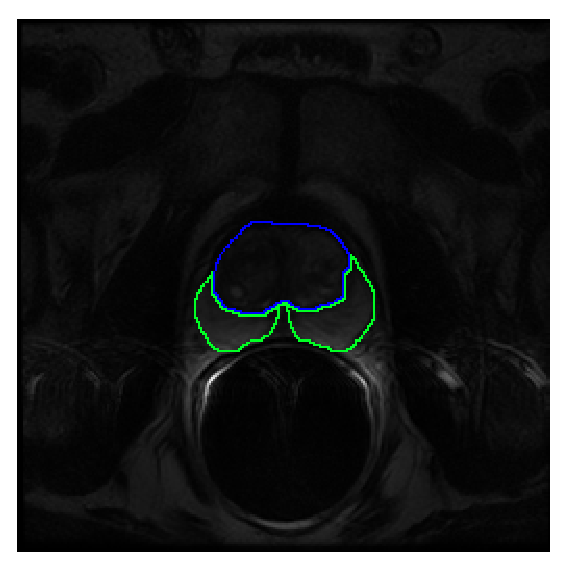
\includegraphics[width=0.3\linewidth]{02_background/figures/t2w/t2w_healthy.eps}} \hfill
	\subfigure[\ac{t2w}-ac{mri} slice of a prostate with a \ac{cap} highlighted in the \ac{pz} using a 3.0 Tesla \ac{mri} scanner.]{\label{subfig:t2wcancerpz}\includegraphics[width=0.3\linewidth]{02_background/figures/t2w/t2w_cancer_pz.eps}} \hfill
	\subfigure[\ac{t2w}-ac{mri} slice of a prostate with a \ac{cap} highlighted in the \ac{cg} using a 3.0 Tesla \ac{mri} scanner.]{\label{subfig:t2wcancercg}\includegraphics[width=0.3\linewidth]{02_background/figures/t2w/t2w_cancer_cg.eps}}
	\hspace*{\fill}
	\caption{Rendering of \ac{t2w}-\ac{mri} prostate image with both 1.5 and 3.0 Tesla \ac{mri} scanner.}
	\label{fig:t2w}
\end{figure*}

%T2W MRI
\item[$-$] \textbf{\textit{\ac{t2w} \ac{mri}:}} \ac{t2w} \ac{mri} was the first \ac{mri}-modality used to perform \ac{cap} diagnosis using \ac{mri} (\cite{Hricak1983}). Nowadays, radiologists make use of it for \ac{cap} detection, localization and staging purposes. This imaging technique is well suited to render zonal anatomy of the prostate (\cite{Barentsz2012}). 

This modality relies on a sequence based on setting a long \ac{tr}, reducing the T$_1$ effect in \ac{nmr} signal measured, and fixing the \ac{te} to sufficiently large values in order to enhance the T$_2$ effect of tissues. Thus, \ac{pz} and \ac{cg} tissues are well perceptible in these images. The former is characterized by an intermediate/high-\ac{si} while the latter is depicted by a low-\ac{si} (\cite{Hricak1987}). An example of a healthy prostate is shown in Fig. \ref{subfig:t2whealthy}.

In \ac{pz}, round or ill-defined low-SI masses are synonymous with \acp{cap} as shown in Fig. \ref{subfig:t2wcancerpz} (\cite{Hricak1983}). Detecting \ac{cap} in \ac{cg} is more challenging. In fact both normal \ac{cg} tissue and malignant tissue, have a low-\ac{si} in \ac{t2w} \ac{mri} reinforcing difficulties to distinguish between them. However, \acp{cap} in \ac{cg} appear often as homogeneous mass possessing ill-defined edges with lenticular or ``water-drop'' shapes as depicted in Fig. \ref{subfig:t2wcancercg} (\cite{Akin2006, Barentsz2012}). 

\ac{cap} aggressiveness was shown to be inversely correlated with \ac{si}. Indeed, \acp{cap} assessed with a \ac{gs} of 4-5 implied lower \ac{si} than the one with a \ac{gs} of 2-3 (\cite{Wang2008}).

In spite of the availability of these useful and encouraging features, the \ac{t2w} modality lacks reliability (\cite{Kirkham2006,Hoeks2011}). Sensitivity is affected by the difficulties in detecting cancers in \ac{cg} (\cite{Kirkham2006}) while specificity rate is highly affected by outliers (\cite{Barentsz2012}). In fact, various conditions emulate patterns of \ac{cap} such as \ac{bph}, post-biopsy haemorrhage, atrophy, scars and post-treatment (\cite{Hricak1987,Quint1991,Scheidler1999,Cruz2002,Barentsz2012}). These issues can be partly addressed using more innovative and advanced modalities.

%T2 Map
\item[$-$] \textbf{\textit{T$_2$ Map:}} As previously mentioned, \ac{t2w} \ac{mri} modality shows low sensitivity. Moreover, \ac{t2w} \ac{mri} images are a composite of multiple effects (\cite{Hegde2013}). However, T$_2$ values alone have been shown to be more discriminative (\cite{Liu2011}) and highly correlated with citrate concentration, a biological marker in \ac{cap} (\cite{Liney1996,Liney1997}). 

T$_2$ values are computed using the characteristics of transverse relaxation. Transverse relaxation is formalized as shown in \acs{eq} \ref{eq:tramag}.

\begin{equation}
	M_{x,y}(t) = M_{x,y}(0) \exp \left( - \frac{t}{\text{T}_2} \right) \ .
	\label{eq:tramag}
\end{equation}

\noindent where $M_{x,y}(0)$ is the initial value of $M_{x,y}(t)$ and T$_2$ is the relaxation time.

By rearranging \acs{eq} \ref{eq:tramag}, T$_2$ map is computed performing a linear fitting on the model in \acs{eq} \ref{eq:t2map} using several TE, $t=\{ \text{TE}_1,\text{TE}_2, \dotsc ,\text{TE}_m \}$.

\begin{equation}
	\ln \left[ \frac{M_{x,y}(t)}{M_{x,y}(0)} \right] = - \frac{t}{\text{T}_2} \ .
	\label{eq:t2map}
\end{equation}

\Ac{fse} sequence has been shown to be particularly well suited in order to build a T$_2$ map and obtain accurate T$_2$ values (\cite{Liney1996a}).

Such as \ac{t2w} \ac{mri}, T$_2$ values associated with \ac{cap} are significantly lower than those of healthy tissues (\cite{Liney1996,Gibbs2001}).

\begin{figure*}
\centering
	\hspace*{\fill}
	\subfigure[\ac{t1w}-\ac{mri} image where the cancer is delimited by the red contour. The green area was still not invaded by the \ac{cap}]{\label{subfig:t1w}\includegraphics[width=0.4\linewidth]{02_background/figures/dce/slice.eps}} \hfill
	\subfigure[Enhancement curve computed during the \ac{dce}-\ac{mri} analysis. The red curve is typical from \ac{cap} cancer while the green curve is characteristic of healthy tissue.]{\label{subfig:dce}\includegraphics[width=0.45\linewidth]{02_background/figures/dce/dce_cancer_healthy.eps}}
	\hspace*{\fill}
	\caption{Illustration of typical enhancement signal observed in \ac{dce}-\ac{mri} analysis collected with a 3.0 Tesla \ac{mri} scanner.}
	\label{fig:dceana}
\end{figure*}

%DCE MRI
\item[$-$] \textbf{\textit{\ac{dce} \ac{mri}:}} \ac{dce} \ac{mri} is an imaging technique which exploits the vascularity characteristic of tissues. Contrast media, usually gadolinium-based, is injected intravenously into the patient. The media extravasates from vessels to \ac{ees} and then released back into the vasculature before being eliminated by the kidneys (\cite{Gribbestad2005}). Furthermore, the diffusion speed of the contrast agent may vary due to several parameters: (i) the permeability of the micro-vessels, (ii) their surface area and (iii) the blood flow (\cite{Padhani2002}).

Healthy \ac{pz} is mainly made up of glandular tissue, around 70 \% (\cite{Choi2007}), which implies a reduced interstitial space restricting exchanges between vessels and \ac{ees} (\cite{Buckley2004,Niekerk2009}). Normal \ac{cg} has a more disorganised structure, composed of mainly fibrous tissue (\cite{Choi2007,Hoeks2011}) , which facilitates the arrival of the contrast agent in \ac{ees} (\cite{Niekerk2013}). To understand the difference between contrast media kinetic in malignant tumours and the two previous behaviours mentioned, one has to focus on the process known as angiogenesis (\cite{Carmeliet2000}). In order to ensure growth, malignant tumours produce and release angiogenic promoter substances (\cite{Carmeliet2000}). These molecules stimulate the creation of new vessels towards the tumour (\cite{Carmeliet2000}). However, the new vessel networks in tumours differ from those present in healthy tissue (\cite{Gribbestad2005}). They are more porous due to the fact that their capillary walls have a large number of ``openings'' (\cite{Gribbestad2005,Choi2007}). In contrast to healthy cases, this increased vascular permeability results in increased contrast agent exchanges between vessels and \ac{ees} (\cite{Verma2012}).

By making use of the previous aspects, \ac{dce} \ac{mri} is based on an acquisition of a set of \ac{t1w} \ac{mri} images over time. the Gadolinium-based contrast agent shortens T$_1$ relaxation time enhancing contrast in \ac{t1w} \ac{mri} images. The aim is to post-analyse the pharmacokinetic behaviour of the contrast media concentration in prostate tissues (\cite{Verma2012}). The image analysis is carried out in two dimensions: (i) in the spatial domain on a pixel-by-pixel basis and (ii) in the time domain corresponding to the consecutive images acquired with the \ac{mri}. Thus, for each spatial location, a signal linked to contrast media concentration is measured as shown in Fig. \ref{subfig:dce} (\cite{Tofts2010}). 

By taking the previous remarks regarding medical aspects and signal theory into account, \acp{cap} are characterized by a signal having an earlier and faster enhancement and an earlier wash-out (cf., the rate of the contrast agent flowing out of the tissue) (see Fig. \ref{subfig:dce}) (\cite{Verma2012}). Three different approaches exist to analyse these signals with the aim of tagging them as corresponding to either normal or malignant tissues. Qualitative analysis is based on assessment of the signal shape (\cite{Hoeks2011}). Quantitative approaches consist in inferring pharmocokinetic parameter values (\cite{Tofts2010}). Those parameters are part of mathematical-pharmacokinetic models which are directly based on physiological exchanges between vessels and \ac{ees}. Several pharmacokinetic models were proposed such as the Kety model (\cite{Kety1951}), the Tofts model (\cite{Tofts1997}) and mixed models (\cite{Larsson1996,StLawrence1998}). The last family of methods mixed both approaches and are grouped together under the heading of semi-quantitative methods. They rely on shape characterization using mathematical modelling to extract a set of parameters such as wash-in gradient, wash-out, integral under the curve, maximum signal intensity, time-to-peak enhancement and start of enhancement (see Fig. \ref{fig:dceana}) (\cite{Hoeks2011,Verma2012}). It was shown that semi-quantitative and quantitative methods improve localization of \ac{cap} when compared with qualitative methods (\cite{Rosenkrantz2013}). Section \ref{subsubsec:fddce} provides a full description of quantitative and semi-quantitative approaches.

\ac{dce} \ac{mri} combined with \ac{t2w} \ac{mri} has shown to enhance sensitivity compared to \ac{t2w} \ac{mri} alone (\cite{Jager1997,Kim2005,Schlemmer2004,Zelhof2009}). Despite this fact, \ac{dce} \ac{mri} possesses some drawbacks. Due to its ``dynamic'' nature, patient motions during the image acquisition lead to spatial misregistration of the image set (\cite{Verma2012}). Furthermore, it has been suggested that malignant tumours are difficult to distinguish from prostatitis located in \ac{pz} and \ac{bph} located in \ac{cg} (\cite{Hoeks2011,Verma2012}). These pairs of tissues tend to have similar appearances. Later studies have shown that \acp{cap} in \ac{cg} do not always manifest in homogeneous fashion. Indeed, tumours in this zone can present both hypo-vascularization and hyper-vascularization which illustrates the challenge of \ac{cap} detection in \ac{cg} (\cite{Niekerk2013}).

\begin{figure*}
\centering
	\hspace*{\fill}
	\subfigure[\ac{dw}-\ac{mri} image acquired with a 1.5 Tesla \ac{mri} scanner. Th cancer corresponds to the high \ac{si} region highlighted in red.]{\label{subfig:dwi}\includegraphics[width=0.25\linewidth]{02_background/figures/dwi/dwi_cancer.eps}} \hfill
	\subfigure[\ac{adc} map computer after acquisition of \ac{dw}-\ac{mri} iages with a 1.5 Tesla \ac{mri} scanner. Th cancer corresponds to the low \ac{si} region highlighted in red.]{\label{subfig:adc}\includegraphics[width=0.25\linewidth]{02_background/figures/dwi/adc_cancer.eps}}
	\hspace*{\fill}
	\caption{Illustration of of \ac{dw}-\ac{mri} and \ac{adc} map. The signal intensity corresponding to cancer are inversely correlated on these two types of imaging techniques.}
	\label{fig:dwi}
\end{figure*}

%DWI MRI
\item[$-$] \textbf{\textit{\ac{dw} \ac{mri}:}} As previously mentioned in the introduction (\acs{sec} \ref{sec:introduction}), \ac{dw} \ac{mri} is the most recent MRI imaging technique developed aiming at \ac{cap} detection and diagnosis (\cite{Scheidler1999}). This modality exploits the variations in motion of water molecules in different tissues (\cite{LeBihan1988,Koh2007}).

From a physiological point of view, the following facts can be claimed. On the one hand, \ac{pz}, as previously mentioned, is mainly glandular and tubular in structure allowing water molecules to move freely (\cite{Choi2007,Hoeks2011}). On the other hand, \ac{cg} is made up of muscular or fibrous tissue causing the motion of the water molecules to be more constrained and heterogeneous than in \ac{pz} (\cite{Hoeks2011}). Then, \ac{cap} growth leads to the destruction of normal glandular structure and is associated with an increase in cellular density (\cite{Hoeks2011,Koh2007,Somford2008}). Furthermore, these factors both have been shown to be inversely correlated with water diffusion (\cite{Koh2007,Somford2008}): higher cellular density implies a restricted water diffusion. Thus, water diffusion in \ac{cap} will be more restricted than both healthy \ac{pz} and \ac{cg} (\cite{Koh2007,Hoeks2011}).

From the \ac{nmr} principle side, \ac{dw} \ac{mri} sequence produces contrasted images due to variation of water molecules motion. The method is based on the fact that the signal in \ac{dw} \ac{mri} images is inversely correlated to the degree of random motion of water molecules (\cite{Huisman2003}). In fact, gradients are used in \ac{dw} \ac{mri} modality to encode spatial location of nuclei temporarily. Simplifying the problem in only one direction, a gradient is applied in that direction, dephasing the spins of water nuclei. Hence, the spin phases vary along the gradient direction depending of the gradient intensity at those locations. Then, a second gradient takes place in order to cancel the spin dephasing. Thus, the immobile water molecules will be subject to the same gradient intensity as the initial one while moving water molecules will be subject to a different gradient intensity. Thus, spins of moving water molecules will stay dephased whereas spins of immobile water molecules will come back in phase. As a consequence, a higher degree of random motion results into a more significant signal loss whereas a lower degree of random motion is synonymous with lower signal loss (\cite{Huisman2003}). Under these conditions, the MRI signal measured is formalized as in \acs{eq} \ref{eq:t2dif}.

\begin{equation}
	M_{x,y}\left(t,b\right) = M_{x,y}(0) \exp \left( - \frac{t}{\text{T}_2} \right) S_{\text{ADC}}(b) \ , 
	\label{eq:t2dif}
\end{equation}

\begin{equation}
	S_{\text{ADC}}(b) = \exp \left( -b \times \text{ADC} \right) \ . 
	\label{eq:dif}
\end{equation}

\noindent where $S_{\text{ADC}}$ refers to signal drop due to diffusion effect, $\text{ADC}$ is the \acl{adc} and $b$ is the attenuation coefficient depending only on gradient pulses parameters: (i) gradient intensity and (ii) gradient duration (\cite{LeBihan1986}).

By using this formulation, image acquisition with a parameter $b=0$ s.mm$^{-2}$ corresponds to a \ac{t2w} \ac{mri} acquisition. Then, increasing the attenuation coefficient $b$ (cf., increase gradient intensity and duration) enhances the contrast in \ac{dw} \ac{mri} images.

To summarize, in \ac{dw} \ac{mri} images, \acp{cap} are characterized by high-\ac{si} compared to normal tissues in \ac{pz} and \ac{cg} as shown in Fig. \ref{subfig:dwi} (\cite{Barentsz2012}). However, some tissues in \ac{cg} can look similar to \ac{cap} with higher \ac{si} (\cite{Barentsz2012}).

Diagnosis using \ac{dw} \ac{mri} combined with \ac{t2w} \ac{mri} has shown significant improvement compared with \ac{t2w} \ac{mri} alone and provides highly contrasted images (\cite{Shimofusa2005,Padhani2011,Choi2007}). As drawbacks, this modality suffers from poor spatial resolution and specificity due to false positive detection (\cite{Choi2007}).

With a view to eliminate these drawbacks, radiologists are extracting quantitative maps from \ac{dw} \ac{mri}. This imaging technique is presented next.

%ADC map
\item[$-$] \textbf{\textit{\ac{adc} Map:}} The \ac{nmr} signal measured for \ac{dw} \ac{mri} images is not only affected by diffusion as shown in \acs{eq} \ref{eq:t2dif}. However, the signal drop (\acs{eq} \ref{eq:dif}) is formulated such that the only variable is the acquisition parameter $b$ (\cite{LeBihan1986}). The \ac{adc} is considered as a ``pure'' diffusion coefficient and can be extracted to build a quantitative map.

From \acs{eq} \ref{eq:t2dif}, it is clear that performing multiple acquisitions only varying $b$ will not have any effect on the term  $M_{x,y}(0) \exp \left( - \frac{t}{\text{T}_2} \right)$. Thus, \acs{eq} \ref{eq:t2dif} can be rewritten as:

\begin{equation}
	S(b) = S_0 \exp \left( -b \times \text{ADC} \right) \ .
	\label{eq:t2adcrew}
\end{equation}

To compute the \ac{adc} map, a minimum of two acquisitions is necessary: (i) for $b_0=0$ s.mm$^{-2}$ where the measured signal is equal to $S_0$, and (ii) $b_1>0$ s.mm$^{-2}$ (typically $1000$ s.mm$^{-2}$). Then, the \ac{adc} map can be computed as:

\begin{equation}
	\text{ADC} = - \frac{\ln \left( \cfrac{S(b_1)}{S_0} \right) }{b_1} \ .
	\label{eq:adcres1}
\end{equation}

More accurate computation of the \ac{adc} map can be obtained by performing several acquisitions with different values for the parameter $b$ and performing a semi-logarithmic linear fitting using the model presented in \acs{eq} \ref{eq:t2adcrew}.

Regarding the appearance of the \ac{adc} maps, it was previously stated that by increasing the value of $b$, the signal of \ac{cap} tissue increases significantly. From \acs{eq} \ref{eq:adcres1}, it can be shown that tissue appearance in the ADC map will be the reverse of \ac{dw} \ac{mri} images. Then, \ac{cap} tissue is associated with low-\ac{si} whereas healthy tissue appears brighter as depicted in Fig. \ref{subfig:adc} (\cite{Barentsz2012}).

Similar to the gain achieved by \ac{dw} \ac{mri}, diagnosis using \ac{adc} map combined with \ac{t2w} \ac{mri} significantly outperforms \ac{t2w} \ac{mri} alone (\cite{Doo2012,Choi2007}). Moreover, it has been shown that \ac{adc} is correlated with \ac{gs} (\cite{Hambrock2011, Itou2011, Peng2013}).

However, some tissues of the \ac{cg} zone mimic \ac{cap} with low-\ac{si} (\cite{Kirkham2006}). Image distortion can arise due to haemorrhage (\cite{Choi2007}). It has also been noted that high variation of the \ac{adc} occurs between patients making difficult to define a static threshold to distinguish \ac{cap} from non-malignant tumours (\cite{Choi2007}). 

\begin{figure*}
	\centering
	\hspace*{\fill}
	\subfigure[Illustration of an \ac{mrsi} spectrum of an healthy voxel acquired with a 3.0 Tesla \ac{mri}.]{\label{subfig:mrsihea}\includegraphics[width=0.45\linewidth]{02_background/figures/mrsi/mrsi_healthy.eps}} \hfill
	\subfigure[Illustration of an \ac{mrsi} spectrum of a cancerous voxel acquired with a 3.0 Tesla \ac{mri}.]{\label{subfig:mrsican}\includegraphics[width=0.45\linewidth]{02_background/figures/mrsi/mrsi_cancer.eps}}
	\hspace*{\fill}
	\caption{Illustration of an \ac{mrsi} spectrum both healthy and cancerous voxel with a 3.0 Tesla \ac{mri}. The highlighted areas corresponds to the integrated area used for quantification. Acronyms: Choline (Cho), Spermine (Spe), Creatine (Cr) and Citrate (Cit).}
	\label{fig:mrsi}
\end{figure*}

%MRSI
\item[$-$] \textbf{\textit{\ac{mrsi}:}} \ac{cap} induces metabolic changes in the prostate compared with healthy tissue. Thus, \ac{cap} detection can be carried out by tracking changes of metabolite concentration in prostate tissue. \ac{mrsi} is an \ac{nmr}-based technique which generates spectra of relative metabolite concentration in \iac{roi}.

In order to track changes of metabolite concentration, it is important to know which metabolites are associated with \ac{cap}. To address this question, clinical studies identified three biological markers: (i) citrate, (ii) choline and (iii) polyamines composed mainly of spermine, and in less abundance of spermidine and putrescine (\cite{Awwad2012,Costello2006,Giskeodegard2013}). 

Citrate is involved in the production and secretion of the prostatic fluid, and the glandular prostate cells are associated with a high production of citrate enabled by zinc accumulation by these same cells (\cite{Costello2006}). However, the metabolism allowing the accumulation of citrate requires a large amount of energy (\cite{Costello2006}). In contrast, malignant cells do not have high zinc levels leading to lower citrate levels due to citrate oxydation (\cite{Costello2006}). Furthermore, this change results in a more energy-efficient metabolism enabling malignant cells to grow and spread (\cite{Costello2006}).

An increased concentration of choline is related to \ac{cap} (\cite{Awwad2012}). Malignant cell development requires epigenetic mechanisms resulting in metabolic changes and relies on two mechanisms: DNA methylation and phospholid metabolism which both result in choline uptake, explaining its increased level in \ac{cap} tissue (\cite{Awwad2012}).

Spermine is also considered as a biological marker in \ac{cap} (\cite{Graaf2000,Giskeodegard2013}). In \ac{cap}, reduction of the ductal volume due to shifts in polyamine homeostasis might lead to a reduced spermine concentration (\cite{Graaf2000}).

To determine the concentration of these biological markers, one has to focus on the \ac{mrsi} modality. In theory, in presence of a homogeneous magnetic field, identical nuclei precesses at the same operating frequency known as the Lamor frequency (\cite{Haacke1999}). However, \ac{mrsi} is based on the fact that identical nuclei will slightly precess at different frequencies depending on the chemical environment in which they are immersed (\cite{Haacke1999}). A phenomenon known as the \ac{cse} (\cite{Parfait2010}). Given this property, metabolites can be identified and their concentrations can be determined. In this regard, the Fourier transform is used to obtain the frequency spectrum of the \ac{nmr} signal (\cite{Haacke1999,Parfait2010}). In this spectrum, each peak is associated with a particular metabolite and the area under each peak corresponds to the relative concentration of this metabolite (see Fig. \ref{fig:mrsi}) (\cite{Parfait2010}).

Hence, frequencies of interest in regard to \ac{cap} detection and diagnosis should correspond to the earlier mentioned metabolites. Choline and spermine are represented by a single peak at respectively 3.21 ppm and 3.11 ppm (\cite{Verma2010}). Due to the coupling effect, citrate is represented by three or four peaks depending on the magnetic field strength. Citrate ranges from 2.47 ppm to 2.81 ppm with a central frequency at 2.64 ppm (\cite{Verma2010}). Then, relative concentrations of these metabolites are obtained by computing the area under the curve of the spectrum between the lower and upper frequency limits of each peak.

Two different quantitative approaches are used to decide either or not the spectra of \iac{roi} is associated with \ac{cap} classified either as relative quantification or absolute quantification (\cite{Lemaitre2011}). In relative quantification, the ratio of choline-polyamines-creatine to citrate is computed. Integral of the signal is computed from choline (cf., 3.21 ppm) to creatine (cf., 3.02 ppm) because the peaks in this region can be merged at clinical magnetic field strengths (see Fig. \ref{fig:mrsi}) (\cite{Hoeks2011,Graaf2000}). Considering the previous assumption that choline concentration rises and citrate concentration decreases in the presence of \ac{cap}, the ratio computed should be higher in malignant tissue than in healthy tissue. 

In contrast with relative quantification, absolute quantification measures molar concentrations by normalizing relative concentrations using water as reference (\cite{Lemaitre2011}). In this case, ``true'' concentrations are directly used to differentiate malignant from healthy tissue. However, this method is not commonly used as it requires an additional step of acquiring water signals, inducing time and cost acquisition constraints.

\ac{mrsi} allows examination with high specificity and sensitivity compared to others \ac{mri} modalities (\cite{Choi2007}). Furthermore, it has been shown that combining \ac{mrsi} with \ac{mri} improves detection and diagnosis performance (\cite{Scheidler1999a,Kaji1998}). Citrate and spermine concentration are inversely correlated with the \ac{gs} allowing us to distinguish low from high grade \acp{cap} (\cite{Giskeodegard2013}). However, choline concentration does not provide the same properties (\cite{Giskeodegard2013}).

Unfortunately, \ac{mrsi} also presents several drawbacks. First, \ac{mrsi} acquisition is time consuming which makes this modality not normally used in clinical daily practise (\cite{Barentsz2012}). In addition, \ac{mrsi} suffers from low spatial resolution due to the fact that \ac{snr} is linked to the voxel size. However, this issue is addressed by developing new scanners with higher magnetic field strengths such as 7.5 T (\cite{Giskeodegard2013}). Finally, a high variability of the relative concentrations between patients was observed (\cite{Choi2007}). The same observation was made depending on the zones studied (cf., \ac{pz}, \ac{cg}, base, mid-gland, apex) (\cite{Walker2010,Lemaitre2011}). Due to this variability, it is difficult to use a fixed thresholds in order to differentiate \ac{cap} from healthy tissue.

\end{enumerate}

\subsubsection{Computer-aided systems for \ac{cap}: \ac{cade} - \ac{cadx}} \label{subsubsec:CAD}

As previously mentioned in the introduction (see \acs{sec} \ref{sec:introduction}), \acp{cad} are developed to advise and backup radiologists in their tasks of \ac{cap} detection and diagnosis; \acp{cad} are not aimed to provide fully automatic decisions (\cite{Giger2008}). \acp{cad} can be divided into two different sub-groups either as \ac{cade}, with the purpose to highlight probable lesions in \ac{mri} images, or \ac{cadx}, which focuses more in details differentiate malignant from non-malignant tumours (\cite{Giger2008}). Moreover, an intuitive approach, motivated by developing a framework combining detection-diagnosis, is to mix both \ac{cade} and \ac{cadx} by using the output of the former mentioned as input of the latter named. Although the outcomes of these two systems should differ, the framework of both \ac{cad} systems is similar. The \ac{cad} work-flow is presented in \acs{fig} \ref{fig:wkfcad}.

\ac{mri} modalities mentioned in \acs{sec} \ref{subsubsec:mrimrsi} are used as inputs of \ac{cad} for \ac{cap}. It can be noted that \ac{adc} map is not considered as an input since that it is a feature derived from the \ac{dw} \ac{mri} images. The images acquired from the different modalities show a large variability between patients: the prostate organ can be located at different positions in images (e.g., patient motion, variation of acquisition plan), the \ac{si} can be corrupted with noise or artefacts during the acquisition process (eg., magnetic field inhomogeneity, use of endorectal coil). To address these issues, the first stage of \ac{cad} is to pre-process multiparametric \ac{mri} images to reduce noise, remove artefacts and standardize the \ac{si}. Then, it is important to mention that later processes should only investigate the prostate organ. Thus, it is necessary to segment the prostate in each \ac{mri}-modality to define it as \iac{roi}. However, data suffers of misalignment due to patient motions or different acquisition plan. Therefore, a registration step is performed so that all the previously segmented \ac{mri} images will be in the same reference frame.

Some studies does not fully apply the methodology depicted in \acs{fig} \ref{fig:wkfcad}. Details about those can be found in \acs{tab} \ref{tab:sumpap}. Some studies preferred to work directly with raw data in order to demonstrate the robustness of their approaches to noise or artefacts. In some cases, prostate segmentation is performed manually as well as registration. It is also sometimes assumed that no patient motions occur during the acquisition procedure, lowering the need of registering the multiparametric \ac{mri} images.

Once the data are regularized, it becomes possible to extract features and classify the data to obtain the probabilistic maps. We refereed this stage to image classification where \ac{cade} and \ac{cadx} are the main components. 

In \iac{cade} framework, possible lesions will be segmented automatically to further classify them as malignant or non-malignant. We also included in \ac{cade} studies which considered all voxels as \acp{roi} but in which malignant lesions will be highlighted after the classification stage. However, manual lesions segmentation are not considered as part of \iac{cade}. Therefore, \acp{roi} manually selected or detected through \iac{cade} system are used as inputs of \iac{cadx}.

\Ac{cadx} is composed of the processes allowing to distinguish malignant from non-malignant tumours. We divided \ac{cadx} into three different stages. First, salient features are extracted from \ac{mri} images to characterize the scene. Of course, more discriminative features will be associated with robust and accurate likelihood cancer map. Most frequently, the number of feature extracted can be large resulting in redundant or not enough discriminative features which will negatively affect the performances of the further classification. Therefore, a step consisting at selecting the best features or/and reducing the number of dimensionality is commonly used. Then, this modified feature vector is finally classified using different pattern recognition approaches.

As pointed out in the introduction (see \acs{sec} \ref{sec:introduction}), performances of \ac{cap} detection and diagnosis is affected by observer interpretation and limitations (\cite{Giger2008,Hambrock2013}). \ac{cad} offers a possible solution in order to reduce this variability. Lately, effect of \ac{cad} on the observer performance has been studied (\cite{Hambrock2013}). Results shown that \acp{cad} benefit to less-experienced radiologist to perform similarly as experienced radiologist in their tasks (\cite{Hambrock2013}). 

\subsection{Literature classification}

\newgeometry{left=1cm,right=1cm,bottom=0.5cm,top=0.3cm}

\begin{table*}
\centering
\caption{Overview of the different studies reviewed with their main characteristics. Acronyms: number (\#) - image regularization (Img. Reg.).}
\scriptsize
%\begin{adjustwidth}{-1.5cm}{}
\begin{threeparttable}
\renewcommand{\arraystretch}{1.5}	
	\rowcolors{3}{black!5}{white}	
	\begin{tabular}{|>{\centering\arraybackslash}m{0.7cm}|>{\centering\arraybackslash}m{3.3cm}|>{\centering\arraybackslash}m{1cm}|>{\centering\arraybackslash}m{0.8cm}>{\centering\arraybackslash}m{0.8cm}>{\centering\arraybackslash}m{1cm}>{\centering\arraybackslash}m{1cm}|>{\centering\arraybackslash}m{0.7cm}>{\centering\arraybackslash}m{0.7cm}|>{\centering\arraybackslash}m{0.7cm}>{\centering\arraybackslash}m{0.7cm}|>{\centering\arraybackslash}m{0.7cm}>{\centering\arraybackslash}m{0.7cm}>{\centering\arraybackslash}m{0.7cm}|}\hline
	\hiderowcolors
	\multirow{2}{*}{Index} & \multirow{2}{*}{Study} & \# & \multicolumn{4}{c|}{\ac{mri}-modality} & \multicolumn{2}{c|}{Strength of field} & \multicolumn{2}{c|}{Studied zones} & \multicolumn{3}{c|}{\ac{cad} stages} \\ \cline{4-14}
	 & & patients & \ac{t2w} \ac{mri} & \ac{dce} \ac{mri} & \ac{dw} \ac{mri} & \ac{mrsi} & 1.5 T & 3.0 T & \ac{pz} & \ac{cg} & Img. Reg. & \ac{cade} & \ac{cadx} \\ \hline \hline
	 \showrowcolors 
	 	 $[1]$&\cite{Ampeliotis2007} & 25 & \cmark & \cmark & \xmark & \xmark & \cmark & \xmark & \cmark & \xmark & \mmark & \xmark & \cmark \\
	 	 $[2]$&\cite{Ampeliotis2008} & 25 & \cmark & \cmark & \xmark & \xmark & \cmark & \xmark & \cmark & \xmark & \mmark & \xmark & \cmark \\
	 	 $[3]$&\cite{Antic2013} & 53 & \cmark & \xmark & \cmark & \xmark & \cmark & \xmark & \cmark & \cmark & \xmark  & \xmark & \cmark \\
	 	 $[4]$&\cite{Artan2009} & 10 & \cmark & \cmark & \cmark & \xmark & \cmark & \xmark & \cmark & \xmark  & \xmark & \cmark & \cmark \\
	 	 $[5]$&\cite{Artan2010} & 21 & \cmark & \cmark & \cmark & \xmark & \cmark & \xmark & \cmark & \xmark & \mmark & \cmark & \cmark \\
	 	 $[6]$&\cite{Chan2003} & 15 & \cmark & \xmark & \cmark & \xmark & \cmark & \xmark & \cmark & \xmark & \xmark & \xmark & \cmark \\
	 	 $[7]$&\cite{Giannini2013} & 10 & \cmark & \cmark & \cmark & \xmark & \cmark & \xmark & \cmark & \xmark & \cmark & \cmark & \cmark \\
	 	 $[8]$&\cite{Kelm2007} & 24 & \xmark & \xmark & \xmark & \cmark & \cmark & \xmark & \cmark & \cmark & \mmark & \cmark & \cmark \\
	 	 $[9]$&\cite{Langer2009} & 25 & \cmark & \cmark & \cmark & \xmark & \cmark & \xmark & \cmark & \xmark & \mmark & \xmark & \cmark \\
	 	 $[10]$&\cite{Litjens2011} & 188 & \cmark & \cmark & \cmark & \xmark & \xmark & \cmark & \cmark & \xmark & \mmark & \cmark & \cmark \\
	 	 $[11]$&\cite{Litjens2012} & 288 & \cmark & \cmark & \cmark & \xmark & \xmark & \cmark & \cmark & \cmark & \mmark & \cmark & \cmark \\
	 	 $[12]$&\cite{Liu2009} & 11 & \cmark & \cmark & \cmark & \xmark & \cmark & \xmark & \cmark & \xmark & \mmark & \cmark & \cmark \\
	 	 $[13]$&\cite{Liu2013} & 54 & \cmark & \cmark & \cmark & \xmark & \xmark & \cmark & \cmark & \cmark & \mmark & \xmark & \cmark \\
	 	 $[14]$&\cite{Lopes2011} & 27 & \cmark & \xmark & \xmark & \xmark & \cmark & \xmark & \cmark & \xmark & \mmark & \cmark & \cmark \\
	 	 $[15]$&\cite{Lv2009} & 55 & \cmark & \xmark & \xmark & \xmark & \cmark & \xmark & \cmark & \xmark & \mmark & \xmark & \cmark \\
	 	 $[16]$&\cite{Matulewicz2013} & 18 & \xmark & \xmark & \xmark & \cmark & \xmark & \cmark & \cmark & \cmark & \xmark & \cmark & \cmark \\ 
	 	 $[17]$&\cite{Mazzetti2011} & 10 & \xmark & \cmark & \xmark & \xmark & \cmark & \xmark & \cmark & \xmark & \mmark & \cmark & \cmark \\
	 	 $[18]$&\cite{Niaf2011} & 23 & \cmark & \cmark & \cmark & \xmark & \cmark & \xmark & \cmark & \xmark & \mmark & \xmark & \cmark \\
	 	 $[19]$&\cite{Niaf2012} & 30 & \cmark & \cmark & \cmark & \xmark & \cmark & \xmark & \cmark & \xmark & \mmark & \xmark & \cmark \\
	 	 $[20]$&\cite{Ozer2009} & 20 & \cmark & \cmark & \cmark & \xmark & \cmark & \xmark & \cmark & \xmark & \mmark & \cmark & \cmark \\
	 	 $[21]$&\cite{Ozer2010} & 20 & \cmark & \cmark & \cmark & \xmark & \cmark & \xmark & \cmark & \xmark & \mmark & \cmark & \cmark \\
	 	 $[22]$&\cite{Parfait2012} & 22 & \xmark & \xmark & \xmark & \cmark & \xmark & \cmark & \cmark & \cmark & \mmark & \cmark & \cmark \\
	 	 $[23]$&\cite{Peng2013} & 48 & \cmark & \cmark & \cmark & \xmark & \xmark & \cmark & \cmark & \cmark & \xmark & \xmark & \cmark \\
	 	 $[24]$&\cite{Puech2009} & 100 & \xmark & \cmark & \xmark & \xmark & \cmark & \xmark & \cmark & \cmark & \xmark & \xmark & \cmark \\
	 	 $[25]$&\cite{Sung2011} & 42 & \xmark & \cmark & \xmark & \xmark & \xmark & \cmark & \cmark & \cmark & \xmark & \cmark & \cmark \\
	 	 $[26]$&\cite{Tiwari2007} & 14 & \xmark & \xmark & \xmark & \cmark & \cmark & \xmark & \cmark & \cmark & \mmark & \cmark & \cmark \\
	 	 $[27]$&\cite{Tiwari2008} & 18 & \xmark & \xmark & \xmark & \cmark & \cmark & \xmark & \cmark & \cmark & \mmark & \cmark & \cmark \\
	 	 $[28]$&\cite{Tiwari2009} & 18 & \xmark & \xmark & \xmark & \cmark & \cmark & \xmark & \cmark & \cmark & \mmark & \cmark & \cmark \\
	 	 $[29]$&\cite{Tiwari2009a} & 15 & \cmark & \xmark & \xmark & \cmark & \cmark & \xmark & \cmark & \cmark & \mmark & \cmark & \cmark \\
	 	 $[30]$&\cite{Tiwari2010} & 19 & \cmark & \xmark & \xmark & \cmark & \cmark & \xmark & \cmark & \cmark & \mmark & \cmark & \cmark \\
	 	 $[31]$&\cite{Tiwari2012} & 36 & \cmark & \xmark & \xmark & \cmark & \cmark & \xmark & \cmark & \cmark & \xmark & \cmark & \cmark \\
	 	 $[32]$&\cite{Tiwari2013} & 29 & \cmark & \xmark & \xmark & \cmark & \cmark & \xmark & \cmark & \cmark & \mmark & \cmark & \cmark \\
	 	 $[33]$&\cite{Viswanath2008} & 16 & \cmark & \xmark & \xmark & \cmark & \cmark & \xmark & \cmark & \cmark & \xmark & \cmark & \cmark \\
	 	 $[34]$&\cite{Viswanath2008a} & 6 & \cmark & \cmark & \xmark & \xmark & \xmark & \cmark & \cmark & \cmark & \mmark & \cmark & \cmark \\
	 	 $[35]$&\cite{Viswanath2009} & 6 & \cmark & \cmark & \xmark & \xmark & \xmark & \cmark & \cmark & \cmark & \cmark & \cmark & \cmark \\
	 	 $[36]$&\cite{Viswanath2011} & 12 & \cmark & \cmark & \cmark & \xmark & \xmark & \cmark & \cmark & \cmark & \mmark & \cmark & \cmark \\
	 	 $[37]$&\cite{Viswanath2012} & 22 & \cmark & \xmark & \xmark & \xmark & \xmark & \cmark & \cmark & \cmark & \cmark & \cmark & \cmark \\
	 	 $[38]$&\cite{Vos2008} & 29 & \cmark & \cmark & \xmark & \xmark & \cmark & \xmark & \cmark & \xmark & \mmark & \xmark & \cmark \\
	 	 $[39]$&\cite{Vos2008a} & 29 & \xmark & \cmark & \xmark & \xmark & \cmark & \xmark & \cmark & \xmark & \mmark & \xmark & \cmark \\
	 	 $[40]$&\cite{Vos2010} & 29 & \cmark & \cmark & \xmark & \xmark & \cmark & \xmark & \cmark & \xmark & \mmark & \xmark & \cmark \\
	 	 $[41]$&\cite{Vos2012} & NA & \cmark & \cmark & \cmark & \xmark & \xmark & \cmark & \cmark & \xmark & \mmark & \cmark & \cmark \\
	 	 \hline
	\end{tabular}
	\begin{tablenotes}
      \tiny
      \item Notes:
      \item {\xmark}: not used or not implemented.
      \item {\mmark}: partially implemented.
      \item {\cmark}: used or implemented.
    \end{tablenotes}
\end{threeparttable}
%\end{adjustwidth}
\label{tab:sumpap}
\end{table*}

\restoregeometry

The review will be organized using the methodology presented in \acs{fig} \ref{fig:wkfcad}. Methods embedded in the image regularization framework will be presented before to focus on the image classification framework. This latter mentioned will be divided into \ac{cade} and \ac{cadx}. \Acl{tab} \ref{tab:sumpap} summarizes the different \ac{cad} studies reviewed in this paper. Characteristics related to \ac{mri} acquisition as well as \ac{cad} strategies are reported. Only methods used in \ac{cad} system will be discussed.

\section{Image regularization framework} \label{sec:imaprocfra}

This section provides a review of the methods used in \acp{cad} in order to regularize input images. We start with pre-processing methods presented in Sect. \ref{subsec:preprocessing}, focusing mainly on the reduction of noise level and artefacts as well as standardization of \ac{si}. Sections \ref{subsec:segmentation} and \ref{subsec:registration} will be dedicated to segmentation methods, so that later methods only operate on the segmented prostate, and registration to align segmented images from different \ac{mri}-modalities in the same reference frame.

\def\rmm#1{{\bf \sc Robert: }{\marrow\sf #1}}


\subsection{Pre-processing} \label{subsec:preprocessing}

\begin{table}
	\caption{Overview of the pre-processing methods used in \ac{cad} systems.}
	\small
	%\renewcommand{\arraystretch}{1.5}
	\begin{tabular}{p{.65\linewidth} p{.25\linewidth}}
		\hline \\ [-1.5ex]
		\textbf{Pre-processing operations} & \textbf{References} \\ \\ [-1.5ex]
		\hline \\ [-1.5ex]
		\textit{\ac{mri} pre-processing:} & \\ \\ [-1.5ex]
		\quad Noise filtering: &  \\
		\quad \quad Median filtering & $[$22-23$]$  \\
		\quad \quad Wavelet-based filtering & $[$1-2,15$]$ \\ \\ [-1.5ex]
		\quad Bias correction: & \\
		\quad \quad Parametric methods & $[$16,36$]$ \\
		\quad \quad Non-parametric methods & $[$37$]$ \\ \\ [-1.5ex]
		\quad Standardization: & \\
		\quad \quad Statistical-based normalization: & $[$3-4,16,21-22,36,38$]$ \\
		\quad \quad Organ \ac{si}-based normalization & $[$19-20$]$ \\ \\ [-1.5ex]
		\textit{\ac{mrsi} pre-processing:} & \\ \\ [-1.5ex]
		\quad Phase correction & $[$23$]$ \\
		\quad Water and lipid residuals filtering & $[$8$]$ \\
		\quad Baseline correction & $[$23,32$]$ \\
		\quad Frequency alignment & $[$32$]$ \\
		\quad Normalization & $[$23$]$ \\ \\ [-1.5ex]
		\hline
	\end{tabular}
\end{table}

\subsubsection{\ac{mri} images pre-processing}

Three different groups of pre-processing methods are commonly applied to images as initial stage in \ac{cad}.

\setenumerate{listparindent=\parindent,itemsep=10px}
\setlist{noitemsep}
\begin{enumerate}[leftmargin=*]

%\begin{figure}
%\centering
%	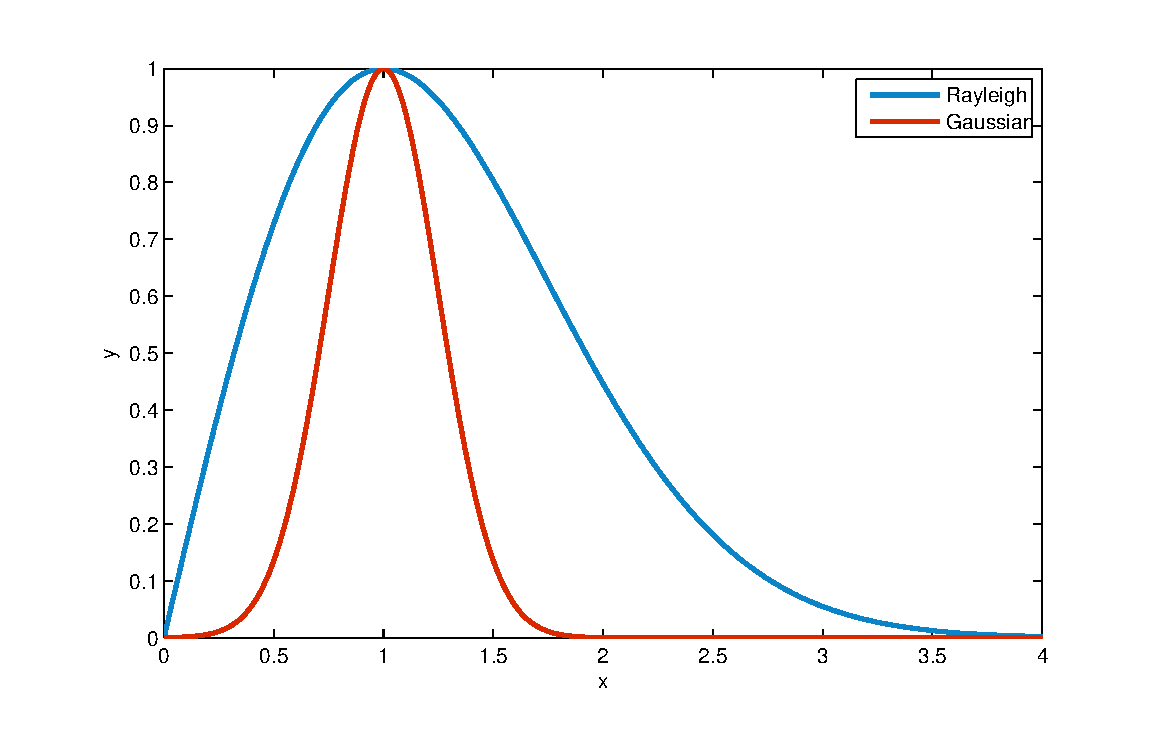
\includegraphics[width=0.9\linewidth]{03_image_processing/03_preprocessing/figures/noise/noisedistr.eps}
%	\caption{Illustration of a Gaussian distribution ($\mu = 1, \sigma=0.25$) and a Rayleigh distribution ( $\sigma = 2$). It can be seen that the Rayleigh distribution is suffering of a bias term when compared with the Gaussian distribution.}
%	\label{fig:noisedistr}
%\end{figure}

%Noise filtering
\item[$-$] \textbf{\textit{Noise filtering:}} The \ac{nmr} signal measured and recorded in the k-space during an \ac{mri} acquisition is affected by noise. This noise obeys a complex Gaussian white noise mainly due to thermal noises in the patient area (\cite{Nowak1999}). Furthermore, \ac{mri} images visualized by radiologists are in fact the magnitude images resulting from the complex Fourier transform of the k-space data. The complex Fourier transform, being a linear and orthogonal transform, does not affect the Gaussian noise characteristics (\cite{Nowak1999}). However, the function involved in the magnitude computation is a non-linear transform (i.e., the square root of the sum of squares of real and the imaginary parts), implying that the noise distribution is no longer Gaussian; it indeed follows a Rician distribution making the denoising task harder. Briefly, a Rician distribution can be characterized as follows: in low-\ac{si} region (low \ac{snr}), it can be approximated with a Rayleigh distribution while in high-\ac{si} region (high \ac{snr}), it is similar to a Gaussian distribution (\cite{Manjon2008}). Reviews of all denoising methods can be found in the work of \cite{Buades2005} and \cite{Mohan2014}.

Median filtering is the simplest approach used to address the denoising issue in \ac{mri} images (\cite{Ozer2009,Ozer2010}). %In both studies, Ozer et al. used a square kernel of size $5 \times 5$ pixels with the image resolutions ranging from $320 \times 256$ (cf., \ac{t2w} \ac{mri}) to $256 \times 128$ (cf., T$_2$ map, \ac{dce} and \ac{dw} \ac{mri}) and \iac{fov} ranging from 14 cm (cf, \ac{t2w} and \ac{dw} \ac{mri}) to 20 cm (cf, T$_2$ map and \ac{dce} \ac{mri}). 
However, from a theoretical point of view, this simple filtering method is not well formalized to address the noise distribution in \ac{mri} images.

More complex approaches were proposed to overcome this problem. A common method used to denoise \ac{mri} images is based on wavelet-based filtering. % This filtering exploits the sparsity property of the wavelet decomposition. The projection of a noisy signal from the spatial-domain to the wavelet-domain implies that only few wavelet coefficients contribute to the ``signal-free noise'' while all wavelet coefficients contribute to the noise (\cite{Donoho1994}). Therefore, denoising is performed by thresholding/attenuating the insignificant wavelet coefficients to enforce the sparsity in the wavelet-domain. 
Investigations focus on the strategies to perform the most adequate coefficient shrinkage method (e.g., using thresholding, singularity property or Bayesian framework) (\cite{Pizurica2002}).

\cite{Ampeliotis2007,Ampeliotis2008} performed wavelet shrinkage to denoise magnitude \ac{mri} images (cf., \ac{t2w}-\ac{mri} and \ac{dce}-\ac{mri}) using thresholding techniques (\cite{Mallat2008}). However, since the wavelet transform is an orthogonal transform, the Rician distribution of the noise is preserved in the wavelet-domain. Hence, for low \ac{snr}, the wavelet and scaling coefficients still suffer from a bias due to this specific noise distribution (\cite{Nowak1999}). 

\cite{Lopes2011} used the filtering technique proposed by \cite{Pizurica2003} to denoise \ac{t2w}-\ac{mri} which was based on joint detection and estimation theory (\cite{Middleton1968}).% The wavelet coefficients ``free-of-noise'' are estimated from the noisy wavelet coefficients using a \ac{map} estimate. Furthermore, the estimator designed takes spatial context into account by including both local and global information in the prior probabilities. The different probabilities needed by the \ac{map} are empirically estimated by using mask images representing the locations of the significant wavelet coefficients. These mask images are computed by thresholding the detail images obtained from the wavelet decomposition. To remove the bias from the wavelet and scaling coefficients, the squared magnitude \ac{mri} image used instead of the magnitude \ac{mri} image as proposed by \cite{Nowak1999}. This involves changing the Rician distribution to a scaled non-central Chi-square distribution. It implies that the wavelet coefficients are also unbiased estimators and the scaling coefficients are unbiased estimators but up to a constant $C$ as defined in Eq. \eqref{eq:nowakC} which needs to be subtracted from each scaling coefficient,

%\begin{equation}
%	C=2^{(J+1)}\hat{\sigma}^2 \ ,
%	\label{eq:nowakC}
%\end{equation}
%
%\noindent where $J$ is the number of levels of the wavelet decomposition and $\hat{\sigma}$ is an estimate of the noise standard deviation.
%
%\begin{figure}
%\centering
%	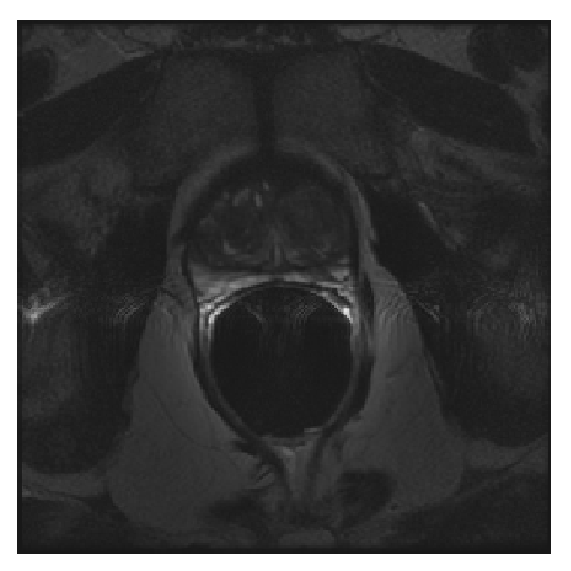
\includegraphics[width=0.5\linewidth]{03_image_processing/03_preprocessing/figures/bias/t2w_bias_antenna.eps}
%	\caption{Example of artefacts with high \ac{si} due to perturbation from the endorectal coil which create inhomogeneity.}
%	\label{fig:bias}
%\end{figure}

% Artefacts filtering
\item[$-$] \textbf{\textit{Bias correction:}} Besides being corrupted by noise, \ac{mri} images are also affected by the inhomogeneity of the \ac{mri} field commonly referred to as bias field (\cite{Styner2000}). This bias field results in a smooth variation of the \ac{si} through the image. When an endorectal coil is used, an artefact resulting of an hyper-intense signal can be observed around the coil on the images. As a consequence, the \ac{si} of identical tissues varies depending on their spatial location in the image making further processes such as segmentation or registration harder (\cite{Jungke1987,Vovk2007}). A review of bias correction methods can be found in \cite{Vovk2007}.

The model of image formation is usually formalized such that:

\begin{equation}
	s(\mathbf{x}) = o(\mathbf{x})b(\mathbf{x}) + \eta(\mathbf{x}) \ ,
	\label{eq:biasmodel}
\end{equation}

\noindent where $s(\mathbf{x})$ is the corrupted \ac{si} at the pixel for the image coordinates $\mathbf{x} = \{x,y\}$, $o(\mathbf{x})$ is the ``noise-free signal'' , $b(\mathbf{x})$ is the bias field function and $\eta(\mathbf{x})$ is an additive white Gaussian noise.
%
%By using property of logarithm, the model of Eq. \eqref{eq:biasmodel} becomes additive such that:
%
%\begin{eqnarray}
%	\log s(\mathbf{x}) - \log b(\mathbf{x}) & = & \log \left( o(\mathbf{x}) + \frac{\eta(\mathbf{x})}{b(\mathbf{x})} \right) \ , \\ \nonumber
%	& = & \log \hat{o}(x) \ .
%\end{eqnarray}
%
%\noindent where $\hat{o}(\mathbf{x})$ is the signal only degraded by noise \cite{Styner2000}.

Hence, the task of bias correction involves estimating the bias function $b(\mathbf{x})$ in order to infer the ``signal-free bias'' $o(\mathbf{x})$.% and subtract to the logarithm of the initial signal in order to obtain an estimated ``signal-free bias''.

\cite{Viswanath2009} performed bias correction on \ac{t2w}-\ac{mri} using a parametric Legendre polynomial model proposed by \cite{Styner2000} and available in the \ac{itk} library\footnote{The \ac{itk} library is available at: \texttt{http://www.itk.org/}}.% \cite{Styner2000} chose to model the bias field by using a linear combination of Legendre polynomials.% as:

%\begin{equation}
%	\hat{b}(\mathbf{x},\mathbf{p}) = \sum_{i=0}^{m-1} p_i f_i(\mathbf{x}) =  \sum_{i=0}^{l} \sum_{j=0}^{l-i} p_{ij} P_i(x) P_j(y) \ ,
%	\label{eq:biascorr}
%\end{equation}
%
%\noindent where $\hat{b}$ is the bias estimation with the image coordinates $\mathbf{x} = \{x,y\}$ and the $m$ coefficients of the linear combination $\mathbf{p} = {p_{11},\dotsc,p_{ij}}$ ; $m$ can be defined as $m=(l+1)\frac{(l+2)}{2}$ where $l$ is the degree of Legendre polynomials chosen and $P_i(\cdot)$ denotes a Legendre polynomial of degree $i$.
%
%This family of functions allows us to model the bias as a smooth inhomogeneity function across the image. To estimate the set of parameters $\mathbf{p}$, a cost function is defined which relies on the following assumptions: (i) an image is composed of $k$ regions with $\mu_k$ being the mean \ac{si} and a variance $\sigma^{2}_{k}$ of each particular class, and (ii) each noisy pixel belongs to one of the $k$ regions with its \ac{si} value close to the class mean $\mu_k$. Hence, the cost function is defined as:
%
%\begin{equation}
%	C(\mathbf{p}) = \sum_{\mathbf{x}} \prod_{k} \rho_k(s(\mathbf{x}) - \hat{b}(\mathbf{x},\mathbf{p}) - \mu_k) \ ,
%	\label{eq:costbias}
%\end{equation}
%
%\begin{equation}
%	\rho_k(x) = \frac{x^2}{x^2 + 3 \sigma_k^2} \ ,
%	\label{eq:mestbias}
%\end{equation}
%
%\noindent where $\rho_k(\cdot)$ is a M-estimator allowing estimations to be less sensitive to outliers than usual square distance (\cite{Li1996}).
%
%Finally, estimation of the parameters $\mathbf{p}$ results in finding the minimum of the cost function $C(\mathbf{p})$. This optimization was performed using the non-linear $(1+1)$ \ac{es} optimizer (\cite{Styner1997}).

%In a later publication, \cite{Viswanath2012} make use of the well known N3 algorithm\footnote{The N3 algorithm implementation is available at: \texttt{http://www.bic.mni.\allowbreak mcgill.ca/software/N3/}} to correct \ac{t2w}-\ac{mri} developed by \cite{Sled1998}. To estimate the bias function, \cite{Sled1998} proposed to estimate the \acp{pdf} of the signal and bias.
%
%Recalling Eq. \eqref{eq:biasmodel} and taking advantage of logarithm property, it implies that this model becomes additive such that:
%
%\begin{eqnarray}
%	\log s(\mathbf{x}) & = & \log b(\mathbf{x}) + \log \left( o(\mathbf{x}) + \frac{\eta(\mathbf{x})}{b(\mathbf{x})} \right) \ , \nonumber \\
%	& \approx & \log b(\mathbf{x}) + \log \hat{o}(\mathbf{x}) \ , \label{eq:logbias}
%\end{eqnarray}
%
%\noindent where $\hat{o}(\mathbf{x})$ is the signal only degraded by noise. \cite{Sled1998} shows that Eq. \eqref{eq:logbias} can be related to \acp{pdf} such that:
%
%\begin{equation}
%	S(s) = B(s) * O(s) \ ,
%	\label{eq:distrbias} 
%\end{equation}
%
%\noindent where $S$, $B$ and $O$ are respectively the probability densities of $s$, $b$ and $o$.
%
%Restoring the corrupted signal $s$ is carried out by finding the multiplicative field $b$ which maximizes the frequency content of the distribution $O$. \cite{Sled1998} argue that a search through all possible fields $b$ and selection of the one which maximizes the high frequency content of $O$ could be carried out but results in an exhaustive search. However, they show that the bias field distribution can be assimilated to a near Gaussian distribution. Using this fact as \textit{a priori}, it is then possible to infer the distribution $O$ using Wiener deconvolution given $B$ and $S$ and later estimate the corresponding smooth field $b$.

\cite{Lv2009} corrected the inhomogeneity in \ac{t2w}-\ac{mri} images by using the method proposed by \cite{Madabhushi2006}. In this method, the \ac{mri} images are corrected iteratively by successively detecting the image foreground via \ac{gscale} and estimating a bias field function based on a second-order polynomial model.% First the background of the \ac{mri} image is eliminated by threholding. The threshold value is commonly equal to the mean \ac{si} of the considered image. Then, in the seeded region growing algorithm is applied considering every thresholded pixel as a potential seed. However, pixels already assigned to a region will not be considered any more as seed. As in seeded region growing algorithm (\cite{Shapiro2001}), two criteria are taken into account to expand the region. First, the region will grow using a connected-neighbourhood, initially defined by the user. Then, the homogeneity of \ac{si} is based on a fuzzy membership function taking into account the absolute difference of the \acp{si} of two pixels. Depending on the membership value (cf., a threshold has to be defined), the pixel considered is merged or not to the region. Once this segmentation is performed, the largest region $R$ is used as a mask to select pixels of the original image and the mean \ac{si}, $\mu_{R}$, is computed. The background variation $b(\mathbf{x})$ is estimated as:
%
%\begin{equation}
%	b(\mathbf{x}) = \frac{s(\mathbf{x})}{\mu_{R}}, \ \forall \mathbf{x} \in R \ ,
%	\label{eq:backest}
%\end{equation}
%
%\noindent where $s(\mathbf{x})$ is the original \ac{mri} image.
%
%Finally, a second order polynomial $\hat{b}_{\Theta}(\mathbf{x})$ is fitted in a least-squares sense (Eq. \eqref{eq:lsolv}),
%
%\begin{equation}
%	\hat{\Theta} = \argmin_{\Theta} | b(\mathbf{x}) - \hat{b}_{\Theta}(\mathbf{x}) |^{2}, \ \forall \mathbf{x} \in R \ .
%	\label{eq:lsolv}
%\end{equation}
%
%Finally, the whole original \ac{mri} image is corrected by dividing it by the estimated bias field function $\hat{b}_{\Theta}(\mathbf{x})$. This process is repeated until the number of pixels in the largest region $R$ does not change significantly between two iterations.

%SI normalization
\item[$-$] \textbf{\textit{\Ac{si} normalization/standardization:}}

As discussed in the later section, segmentation or classification tasks are usually performed by first learning from a training set of patients. Hence, one can emphasize the desire to perform \ac{mri} examinations with a high repeatability or in other words, one would like to obtain similar \ac{mri} images (cf., similar \acp{si}) for patients of the same group (cf., healthy patients \textit{vs.} patients with \ac{cap}), for a similar sequence.

However, it is a known fact that variability between patients occurs during the \ac{mri} examinations even using the same scanner, protocol or sequence parameters (\cite{Nyul1999}). Hence, the aim of normalization or standardization of the \ac{mri} data is to remove the variability between patients and enforce the repeatability of the \ac{mri} examinations.

Approaches used to standardize \ac{mri} images can be either categorized as statistical-based standardization or organ \ac{si}-based standardization. 

\cite{Artan2009,Artan2010} as well as \cite{Ozer2009,Ozer2010} standardized \ac{t2w}, \ac{dce} and \ac{dw} \ac{mri} images by computing the \textit{standard score} (also called \textit{z-score}) of the pixels of the \ac{pz}. % as:
%
%\begin{equation}
%	I_s(\mathbf{x}) = \frac{ I_r(\mathbf{x}) - \mu_{pz}}{\sigma_{pz}}, \ \forall \mathbf{x} \in \text{PZ} \ ,
%	\label{eq:meansta}
%\end{equation}
%
%\noindent where $I_s(\mathbf{x})$ is the standardized \ac{si} with the image coordinates $\mathbf{x} = \{x,y\}$, $I_r(\mathbf{x})$ is the raw \ac{si}, $mu_{pz}$ is the mean-\ac{si} of the \ac{pz} and $\sigma_{pz}$ is the \ac{si} standard deviation in the \ac{pz}.
%
%This transformation enforces the image \ac{pdf} to have a zero mean and a unit standard deviation. 
In a similar way, \cite{Liu2013} normalized \ac{t2w}-\ac{mri} by making use of the median and interquartile range for all the pixels.
%
%\begin{equation}
%	I_s(\mathbf{x}) = \frac{ I_r(\mathbf{x}) - Q_2}{Q_3 - Q_1}, \ \forall \mathbf{x} \ ,
%	\label{eq:medsta}
%\end{equation}
%
%\noindent where $I_s(\mathbf{x})$ is the standardized \ac{si} with the images coordinates $\mathbf{x} = \{x,y\}$, $I_r(\mathbf{x})$ is the raw \ac{si} and with $Q_1$, $Q_2$ and $Q_3$ being respectively the first quartile, the median and the third quartile respectively.

\cite{Lv2009} scaled the \ac{si} of \ac{t2w}-\ac{mri} images using the method proposed by \cite{Nyul2000} based on \ac{pdf} matching. This approach is based on the assumption that \ac{mri} images from the same sequence should share the same \ac{pdf} appearance. Hence, one can approach this issue by transforming and matching the \acp{pdf} using some statistical landmarks such as median and different quantiles.% Using a training set, these statistical landmarks are extracted for $N$ training images as for instance for the minimum, the $25^{\text{th}}$ quantile, the median, the $75^{\text{th}}$ quantile and the maximum:
%
%\begin{eqnarray}	
%	\Phi_{0} & = & \{ \phi_{0}^{1}, \phi_{0}^{2}, \cdots, \phi_{0}^{N} \} \ , \nonumber \\
%	\Phi_{25} & = & \{ \phi_{25}^{1}, \phi_{25}^{2}, \cdots, \phi_{25}^{N} \} \ , \nonumber \\
%	\Phi_{50} & = & \{ \phi_{50}^{1}, \phi_{50}^{2}, \cdots, \phi_{50}^{N} \} \ ,  \label{eq:quantileStd} \\
%	\Phi_{75} & = & \{ \phi_{75}^{1}, \phi_{75}^{2}, \cdots, \phi_{75}^{N} \} \ , \nonumber \\
%	\Phi_{100} & = & \{ \phi_{100}^{1}, \phi_{100}^{2}, \cdots, \phi_{100}^{N} \} \ , \nonumber
%\end{eqnarray}
%
%\noindent where $\phi_{n^\text{th}}^{i^{\text{th}}}$ is the $n^{\text{th}}$ quantile of the $i^{\text{th}}$ training image.
%
%\begin{figure}
%	\centering
%	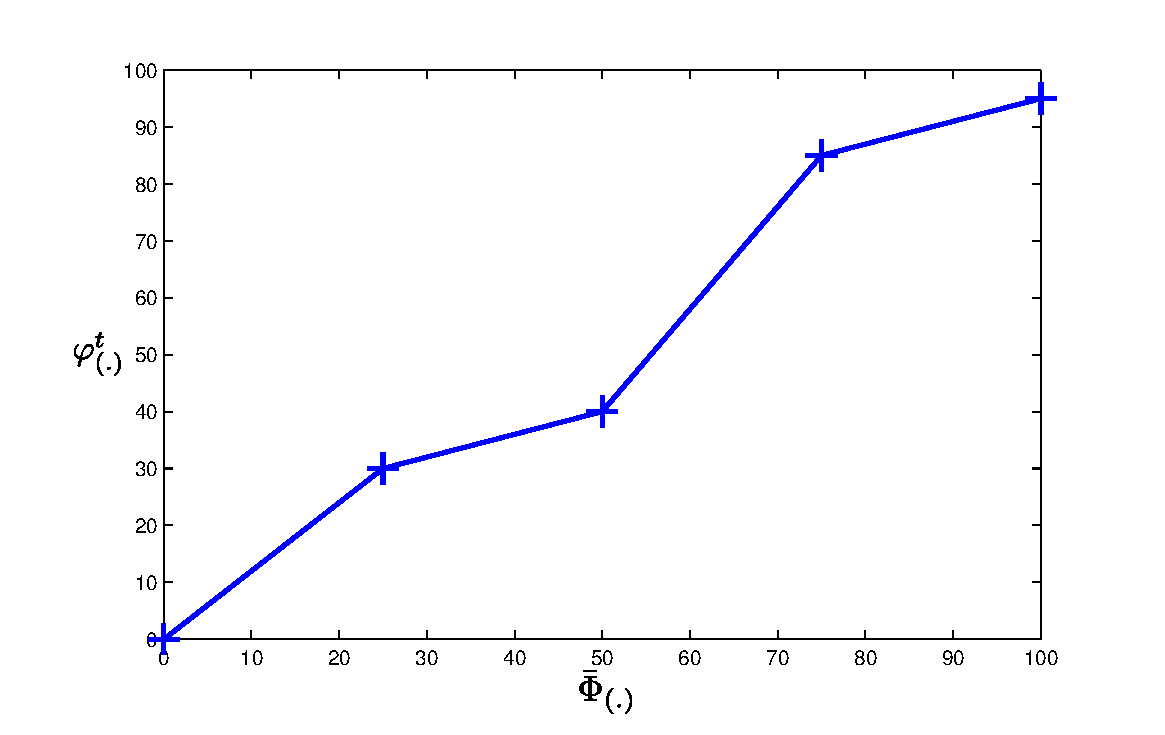
\includegraphics[width=0.9\linewidth]{03_image_processing/03_preprocessing/figures/normalization/linear_transform_parts.eps}
%	\caption{Example of linear mapping by parts as proposed by \cite{Nyul2000}.}
%	\label{fig:imnorm}
%\end{figure}
%
%Then, the mean of each quantile $\{ \bar{\Phi}_{0}, \bar{\Phi}_{25}, \bar{\Phi}_{50}, \bar{\Phi}_{75}, \bar{\Phi}_{100} \}$ is also calculated.
%Once this training stage is performed, a linear transformation by parts $\mathcal{T}(\cdot)$ can be computed (Eq. \eqref{eq:linearMap}) for each test image $t$ by mapping each statistical landmark $\varphi_{(cdot)}̂^{t}$ of this image with the pre-learned statistical landmarks $\bar{\Phi}_{(\cdot)}$. This linear mapping is also depicted in Fig.~\ref{fig:imnorm}.
%
%\begin{equation}
%\small
%\mathcal{T}(s(\mathbf{x})) =
%  \begin{cases}
%    \lceil \bar{\Phi}_{0}+( s(\mathbf{x}) - \varphi_{0}^{t} ) \left( \frac{\bar{\Phi}_{25} - \bar{\Phi}_{0}}{\varphi_{25}^{t} - \varphi_{0}^{t}} \right) \rceil \ , & \text{if $\varphi_{0}^{t} \leq s(\mathbf{x})<\varphi_{25}^{t})$} \ , \\
%    \lceil \bar{\Phi}_{25}+( s(\mathbf{x}) - \varphi_{25}^{t} ) \left( \frac{\bar{\Phi}_{50} - \bar{\Phi}_{25}}{\varphi_{50}^{t} - \varphi_{25}^{t}} \right) \rceil \ , & \text{if $\varphi_{25}^{t} \leq s(\mathbf{x})<\varphi_{50}^{t})$} \ , \\
%    \lceil \bar{\Phi}_{50}+( s(\mathbf{x}) - \varphi_{50}^{t} ) \left( \frac{\bar{\Phi}_{75} - \bar{\Phi}_{50}}{\varphi_{75}^{t} - \varphi_{50}^{t}} \right) \rceil \ , & \text{if $\varphi_{50}^{t} \leq s(\mathbf{x})<\varphi_{75}^{t})$} \ , \\
%   \lceil \bar{\Phi}_{75}+( s(\mathbf{x}) - \varphi_{75}^{t} ) \left( \frac{\bar{\Phi}_{100} - \bar{\Phi}_{75}}{\varphi_{100}^{t} - \varphi_{75}^{t}} \right) \rceil \ , & \text{if $\varphi_{75}^{t} \leq s(\mathbf{x})\leq \varphi_{100}^{t})$} \ ,
%  \end{cases}
%  \label{eq:linearMap}
%\end{equation}

\cite{Viswanath2009,Viswanath2011,Viswanath2012} used a variant of this previous approach presented in the work of \cite{Madabhushi2006a} aiming to standardize the \ac{t2w}-\ac{mri} images. Instead of computing the \ac{pdf} of an entire image, a pre-segmentation of the foreground is carried out via \ac{gscale}.% which was discussed in the bias correction section. Once the foreground is detected, the largest region is extracted and the same process than previously mentioned (see Eq. \eqref{eq:linearMap}) takes place in order to align \acp{pdf} of the foreground of the \ac{mri} images.

\begin{figure}
\centering
	\hspace*{\fill}
	\subfigure[Illustration and location of the bladder on a \ac{t2w}-\ac{mri} image acquired with a 3.0 Tesla \ac{mri} scanner]{\label{subfig:bladder} 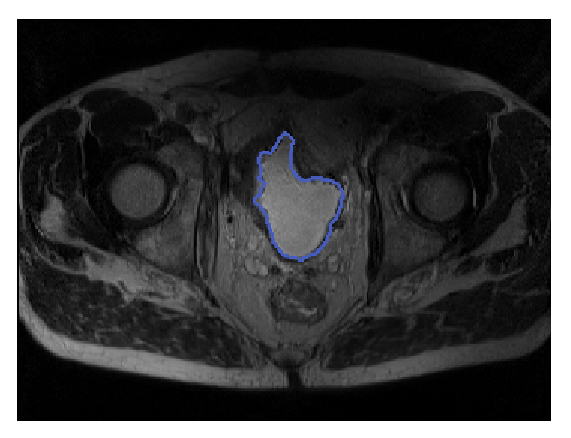
\includegraphics[width=0.4\linewidth]{03_image_processing/03_preprocessing/figures/niaf/t2w_bladder.eps}} \hfill
	\subfigure[Illustration and location of the femoral arteries on a \ac{t1w}-\ac{mri} image acquired with a 3.0 Tesla \ac{mri} scanner]{\label{subfig:arteries} \includegraphics[width=0.4\linewidth]{03_image_processing/03_preprocessing/figures/niaf/t1w_arteries.eps}}
	\hspace*{\fill}
	\caption{Illustration of the two organs used by \cite{Niaf2011,Niaf2012} to normalize \ac{t2w} and \ac{t1w} \ac{mri} images.}
	\label{fig:niaf}
\end{figure}

The methods described above were statistical-based methods. However, the standardization problem can be tackled by normalizing the MRI images using the \ac{si} of some known organs present in these images. \cite{Niaf2011,Niaf2012} normalized \ac{t2w}-\ac{mri} images by dividing the original \ac{si} of the images by the mean \ac{si} of the bladder (see Fig.~\ref{subfig:bladder}). Likewise, \cite{Niaf2011} standardized the \ac{t1w}-\ac{mri} images using the \ac{aif}. They computed the \ac{aif} by taking the mean of the \ac{si} in the most enhanced part of the common femoral arteries (see Fig.~\ref{subfig:arteries}) as proposed by \cite{Wiart2007}.

\end{enumerate}

\subsubsection{\ac{mrsi} spectra}

Presented in Sect. \ref{subsubsec:mrimrsi}, \ac{mrsi} is a modality related to a one dimensional signal. Hence, specific pre-processing steps for this type of signals have been applied instead of standard signal processing methods.

\setenumerate{listparindent=\parindent,itemsep=10px}
\setlist{noitemsep}
\begin{enumerate}[leftmargin=*]

	\item[$-$] \textbf{\textit{Phase correction:}} \ac{mrsi} data acquired suffer from zero-order and first-order phase misalignments as shown in Fig.~\ref{fig:phase} (\cite{Chen2002,Osorio-Garcia2012}). 
	
\cite{Parfait2012} used a method proposed by \cite{Chen2002} where the phase of \ac{mrsi} signal is corrected based on entropy minimization in the frequency domain.% The corrected \ac{mrsi} signal $o(\xi)$ can be expressed as:
%
%\begin{eqnarray}
%	\Re(o(\xi)) & = & \Re(s(\xi))\cos(\Phi(\xi)) - \Im(\xi)\sin(\Phi(\xi)) \ , \nonumber  \\
%	\Im(o(\xi)) & = & \Im(s(\xi))\cos(\Phi(\xi)) + \Re(\xi)\sin(\Phi(\xi)) \ , \nonumber \\
%	\Phi(\xi) & = & \phi_0 + \phi_1 \frac{\xi}{N} \ , \label{eq:mrsiphcorr}
%\end{eqnarray}
%
%\noindent where $\Re(\cdot)$ and $\Im(\cdot)$ are the real and imaginary part of the complex signal respectively, $s(\xi)$ is the corrupted \ac{mrsi} signal, $\phi_0$ and $\phi_1$ are the zero-order and first-order phase correction terms respectively and $N$ is the total number of samples of the \ac{mrsi} signal.
%
%\cite{Chen2002} tackled this problem using an optimization framework where $\phi_0$ and $\phi_1$ had to be inferred. Hence, the simplex Nelder-Mead optimization method was used to minimize the following cost function based on the Shannon entropy formulation:
%
%\begin{equation}
%	\hat{\Phi} = \argmin_{\Phi} \left[ - \sum \Re(s'(\xi)) \ln \Re(s'(\xi)) + \lambda \|\Re(s(\xi))\|_2 \right] \ ,
%	\label{eq:phcost}
%\end{equation}
%
%\noindent where $s'(\xi)$ is the first derivative of the corrupted signal $s(\xi)$ and $\lambda$ is a regularization parameter.
%
%Once the best parameter $\Phi$ is obtained, the \ac{mrsi} signal is corrected using Eq. \eqref{eq:mrsiphcorr}.

\begin{figure}
	\centering
	\includegraphics[width=0.6\linewidth]{03_image_processing/03_preprocessing/figures/phase/phase.eps}
	\caption{Illustration of frequency and phase misalignment in an \ac{mrsi} spectra acquired with a 3.0 Tesla \ac{mrsi} scanner. Focusing on the phase misalignment, note the distortion of the signal specially visible for the water (cf., around 5.1 ppm) and citrate (cf., around 3 ppm) peaks. Regarding the frequency misalignment, the water peak is known to be aligned at 4.65 ppm. However, it can observed that this peak is occurring around 5.1 ppm.}
	\label{fig:phase}
\end{figure}

	\item[$-$] \textbf{\textit{Water and lipid residuals filtering:}} The water and lipid metabolites occur in much higher concentrations than the metabolites of interests (cf., choline, creatine and citrate) (\cite{Zhu2010,Osorio-Garcia2012}). Fortunately, specific \ac{mrsi} sequences were developed in order to suppress water and lipid metabolites using pre-saturation techniques (\cite{Zhu2010}). However, these techniques do not perfectly remove water and lipids peaks and some residuals are still present in the \ac{mrsi} spectra as shown in Fig.~\ref{fig:waterfat}. Therefore, different post-processing methods have been proposed to enhance the quality of the \ac{mrsi} spectra by removing these residuals.
	
	\cite{Kelm2007} used the well known HSVD algorithm proposed by \cite{Pijnappel1992} which models the \ac{mrsi} signal by a sum of exponentially damped sinusoids in the time domain.% In the time domain, a \ac{mrsi} signal $s(t)$ is modelled by a sum of $K$ exponentially damped sinusoids such that:
%\begin{equation}
%	s(t) = \sum_{k=1}^{K} a_{k}\exp(i \phi_k) \exp( -d_{k} + i 2 \pi f_{k} ) t + \eta(t) \ ,
%	\label{eq:fidsig}
%\end{equation}
%
%\noindent where $a_k$ is the amplitude proportional to the metabolite concentration with a resonance frequency $f_{k}$, $d_k$ represents the damping factor of the exponential, $\phi_k$ is the first-order phase and $\eta(t)$ is a complex white noise. 
%
%\cite{Pijnappel1992} showed that the ``noise-free signal'' can be found using the \ac{svd} decomposition. First the noisy signal is reorganized inside a Hankel matrix $H$. It can be shown that if the signal considered would be a ``noise-free signal'', the rank of $H$ would be equal to rank $K$. However, due to the presence of noise, $H$ is in fact a full rank matrix. Thus, to recover the ``noise-free signal'', the rank of $H$ can be truncated to $K$ using its \ac{svd} decomposition. Hence, knowing the cut off frequencies of water (cf., 4.7 ppm) and lipid (cf., 2.2 ppm) metabolites, their corresponding peaks can be reconstructed and subtracted from the original signal (\cite{Laudadio2002}).

\begin{figure}
\centering
	\includegraphics[width=0.6\linewidth]{03_image_processing/03_preprocessing/figures/water/water_fat.eps}
	\caption{Illustration of the residues of water and fat even after their suppression during the acquisition protocol. The acquisition was carried out with a 3.0 Tesla \ac{mri}.}
	\label{fig:waterfat}
\end{figure}
	
\item[$-$] \textbf{\textit{Baseline correction:}} Sometimes, the problem discussed in the above section regarding the lipid molecules is not addressed simultaneously with water residuals suppression. Lipids and macromolecules are known to affect the baseline of the \ac{mrsi} spectra. They could cause errors during further fitting processes aiming to quantify the metabolites, especially regarding the citrate metabolite.
	
\cite{Parfait2012} made the comparison of two different methods to detect the baseline and correct the \ac{mrsi} spectra which are based on the work of \cite{Lieber2003} and \cite{Devos2004}. \cite{Lieber2003} addressed the problem of baseline detection in the frequency domain by iteratively fitting a polynomial of low degree.% $p(x)$ (e.g., second or third degree) to the \ac{mrsi} signal $s(x)$ in a least-squares sense. Then, the values of the fitted polynomial are re-assigned as:
%
%\begin{equation}
%	p_f(x) = 
%	\begin{cases}
%		p(x) \ , & \text{if $p(x) \leq s(x)$} \ , \\
%		s(x) \ , & \text{if $p(x) > s(x)$} \ . \\
%	\end{cases}
%	\label{eq:lieber}
%\end{equation}
%
%Finally, this procedure of fitting and re-assignment is iteratively repeated on $p_f(x)$ until a stopping criterion is reached. The final polynomial function can be subtracted from the original signal s(x) to correct it.

\cite{Parfait2012} modified this algorithm by convolving a Gaussian kernel to smooth the \ac{mrsi} signal instead of fitting a polynomial function.%, keeping the rest of the algorithm identical. 

Unlike \cite{Lieber2003}, \cite{Devos2004} proposed to correct the baseline in the time domain by multiplying the \ac{mrsi} signal by a decreasing exponential function.% as:
%\begin{equation}
%	c(t) = \exp (- \beta t) \ ,
%	\label{eq:devos}
%\end{equation}
%
%\noindent Having a typical value for $\beta$ of 0.15.

However, \cite{Parfait2012} concluded that the method proposed by \cite{Lieber2003} outperformed the one of \cite{Devos2004}. In the contemporary work of \cite{Tiwari2012}, the authors detected the baseline using a local non-linear fitting method avoiding regions with significant peaks which were detected using a experimentally parametrised signal-to-noise ratio (i.e. a value larger than 5 dB).

%\begin{figure}
%\centering
%	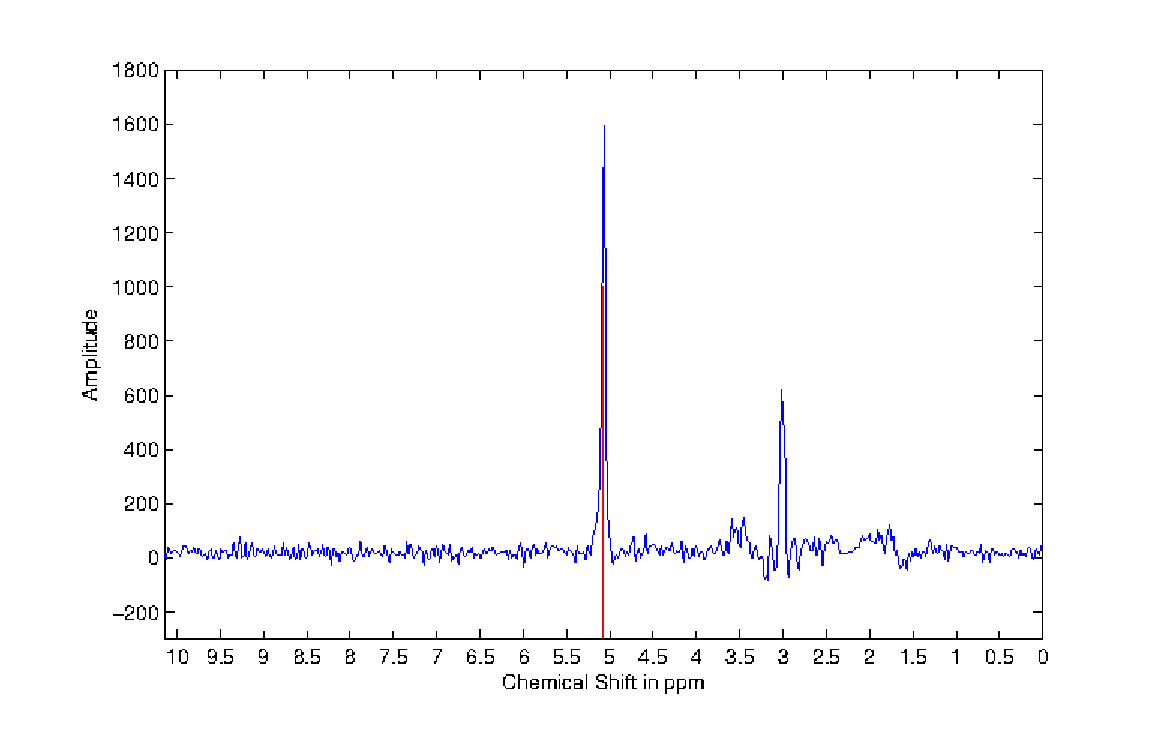
\includegraphics[width=0.9\linewidth]{03_image_processing/03_preprocessing/figures/frequency/frequency.eps}
%	\caption{Illustration of frequency misalignment in an \ac{mrsi} spectra acquired with a 3.0 Tesla \ac{mrsi} scanner. The water peak is known to be aligned at 4.65 ppm. However, it can be seen that the peak on this spectra is aligned at around 5.1 ppm.}
%	\label{fig:frequency}
%\end{figure}

	\item[$-$] \textbf{\textit{Frequency alignment:}} Due to variations of the experimental conditions, a frequency shift can be observed in the \ac{mrsi} spectra as shown in Fig.~\ref{fig:phase} (\cite{Chen2002,Osorio-Garcia2012}).
	
\cite{Tiwari2012} corrected the frequency shift by first detecting known metabolite peaks such as choline, creatine and citrate. The frequency shift is corrected by minimizing the frequency error between the experimental and theoretical values of each of these peaks.

	\item[$-$] \textbf{\textit{Normalization:}} Due to variations of the experimental conditions, the \ac{mrsi} signal may also vary between patients.
	
\cite{Parfait2012} as \cite{Devos2004} compared two methods to normalize the \ac{mrsi} signal. In each method, the original \ac{mrsi} spectra is divided by a normalization factor, similar to the intensity normalization described earlier. 

The first approach to obtain the normalization factor is based on an estimation of the water concentration. It is required to have an additional \ac{mrsi} sequence where the water metabolites are unsuppressed. Using this sequence, an estimation of the water concentration can be performed using the previously reported HSVD algorithm.  The second approach to normalization is based on using the L$_2$ norm of the \ac{mrsi} spectra $\|s(\xi)\|_2$. 
It should be noted that both \cite{Parfait2012} and \cite{Devos2004} concluded that the L$_2$ normalization was more efficient in their framework.
 
\end{enumerate}

%\def\rmm#1{{\bf \sc Robert: }{\marrow\sf #1}}


\subsection{Segmentation} \label{subsec:segmentation}

The segmentation task consists of delineating the prostate boundaries in the \ac{mri}. This procedure is of particular importance for focusing the posterior processing on the organ of interest (\cite{Ghose2012}). In this section, only the segmentation methods used in \ac{cad} systems are presented and summarized in Tab. \ref{tab:seg}. An exhaustive review of prostate segmentation methods in \ac{mri} can be found in \cite{Ghose2012} as well as prostate modelling in \cite{Chilali2014}.

\subsubsection{MRI-based segmentation}

\setenumerate{listparindent=\parindent,itemsep=10px}
\setlist{noitemsep}
\begin{enumerate}[leftmargin=*]

\item[$-$] \textbf{\textit{Manual segmentation:}} To highlight the importance of prostate segmentation task in \ac{cad} systems, it is interesting to note the large number of studies which segment manually the prostate organs (\cite{Artan2009,Artan2010,Matulewicz2013,Niaf2011,Niaf2012,Ozer2009,Ozer2010,Puech2009,Vos2008,Vos2008a}). In all the cases, the boundaries of the prostate gland are defined in order to limit the further processing to only this area. This approach ensures the right delineation of the organ nevertheless this procedure is highly time consuming and should be perform by a radiologist.

\item[$-$] \textbf{\textit{Atlas-based segmentation:}} \cite{Litjens2012} used a multi-atlas-based segmentation (\cite{Klein2008}) using multi-modal images (e.g., \ac{t2w}-\ac{mri} and \ac{adc} map) to segment the prostate with an additional pattern recognition method to differentiate \ac{cg} and \ac{pz} as proposed in \cite{Litjens2012a}. This method consists of three different steps: (i) the registration between each atlas and the multi-modal images, (ii) the atlas selection and finally (iii) the classification of the prostate segmented voxels in either \ac{cg} or \ac{pz}. 

\cite{Litjens2014} used an almost identical algorithm proposed in PROMISE12 challenge (\cite{Litjens2014a}). Their segmentation method is also based on multi-atlas multi-modal images. However, SIMPLE method (\cite{Langerak2010}) is used to combine labels after the registration of the different atlas to obtain the final segmentation.

%The registration between each atlas and the \ac{mri} images is performed using two successive registrations: the first registration is a rigid registration to roughly align the atlases and the \ac{mri} images and the second is an elastic registration using B-spline transformation. The objective function to perform the registration is defined as the weighted sum of the metric of both \ac{t2w}-\ac{mri} and \ac{adc} map. The metric is based on \ac{mi}. We refer to the next section for more details in regard to registration. Two strategies of atlas selection were performed by using either a majority voting approach or the \ac{staple} approach (\cite{Warfield2004}).
%
%Subsequently,  \ac{cg} and \ac{pz} segmentation within the prostate region is achieved by classifying each voxel using a \ac{lda} classifier. Three types of features were considered: (i) anatomy, (ii) intensity and (iii) texture. Regarding the anatomy, relative position and relative distance from the pixel to the border of the prostate were used. The intensity features consist of the intensity of the voxel in the ADC coefficient and the T$_2$ map. The texture features were composed of five different features: homogeneity, correlation (\cite{Amadasun1989}), entropy, texture strength (\cite{Li2005a}) and \ac{lbp} (\cite{Ojala1996}). Finally, morphological operations were applied to remove artefacts and the contours between the zones were smoothed using \ac{tps} (\cite{Bookstein1989}).

\item[$-$] \textbf{\textit{Model-based segmentation:}} \cite{Viswanath2008a,Viswanath2009} used the \ac{mantra} method as proposed by \cite{Toth2008}. \ac{mantra} is closely related to the \ac{asm} from \cite{Cootes1995}. This algorithm consists of two stages: (i) a training stage where a shape and appearance model is generated and (ii) the actual segmentation performed based on the learned model. 

%For the training stage, a set of landmarks is defined and the shape model is generated as in the original \ac{asm} method (\cite{Cootes1995}). Then, to model the appearance, a set of $K$ texture images $\{I_1,I_2,\cdots,I_k\}$ based on first and second order statistical texture features are computed. For a given landmark $l$ with its given neighbourhood $\mathcal{N}(l)$, its feature matrix extracted can be expressed as:
%
%\begin{equation}
%	f_l = \{ I_1(\mathcal{N}(l)), I_2(\mathcal{N}(l)), \cdots, I_k(\mathcal{N}(l)) \} \ .	
%	\label{eq:mantra1}
%\end{equation}
%
%\noindent where $I_k(\mathcal{N}(l))$ represents a feature vector obtained by sampling the $k^{\text{th}}$ texture map using the neighbourhood $\mathcal{N}(l)$.
%
%By generating multiple landmarks in the same fashion as \ac{asm}, \ac{pca} (\cite{Pearson1901}) is applied to learn the appearance variations. 
%
%For the segmentation stage, the mean shape learned previously is initialised in the test image. The same associated texture images as in the training stage are computed. For each landmark $l$, a neighbourhood of patches are used to sample the texture images and a reconstruction is obtained using the appearance model previously trained. The new landmark location will be defined as the position where the \ac{mi} is maximal between the reconstructed and original values. This scheme is performed in a multi-resolution manner as in \cite{Cootes1995}.
%
%Subsequently, the same authors (\cite{Viswanath2012}) used the \ac{weritas} method also proposed by \cite{Toth2009}. As with the \ac{mantra} method, \ac{weritas} is based on the \ac{asm} formulation. In fact it is very close to the \ac{mantra} itself. The same texture features are used to construct the appearance models, but instead of using \ac{mi} between the landmarks and neighbour patches for adapting the landmark positions, it defines a metric based on the Mahalanobis distance. In the training stage, the Mahalanobis distance is computed between landmarks and neighbour patches for each of the features. Subsequently, a new metric is proposed as a linear weighted combination of those Mahalanobis distances which maximises the correlation with the Euclidean distance between the patches and the true landmarks. In the segmentation step, this metric is then computed between the initialised landmarks and neighbouring patches in order to update landmark positions, in a similar fashion to other \ac{acm} models. 

\cite{Litjens2011} and \cite{Vos2012} used an approach proposed by \cite{Huisman2010} in which the bladder, prostate and rectum are segmented.The segmentation task is performed as an optimization problem taking into account three parameters into account linked to organs such as: (i) the shape, (ii) the location and (iii) the respective angles between them. % A probabilistic model is first trained by embedding the three following aspects: (i) the shape by defining each organ as an ellipse, (ii) the position by defining the distance and the angle between each organ center and (iii) the appearance using the \acp{pdf} of \ac{si} of each organ. 
Furthermore, \cite{Litjens2011} used only \ac{adc} map to encode the appearance whereas \cite{Vos2012} used both \ac{adc} and T$_2$ maps.% Then, during the optimization using a quasi-Newton optimizer, an objective function is minimized. This function is defined as the sum of the deviations from the above model learnt. This rough segmentation is then used inside a Bayesian framework to refine the segmentation.

\end{enumerate}

\subsubsection{MRSI-based segmentation}

\cite{Tiwari2009} localized the voxels corresponding to the prostate organ using a hierarchical spectral clustering. First, each \ac{mrsi} spectrum is projected into a lower dimension space using graph embedding (\cite{Shi2000}).% To proceed, a similarity matrix $W$ is computed using a Gaussian similarity measure from the Euclidean distance (\cite{Belkin2001}) such that:
%
%\begin{equation}
%	W(\mathbf{x},\mathbf{y}) =
%	\begin{cases}	
%	 	\exp \left( \frac{\| s(\mathbf{x}) - s(\mathbf{y}) \|_2^2}{\sigma^2} \right) \ , & \text{if } \| \mathbf{x} - \mathbf{y} \|_2 < \epsilon \ , \\
%	 	0 \ , & \text{if } \| \mathbf{x} - \mathbf{y} \|_2 > \epsilon \ .
%	 \end{cases}
%	\label{eq:ge1}
%\end{equation}
%
%\noindent where $s(\mathbf{x})$ and $s(\mathbf{y})$ are the \ac{mrsi} spectra for the voxels $\mathbf{x}$ and $\mathbf{y}$ respectively, $\sigma$ is the standard deviation of the Gaussian similarity measure and $\epsilon$ is a parameter used to define an $\epsilon$-neighbourhood.
%
%The \ac{mrsi} spectra projection into the lower dimension space is approached as a generalized eigenvector problem. Subsequently, a replicate k-means clustering method is run defining two clusters. The data corresponding to larger cluster is assumed to belong to the non-prostate voxels and these voxels will be eliminated from the processing. The full procedure is repeated until the total number of voxels left is inferior to a given threshold set experimentally.

\subsection{Registration} \label{subsec:registration}

The role of image registration is vital in \ac{cad} systems using multi-parametric \ac{mri} images. As it will be discussed in \ac{sec}\,\ref{sec:dataclassfra}, for the sake of an optimal classification, the features detected in each modality will be grouped depending of their spatial locations. Hence, one has to ensure the perfect alignment of the multi-modal \ac{mri} images ahead of performing any classification scheme.

Image registration is the procedure consisting of aligning an unregistered image (also called moving image) into a template image (also called fixed image) via a geometric transformation. This problem is usually addressed as presented in \ac{fig}\,\ref{fig:frareg}. An iterative procedure takes place to infer the geometric transformation (parametric or non-parametric) via an optimizer, which maximizes the similarity between the two images.

From \ac{sec}\,\ref{subsubsec:geotra} to \ac{sec}\,\ref{subsubsec:int}, we individually review the different components of a typical registration framework (see \ac{fig}\,\ref{fig:frareg}). \Acl{sec}~\ref{subsubsec:regrev} will summarize the combinations of these components especially for the frameworks used in \ac{cad} systems. Exhaustive reviews covering all registration methods in computer science and medical fields can be found in~\cite{Maintz1998,Zitova2003}, respectively.

\subsubsection{Geometric transformation models}\label{subsubsec:geotra}

As previously mentioned, the registration problem is to align two images or volumes by finding the geometric transformation. Regarding the transformation, from all \ac{cad} for \ac{cap} systems reviewed, only parametric methods have been implemented. Two different groups of parametric transformation models have been used, each of them are characterized by the degree of freedom that they offer.

Affine transformations provide four degrees of freedom managing rotations and translation as with the rigid transformations but also shearing and scaling. The other group of transformations is known as elastic transformations and offer the advantage to handle local distortions. In the reviewed \ac{cad} for \ac{cap} systems, the radial basis functions are used to formalize the local distortions. Two radial basis functions have been used: (i) the \ac{tps} and (ii) the B-splines. Apart from the formalism, these two approaches have a main difference. With B-splines, the control points are usually uniformly and densely placed on a grid where as with \ac{tps}, the control points correspond to detected or selected key points. By using \ac{tps}, Mitra et al. in~\cite{Mitra2011} obtained more accurate and time efficient results than with the B-splines strategy~\cite{Mitra2012a}.

It is reasonable to point out that usually only rigid or affine registrations have been used to register multi-parametric images from a same protocol. Elastic registration methods are more commonly used to register multi-protocol images (e.g., histopathology with \ac{mri} images)~\cite{Toth2008,Toth2009}.

\subsubsection{Similarity measure}\label{subsubsec:simmea}

During the registration procedure, a similarity criterion is computed in order to evaluate the quality of the alignment performed. Roughly speaking, this criterion will give the direction to take to the optimizer, in order to assign the most optimal values to the geometric transformation parameters.

The most naive similarity measure is the \acf{mse} of the \ac{si} of \ac{mri} images. However, this metric is not well suited when multi-parametric images are involved due to the tissue appearance variations between the different modalities.

In that regard, \ac{mi} was introduced as a registration measure in the late 1990's in~\cite{Pluim2003}. The \ac{mi} measure finds its foundation in the assumption that a homogeneous region in the first modality image should also appear as a homogeneous region in the second modality even if their \acp{si} are not identical. Thus, those regions share information and the registration task can be achieved by maximizing this common information. Maximizing the \ac{mi} is in fact equivalent to minimizing the joint entropy which is a measure related with the degree of uncertainty or dispersion of the data in the joint histogram. A generalized form of \ac{mi}, \ac{cmi}, was proposed in~\cite{Chappelow2011}. \ac{cmi} encompasses interdependent information such as texture and gradient into the metric.

\subsubsection{Optimization methods}\label{subsubsec:optmea}

Registration is usually regarded as an optimization problem where the parameters of the geometric transformation model have to be inferred by minimizing the similarity measure. Iterative estimation methods are commonly used: L-BFGS-B quasi-Newton method~\cite{Byrd1995} and gradient descent~\cite{Viola1997}. During our review, we noticed that authors do not usually linger over optimizer choice.

\subsubsection{Interpolation}\label{subsubsec:int}

The registration procedure involves transforming an image, and pixels mapped to non-integer points must be approximated using interpolation methods. As for the optimization methods, we notice that little attention has been paid on the choice of those interpolations methods. However, commonly used methods are bilinear, nearest-neighbour, bi-cubic, spline and inverse-distance weighting method~\cite{Mitra2012}.

\subsubsection{Review of the methods used in \ac{cad} system}\label{subsubsec:regrev}

Studies presenting a \ac{cad} pipeline incorporating an automatic registration procedure are summarized in \ac{tab}~\ref{tab:regtab}. 

Ampeliotis et al. in~\cite{Ampeliotis2007,Ampeliotis2008} did not use the framework as presented in \ac{fig}\,\ref{fig:frareg} to register 2D \ac{t2w} and \ac{dce} images. By using image symmetries and the \ac{mse} metric, they found the parameters of an affine transformation but without using a common objective function. They were finding independently and consecutively the scale factor, the rotation and finally the translation.

Giannini et al.~\cite{Giannini2013} used also a in-house development registration method to register 2D \ac{t2w} and \ac{dw} images using an affine model. The bladder is first segmented in both modalities in order to obtain its contours and to focus the registration.

Giannini et al.~\cite{Giannini2013} and also Vos et al.~\cite{Vos2010} used the same framework which is based on finding an affine transformation to register the \ac{t2w} and \ac{dce} images using \ac{mi}~\cite{Rueckert1999}. Then, an elastic registration using B-spline takes place using the affine parameters to initialize the geometric model with the  same similarity measure. However, the approaches differ regarding the choice of the optimizer since a gradient descent is used in~\cite{Giannini2013} and the same optimization problem is tackled via a quasi-Newton method in~\cite{Vos2010}. Moreover, Giannini et al.~\cite{Giannini2013} performed a 2D registration whereas Vos et al.~\cite{Vos2010} registered 3D volumes.

Viswanath et al. in~\cite{Viswanath2008a,Viswanath2009} as well as Vos et al.~\cite{Vos2008} performed an affine registration using the \ac{mi} as similarity measure to correct the misalignment between \ac{t2w} and \ac{dce} images. The choice of the optimizer was not specified. Viswanath et al.~\cite{Viswanath2008a,Viswanath2009} focused on 2D registration while Vos et al.~\cite{Vos2008} performed 3D registration.

Finally, Viswanath et al. in~\cite{Viswanath2011} performed a 3D registration with the three modalities, \ac{t2w} and \ac{dce} and \ac{dw} \ac{mri}, by using an affine transformation model combined with the \ac{cmi} similarity measure as presented in~\cite{Chappelow2011}. Moreover, in this latter work, the authors employed a gradient descent approach to solve this problem but suggested Nelder-Mead simplex and quasi-Newton method as other solutions.

%%% Local Variables: 
%%% mode: latex
%%% TeX-master: "../../g_lemaitre_state_of_the_art"
%%% End: 


\section{\ac{cade} - \ac{cadx}} \label{sec:dataclassfra}

\subsection{\ac{cade}: \acp{roi} detection/selection}\label{cade}

As discussed in the introduction and shown in \ac{fig}\,\ref{fig:wkfcad}, the image classification framework is often composed of a \ac{cade} and a \ac{cadx}. In this section, we will focus on studies embedding a \ac{cade} in their framework. Two approaches are considered to define a \ac{cade} (see \ac{tab}~\ref{tab:cade}): (i) voxel-based delineation and (ii) lesion segmentation.
The first strategy, which concerns the majority of the studies reviewed (see \ac{tab}~\ref{tab:cade}), is in fact linked to the nature of the classification framework. All voxels are considered as a possible lesion and the output of the framework will be pixels classified as lesion and non lesion.\robert{there are no works commented in the text on this first group? why?}
The second group of methods is composed of method implementing a lesion segmentation algorithm to delineate potential candidates to further obtain a diagnosis through the \ac{cadx}. This approach was borrowed from other application areas such as breast cancer. These methods are in fact very similar to the classification framework used in \ac{cadx} later.

Vos et al.~\cite{Vos2012} highlighted lesion candidates by detecting blobs in the \ac{adc} map. These candidates were filtered using some \textit{a priori} criteria such as \ac{si} or diameter. The candidate blobs detected are then filtered depending on their appearances (cf. maximum of the likelihood of the region, diameter of the lesion) and their \ac{si} in \ac{adc} and \ac{t2w} images. The detected regions are then used as inputs for the \ac{cadx}.

Litjens et al.~\cite{Litjens2011} used a pattern recognition approach in order to delineate the \acp{roi}. A blobness map was calculated in the same manner as previously in~\cite{Vos2010} using the multi-resolution Hessian blob detector on the \ac{adc} map, \ac{t2w} and pharmacokinetic parameters maps (see \ac{sec}\,\ref{subsec:featuredetection} for details about those parameters). Additionally, the position of the voxel $\mathbf{x}=\{x,y,z\}$ was used as a feature as well as the Euclidean distance of the voxel to the prostate center. Hence, the feature vectors were composed of eight features and a \ac{svm} classifier was trained using a \ac{rbf} kernel (see \ac{sec}\,\ref{subsec:classification} for more details).

Subsequently, Litjens et al. in~\cite{Litjens2012} modified this approach by including only features related to the blob detection on the different maps as well as the original \acp{si} of the parametric images. Two new maps were introduced based on texture. Instead of a \ac{svm} classifier, a \ac{knn} classifier was used. The candidate regions were then extracted by performing a local maxima detection followed by post-processing region-growing and morphological operations. 

In a similar way, Litjens et al. in~\cite{Litjens2014} used the same approach and added two new features: (i) a Gaussian texture bank on \ac{t2w} to create new maps and (ii) the \ac{dw} \ac{mri} image acquired with $b=800$ s.mm$^-2$. Three classifiers were tested: \ac{lda}, GentleBoost and Random forest. After evaluation, random forest was selected as classifier due to its overall performances.

%%% Local Variables: 
%%% mode: latex
%%% TeX-master: "../../g_lemaitre_state_of_the_art"
%%% End: 

\subsection{\ac{cadx}: Feature detection} \label{subsec:featuredetection}

Discriminative features which can be used to recognize \ac{cap} from healthy tissue have to be first detected. This processing is known in computer vision as feature extraction. However, feature extraction is also the name given in pattern recognition to some types of dimension reduction methods which will be presented in the next section. In order to avoid confusion between these two aspects, in this survey, the procedure ``detecting'' or ``extracting'' features from images and signals will be defined as feature detection. This section will summarize the different strategies employed for this task. The features used in the studies reviewed are summarized in Tab. \ref{tab:feat}.

\subsubsection{Image-based features}

This section will focus on image-based features detection. Two main strategies to detect features have been identified and used for the purpose of our classification: (i) voxel-wise detection and (ii) region-wise detection.

\setenumerate{listparindent=\parindent,itemsep=10px}
\setlist{noitemsep}
\begin{enumerate}[leftmargin=*]

\item[$-$] \textbf{\textit{Voxel-wise features:}} This strategy refers to the fact that a feature is extracted at each voxel location of an image.

  \ac{cap} as previously discussed (see Tab. \ref{tab:modmri}) can be discerned due to \ac{si} changes. Hence, intensity-based features are one of the most common features used to build the feature vector which has to be classified (\cite{Ampeliotis2007,Ampeliotis2008,Artan2009,Artan2010,Chan2003,Langer2009,Litjens2011,Litjens2012,Litjens2014,Liu2009,Niaf2011,Niaf2012,Viswanath2008a,Viswanath2011}). This type of feature consists simply of the \ac{si} of each voxel of the different \ac{mri} modalities.

  \Ac{si} changes can be viewed as heterogeneous regions and edge-based features are used in that regard. Each feature is computed by convolving the original image with an edge operator. Three of these operators are used in \ac{cad} systems: (i) Prewitt operator (\cite{Prewitt1970}), (ii) Sobel operator (\cite{Sobel1970}) and (iii) Kirsch operator (\cite{Kirsch1971}). Results obtained with these operators vary, due to their different kernels. These features are commonly incorporated in the feature vector for further classification in the \ac{cad} systems reviewed (\cite{Niaf2011,Niaf2012,Tiwari2009a,Tiwari2010,Tiwari2013,Viswanath2008,Viswanath2011}).

  Gabor filters (\cite{Gabor1946,Daugman1985}) offer another approach to extract information related to edges and texture. \cite{Viswanath2008a,Viswanath2012} and \cite{Tiwari2012} integrated Gabor analysis in their feature vector.

  Texture-based features provide other characteristics discerning \ac{cap} from healthy tissue. The most common texture analysis for image classification are co-occurrence matrices with their related statistics which were proposed by \cite{Haralick1973} and are commonly used in \ac{cad} systems (\cite{Antic2013,Niaf2011,Niaf2012,Tiwari2009a,Tiwari2010,Tiwari2013,Viswanath2008,Viswanath2008a,Viswanath2011,Viswanath2012}).

  Fractal analysis and more precisely a local estimation of the fractal dimension (\cite{Benassi1998}) describing the texture roughness at a specific location was used in \cite{Lopes2011}. A wavelet-based method in a multi-resolution framework was used to estimate the fractal dimension. Cancerous tissue were characterized to have a higher fractal dimension than healthy tissue.

  \cite{Chan2003} aimed to describe the texture using the frequency signature via the \acf{dct} (\cite{Ahmed1974}) defining a neighbourhood of $7 \times 7$ pixels for each of the modalities that they used.

  In the same spirit, \cite{Viswanath2012} projected \ac{t2w} images into the wavelet space and used the coefficients obtained from the decomposition as features. The wavelet family used for the decomposition was the Haar wavelet.

  \cite{Litjens2014} compute texture map based on \ac{t2w} images using a Gaussian filter bank (\cite{Leung2001}).

  The position of a voxel within the prostate was also considered a possible feature. \cite{Litjens2011,Litjens2014} computed the Euclidean distance from each voxel to the prostate center as well as the individual distance in the three directions $x$, $y$ and $z$. \cite{Chan2003} embedded the same information but this time using cylindrical coordinates $r$, $\theta$ and $z$ corresponding to the radius, azimuth and elevation respectively.

\item[$-$] \textbf{\textit{Region-wise features:}}

  Unlike the previous section, another strategy is to study an entire region and extract characteristic features corresponding to this region.

  The most common approach reviewed can be classified as statistical methods. First, a feature map are computed for the whole image and not any more for a single voxel. Then, \acp{roi} are defined and statistics are extracted from each of these regions. The first type of statistic is based on percentiles and is widely used (\cite{Antic2013,Litjens2011,Litjens2012,Litjens2014,Peng2013,Tiwari2009a,Tiwari2010,Tiwari2013,Viswanath2008,Viswanath2008a,Viswanath2011,Viswanath2012,Vos2008,Vos2008a,Vos2010,Vos2012}). In fact, once that a \ac{roi} is defined, the features corresponding to the $n^{\text{th}}$ percentile are used as feature. This $n$ can take any value between $0$ and $100$. This threshold is usually manually determined observing the distribution and corresponds to the best discriminant value differentiating malignant and healthy tissue. in addition, statistic-moments such as mean, standard deviation, kurtosis and skewness are also used (\cite{Ampeliotis2007,Ampeliotis2008,Antic2013,Niaf2011,Niaf2012,Peng2013}). \cite{Litjens2014} also introduced a feature based on symmetry. They compute the mean of a candidate lesion as well as its mirrored counter-part and compute the quotient as feature.

  Another subset of features are anatomic which were also used by \cite{Litjens2012,Litjens2014} and \cite{Matulewicz2013}. \cite{Litjens2012,Litjens2014} computed the volume, compactness and sphericity related to the region to integrate it in their feature vector to later classify. \cite{Matulewicz2013} introduced four features corresponding to the percentage of tissue belonging to the regions \ac{pz}, \ac{cg}, periurethral region or outside prostate region for the considered \ac{roi}.

  In contrast to anatomical are histogram-based feature descriptors. For instance, \cite{Liu2013} introduced four different types of histogram-based features. The first type corresponds to the histogram of the \ac{si} of the image. The second type is the \acf{hog} (\cite{Dalal2005}). \Ac{hog} descriptor describes the local shape of the object of interest by using gradient directions distribution. The third histogram-based type used by \cite{Liu2013} was shape context (\cite{Belongie2002}). The shape context is also a way to describe the shape of an object of interest. The last set of histogram-based feature extracted is based on the framework of \cite{Zhao2012} which is using the Fourier transform of the histogram created via \acf{lbp} (\cite{Ojala1996}).

  The last group of region-based feature is based on fractal analysis. The features proposed are based on estimating the fractal dimension which is a statistical index representing the complexity of what is analysed. \cite{Lv2009} proposed two features based on fractal dimension: (i) texture fractal dimension and (ii) histogram fractal dimension. \cite{Lopes2011} proposed a 3D version to estimate the fractal dimension of a volume using wavelet decomposition.
\end{enumerate}

\subsubsection{\ac{dce}-based features}\label{subsubsec:fddce}

\ac{dce}-\ac{mri} is more commonly based on a \ac{si} analysis over time as presented in Sect. \ref{subsubsec:mrimrsi}. The parameters extracted used in \ac{cad} system during the \ac{dce}-\ac{mri} analysis are presented.

\setenumerate{listparindent=\parindent,itemsep=10px}
\setlist{noitemsep}
\begin{enumerate}[leftmargin=*]

\item[$-$] \textbf{\textit{Whole-spectra approach:}} Some studies are using the whole \ac{dce} time series as feature vector such as \cite{Ampeliotis2007,Ampeliotis2008}, \cite{Tiwari2012} and \cite{Viswanath2008a,Viswanath2008}. In some cases, the high-dimensional feature space is reduced using dimension reduction methods as it will be presented in the next section (see Sect. \ref{subsec:featureselectionextraction}).

\item[$-$] \textbf{\textit{Semi-quantitative approach:}} Semi-quantitative approaches are based on mathematically modelling the \ac{dce} time series. The parameters modelling the signal are commonly used mainly due to the simplicity of their computation. Parameters included in semi-quantitative analysis are summarized in Tab. \ref{tab:semiqua} and also graphically depicted in Fig.~\ref{fig:dceparam}. A set of time features corresponding to specific amplitude level (start, maximum and end) are extracted. Then, derivative and integral features are also considered as discriminative and are commonly computed.

\item[$-$] \textbf{\textit{Quantitative approach:}} As presented in Sect. \ref{subsubsec:mrimrsi}, quantitative approaches correspond to mathematical-pharmacokinetic models based on physiological exchanges. Four different models have been used in \ac{cad} systems. The most common model reviewed was the Brix model using three parameters $A$, $k_{ep}$ and $k_{el}$ (\cite{Artan2009,Artan2010,Sung2011,Liu2009,Ozer2009,Ozer2010}). The Tofts model and more precisely the parameters $K_{trans}$, $k_{ep}$ and $v_e$ (\cite{Tofts1997}) was used by \cite{Langer2009,Litjens2011,Litjens2012,Litjens2014,Giannini2013,Niaf2011,Niaf2012,Mazzetti2011}.

  \cite{Mazzetti2011} and \cite{Giannini2013} used the Weibull function defined by two parameters. They also used another empirical model which is based on the West-like function and named the phenomenological universalities model (\cite{Castorina2006}) using the three parameters the parameters $\beta$, $a_0$ and $r$.

  For all these models, the parameters are inferred using an optimization curve fitting approach.

\end{enumerate}

\subsubsection{\ac{mrsi}-based features}

\setenumerate{listparindent=\parindent,itemsep=10px}
\setlist{noitemsep}
\begin{enumerate}[leftmargin=*]

\item[$-$] \textbf{\textit{Whole spectra approach:}} As in the case of \ac{dce} analysis, one common approach is to incorporate the whole \ac{mrsi} spectra in the feature vector for classification (\cite{Kelm2007,Parfait2012,Tiwari2007,Tiwari2009,Tiwari2013,Tiwari2009a,Tiwari2010,Viswanath2008a,Matulewicz2013}). Sometimes post-processing involving dimension reduction methods is performed to reduce the complexity during the classification as it will be presented in Sect. \ref{subsec:featureselectionextraction}.

\item[$-$] \textbf{\textit{Quantification approach:}} We can reiterate that in \ac{mrsi} only few biological markers (cf., choline, creatine and citrate metabolites mainly) are known to be useful to discriminate \ac{cap} and healthy tissue. Then, concentrations of these metabolites can be considered as a feature used for classification. In order to perform this quantification, four different approaches have been used. The QUEST (\cite{Ratiney2005}), AMARES (\cite{Vanhamme1997}) and VARPRO (\cite{Coleman1993}) models were used by \cite{Kelm2007}. They are all time-domain quantification methods varying by the type of pre-knowledge embedded and the optimization approaches used to solve the quantification problem. Unlike the time-domain quantification approaches, \cite{Parfait2012} used the LcModel approach (\cite{Provencher1993}) which solves the optimization problem in the frequency domain.

  Once the different concentrations are computed, \cite{Kelm2007} calculated the relative concentrations (Eq. \eqref{eq:ratio1} and \eqref{eq:ratio2}) and used them as features. However, \cite{Parfait2012} used each metabolite concentrations individually.

  \begin{eqnarray}
    R_1 & = & \frac{ [ \text{Cho} ] + [ \text{Cr} ]}{[ \text{Cit} ]} \ . \label{eq:ratio1} \\
    R_2 & = & \frac{[ \text{Cit} ]}{[\text{Cho}]+[\text{Cr}]+[\text{Cit}]} \ , \label{eq:ratio2}
  \end{eqnarray}

  \noindent where $\text{Cit}$, $\text{Cho}$ and $\text{Cr}$ are the concentration of citrate, choline and creatine respectively.

\item[$-$] \textbf{\textit{Wavelet decomposition approach:}} \cite{Tiwari2012} performed a wavelet packet decomposition (\cite{Coifman1992}) with the Haar wavelet basis function and used the coefficients of this decomposition as features for further classification.

\end{enumerate}

%%% Local Variables: 
%%% mode: latex
%%% TeX-master: "../../g_lemaitre_state_of_the_art"
%%% End: 

\subsection{Feature selection and feature extraction} \label{subsec:featureselectionextraction}

As presented in the previous section, a wide variety of features can be computed (see Tab. \ref{tab:feat}). Using multi-parametric data as well as multiple features lead to a high complexity feature space which might mislead or corrupt the classifier which have to be trained. Thus, one will be interesting to reduce the number of dimension of the feature space before to proceed to any classification task. The strategy used can be group into two groups: (i) feature selection and (ii) feature extraction. The methods used for \ac{cad} system are summarized in Tab. \ref{tab:featext}.

\subsubsection{Feature selection}\label{subsubsec:featsel}

The feature selection strategy corresponds in selecting the most discriminative feature dimension of the high-dimensional space. Thus, the low-dimensional space is then composed of a subset of the original features detected. In this section, methods employed in the studies reviewed will be briefly presented. More extensive review specific to feature selection can be found in \cite{Saeys2007}.

\cite{Niaf2011,Niaf2012} make use of the p-value by using the independent two-sample t-test with equal mean for each feature dimension. In this statistical test, it is assumed two classes, \ac{cap} against healthy. Hence, for each particular feature, the distribution of each class can be characterized by their means $\bar{X}_1$ and $\bar{X}_2$ and standard deviation $s_{X_1}$ and $s_{X_2}$, respectively. Hence, the null hypothesis tested is based on the fact that these both distribution means are equal. Thus, the t-statistic related to verify the null hypothesis is then formalized such that:

\begin{eqnarray}
t & = & \frac{\bar {X}_1 - \bar{X}_2}{s_{X_1X_2} \cdot \sqrt{\frac{1}{n_1}+\frac{1}{n_2}}} \ , \label{eq:tstat} \\
s_{X_1X_2} & = & \sqrt{\frac{(n_1-1)s_{X_1}^2+(n_2-1)s_{X_2}^2}{n_1+n_2-2}} \ , \nonumber
\end{eqnarray}

\noindent where $n_1$ and $n_2$ are the number of sample in each class.

\begin{table}
	\caption{Overview of the feature selection and extraction methods used in \ac{cad} systems.}
	\small
	%\renewcommand{\arraystretch}{1.5}
	\begin{tabular}{p{.65\linewidth} p{.25\linewidth}}
		\hline \\ [-1.5ex]
		\textbf{Dimension reduction methods} & \textbf{References} \\ \\ [-1.5ex]
		\hline \\ [-1.5ex]
		\textit{Feature selection:} & \\ \\ [-1.5ex]
		\quad Statistical test & $[$17-18,41$]$ \\
		\quad \ac{mi}-based methods & $[$18-19,37$]$ \\ \\ [-1.5ex]
		\textit{Feature extraction:} & \\ \\ [-1.5ex]
		\quad Linear mapping & \\
		\quad \quad \acs{pca} & $[$27-28,31$]$ \\
		\quad Non-linear mapping & \\
		\quad \quad Laplacian eigenmaps & $[$26,28-30,33,36$]$ \\
		\quad \quad \acs{lle} and \acs{lle}-based & $[$27-28,33-34$]$ \\ \\ [-1.5ex]
		\hline
	\end{tabular}
	\label{tab:featext}
\end{table}

From Eq. \eqref{eq:tstat}, it can be seen that the more the means of the class distribution diverge, larger the $t$-statistic $t$ will be implying that this particular feature is more relevant and able to make the distinction between the two classes to separate. 

The $p$-value statistic can be deduced from the $t$-test and corresponds to the probability to obtain such an extreme test assuming that the null hypothesis is true \cite{Goodman1999}. Hence, smaller is the $p$-value, more likely is to reject the null hypothesis and more relevant the feature is likely to be.

Finally, the feature can be ranked and the most significant features can be selected, by defining the number of features wanted. However, this technique suffers from a main drawback since that it is assumed that each feature are independent which is unlikely to happen and introduce a high redundancy in the feature selected.

\cite{Vos2012} employed a similar feature ranking approach but make use of the Fisher discriminant ratio to compute the relevance of each feature dimension. Taking the aforementioned formulation, the Fisher discriminant ratio is formalized as the ratio of the variance between classes to the variance within classes such that:

\begin{equation}
F_r = \frac{\bar{X}_1 - \bar{X}_2}{s^{2}_{X_1}+s^{2}_{X_2}} \ .
\label{eq:fisherratio}
\end{equation}

Hence, a feature dimension can be seen as more relevant when the variance between classes is maximum and the variance within classes in minimum. Once the features ordered, \cite{Vos2012} select the feature dimensions with the larger Fisher discriminant ratio.

\ac{mi} can also be used to select the subset of feature dimension. Definition of the \ac{mi} was presented in Sect. \ref{subsubsec:simmea} and formalized in \eqref{eq:midef}. The computation of the entropies involves the estimation of some \acp{pdf} and the data being usually continuous variables, it is then necessary to estimate the \acp{pdf} using method such as Parzen windows.

\cite{Peng2005} introduced two main criteria to select the features dimensions and then combined: (i) maximal relevance and (ii) minimum redundancy.

Maximal relevance criterion is based on the paradigm that the classes and the feature dimension which have to be selected have to share a maximal \ac{mi} and can be formalized such that:

\begin{eqnarray}
	&&\argmax Rel(\mathbf{x},c) \ , \nonumber \\
	&& Rel(\mathbf{x},c) = \frac{1}{|\mathbf{x}|} \sum_{x_i \in \mathbf{x}} MI(x_i,c)  \ , \label{eq:mRel}
\end{eqnarray}

\noindent where $\mathbf{x} = \{x_i,i=1,\cdots,d\}$ is a feature vector of $d$ dimensions, $c$ is the class considered and $MI(\cdot)$ is the \ac{mi}.

As in the previous method, using maximal relevance criterion alone will imply the independence between each feature dimension which is usually not true.

Minimal redundancy criterion will force to select a new feature dimension which shares as less as possible \ac{mi} with previously selected feature dimension. It can be formalized as:

\begin{eqnarray}
	&&\argmin Red(\mathbf{x}) \ , \nonumber \\
	&& Red(\mathbf{x}) = \frac{1}{|\mathbf{x}|^2} \sum_{x_i,x_j \in \mathbf{x}} MI(x_i,x_j)  \ . \label{eq:mRed}
\end{eqnarray}

Combination of these two previous criteria is known as \ac{mrmr}\footnote{\ac{mrmr} implementation can be found at: \texttt{http://penglab.janelia.\allowbreak org/proj/mRMR/}} (\cite{Peng2005}) and can be computed such as a difference or a quotient of the Eq. \eqref{eq:mRel} and \eqref{eq:mRed}.

\cite{Niaf2011,Niaf2012} make use of maximal relevance criterion alone and also of both \ac{mrmr} difference and quotient criterion. \cite{Viswanath2012} also reduced their feature vector via \ac{mrmr} difference and quotient.

\subsubsection{Feature extraction}

The feature extraction strategy is related to dimension reduction methods and are not selecting discriminative features. Instead, these methods aimed at mapping the data from the high-dimensional space into a low-dimensional space created to maximize the separability between the classes. The mapping can be performed from a linear or a non-linear manner. Only methods employed in \ac{cad} system will be reviewed in this section. We guide the reader to the review of \cite{Fodor2002} for a full review of feature extraction techniques.

Linear mapping method used to reduce the dimensionality in \ac{cad} system is usually the \ac{pca}. 

\ac{pca} is a method allowing to find the orthogonal linear transform mapping the original data into a low-dimensional space. The space is defined such that the linear combinations of the original data with the $k^{th}$ greatest variances will lie on the $k^{th}$ principal components (\cite{Jolliffe2002}).

The principal components can then by computing using the eigenvectors-eigenvalues decomposition on the covariance matrix. Let's define the $\mathbf{x}$ being the data matrix. Then the covariance matrix is defined such as:

\begin{equation}
	\Sigma = \mathbf{x}^{\text{T}} \mathbf{x} \ .
	\label{eq:covmat}
\end{equation}

The eigenvectors-eigenvalues decomposition can be formalized such as:

\begin{equation}
	\mathbf{v}^{-1} \Sigma \mathbf{v} = \Lambda \ ,
	\label{eq:eigpca}
\end{equation}

\noindent where $\mathbf{v}$ is the eigenvectors matrix and $\Lambda$ is a diagonal matrix containing the eigenvalues. 

It is then possible to find the new low-dimensional space by sorting the eigenvectors using the eigenvalues and finally select the largest eigenvalues. The total variation being equal to the sum of the eigenvalues of the covariance matrix (\cite{Fodor2002}), usually the number of principal components correspond to the $95\%$ to $98\%$ of the cumulative sum of the eigenvalues. \cite{Tiwari2008,Tiwari2009,Tiwari2012} used \ac{pca} in order to reduce the dimensionality of their feature vector.

Non-linear mapping was also used for dimension reduction and mainly based on Laplacian eigenmaps and \acf{lle} methods.

Laplacian eigenmaps\footnote{Laplacian eigenmap implementation is available at: \texttt{http://www.cse.\allowbreak ohio-state.edu/~mbelkin/algorithms/algorithms.html}} or also referred as spectral clustering in computer vision aimed to find a low-dimensional space in which the proximity of the data should be preserved from the high-dimensional space (\cite{Shi2000,Belkin2001}). Thus, two adjacent data points in the high-dimensional space should also be close in the low-dimensional space. In like manner, two far away data points in the high-dimensional space should be also distant in the low-dimensional space. To compute this projection, an adjacency matrix is defined such as:

\begin{equation}
	W(i,j) = \exp \| x_i - x_j \|_2 \ .
	\label{eq:gew}
\end{equation}

Then, the low-dimensional space will be found by solving the generalized eigenvectors-eigenvalues problem such as:

\begin{equation}
	(D-W)\mathbf{y} = \lambda D \mathbf{y} \ ,
	\label{eq:geeig}
\end{equation}

\noindent where $D$ i a diagonal matrix such that $D(i,i) = \sum_j W(j,i)$.

Finally the low-dimensional space is defined by the $k$ eigenvectors of the $k$ smallest eigenvalues (\cite{Belkin2001}). \cite{Tiwari2007,Tiwari2009,Tiwari2009a,Viswanath2008} used this spectral clustering to project their feature vector into a low-dimensional space. The feature space in these studies is usually composed of features extracted from a single or multiple modalities and then concatenated before applying the Laplacian eigenmaps dimension reduction technique.

\cite{Tiwari2009,Tiwari2013} used a slightly different approach by combining the Laplacian eigenmaps techniques with a prior multi-kernel learning strategy. First, multiple feature were extracted for multiple modalities. The features of a single modalities were then mapped to an higher dimensional space via the Kernel trick (\cite{Aizerman1964}) and more precisely using a Gaussian kernel. Then, each kernel associated with each modality are linearly combined to obtain a combined kernel $K$. Then, the computation of the adjacency matrix $W$ takes place and the same scheme as in Laplacian eigenmaps is performed. However, in order to used the combined kernel, Eq. \eqref{eq:geeig} becomes as shown in Eq. \eqref{eq:sesmik} and can be solved as a generalized eigenvectors-eigenvalues problem as previously.

\begin{equation}
	K (D-W) K^{\text{T}} \mathbf{y} = \lambda K D K^{\text{T}} \mathbf{y} \ .
	\label{eq:sesmik}
\end{equation}

\cite{Viswanath2011} used Laplacian eigenmaps inside a bagging framework in which multiple embeddings are generated by successively selecting feature dimensions.

\ac{lle}\footnote{\ac{lle} implementation is available at: \texttt{http://www.cs.nyu.edu/\allowbreak ~roweis/lle/code.html}} is another non-linear dimension technique broadly known firstly proposed by \cite{Roweis2000}. \ac{lle} is based on the fact that a data point in the feature space can be characterized by its neighbours. Thus, it was proposed to represent each data point in the high-dimensional space as the linear combination of its $k$-nearest neighbours. This can be expressed such as:

\begin{equation}
	\hat{\mathbf{x}}_i = \sum_j W(i,j) \mathbf{x}_j \ ,
	\label{eq:lincomlle}
\end{equation}

\noindent where $\mathbf{x}_i$ and $\mathbf{x}_j$ are the data point considered and its neighbours data points, respectively.

Hence, this problem which have to be solved at this stage is to estimate the weight matrix $W$. This problem can be tackled using a least square optimization scheme by optimizing the following objective function:

\begin{eqnarray}
	\hat{W} & = & \argmin_{W} \sum_i | \mathbf{x}_i - \sum_j W(i,j)\mathbf{x}_j |^{2} \ , \label{eq:lslle} \\
	&& \text{subject to } \sum_j W(i,j) = 1 \ , \nonumber
\end{eqnarray}

Then, the essence of \ac{lle} is to project the data into a low-dimensional keeping the data organization. Thus, the projection into the low-dimensional space can be seen as an optimization problem such that:

\begin{equation}
	\hat{\mathbf{y}} = \argmin_{\mathbf{y}} \sum_i | \mathbf{y}_i - \sum_j W(i,j)\mathbf{y}_j |^{2} \ .
	\label{eq:lowprojlle}
\end{equation}

This optimization can be performed as an eigenvectors-eigenvalues problem by finding the $k^{\text{th}}$ eigenvectors corresponding the $k^{\text{th}}$ smallest eigenvalues of the sparse matrix $(I-W)^{\text{T}}(I-W)$. \cite{Tiwari2008,Tiwari2009,Viswanath2008,Viswanath2008a} used \ac{lle} as dimension reduction technique to reduce the complexity of their feature vector.

\cite{Tiwari2008} used a modified version of the \ac{lle} algorithm in which they applied \ac{lle} in a bagging approach with multiple size of neighbourhood. The embedding obtained are then fusion using the maximum likelihood estimation.

\subsection{Classification} \label{subsec:classification}

\subsubsection{Classifier}

\begin{table}
	\caption{Overview of the classifiers used in \ac{cad} systems.}
	\small
	%\renewcommand{\arraystretch}{1.5}
	\begin{tabular}{p{.60\linewidth} p{.30\linewidth}}
		\hline \\ [-1.5ex]
		\textbf{Classifier} & \textbf{References} \\ \\ [-1.5ex]
		\hline \\ [-1.5ex]
		\textit{Rule-based method:} & $[$16,25$]$ \\ \\ [-1.5ex]
		\textit{Clustering methods:} & \\
		\quad $k$-means clustering & $[$27-29,34-35$]$ \\
		\quad \acs{knn} & $[$11,19-20$]$ \\ \\ [-1.5ex]
		\textit{Linear model classifiers:} & \\
		\quad \acs{lda} & $[$3,6,12,19-20,42$]$ \\
		\quad Logistic regression & $[$8-9$]$ \\ \\ [-1.5ex]
		\textit{Non-linear classifier:} & \\
		\quad \acs{qda} & $[$38$]$ \\ \\ [-1.5ex]
		\textit{Probabilistic classifier:} & \\
		\quad Naive Bayes & $[$7,18-20$]$ \\ \\ [-1.5ex]
		\textit{Ensemble learning classifiers:} & \\
		\quad AdaBoost & $[$12,15$]$ \\
		\quad Random forest & $[$8,12,32-33,36$]$ \\
		\quad Probabilistic boosting tree & $[$30-32,37$]$ \\ \\ [-1.5ex]
		\textit{Kernel method:} & \\
		\quad Gaussian processes & $[$8$]$ \\ \\ [-1.5ex]
		\textit{Sparse kernel methods:} & \\
		\quad \acs{svm} & $[$4-6,8,10-11,14-15,19-24,26,32,39-41$]$ \\
		\quad \acs{rvm} & $[$21-22$]$ \\ \\ [-1.5ex]
		\textit{Neural network:} & \\ 
		\quad Multiple layer perceptron & $[$17,23$]$ \\
		\quad Probabilistic neural network & $[$1-2,37$]$ \\ \\ [-1.5ex]
		\textit{Graphical model classifiers:} & \\
		\quad Markov random field & $[$13,22$]$ \\
		\quad Conditional random field & $[$4-5$]$ \\ \\ [-1.5ex]
		\hline
	\end{tabular}
	\label{tab:class}
\end{table}

Once the feature vector has been extracted and eventually the complexity reduced, it is possible to make a decision and classify this feature vector to belong to \ac{cap} or healthy tissue. Classification methods used in \ac{cad} system to distinguish these two classes are summarized in Tab. \ref{tab:class}. A full review of classification methods used in pattern recognition can be found in \cite{Bishop2006}.

\setenumerate{listparindent=\parindent,itemsep=10px}
\setlist{noitemsep}
\begin{enumerate}[leftmargin=*]

\item[$-$] \textbf{\textit{Rule-based method:}}

\cite{Lv2009} make use of a decision stump classifier to distinguish \ac{cap} and healthy classes. 

\cite{Puech2009} detect \ac{cap} by implementing a given set of rules using a score medical decision making approach. The feature values are compared with a pre-defined threshold. Then, at each comparison, the final score is incremented or not, depending on the threshold and the final decision is taken depending of the final score.

\item[$-$] \textbf{\textit{Clustering methods:}} 

\acf{knn} is one of the simplest supervised machine learning classification methods. % In this method, a new unlabelled vector is assigned to the most represented class from its $k$ nearest-neighbours in the feature space. The parameter $k$ is usually an odd number in order to avoid any tie case. 
\ac{knn} was one of the method used by \cite{Niaf2011,Niaf2012} mainly to make a comparison with different machine learning techniques. \cite{Litjens2012} used this method to roughly detect potential \ac{cap} voxels before performing a region-based classification.

$k$-means is an unsupervised clustering method in which the data have to be partitioned into $k$ clusters. The discovery of the clusters is an iterative procedure. % First $k$ random centroids are defined in the feature space and each data point is assigned to the nearest centroid. Then, the centroid position for each cluster is updated by computing the mean of all the data points belonging to this particular cluster. Both assignment and updating are repeated until the centroids are stable. The number of clusters $k$ is usually defined as the number of classes. 
This algorithm can also be used for ``on-line'' learning. In case that new data has to be incorporated, the initial centroid positions correspond to the results of a previous $k$-means training and is followed by the assignment-updating stage previously explained.

\cite{Tiwari2007,Tiwari2009} used $k$-means in an iterative procedure. Three clusters were defined corresponding to \ac{cap}, healthy and non-prostate, respectively. $k$-means was applied iteratively and the voxels corresponding to the largest cluster were excluded under the assumption that it is assigned to ``non-prostate'' cluster. The iteration stop when the number of voxels composing all clusters remaining is smaller than a threshold.

\cite{Tiwari2008,Viswanath2008,Viswanath2008a} used $k$-means in a repetitive manner to be less sensitive to the centroids initialisation. Thus, $k$ clusters were generated $T$ times. The final assignment was performed by majority voting using a co-association matrix as proposed by \cite{Fred2005}.

\item[$-$] \textbf{\textit{Linear model classifiers:}} 

\Acf{lda} can be used as a classification method in which the optimal linear separation between two classes is found by maximizing the interclass variance and minimizing the intraclass variance (\cite{Friedman1989}). % The linear discriminant function is defined as:
%
%\begin{equation}
%	\delta_{k}(\mathbf{x}_i) = \mathbf{x}_i^{\text{T}} \Sigma^{-1} \mu_k - \frac{1}{2} \mu_{k}^{\text{T}} \Sigma^{-1} \mu_k + \log (\pi_k) \ ,
%	\label{eq:ldafun}
%\end{equation}
%
%\noindent where $\mathbf{x}_i$ is an unlabelled feature vector, $\Sigma$ is the covariance matrix of the training data, $\mu_k$ is the mean vector of the class $k$ and $\pi_k$ is the prior probability of class $k$.
%
%To perform the classification, a sample $\mathbf{x}_i$ will be assigned to the class which maximizes the discriminant function:
%
%\begin{equation}
%	C(\mathbf{x}_i) = \argmax_k \delta_k(\mathbf{x}_i) \ .
%	\label{eq:ldaclass}
%\end{equation}
\cite{Antic2013,Chan2003,Litjens2014,Niaf2011,Niaf2012,Vos2012} used \ac{lda} to classify their feature vectors defining two classes \ac{cap} \textit{versus} healthy.

Logistic regression can be used to perform binary classification and can provide the probability of an observation to belong to a class. % The posterior probability of one of the class $c_1$ can be written as:
%
%\begin{equation}
%	p(c_1|\mathbf{x}_i) = \frac{1}{1+\exp(-\mathbf{w}^{\text{T}}\mathbf{x}_i)} \ ,
%	\label{eq:postprlr}
%\end{equation}
%
%\noindent with $p(c_2|\mathbf{x}_i) = 1 - p(c_1|\mathbf{x}_i)$ and where $\mathbf{w}$ is the vector of the regression parameters allowing to obtain a linear combination of the input feature vector $\mathbf{x}_i$.
%
%Thus, an unlabelled observation $\mathbf{x}_i$ will be assigned to the class which maximizes the posterior probability:
%
%\begin{equation}
%	C(\mathbf{x}_i) = \argmax_k p(C=k|\mathbf{x}_i) \ .
%	\label{eq:posprobreg}
%\end{equation}
%
%From Eq. \eqref{eq:postprlr}, one can see that the key to classification using logistic regression model is to infer the set of parameters $\mathbf{w}$ through a learning stage in the training set. This vector of parameters $\mathbf{w}$ can be inferred by finding the maximum likelihood estimates. This step can be performed through an optimization scheme, using a quasi-Newton method (\cite{Byrd1995}), which iteratively seeks for the local minimum in the derivative of Eq. \eqref{eq:postprlr}.
\cite{Kelm2007,Puech2009} used a logistic regression to create a linear probabilistic model in order to classify their feature vectors.

\item[$-$] \textbf{\textit{Non-linear model classifier:}} 

\cite{Viswanath2012} used the most general \acf{qda} instead of \ac{lda}. Unlike in \ac{lda} in which one assumes that the class covariance matrix $\Sigma$ is identical for all the classes, in \ac{qda}, a covariance matrix $\Sigma_k$ specific to each class is computed.% Thus, Eq. \eqref{eq:ldafun} becomes:
%
%\begin{equation}
%	\delta_{k}(\mathbf{x}_i) = \mathbf{x}_i^{\text{T}} \Sigma_{k}^{-1} \mu_k - \frac{1}{2} \mu_{k}^{\text{T}} \Sigma_{k}^{-1} \mu_k + \log (\pi_k) \ .
%	\label{eq:qdafun}
%\end{equation}
%
%The classification scheme in the case of the \ac{qda} is identical to Eq. \eqref{eq:ldaclass}.

\item[$-$] \textbf{\textit{Probabilistic classifier:}}

The most commonly used classifier is the naive Bayes classifier which is a probabilistic classifier assuming independence between each feature dimension (\cite{Rish2001}). % This classifier is based on Bayes' theorem:
%
%\begin{equation}
%	p(C=k|\mathbf{x}) = \frac{p(C)p(\mathbf{x}|C)}{p(\mathbf{x})} \ ,
%	\label{eq:bayth}
%\end{equation}
%
%\noindent where $p(C=k|\mathbf{x})$ is the posterior probability, $p(C)$ is the prior probability, $p(\mathbf{x}|C)$ is the likelihood and $p(\mathbf{x})$ is the evidence. 
%
%However, the evidence term is usually discarded since it is not class dependent and plays the role of a normalization term. Hence, in a classification scheme, an unlabelled observation will be classified to the class which maximizes the posterior probability as:
%
%\begin{eqnarray}
%	C(\mathbf{x}_i) & = & \argmax_k p(C=k|\mathbf{x}_i) \ , \label{eq:maxbay} \\
%	p(C=k|\mathbf{x}_i) & = & p(C=k) \prod_{j=1}^{n} p(x_{ij},|C=k) \ , \label{eq:postbay}
%\end{eqnarray}
%
%\noindent where $d$ is the number of dimensions of the feature vector $\mathbf{x}_i = \{x_{i1},\cdots,x_{id}\}$.
%
%Usually, a model includes both the prior and likelihood probabilities and it is common to use an equal prior probability for each class or eventually a value based on the relative frequency derived from the training set. Regarding the likelihood probability, it is common to choose a Normal distribution to characterize each class. Thus, each class will be characterized by two parameters: (i) the mean and (ii) the standard deviation. These parameters can be inferred from the training set by using the \ac{ml} approach.
\cite{Giannini2013,Mazzetti2011,Niaf2011,Niaf2012} used the naive Bayes classifier to classify their feature vectors as either malignant or healthy. The Normal distribution was used as the likelihood probability for that model.

\item[$-$] \textbf{\textit{Ensemble learning classifiers:}}

AdaBoost is an adaptive method based on an ensemble learning method and was initially proposed by \cite{Freund1997}. AdaBoost linearly combines several weak learners resulting into a final strong classifier. A weak learner is defined as a classification method performing slightly better than random classification. % Popular choices regarding the weak learner classifiers are: decision stump, decision tree learners (cf., \ac{id3} (\cite{Quinlan1986}), C4.5 (\cite{Quinlan1993}), \ac{cart} (\cite{Breiman1984})). 
%
%AdaBoost is considered as an adaptive method in the way that the weak learners are selected. The selection is performed in an iterative manner. At each iteration $t$, the weak learner selected $h_t$ corresponds to the one minimizing the classification error on a distribution of weights $D_t$, that is associated with the training samples. Each weak learner is assigned a weight $\alpha_t$ as:
%
%\begin{equation}
%	\alpha_t = \frac{1}{2} \ln \frac{1 - \epsilon_t}{\epsilon_t} \ ,
%	\label{eq:wclssada}
%\end{equation}
%
%\noindent where $\epsilon_t$ corresponds to the classification error rate of the weak learner on the distribution of weight $D_t$.
%
%Before performing a new iteration, the distribution of weights $D_t$ is updated such that the weights associated with the samples misclassified by $h_t$ will be increased and the weights of well classified samples will decrease as shown in Eq. \eqref{eq:rewada}.
%
%\begin{equation}
%	D_{t+1}(i) = \frac{ D_t(i) \exp \left( -\alpha_t y_i h_{t}(\mathbf{x}_{i} ) \right) }{ Z_t  } \ ,
%	\label{eq:rewada} 
%\end{equation}
%
%\noindent where $\mathbf{x}_i$ is the $i^{\text{th}}$ sample corresponding to class $y_i$ and $Z_t$ is a normalization factor forcing $D_{t+1}$ to be a probability distribution. 
%
%This procedure allows us to select a weak learner at the next iteration $t+1$ which will classify in priority previous misclassified samples. Thus, after $T$ iterations, the final strong classifier corresponds to the linear combination of the weak learners selected and the classification is performed such that:
%
%\begin{equation}
%	C(\mathbf{x}_i) = \sign \left( \sum_{t=1}^{T} \alpha_t h_t(\mathbf{x}_i) \right) \ .
%	\label{eq:strclaada}
%\end{equation}
\cite{Lopes2011} make use of the AdaBoost classifier to perform their classification. \cite{Litjens2014} used GentleBoost (\cite{Friedman1998}) which provides a modification of the function affecting the weight at each weak classifier.

Random forest\footnote{Random forest implementation can be found at: \texttt{http://www.stat.\allowbreak berkeley.edu/$\sim$breiman/RandomForests/cc\_software.htm}} is a classification method which is based on creating an ensemble of decision trees and was introduced by \cite{Breiman2001}. % In the learning stage, multiple decision tree learners (\cite{Breiman1984}) will be trained. However, each decision tree will be trained with a different dataset. Each of these datasets corresponds to a bootstrap sample generated by randomly choosing $n$ samples with replacement from the initially $N$ samples available (\cite{Efron1979}). Then, randomization is also part of the decision tree growth. At each node of the decision tree, from the bootstrap sample of $D$ dimensions, a number of $d \ll D$ dimensions will be randomly selected. Finally, the $d^{\text{th}}$ dimension in which the classification error is minimum is used. This best ``split'' classifier is often evaluated using \ac{mi} (see Sect. \ref{subsubsec:simmea}). Finally, each tree is grown as much as possible without using any pruning procedure.
%
%In the prediction stage, the unlabelled sample is introduced in each tree and each of them will assign a class to this sample. Finally, it is common to use a majority voting approach to choose the final class label.
\cite{Kelm2007,Litjens2014,Tiwari2012,Tiwari2013,Viswanath2009} make use of the random forest classifier to classify their feature vector.
%
%\begin{figure}
%\centering
%	\begin{tikzpicture}
%    [level distance=1.75cm,sibling distance=1.5cm,scale=.95,every node/.style={scale=0.95}, 
%   edge from parent path={(\tikzparentnode) -- (\tikzchildnode)}]
%	\Tree [.\node (foo) {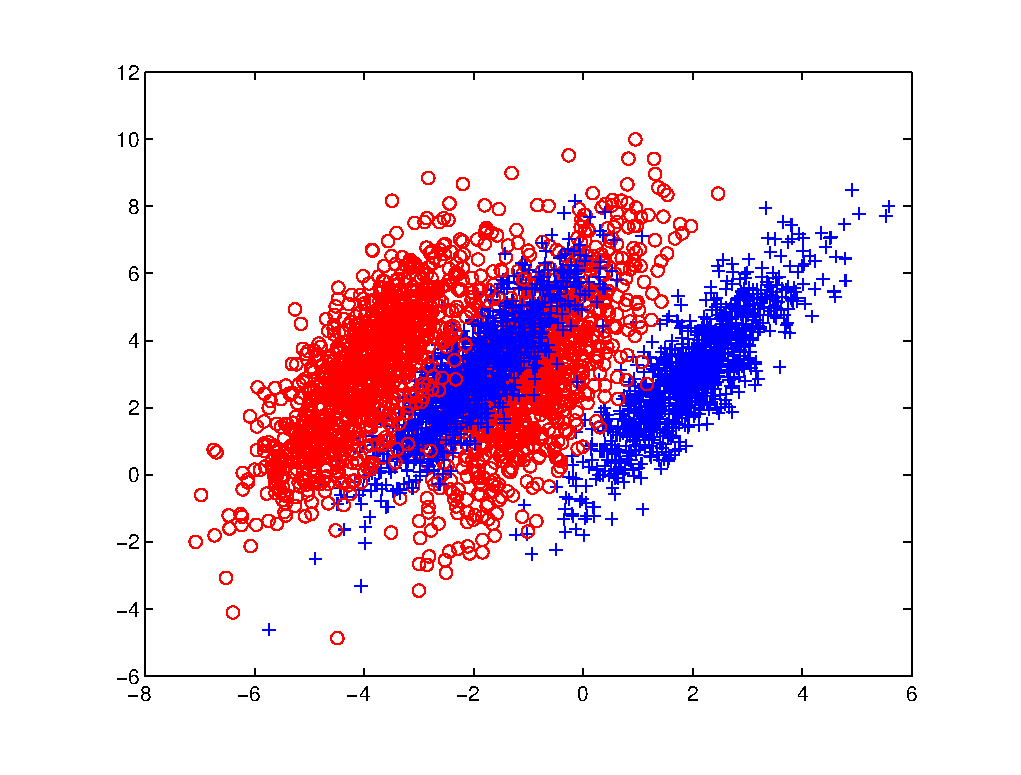
\includegraphics[width=2cm]{04_data_classification/08_classification/figures/pbt-simulation/pbt_tree_1.eps}}; 
%    \edge node[auto=right] {};
%    [.\node{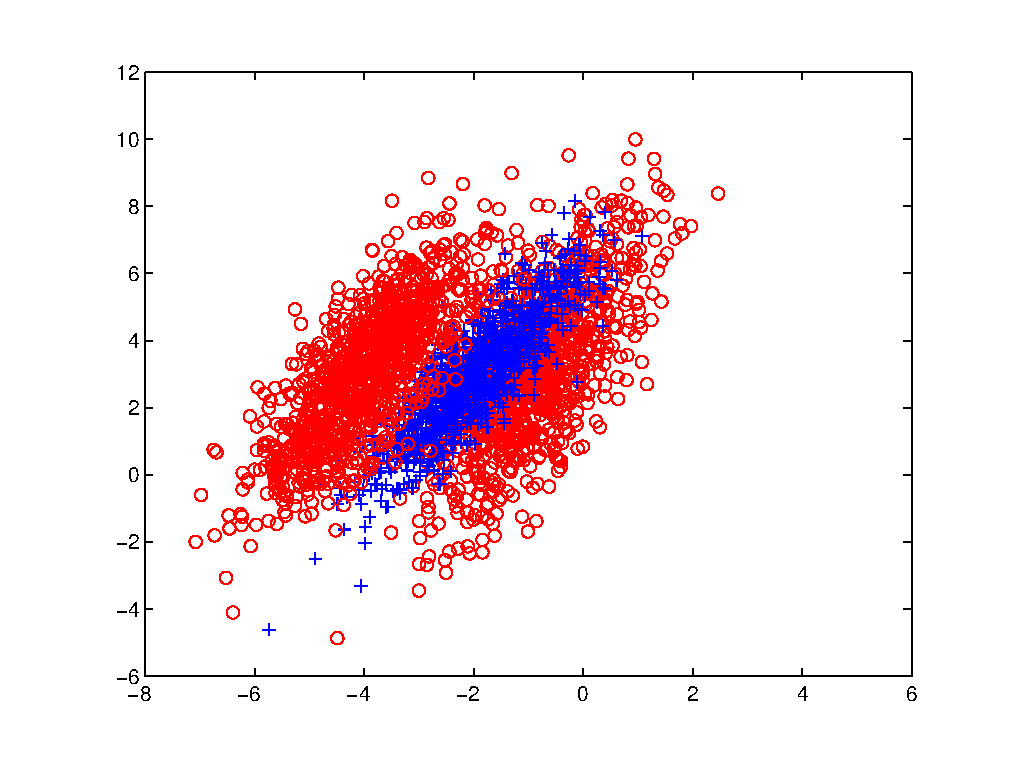
\includegraphics[width=2cm]{04_data_classification/08_classification/figures/pbt-simulation/pbt_tree_2_1.eps}};
%      \edge node[auto=right] {};  
%      [.\node{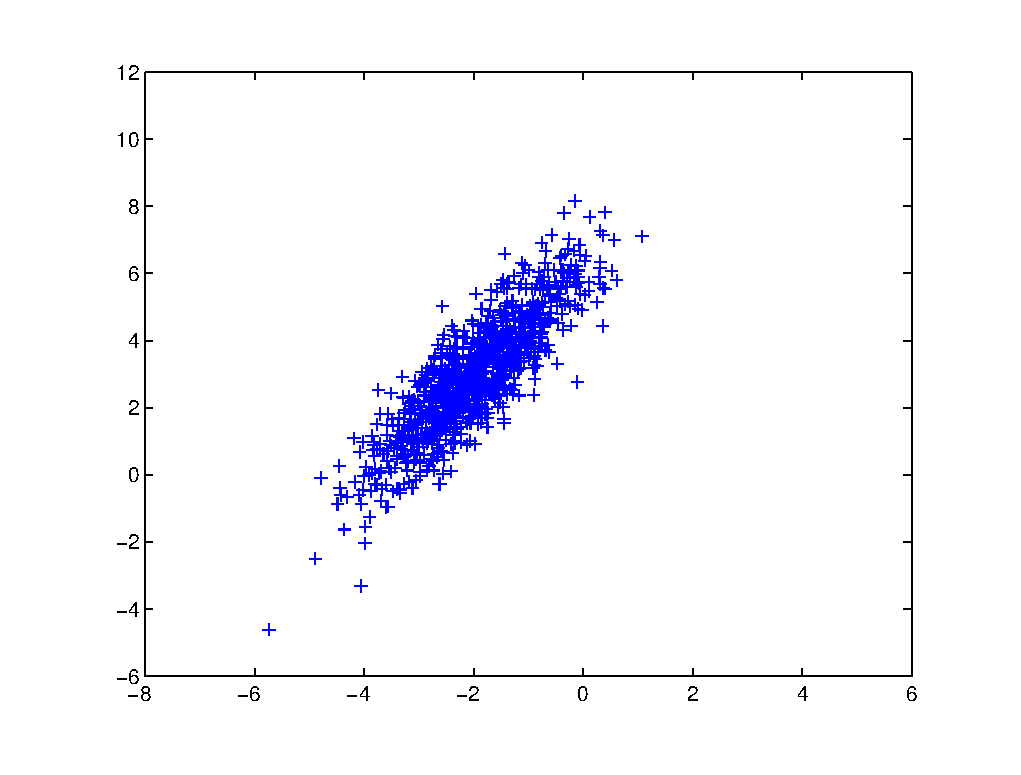
\includegraphics[width=2cm]{04_data_classification/08_classification/figures/pbt-simulation/pbt_tree_3_2.eps}}; ]
%      \edge node[auto=left] {};  
%      [.\node{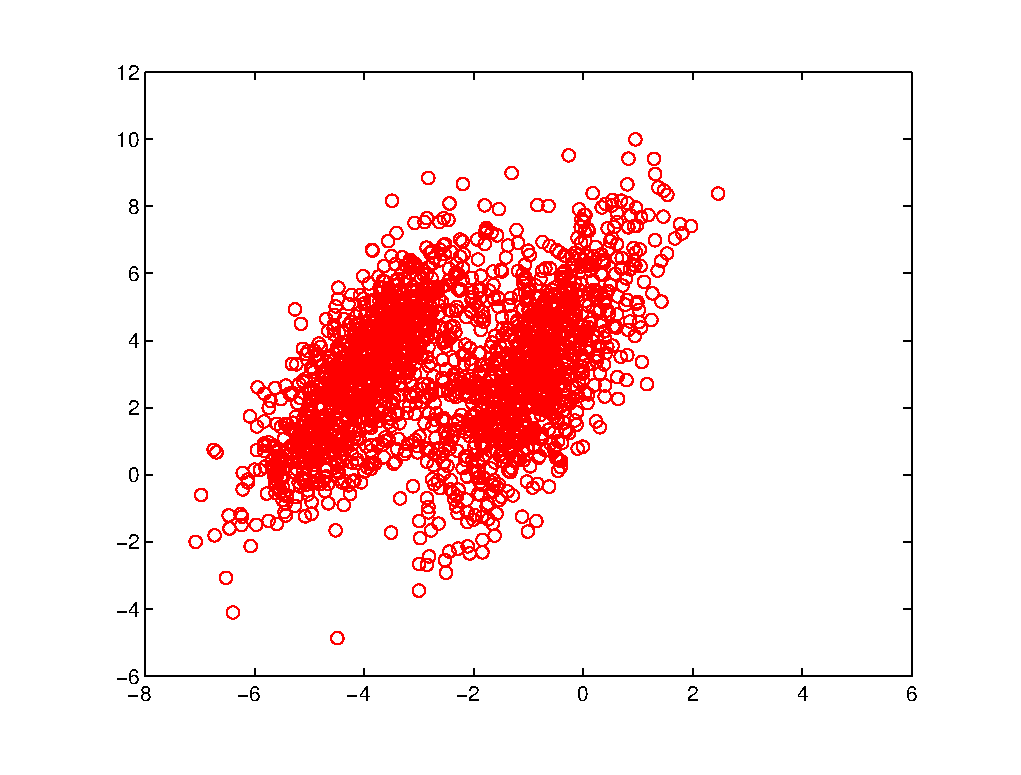
\includegraphics[width=2cm]{04_data_classification/08_classification/figures/pbt-simulation/pbt_tree_3_1.eps}}; ]
%    ]
%    \edge node[auto=left] {};
%    [.\node{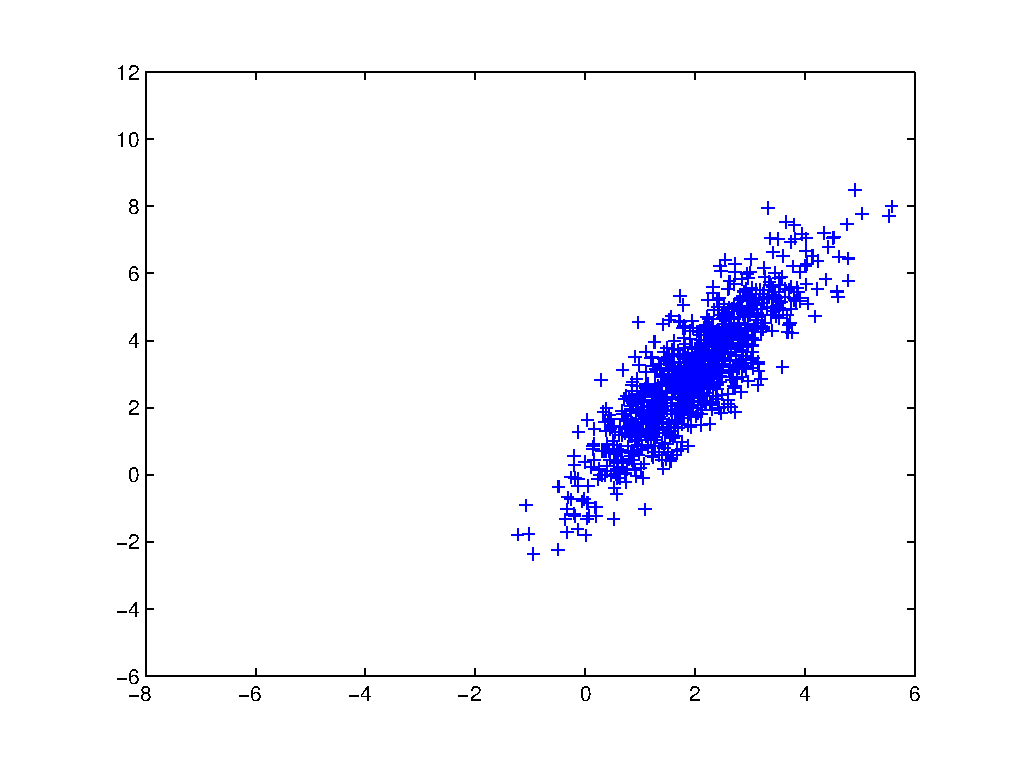
\includegraphics[width=2cm]{04_data_classification/08_classification/figures/pbt-simulation/pbt_tree_2_2.eps}};
%    ]
%    ];
%	\end{tikzpicture}
%\caption{Representation of the capabilities of the probabilistic boosting tree algorithm to split at each node of the tree the positive and negative samples.}
%\label{fig:pbtsim}
%\end{figure}

Probabilistic boosting-tree is another ensemble learning classifier which shares principles with AdaBoost but using them inside a decision tree (\cite{Tu2005}). % In the training stage, the probabilistic boosting-tree method grows a decision tree and at each node, a strong classifier is learnt in an almost comparable scheme to AdaBoost (see Eq. \ref{eq:strclaada}). Once the strong learner is trained, the training set will be split into two subsets which will be used to train the next strong classifiers in the next descending nodes. Thus, three cases are conceivable to decide which branch to propagate each sample training $\mathbf{x}_i$:
%\begin{itemize}
%	\item if $q(+1, \mathbf{x}_i) - \frac{1}{2} > \epsilon$ then $\mathbf{x}_i$ is propagated to the right branch set and a weight $w_i=1$ is assigned. 
%	\item if $q(-1, \mathbf{x}_i) - \frac{1}{2} > \epsilon$ then $\mathbf{x}_i$ is propagated to the left branch set and a weight $w_i=1$ is assigned.
%	\item else $\mathbf{x}_i$ will be propagated in both branches with $w_i=q(+1, \mathbf{x}_i)$ in the right branch and $w_i=q(-1, \mathbf{x}_i)$ in the left branch.
%\end{itemize}
%
%\noindent with $\mathbf{w} = w_i, i=\{1,\cdots,N\}$ corresponding to distribution of weights, $N$ the number of samples as in AdaBoost and $q(\cdot)$ is defined as:
%
%\begin{eqnarray}
%	q(+1, \mathbf{x}_i) & = & \frac{\exp(2H(\mathbf{x}_i))}{1+\exp(2H(\mathbf{x}_i))} \ , \label{eq:regada1} \\
%	q(-1, \mathbf{x}_i) & = & \frac{\exp(-2H(\mathbf{x}_i))}{1+\exp(-2H(\mathbf{x}_i))} \ . \label{eq:regada2}
%\end{eqnarray}
%
%Employing such a scheme tends to divide the data in such a way that positive and negative samples are naturally split as shown in Fig.~\ref{fig:pbtsim}.
%
%In the classification stage, the unlabelled sample $\mathbf{x}$ is propagated through the tree, where at each node, it will be classified by each strong classifier previously learned and where an estimation of the posterior distribution will be computed. The posterior distribution will correspond to the sum of the posterior distribution at each node of the decision tree.
\cite{Tiwari2009a,Tiwari2012,Tiwari2010,Viswanath2011} make use of the probabilistic boosting-tree classifier.

\item[$-$] \textbf{\textit{Kernel method:}}

A Gaussian process\footnote{Gaussian process implementation can be found at: \texttt{http://www.\allowbreak gaussianprocess.org/gpml/code/matlab/doc/index.html}} for classification is a kernel method in which it is assumed that the data can be represented by a single sample from a multivariate Gaussian distribution (\cite{Rasmussen2005}). % In the case of linear logistic regression for classification, the posterior probability can be expressed as:
%
%\begin{eqnarray}
%\centering
%	p(y_i|\mathbf{x}_i,\mathbf{w}) & = & \sigma(y_i f(\mathbf{x}_i)) \ , \label{eq:gp1} \\
%	f(\mathbf{x}_i) & = & \mathbf{x}_i^{\text{T}} \mathbf{w} \ , \nonumber
%\end{eqnarray}
%
%\noindent where $\sigma(\cdot)$ is the logistic function and $\mathbf{w}$ are the parameters vector of the model.
%
%Thus, the classification using Gaussian processes is based on assigning a Gaussian process prior over the function $f(\mathbf{x})$ which will be characterized by a mean function $\bar{f}$ and covariance function $K$. Thus, in the training stage, the best mean and covariance functions have to be inferred in regard to our training data using a Newton optimization and a Laplacian approximation.
%
%The prediction stage can be performed in two stages. First, for a new observation $\mathbf{x}_*$, the corresponding probability $p(f(\mathbf{x}_*)|f(\mathbf{x}))$ can be computed such that:
%\begin{eqnarray}
%	p(f(\mathbf{x}_*)|f(\mathbf{x})) & = & \mathcal{N}( K_*K^{-1}\bar{f}, K_{**}-K_*(K')^{-1}K_*^{\text{T}} ) \ , \nonumber \\
%	K' & = & K + W^{-1} \ , \label{eq:gp2} \\
%	W & = & \nabla \nabla \log p(\mathbf{y}|f(\mathbf{x})) \ , \nonumber
%\end{eqnarray}
%
%\noindent where $K_{**}$ is the variance of the testing sample $\mathbf{x}_*$, $K_{*}$ is the covariance of training-testing samples $\mathbf{x}$ and $\mathbf{x}_*$.
%
%Then, the function $f(\mathbf{x}_*)$ is squashed using the sigmoid function and the probability of the class membership can be defined such that:
%
%\begin{equation}
%	C(\mathbf{x}_*) = \sigma\left( \frac{\bar{f}(\mathbf{x_*})}{\sqrt{1+var(f(\mathbf{x}_*))}} \right) \ .
%	\label{eq:gp3}
%\end{equation}
Only the work of \cite{Kelm2007} used Gaussian process for classification in order to distinguish \ac{cap} in \ac{mrsi} data.

\item[$-$] \textbf{\textit{Sparse kernel methods:}}

In a classification scheme using Gaussian processes, when a prediction has to be performed, the whole training data will be used to assign a label to the new observations. That is why this method is also called kernel method. Sparse kernel category is composed of methods which rely only on a few labelled observations of the training set to assign the label of new observations (\cite{Bishop2006}).

\Acf{svm}\footnote{\ac{svm} implementation can be found at: \texttt{http://www.csie.ntu.edu.tw/\allowbreak $\sim$cjlin/libsvm/}} is a sparse kernel method aims at finding the best linear hyperplane (non-linear separation is discussed further) which separates two classes such that the margin between the two classes is maximized (\cite{Vapnik1963}).% The margin is in fact the region defined by two hyperplanes splitting the two classes, such that there are no points lying in between. The distance between these two hyperplanes is equal to $\frac{2}{\|\mathbf{w}\|}$ where $\mathbf{w}$ is the normal vector of the hyperplane splitting the classes. Thus, maximizing the margin is equivalent to minimizing the norm $\|\mathbf{w}\|$. Hence, This problem is solved by an optimization approach and formalized:
%
%\begin{equation}
%\begin{aligned}
%& \argmin_{\mathbf{w}}
%& & \frac{1}{2} \| \mathbf{w}^2\| \ , \\
%& \text{subject to}
%& & y_i(\mathbf{w}.\mathbf{x}_i - b) \geq 1, \; i = \{ 1, \ldots, N \} \ ,
%\end{aligned}
%\label{eq:svm1}
%\end{equation}
%
%\noindent where $\mathbf{x}_i$ is a training sample with is corresponding class label $y_i$.
%
%From Eq. \eqref{eq:svm1}, it is important to notice that only few points from the set of $N$ points have to be selected which will later define the hyperplane. This can be introduced in the optimization problem using Lagrange multipliers $\boldsymbol{\alpha}$. All points which are not lying on the margin will be assigned a corresponding $\alpha_i = 0$. This can be formalized as:
%
%\begin{equation}
%	\arg\min_{\mathbf{w},b } \max_{\boldsymbol{\alpha}\geq 0 } \left\{ \frac{1}{2}\|\mathbf{w}\|^2 - \sum_{i=1}^{n}{\alpha_i[y_i(\mathbf{w}\cdot \mathbf{x_i} - b)-1]} \right\} \ .
%	\label{eq:svm2}
%\end{equation}
%
%The different parameters can be inferred using quadratic programming. This version of \ac{svm} is known as hard-margin since no points can lie in the margin area. However, it is highly probable to not find any hyperplane splitting the classes such as specified previously. Thus, a soft-margin optimization approach was proposed (\cite{Cortes1995}), where points can lie on the margin but at the cost of a penalty $\xi_i$ which will be minimized in the optimization process such that:
%
%\begin{equation}
%\begin{aligned}
%\arg\min_{\mathbf{w},\mathbf{\xi}, b } \max_{\boldsymbol{\alpha},\boldsymbol{\beta} } & \left\{ \frac{1}{2}\|\mathbf{w}\|^2+C \sum_{i=1}^n \xi_i \right. \\
% & \left. - \sum_{i=1}^{n}{\alpha_i[y_i(\mathbf{w}\cdot \mathbf{x_i} - b) -1 + \xi_i]} - \sum_{i=1}^{n} \beta_i \xi_i \right\} \ .
%\end{aligned}
%\end{equation}
%
%The decision to assign the label to a new observation $\mathbf{x}_i$ is taken such that:
%
%\begin{equation}
%	C(\mathbf{x}_i) = \sign \left( \sum_{n=1}^{N} \alpha_n (\mathbf{x}_n . \mathbf{x}_i) + b_0 \right) \ ,
%	\label{eq:svmdec} 
%\end{equation}
%
%\noindent where $\mathbf{x}_n|n=\{1,\cdots,S\}$, $S$ being the support vectors.

\ac{svm} can also be used as a non-linear classifier by performing a kernel trick (\cite{Boser1992}). The original data $\mathbf{x}$ can be projected to a high-dimension space in which it is assumed that a linear hyperplane will split the classes. Different kernels are popular such as the \ac{rbf} kernel, polynomial kernels or Gaussian kernel.

In prostate \ac{cad} system, \ac{svm} is the most popular classification method and was used in a multitude of research works: \cite{Artan2009,Artan2010,Chan2003,Kelm2007,Litjens2011,Litjens2012,Liu2013,Lopes2011,Niaf2011,Niaf2012,Ozer2009,Ozer2010,Parfait2012,Peng2013,Sung2011,Tiwari2012,Vos2008,Vos2008a,Vos2010,Vos2012}.

\Acf{rvm} is a sparse version of Gaussian process previously presented and was proposed by \cite{Tipping2001}. \ac{rvm} is identical to a Gaussian process with the following covariance function (\cite{Quinonero-Candela2002}):

\begin{equation}
	K_{RVM}(\mathbf{x}_p,\mathbf{x}_q) = \sum_{j=1}^{M} \frac{1}{\alpha_j} \Phi_j ( \mathbf{x}_p ) \Phi_j ( \mathbf{x}_q ) \ ,
 	\label{eq:rvm}
\end{equation}

\noindent where $\phi(\cdot)$ is a Gaussian basis function, $\mathbf{x}_i|i=\{1,\cdots,N\}$ are the $N$ training points and $\boldsymbol{\alpha}$ are the weights vector.

As mentioned in \cite{Quinonero-Candela2002}, the sparsity regarding the relevance vector arises if $j \alpha_j^{-1} = 0$. The set of weights $\boldsymbol{\alpha}$ is inferred using the expectation maximization algorithm. \cite{Ozer2009,Ozer2010} make use of \ac{rvm} and make a comparison with \ac{svm} for the task of \ac{cap} detection.

\item[$-$] \textbf{\textit{Neural network:}} 
%
%\begin{figure}
%\centering
%\def\layersep{3cm}
%\begin{tikzpicture}[shorten >=1pt,draw=black!50, node distance=\layersep]
%    \tikzstyle{every pin edge}=[<-,shorten <=1pt]
%    \tikzstyle{neuron}=[circle,fill=black!25,minimum size=17pt,inner sep=0pt]
%    \tikzstyle{input neuron}=[neuron, fill=green!20];
%    \tikzstyle{output neuron}=[neuron, fill=red!80];
%    \tikzstyle{hidden neuron}=[neuron, fill=blue!40];
%    \tikzstyle{annot} = [text width=4em, text centered]
%
%    % Draw the input layer nodes
%    \foreach \name / \y in {1,...,3}
%    % This is the same as writing \foreach \name / \y in {1/1,2/2,3/3,4/4}
%        \node[input neuron] (I-\name) at (0,-\y) {\tiny $x_{ \y n }$};
%        
%   \node[input neuron] (I-4) at (0,-4.5) {\tiny $x_{in}$};
%   \draw[dashed,draw=black!50] (I-3) -- (I-4);
%
%    % Draw the hidden layer nodes
%    \foreach \name / \y in {1,...,4}
%        \path[yshift=0.5cm]
%            node[hidden neuron] (H-\name) at (\layersep,-\y cm) {\tiny $h_{ \y }\left(\sum \cdot \right)$};
%            
%    \node[hidden neuron] (H-5) at (\layersep,-5.5 cm) {\tiny $h_{j}\left(\sum \cdot \right)$};
%    \draw[dashed,draw=black!50] (H-4) -- (H-5);
%
%    % Draw the output layer node
%    	\node[output neuron,pin={[pin edge={->}]right:$C_{0}$}, right of=H-2] (O-1) {\tiny $\sigma\left(\sum \cdot \right)$};
%    	\node[output neuron,pin={[pin edge={->}]right:$C_{1}$}, right of=H-4] (O-2) {\tiny $\sigma\left(\sum \cdot \right)$};
%
%    % Connect every node in the input layer with every node in the
%    % hidden layer.
%    \foreach \source in {1,...,4}
%        \foreach \dest in {1,...,5}
%        		\draw[shorten >=1pt,->,draw=black!50] (I-\source)  -- (H-\dest);
%            %\path (I-\source) edge (H-\dest);
%    
%    % Draw the annotation for the weight for the first and last connections       
%    \draw[shorten >=1pt,->,draw=black!50] (I-1) -- (H-1) node [midway, above] (w111) {\scriptsize $w_{11}^{(1)}$};
%    \draw[shorten >=1pt,->,draw=black!50] (I-4) -- (H-5) node [midway, below] (w145) {\scriptsize $w_{ij}^{(1)}$};
%
%    % Connect every node in the hidden layer with the output layer
%    \foreach \source in {1,...,5}
%    		\foreach \dest in {1,...,2}
%        		\draw[shorten >=1pt,->,draw=black!50] (H-\source)  -- (O-\dest);
%        %\path (H-\source) edge (O);
%        
%    % Draw the annotation for the weight for the first and last connections       
%    \draw[shorten >=1pt,->,draw=black!50] (H-1) -- (O-1) node [midway, above] (w211) {\scriptsize $w_{11}^{(2)}$};
%    \draw[shorten >=1pt,->,draw=black!50] (H-5) -- (O-2) node [midway, below] (w251) {\scriptsize $w_{kj}^{(2)}$};
%
%    % Annotate the layers
%    \node[annot,above of=H-1, node distance=1cm] (hl) {\small Hidden layer};
%    \node[annot,left of=hl] {\small Input layer};
%    \node[annot,right of=hl] {\small Output layer};
%\end{tikzpicture}
%\caption{Representation of a neural network of the multilayer perceptron family.}
%\label{fig:mlp}
%\end{figure}

Multilayer perceptron is a feed-forward neural networks considered as the most successful model of this kind in pattern recognition (\cite{Bishop2006}). The most well known model used is based on a two layers. % where a prediction of an observation is computed as:
%
%\begin{equation}
%	C(\mathbf{x}_n,w_{ij}^{(1)},w_{kj}^{(2)}) = \sigma \left[ \sum_{j=0}^{M} w_{kj}^{(2)} \  h \left( \sum_{i=0}^{D} w_{ij}^{(1)} x_{in} \right) \right] \ ,
%	\label{eq:annmlp}
%\end{equation}
%
%\noindent where $h(\cdot)$ and $\sigma(\cdot)$ are two activation functions usually non-linear, $w_{ij}^{(1)}$ and $ w_{kj}^{(2)}$ are the weights associated with the linear combination with the input feature $\mathbf{x}_n$ and the hidden unit, respectively.
%A graphical representation of this network is presented in Fig.~\ref{fig:mlp}. Relating Fig.~\ref{fig:mlp} with Eq. \eqref{eq:annmlp}, it can be noted that this network is composed of some successive non-linear mapping of the input data. First, a linear combination of the input vector $\mathbf{x}_n$ is mapped into some hidden units through a set of weights $w_{ij}^{(1)}$. This combination becomes non-linear by the use of the activation function $h(\cdot)$ which is usually chosen to be a sigmoid function. Then, the output of the networks consists of a linear combination of the hidden units and the set of weights $w_{kj}^{(2)}$. This combination is also mapped non-linearly using an activation function $\sigma(\cdot)$ which is usually a logistic function. 
%Thus, the training of such a network resides in finding the best weights $w_{ij}^{(1)}$ and $ w_{kj}^{(2)}$ which will model the best our data. The error of this model can be computed as:
%
%\begin{equation}
%	E(w_{ij}^{(1)},w_{kj}^{(2)}) = \frac{1}{2} \sum_{n=1}^{N} \left( C(\mathbf{x}_n,w_{ij}^{(1)},w_{kj}^{(2)}) - y(\mathbf{x}_n) \right) ^{2} \ ,
%	\label{eq:mlpcost}
%\end{equation}
%
%\noindent where $\mathbf{x}_n|n=\{1,\cdots,N\}$ are the $N$ training vectors with their corresponding class label $y(\mathbf{x}_n)$.
%
%Thus the best set of weights can be inferred in an optimization framework where the error $E(\cdot)$ has to be minimized. This optimization can be performed using a gradient descent method where the derivative of Eq. \eqref{eq:mlpcost} can be computed using the backpropagation algorithm proposed by \cite{Rumelhart1988}. 
\cite{Matulewicz2013,Parfait2012} used this classifier to classify \ac{mrsi} spectra.

%\begin{equation}
%	\argmin_{w_{ij}^{(1)},w_{kj}^{(2)}} E(w_{ij}^{(1)},w_{kj}^{(2)}) \ . 
%	\label{eq:mlpopt}
%\end{equation}
%
%\begin{figure}
%\centering
%\def\layersep{3cm}
%\def\finallayersep{2.2cm}
%\begin{tikzpicture}[shorten >=1pt,draw=black!50, node distance=\layersep]
%    \tikzstyle{every pin edge}=[<-,shorten <=1pt]
%    \tikzstyle{neuron}=[circle,fill=black!25,minimum size=20pt,inner sep=0pt]
%    \tikzstyle{input neuron}=[neuron, fill=green!20];
%    \tikzstyle{output neuron}=[neuron, fill=red!80];
%    \tikzstyle{hidden neuron}=[neuron, fill=blue!20];
%    \tikzstyle{summation neuron}=[neuron, fill=blue!40];
%    \tikzstyle{annot} = [text width=4em, text centered]
%
%    % Draw the input layer nodes
%    \foreach \name / \y in {1,...,3}
%    % This is the same as writing \foreach \name / \y in {1/1,2/2,3/3,4/4}
%        \node[input neuron] (I-\name) at (0,-\y-1) {\tiny $x_{ \y n }$};
%        
%   \node[input neuron] (I-4) at (0,-5.5) {\tiny $x_{in}$};
%   \draw[dashed,draw=black!50] (I-3) -- (I-4);
%   
%   % Draw the pattern layer
%   \node[hidden neuron] (H-1) at (\layersep,0 cm) {\tiny $h_{11}\left(\sum \cdot \right)$};
%   \node[hidden neuron] (H-2) at (\layersep,-1 cm) {\tiny $h_{21}\left(\sum \cdot \right)$};
%   \node[hidden neuron] (H-3) at (\layersep,-2.5 cm) {\tiny $h_{31}\left(\sum \cdot \right)$};
%   \draw[dashed,draw=black!50] (H-2) -- (H-3);
%   
%   \begin{pgfonlayer}{background}
%	\path (H-1.west |- H-1.north)+(-0.2,0.2) node (a) {};
%    \path (H-3.east |- H-3.south)+(+0.2,-0.2) node (b) {};
%          
%    \path[fill=blue!10,rounded corners, draw=blue!50, dashed] (a) rectangle (b);
%   \end{pgfonlayer}
%   
%   \node[hidden neuron] (H-4) at (\layersep,-4.5 cm) {\tiny $h_{12}\left(\sum \cdot \right)$};
%   \node[hidden neuron] (H-5) at (\layersep,-5.5 cm) {\tiny $h_{22}\left(\sum \cdot \right)$};
%   \node[hidden neuron] (H-6) at (\layersep,-7 cm) {\tiny $h_{32}\left(\sum \cdot \right)$};
%   \draw[dashed,draw=black!50] (H-5) -- (H-6);
%   
%   \begin{pgfonlayer}{background}
%	\path (H-4.west |- H-4.north)+(-0.2,0.2) node (c) {};
%    \path (H-6.east |- H-6.south)+(+0.2,-0.2) node (d) {};
%          
%    \path[fill=blue!10,rounded corners, draw=blue!50, dashed] (c) rectangle (d);
%   \end{pgfonlayer}
%   
%   % Draw the summation layer
%   \begin{scope}[node distance=2cm]
%   \node[summation neuron, right of=H-2] (S-1) {\tiny $\sum_1 \cdot $};
%   \node[summation neuron, right of=H-5] (S-2) {\tiny $\sum_2 \cdot $};
%   \end{scope}
%   
%   % Draw the decision layer
%   \node[output neuron,pin={[pin edge={->}]right:$C$},] at (3*\finallayersep,-3.5 cm) (O) {$\sigma \left( \cdot \right)$};
%   
%   % Draw the networking from input layer to pattern layer
%   \foreach \source in {1,...,4}
%   		\foreach \dest in {1,...,6}
%   				\draw[shorten >=1pt,->,draw=black!50] (I-\source)  -- (H-\dest);
%   				
%   % Draw the networking from pattern layer to summation layer
%   \foreach \source in {1,...,3}
%   		\draw[shorten >=1pt,->,draw=black!50] (H-\source)  -- (S-1);
%   		
%   	\foreach \source in {4,...,6}
%   		\draw[shorten >=1pt,->,draw=black!50] (H-\source)  -- (S-2);
%   		
%   	% Draw from summation layer to ouput
%   	\draw[shorten >=1pt,->,draw=black!50] (S-1)  -- (O);
%   	\draw[shorten >=1pt,->,draw=black!50] (S-2)  -- (O);
%  
%    % Annotate the layers
%    \node[annot,above of=H-1, node distance=1cm] (hl) {\small Pattern layer};
%    \node[annot,left of=hl] {\small Input layer};
%    \begin{scope}[node distance=2cm]
%    \node[annot,right of=hl] {\small Summation layer};
%    \end{scope}
%    \node[annot,above of=O, node distance=4.5cm] (o) {\small Decision layer};
%\end{tikzpicture}
%\caption{Representation of a neural network of the probabilistic neural network family.}
%\label{fig:pnn}
%\end{figure}

Probabilistic neural networks are another type of feed-forward networks which can be derived from the multilayer perceptron case and was proposed by \cite{Specht1988}. This classifier can be modelled by changing the activation function of the hidden layer to an exponential function. % such that:
%
%\begin{equation}
%	h(\mathbf{x}_n) = \exp \left( - \frac{ (\mathbf{w}_j - \mathbf{x})^{\text{T}}(\mathbf{w}_j - \mathbf{x}) }{2\sigma^2} \right) \ ,
%	\label{eq:pnn1}
%\end{equation}
%
%\noindent where $\sigma$ is a free parameter set by the user.
%The other difference of the probabilistic neural networks when compared with the multilayer perceptron networks resides in the architecture as shown in Fig.~\ref{fig:pnn}. This network is formed by two hidden layers. The first hidden layer consists of the pattern layer, in which the mapping is done using Eq. \eqref{eq:pnn1}. This pattern layer is sub-divided into a number of groups corresponding to the number of classes. The second hidden layer corresponds to the summation layer which simply sums the output of each sub-group of the pattern layer. 
This method was used  by \cite{Ampeliotis2007,Ampeliotis2008,Viswanath2011} in order to perform the classification of their feature vector.

\item[$-$] \textbf{\textit{Graphical model classifiers:}}

Markov random fields can also be used as a lesion segmentation method to detect \ac{cap}. % First, we define $s$ as a pixel which will belong to a certain class denoted by $\omega_s$. The labelling process can be noted as $\omega = \{\omega_s, s \in I\}$ where $I$ is the set of all the pixels inside the image. The observations corresponding to \ac{si} in the image are noted $\mathcal{F} = \{ f_s | s \in I \}$. Thus, the image process $\mathcal{F}$ represents the deviation from the labelling process $\omega$ (\cite{Kato2001}). Hence, lesion segmentation is equivalent to estimating the best $\hat{\omega}$ which maximizes the posterior probability $p(\omega|\mathcal{F})$. Thus, using a Bayesian approach, this can be formulated such that:
%
%\begin{equation}
%	p(\omega|\mathcal{F}) = \argmax_{\omega} \prod_{s \in I} p(f_s | \omega_s) p(\omega) \ .
%	\label{eq:mrf1}
%\end{equation}
%
%It is generally assumed that $p(f_s | \omega_s)$ follows a Gaussian distribution and that the pixels classes $\lambda = \{1,2\}$ for a binary classification will be characterized by their respective mean $\mu_{\lambda}$ and standard deviation $\sigma_{\lambda}$. Then, $\omega$ is a Markov random field, thus:
%
%\begin{equation}
%	p(\omega) =  \frac{1}{Z} \exp\left( -U(\omega) \right)  \ ,
%	\label{eq:mrf2}
%\end{equation}
%
%\noindent where $Z$ is a normalization factor to obtain a probability value, $U(\cdot)$ is the energy function.
%
%Thus the segmentation problem can be solved as an optimization problem where the energy function $U(\cdot)$ has to be minimized. There are different possibilities to define the energy function $U(\cdot)$. However, it is common to define the energy function such that it combines two types of potential function: (i) a local term relative to the pixel itself and (ii) a smoothing prior which embeds neighbourhood information which will penalizes the energy function affecting the region homogeneity. This optimization of such a function can be performed using an algorithm such as iterated conditional modes (\cite{Kato2001}).
\cite{Liu2009,Ozer2010} used Markov random fields as an unsupervised method to segment lesions in multi-parametric \ac{mri} images.

\cite{Artan2009,Artan2010} used conditional random fields instead of Markov random fields to segment their \ac{mri} images. %The difference between these two methods resides in the fact that conditional probabilities are used instead of {\color{red}something here}.% such as:
%
%\begin{equation}
%	p(\omega|\mathcal{F}) =  \frac{1}{Z} \exp \left[ - \sum_{s \in I} V_{C1}(\omega_s|\mathcal{F}) - \sum_{\{s,r\} \in C } V_{C2} (\omega_s,\omega_r|\mathcal{F})  \right] \ .
%\label{eq:crf}
%\end{equation}
%
%\noindent $V_{C1}(\cdot)$ is the state (or partition) feature function and $V_{C2}(\cdot)$ is the transition (or edge) feature function (\cite{Kato2012}).

\end{enumerate}

\subsubsection{Model validation}

\begin{table}
	\caption{Overview of the model validation techniques used in \ac{cad} systems.}
	\small
	%\renewcommand{\arraystretch}{1.5}
	\begin{tabular}{p{.55\linewidth} p{.35\linewidth}}
		\hline \\ [-1.5ex]
		\textbf{Model validation techniques} & \textbf{References} \\ \\ [-1.5ex]
		\hline \\ [-1.5ex]
		\quad \acs{loo} & $[$1-8,11,18-22,24,25,33,37,39-41$]$ \\ \\ [-1.5ex]
		\quad \acs{kcv} & $[$10,23,29-33,38,36,42$]$ \\ \\ [-1.5ex]
		\hline
	\end{tabular}
	\label{tab:valmod}
\end{table}

In pattern recognition, the use of model validation techniques to assess the performance of trained classifiers is quite important. Two techniques are broadly used in the development of \ac{cad} system and are summarized in Tab. \ref{tab:valmod}.

The most popular technique used in \ac{cad} systems (see Tab. \ref{tab:valmod}) is the \acf{loo} technique. From the whole data, one patient is kept for validation and the other cases are used to train. This manipulation is repeated until each patient has been used for validation. This technique is popular when working with medical data due to the restricted number of patients included in datasets. Thus, it allows us to train on a fair number of patients even with a small dataset. However, this technique suffers from high variance and can be considered as an unreliable estimate (\cite{Efron1983}).

The other very well known technique used for assessing classifiers is the \acf{kcv} technique. This technique is based on splitting the dataset into $k$ subsets where the samples are randomly selected. Then, one fold is kept for the validation and the remaining subsets for training. The classification is then repeated as in the \ac{loo} technique. In our review, the typical values used for $k$ were set to three and five. This technique is more appropriate than the previous one since it does not suffer from large variance. However, the number of patients in the dataset needs to be large enough to apply such technique.

\subsubsection{Evaluation measure}\label{subsubsec:eval}

\begin{table}
	\caption{Overview of the evaluation metrics used in \ac{cad} systems.}
	\small
	%\renewcommand{\arraystretch}{1.5}
	\begin{tabular}{p{.55\linewidth} p{.35\linewidth}}
		\hline \\ [-1.5ex]
		\textbf{Evaluation metrics} & \textbf{References} \\ \\ [-1.5ex]
		\hline \\ [-1.5ex]
		\quad Accuracy & $[$4-5,13,26,32$]$ \\ \\ [-1.5ex]
		\quad Sensitivity - Specificity & $[$4-5,7,13,15,18,21-24,26,28-29,34-35$]$ \\ \\ [-1.5ex]
		\quad \acs{roc} - \acs{auc} & $[$2-3,6-9,14-20,24,30-33,36-41$]$ \\ \\ [-1.5ex]
		\quad \acs{froc} & $[$10-11,42$]$ \\ \\ [-1.5ex]
		\quad Dice's coefficient & $[$4-5,13,21$]$ \\ \\ [-1.5ex]
		\hline
	\end{tabular}
	\label{tab:evatec}
\end{table}

\begin{figure*}
\centering
\hspace*{\fill}
\subfigure[Comparison in terms of \ac{auc}-\ac{roc} of the methods using data from 1.5 Tesla \ac{mri} scanner.]{
\label{fig:auc15}
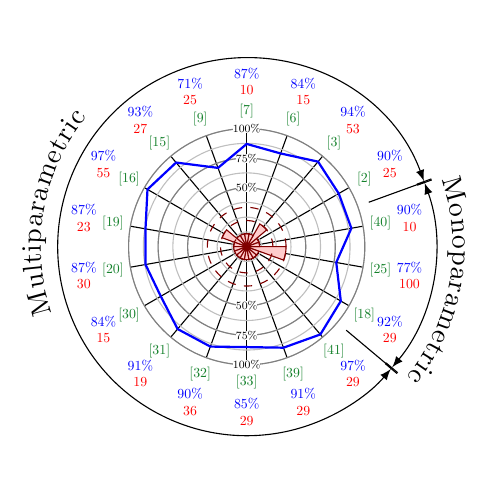
\begin{tikzpicture}[scale=.5,every node/.style={scale=0.5}]

\def\labels{
{\color{semiAuto}[2]},
{\color{semiAuto}[3]},
{\color{semiAuto}[6]},
{\color{semiAuto}[7]},
{\color{semiAuto}[9]},
{\color{semiAuto}[15]},
{\color{semiAuto}[16]},
{\color{semiAuto}[19]},
{\color{semiAuto}[20]},
{\color{semiAuto}[30]},
{\color{semiAuto}[31]},
{\color{semiAuto}[32]},
{\color{semiAuto}[33]},
{\color{semiAuto}[39]},
{\color{semiAuto}[41]},
{\color{semiAuto}[18]},
{\color{semiAuto}[25]},
{\color{semiAuto}[40]}
}

\def\reward{90,94,84,87,71,93,97,87,87,84,91,90,85,91,97,92,77,90}
\def\dbSize{25,53,15,10,25,27,55,23,30,15,19,36,29,29,29,29,100,10}
\def\dbClass{1,2,1,1,1,1,2,1,1,1,1,1,1,1,1,1,3,1}		
\def\cZoom{3} 
\def\percentageLabelAngle{90}
\def\nbeams{18}
\pgfmathsetmacro\beamAngle{(360/\nbeams)}
\pgfmathsetmacro\halfAngle{(180/\nbeams)}
%\def\globalRotation{10}
\pgfmathsetmacro\globalRotation{\halfAngle}

% draw manual AOV results
%\filldraw[blue!15!white,even odd rule] (0,0) circle [radius={\cZoom*.852}] (0,0) circle [radius={\cZoom*.8}];
%\draw[thin,color=blue!50!white,dashed] (0,0) circle [radius={\cZoom*.852}] (0,0) circle [radius={\cZoom*.8}];

%\foreach \x in {.125,.25, ...,1} { \draw[thin]  (0,0) circle [radius={2*\x}]; }
% draw the radiants
\foreach \n  [count=\ni] in \labels
{
\pgfmathsetmacro\cAngle{{(\ni*(360/\nbeams))+\globalRotation}}
\draw	(\cAngle:{\cZoom*1.15})  node[fill=white] {\n};
\draw [thin] (0,0) -- (\cAngle:{\cZoom*1}) ;

}

% draw the % rings 
\foreach \x in {12.5,25, ...,100} 
\draw [thin,color=gray!50] (0,0) circle [radius={\cZoom*\x/100}];

\foreach \x in {50,75,100}
{ 
     \draw [thin,color=black!50] (0,0) circle [radius={\cZoom/100*\x}];
     \foreach \a in {0, 180} \draw ({\percentageLabelAngle+\a}:{\cZoom*0.01*\x}) node  [inner sep=0pt,outer sep=0pt,fill=white,font=\fontsize{8}{8.5}\selectfont]{$\x\%$};
}

% draw the path of the percentages
\def\aux{{\reward}}
\pgfmathsetmacro\origin{\aux[\nbeams-1]} 
\draw [blue, thick] (\globalRotation:{\cZoom*\origin/100}) \foreach \n  [count=\ni] in \reward { -- ({(\ni*(360/\nbeams))+\globalRotation}:{\cZoom*\n/100}) } ;

% label all the percentags
\foreach \n [count=\ni] in \dbSize 
{
	\pgfmathsetmacro\cAngle{{(\ni*(360/\nbeams))+\globalRotation}}
	\pgfmathsetmacro\nreward{\aux[\ni-1]}
	\draw (\cAngle:{\cZoom*1.4}) node[align=center] {{\color{blue}\nreward $\%$} \\ {\color{red}\n} };
} ;

% draw the database rose
\def\dbScale{\9}
\foreach \n [count=\ni] in \dbClass
\filldraw[fill=red!20!white, draw=red!50!black]
(0,0) -- ({\ni*(360/\nbeams)-\halfAngle+\globalRotation}:{\cZoom*\n/9}) arc ({\ni*(360/\nbeams)-\halfAngle+\globalRotation}:{\ni*(360/\nbeams)+\halfAngle+\globalRotation}:{\cZoom*\n/9}) -- cycle;
\foreach \x in {1,2,3}
\draw [thin,color=red!50!black,dashed] (0,0) circle [radius={\cZoom*\x/9}];

%% draw the domain of each class 
  \def\puta{	15/0/{Multiparametric},
  			3/15/{Monoparametric}}
%\def\putaa{  	2/9/{Other+ML},
%  			3/11/{ML},
%  			2/14/{ML+ACM}}

\foreach \numElm/\contadorQueNoSeCalcular/\name [count=\ni] in \puta
 {

 	\pgfmathsetmacro\initialAngle{(\contadorQueNoSeCalcular*\beamAngle)+\halfAngle+\globalRotation}
 	\pgfmathsetmacro\finalAngle  {((\numElm+\contadorQueNoSeCalcular)*\beamAngle)+\halfAngle+\globalRotation}
	\pgfmathsetmacro\l  {\cZoom*1.5+.3pt}
	\draw (\initialAngle:{\cZoom*1.6}) -- (\initialAngle:{\cZoom*1.1});
	\draw [ |<->|,>=latex] (\initialAngle:\l) arc (\initialAngle:\finalAngle:\l) ;    									 
	\pgfmathsetmacro\r  {\cZoom*1.5+.45pt}
    	{\draw [decoration={raise=4pt,text along path,text={\name},text align={center}},decorate] (\finalAngle:\r) arc (\finalAngle:\initialAngle:\r);}
  }
%  
%   \foreach \numElm/\contadorQueNoSeCalcular/\name [count=\ni] in \putaa
% {
%
% 	\pgfmathsetmacro\initialAngle{(\contadorQueNoSeCalcular*\beamAngle)+\halfAngle+\globalRotation}
% 	\pgfmathsetmacro\finalAngle  {((\numElm+\contadorQueNoSeCalcular)*\beamAngle)+\halfAngle+\globalRotation}
%	\pgfmathsetmacro\l  {\cZoom*1.5+.3pt}
%	\draw (\initialAngle:{\cZoom*1.6}) -- (\initialAngle:{\cZoom*1.1});
%	\draw [ |<->|,>=latex] (\initialAngle:\l) arc (\initialAngle:\finalAngle:\l) ;    									 
%	\pgfmathsetmacro\r  {\cZoom*1.5+.7pt}
%    	{\draw [decoration={text along path, text={\name},text align={center}},decorate] (\initialAngle:\r) arc (\initialAngle:\finalAngle:\r);}    			 
%  }
        
\end{tikzpicture}}\hfill
\subfigure[Comparison in terms of \ac{auc}-\ac{roc} of the methods using data from 3.0 Tesla \ac{mri} scanner.]{
\label{fig:auc30}
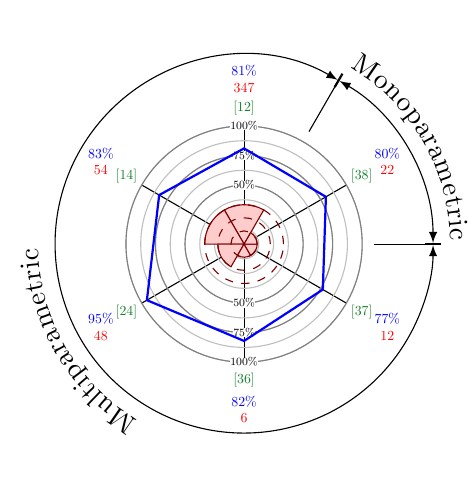
\begin{tikzpicture}[scale=.5,every node/.style={scale=0.5}]

\def\labels{
{\color{semiAuto}[12]},
{\color{semiAuto}[14]},
{\color{semiAuto}[24]},
{\color{semiAuto}[36]},
{\color{semiAuto}[37]},
{\color{semiAuto}[38]}
}

\def\reward{81,83,95,82,77,80}
\def\dbSize{347,54,48,6,12,22}
\def\dbClass{3,3,2,1,1,1}		
\def\cZoom{3} 
\def\percentageLabelAngle{90}
\def\nbeams{6}
\pgfmathsetmacro\beamAngle{(360/\nbeams)}
\pgfmathsetmacro\halfAngle{(180/\nbeams)}
%\def\globalRotation{10}
\pgfmathsetmacro\globalRotation{\halfAngle}

% draw manual AOV results
%\filldraw[blue!15!white,even odd rule] (0,0) circle [radius={\cZoom*.852}] (0,0) circle [radius={\cZoom*.8}];
%\draw[thin,color=blue!50!white,dashed] (0,0) circle [radius={\cZoom*.852}] (0,0) circle [radius={\cZoom*.8}];

%\foreach \x in {.125,.25, ...,1} { \draw[thin]  (0,0) circle [radius={2*\x}]; }
% draw the radiants
\foreach \n  [count=\ni] in \labels
{
\pgfmathsetmacro\cAngle{{(\ni*(360/\nbeams))+\globalRotation}}
\draw	(\cAngle:{\cZoom*1.15})  node[fill=white] {\n};
\draw [thin] (0,0) -- (\cAngle:{\cZoom*1}) ;

}

% draw the % rings 
\foreach \x in {12.5,25, ...,100} 
\draw [thin,color=gray!50] (0,0) circle [radius={\cZoom*\x/100}];

\foreach \x in {50,75,100}
{ 
     \draw [thin,color=black!50] (0,0) circle [radius={\cZoom/100*\x}];
     \foreach \a in {0, 180} \draw ({\percentageLabelAngle+\a}:{\cZoom*0.01*\x}) node  [inner sep=0pt,outer sep=0pt,fill=white,font=\fontsize{8}{8.5}\selectfont]{$\x\%$};
}

% draw the path of the percentages
\def\aux{{\reward}}
\pgfmathsetmacro\origin{\aux[\nbeams-1]} 
\draw [blue, thick] (\globalRotation:{\cZoom*\origin/100}) \foreach \n  [count=\ni] in \reward { -- ({(\ni*(360/\nbeams))+\globalRotation}:{\cZoom*\n/100}) } ;

% label all the percentags
\foreach \n [count=\ni] in \dbSize 
{
	\pgfmathsetmacro\cAngle{{(\ni*(360/\nbeams))+\globalRotation}}
	\pgfmathsetmacro\nreward{\aux[\ni-1]}
	\draw (\cAngle:{\cZoom*1.4}) node[align=center] {{\color{blue}\nreward $\%$} \\ {\color{red}\n} };
} ;

% draw the database rose
\def\dbScale{\9}
\foreach \n [count=\ni] in \dbClass
\filldraw[fill=red!20!white, draw=red!50!black]
(0,0) -- ({\ni*(360/\nbeams)-\halfAngle+\globalRotation}:{\cZoom*\n/9}) arc ({\ni*(360/\nbeams)-\halfAngle+\globalRotation}:{\ni*(360/\nbeams)+\halfAngle+\globalRotation}:{\cZoom*\n/9}) -- cycle;
\foreach \x in {1,2,3}
\draw [thin,color=red!50!black,dashed] (0,0) circle [radius={\cZoom*\x/9}];

%% draw the domain of each class 
  \def\puta{	5/0/{Multiparametric},
  			1/5/{Monoparametric}}
%\def\putaa{  	2/9/{Other+ML},
%  			3/11/{ML},
%  			2/14/{ML+ACM}}

\foreach \numElm/\contadorQueNoSeCalcular/\name [count=\ni] in \puta
 {

 	\pgfmathsetmacro\initialAngle{(\contadorQueNoSeCalcular*\beamAngle)+\halfAngle+\globalRotation}
 	\pgfmathsetmacro\finalAngle  {((\numElm+\contadorQueNoSeCalcular)*\beamAngle)+\halfAngle+\globalRotation}
	\pgfmathsetmacro\l  {\cZoom*1.5+.3pt}
	\draw (\initialAngle:{\cZoom*1.6}) -- (\initialAngle:{\cZoom*1.1});
	\draw [ |<->|,>=latex] (\initialAngle:\l) arc (\initialAngle:\finalAngle:\l) ;    									 
	\pgfmathsetmacro\r  {\cZoom*1.5+.45pt}
    	{\draw [decoration={raise=4pt,text along path,  text={\name},text align={center}},decorate] (\finalAngle:\r) arc (\finalAngle:\initialAngle:\r);}
  }
%  
%   \foreach \numElm/\contadorQueNoSeCalcular/\name [count=\ni] in \putaa
% {
%
% 	\pgfmathsetmacro\initialAngle{(\contadorQueNoSeCalcular*\beamAngle)+\halfAngle+\globalRotation}
% 	\pgfmathsetmacro\finalAngle  {((\numElm+\contadorQueNoSeCalcular)*\beamAngle)+\halfAngle+\globalRotation}
%	\pgfmathsetmacro\l  {\cZoom*1.5+.3pt}
%	\draw (\initialAngle:{\cZoom*1.6}) -- (\initialAngle:{\cZoom*1.1});
%	\draw [ |<->|,>=latex] (\initialAngle:\l) arc (\initialAngle:\finalAngle:\l) ;    									 
%	\pgfmathsetmacro\r  {\cZoom*1.5+.7pt}
%    	{\draw [decoration={text along path, text={\name},text align={center}},decorate] (\initialAngle:\r) arc (\initialAngle:\finalAngle:\r);}    			 
%  }
        
\end{tikzpicture}
}
\hspace*{\fill}
\caption{Comparison of the results in terms of AUC for 1.5 and 3.0 Tesla \ac{mri} scanners. The {\color{blue}blue} value represents the metric and are graphically reported in the blue curve in the center of the figure. The {\color{red}red} value and areas correspond to the number of patients in the dataset. The numbers between brackets in {\color{semiAuto}green} correspond to the reference as reported in Tab. \ref{tab:sumpap}.}
\label{fig:auc}
\end{figure*}

%------------------------------------------------------------------------------------------------------------------------

\begin{figure*}%
\centering
\hspace*{\fill}
\subfigure[Comparison in terms of sensitivity of the methods using data from 1.5 Tesla \ac{mri} scanner.]{
\label{fig:sens15}
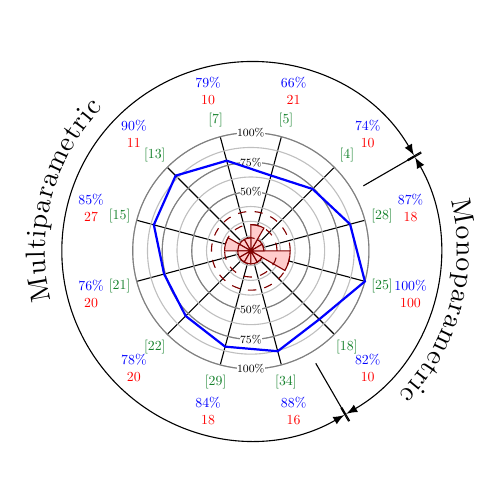
\begin{tikzpicture}[scale=.5,every node/.style={scale=0.5}]

\def\labels{
{\color{semiAuto}[4]},
{\color{semiAuto}[5]},
{\color{semiAuto}[7]},
{\color{semiAuto}[13]},
{\color{semiAuto}[15]},
{\color{semiAuto}[21]},
{\color{semiAuto}[22]},
{\color{semiAuto}[29]},
{\color{semiAuto}[34]},
{\color{semiAuto}[18]},
{\color{semiAuto}[25]},
{\color{semiAuto}[28]}
}

\def\reward{74,66,79,90,85,76,78,84,88,82,100,87}
\def\dbSize{10,21,10,11,27,20,20,18,16,10,100,18}
\def\dbClass{1,2,1,1,2,1,1,1,1,1,3,1}		
\def\cZoom{3} 
\def\percentageLabelAngle{90}
\def\nbeams{12}
\pgfmathsetmacro\beamAngle{(360/\nbeams)}
\pgfmathsetmacro\halfAngle{(180/\nbeams)}
%\def\globalRotation{10}
\pgfmathsetmacro\globalRotation{\halfAngle}

% draw manual AOV results
%\filldraw[blue!15!white,even odd rule] (0,0) circle [radius={\cZoom*.852}] (0,0) circle [radius={\cZoom*.8}];
%\draw[thin,color=blue!50!white,dashed] (0,0) circle [radius={\cZoom*.852}] (0,0) circle [radius={\cZoom*.8}];

%\foreach \x in {.125,.25, ...,1} { \draw[thin]  (0,0) circle [radius={2*\x}]; }
% draw the radiants
\foreach \n  [count=\ni] in \labels
{
\pgfmathsetmacro\cAngle{{(\ni*(360/\nbeams))+\globalRotation}}
\draw	(\cAngle:{\cZoom*1.15})  node[fill=white] {\n};
\draw [thin] (0,0) -- (\cAngle:{\cZoom*1}) ;

}

% draw the % rings 
\foreach \x in {12.5,25, ...,100} 
\draw [thin,color=gray!50] (0,0) circle [radius={\cZoom*\x/100}];

\foreach \x in {50,75,100}
{ 
     \draw [thin,color=black!50] (0,0) circle [radius={\cZoom/100*\x}];
     \foreach \a in {0, 180} \draw ({\percentageLabelAngle+\a}:{\cZoom*0.01*\x}) node  [inner sep=0pt,outer sep=0pt,fill=white,font=\fontsize{8}{8.5}\selectfont]{$\x\%$};
}

% draw the path of the percentages
\def\aux{{\reward}}
\pgfmathsetmacro\origin{\aux[\nbeams-1]} 
\draw [blue, thick] (\globalRotation:{\cZoom*\origin/100}) \foreach \n  [count=\ni] in \reward { -- ({(\ni*(360/\nbeams))+\globalRotation}:{\cZoom*\n/100}) } ;

% label all the percentags
\foreach \n [count=\ni] in \dbSize 
{
	\pgfmathsetmacro\cAngle{{(\ni*(360/\nbeams))+\globalRotation}}
	\pgfmathsetmacro\nreward{\aux[\ni-1]}
	\draw (\cAngle:{\cZoom*1.4}) node[align=center] {{\color{blue}\nreward $\%$} \\ {\color{red}\n} };
} ;

% draw the database rose
\def\dbScale{\9}
\foreach \n [count=\ni] in \dbClass
\filldraw[fill=red!20!white, draw=red!50!black]
(0,0) -- ({\ni*(360/\nbeams)-\halfAngle+\globalRotation}:{\cZoom*\n/9}) arc ({\ni*(360/\nbeams)-\halfAngle+\globalRotation}:{\ni*(360/\nbeams)+\halfAngle+\globalRotation}:{\cZoom*\n/9}) -- cycle;
\foreach \x in {1,2,3}
\draw [thin,color=red!50!black,dashed] (0,0) circle [radius={\cZoom*\x/9}];

%% draw the domain of each class 
  \def\puta{	9/0/{Multiparametric},
  			3/9/{Monoparametric}}
%\def\putaa{  	2/9/{Other+ML},
%  			3/11/{ML},
%  			2/14/{ML+ACM}}

\foreach \numElm/\contadorQueNoSeCalcular/\name [count=\ni] in \puta
 {

 	\pgfmathsetmacro\initialAngle{(\contadorQueNoSeCalcular*\beamAngle)+\halfAngle+\globalRotation}
 	\pgfmathsetmacro\finalAngle  {((\numElm+\contadorQueNoSeCalcular)*\beamAngle)+\halfAngle+\globalRotation}
	\pgfmathsetmacro\l  {\cZoom*1.5+.3pt}
	\draw (\initialAngle:{\cZoom*1.6}) -- (\initialAngle:{\cZoom*1.1});
	\draw [ |<->|,>=latex] (\initialAngle:\l) arc (\initialAngle:\finalAngle:\l) ;    									 
	\pgfmathsetmacro\r  {\cZoom*1.5+.45pt}
    	{\draw [decoration={raise=4pt,text along path,  text={\name},text align={center}},decorate] (\finalAngle:\r) arc (\finalAngle:\initialAngle:\r);}
  }
%  
%   \foreach \numElm/\contadorQueNoSeCalcular/\name [count=\ni] in \putaa
% {
%
% 	\pgfmathsetmacro\initialAngle{(\contadorQueNoSeCalcular*\beamAngle)+\halfAngle+\globalRotation}
% 	\pgfmathsetmacro\finalAngle  {((\numElm+\contadorQueNoSeCalcular)*\beamAngle)+\halfAngle+\globalRotation}
%	\pgfmathsetmacro\l  {\cZoom*1.5+.3pt}
%	\draw (\initialAngle:{\cZoom*1.6}) -- (\initialAngle:{\cZoom*1.1});
%	\draw [ |<->|,>=latex] (\initialAngle:\l) arc (\initialAngle:\finalAngle:\l) ;    									 
%	\pgfmathsetmacro\r  {\cZoom*1.5+.7pt}
%    	{\draw [decoration={text along path, text={\name},text align={center}},decorate] (\initialAngle:\r) arc (\initialAngle:\finalAngle:\r);}    			 
%  }
        
\end{tikzpicture}}\hfill
\subfigure[Comparison in terms of specificity of the methods using data from 1.5 Tesla \ac{mri} scanner.]{
\label{fig:spec15}
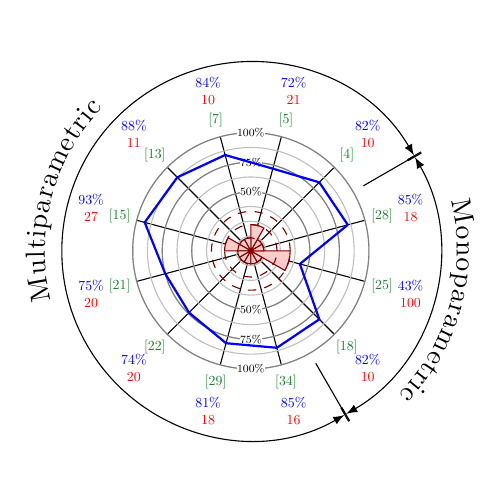
\begin{tikzpicture}[scale=.5,every node/.style={scale=0.5}]

\def\labels{
{\color{semiAuto}[4]},
{\color{semiAuto}[5]},
{\color{semiAuto}[7]},
{\color{semiAuto}[13]},
{\color{semiAuto}[15]},
{\color{semiAuto}[21]},
{\color{semiAuto}[22]},
{\color{semiAuto}[29]},
{\color{semiAuto}[34]},
{\color{semiAuto}[18]},
{\color{semiAuto}[25]},
{\color{semiAuto}[28]}
}

\def\reward{82,72,84,88,93,75,74,81,85,82,43,85}
\def\dbSize{10,21,10,11,27,20,20,18,16,10,100,18}
\def\dbClass{1,2,1,1,2,1,1,1,1,1,3,1}		
\def\cZoom{3} 
\def\percentageLabelAngle{90}
\def\nbeams{12}
\pgfmathsetmacro\beamAngle{(360/\nbeams)}
\pgfmathsetmacro\halfAngle{(180/\nbeams)}
%\def\globalRotation{10}
\pgfmathsetmacro\globalRotation{\halfAngle}

% draw manual AOV results
%\filldraw[blue!15!white,even odd rule] (0,0) circle [radius={\cZoom*.852}] (0,0) circle [radius={\cZoom*.8}];
%\draw[thin,color=blue!50!white,dashed] (0,0) circle [radius={\cZoom*.852}] (0,0) circle [radius={\cZoom*.8}];

%\foreach \x in {.125,.25, ...,1} { \draw[thin]  (0,0) circle [radius={2*\x}]; }
% draw the radiants
\foreach \n  [count=\ni] in \labels
{
\pgfmathsetmacro\cAngle{{(\ni*(360/\nbeams))+\globalRotation}}
\draw	(\cAngle:{\cZoom*1.15})  node[fill=white] {\n};
\draw [thin] (0,0) -- (\cAngle:{\cZoom*1}) ;

}

% draw the % rings 
\foreach \x in {12.5,25, ...,100} 
\draw [thin,color=gray!50] (0,0) circle [radius={\cZoom*\x/100}];

\foreach \x in {50,75,100}
{ 
     \draw [thin,color=black!50] (0,0) circle [radius={\cZoom/100*\x}];
     \foreach \a in {0, 180} \draw ({\percentageLabelAngle+\a}:{\cZoom*0.01*\x}) node  [inner sep=0pt,outer sep=0pt,fill=white,font=\fontsize{8}{8.5}\selectfont]{$\x\%$};
}

% draw the path of the percentages
\def\aux{{\reward}}
\pgfmathsetmacro\origin{\aux[\nbeams-1]} 
\draw [blue, thick] (\globalRotation:{\cZoom*\origin/100}) \foreach \n  [count=\ni] in \reward { -- ({(\ni*(360/\nbeams))+\globalRotation}:{\cZoom*\n/100}) } ;

% label all the percentags
\foreach \n [count=\ni] in \dbSize 
{
	\pgfmathsetmacro\cAngle{{(\ni*(360/\nbeams))+\globalRotation}}
	\pgfmathsetmacro\nreward{\aux[\ni-1]}
	\draw (\cAngle:{\cZoom*1.4}) node[align=center] {{\color{blue}\nreward $\%$} \\ {\color{red}\n} };
} ;

% draw the database rose
\def\dbScale{\9}
\foreach \n [count=\ni] in \dbClass
\filldraw[fill=red!20!white, draw=red!50!black]
(0,0) -- ({\ni*(360/\nbeams)-\halfAngle+\globalRotation}:{\cZoom*\n/9}) arc ({\ni*(360/\nbeams)-\halfAngle+\globalRotation}:{\ni*(360/\nbeams)+\halfAngle+\globalRotation}:{\cZoom*\n/9}) -- cycle;
\foreach \x in {1,2,3}
\draw [thin,color=red!50!black,dashed] (0,0) circle [radius={\cZoom*\x/9}];

%% draw the domain of each class 
  \def\puta{	9/0/{Multiparametric},
  			3/9/{Monoparametric}}
%\def\putaa{  	2/9/{Other+ML},
%  			3/11/{ML},
%  			2/14/{ML+ACM}}

\foreach \numElm/\contadorQueNoSeCalcular/\name [count=\ni] in \puta
 {

 	\pgfmathsetmacro\initialAngle{(\contadorQueNoSeCalcular*\beamAngle)+\halfAngle+\globalRotation}
 	\pgfmathsetmacro\finalAngle  {((\numElm+\contadorQueNoSeCalcular)*\beamAngle)+\halfAngle+\globalRotation}
	\pgfmathsetmacro\l  {\cZoom*1.5+.3pt}
	\draw (\initialAngle:{\cZoom*1.6}) -- (\initialAngle:{\cZoom*1.1});
	\draw [ |<->|,>=latex] (\initialAngle:\l) arc (\initialAngle:\finalAngle:\l) ;    									 
	\pgfmathsetmacro\r  {\cZoom*1.5+.45pt}
    	{\draw [decoration={raise=4pt,text along path,  text={\name},text align={center}},decorate] (\finalAngle:\r) arc (\finalAngle:\initialAngle:\r);}
  }
%  
%   \foreach \numElm/\contadorQueNoSeCalcular/\name [count=\ni] in \putaa
% {
%
% 	\pgfmathsetmacro\initialAngle{(\contadorQueNoSeCalcular*\beamAngle)+\halfAngle+\globalRotation}
% 	\pgfmathsetmacro\finalAngle  {((\numElm+\contadorQueNoSeCalcular)*\beamAngle)+\halfAngle+\globalRotation}
%	\pgfmathsetmacro\l  {\cZoom*1.5+.3pt}
%	\draw (\initialAngle:{\cZoom*1.6}) -- (\initialAngle:{\cZoom*1.1});
%	\draw [ |<->|,>=latex] (\initialAngle:\l) arc (\initialAngle:\finalAngle:\l) ;    									 
%	\pgfmathsetmacro\r  {\cZoom*1.5+.7pt}
%    	{\draw [decoration={text along path, text={\name},text align={center}},decorate] (\initialAngle:\r) arc (\initialAngle:\finalAngle:\r);}    			 
%  }
        
\end{tikzpicture}
}
\hspace*{\fill}
\\
\hspace*{\fill}
\subfigure[Comparison in terms of sensitivity of the methods using data from 3.0 Tesla \ac{mri} scanner.]{
\label{fig:sens30}
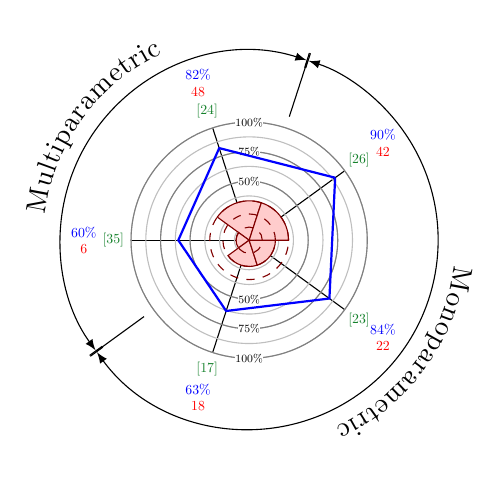
\begin{tikzpicture}[scale=.5,every node/.style={scale=0.5}]

\def\labels{
{\color{semiAuto}[24]},
{\color{semiAuto}[35]},
{\color{semiAuto}[17]},
{\color{semiAuto}[23]},
{\color{semiAuto}[26]}
}

\def\reward{82,60,63,84,90}
\def\dbSize{48,6,18,22,42}
\def\dbClass{3,1,2,2,3}		
\def\cZoom{3} 
\def\percentageLabelAngle{90}
\def\nbeams{5}
\pgfmathsetmacro\beamAngle{(360/\nbeams)}
\pgfmathsetmacro\halfAngle{(180/\nbeams)}
%\def\globalRotation{10}
\pgfmathsetmacro\globalRotation{\halfAngle}

% draw manual AOV results
%\filldraw[blue!15!white,even odd rule] (0,0) circle [radius={\cZoom*.852}] (0,0) circle [radius={\cZoom*.8}];
%\draw[thin,color=blue!50!white,dashed] (0,0) circle [radius={\cZoom*.852}] (0,0) circle [radius={\cZoom*.8}];

%\foreach \x in {.125,.25, ...,1} { \draw[thin]  (0,0) circle [radius={2*\x}]; }
% draw the radiants
\foreach \n  [count=\ni] in \labels
{
\pgfmathsetmacro\cAngle{{(\ni*(360/\nbeams))+\globalRotation}}
\draw	(\cAngle:{\cZoom*1.15})  node[fill=white] {\n};
\draw [thin] (0,0) -- (\cAngle:{\cZoom*1}) ;

}

% draw the % rings 
\foreach \x in {12.5,25, ...,100} 
\draw [thin,color=gray!50] (0,0) circle [radius={\cZoom*\x/100}];

\foreach \x in {50,75,100}
{ 
     \draw [thin,color=black!50] (0,0) circle [radius={\cZoom/100*\x}];
     \foreach \a in {0, 180} \draw ({\percentageLabelAngle+\a}:{\cZoom*0.01*\x}) node  [inner sep=0pt,outer sep=0pt,fill=white,font=\fontsize{8}{8.5}\selectfont]{$\x\%$};
}

% draw the path of the percentages
\def\aux{{\reward}}
\pgfmathsetmacro\origin{\aux[\nbeams-1]} 
\draw [blue, thick] (\globalRotation:{\cZoom*\origin/100}) \foreach \n  [count=\ni] in \reward { -- ({(\ni*(360/\nbeams))+\globalRotation}:{\cZoom*\n/100}) } ;

% label all the percentags
\foreach \n [count=\ni] in \dbSize 
{
	\pgfmathsetmacro\cAngle{{(\ni*(360/\nbeams))+\globalRotation}}
	\pgfmathsetmacro\nreward{\aux[\ni-1]}
	\draw (\cAngle:{\cZoom*1.4}) node[align=center] {{\color{blue}\nreward $\%$} \\ {\color{red}\n} };
} ;

% draw the database rose
\def\dbScale{\9}
\foreach \n [count=\ni] in \dbClass
\filldraw[fill=red!20!white, draw=red!50!black]
(0,0) -- ({\ni*(360/\nbeams)-\halfAngle+\globalRotation}:{\cZoom*\n/9}) arc ({\ni*(360/\nbeams)-\halfAngle+\globalRotation}:{\ni*(360/\nbeams)+\halfAngle+\globalRotation}:{\cZoom*\n/9}) -- cycle;
\foreach \x in {1,2,3}
\draw [thin,color=red!50!black,dashed] (0,0) circle [radius={\cZoom*\x/9}];

%% draw the domain of each class 
  \def\puta{	2/0/{Multiparametric},
  			3/2/{Monoparametric}}
%\def\putaa{  	2/9/{Other+ML},
%  			3/11/{ML},
%  			2/14/{ML+ACM}}

\foreach \numElm/\contadorQueNoSeCalcular/\name [count=\ni] in \puta
 {

 	\pgfmathsetmacro\initialAngle{(\contadorQueNoSeCalcular*\beamAngle)+\halfAngle+\globalRotation}
 	\pgfmathsetmacro\finalAngle  {((\numElm+\contadorQueNoSeCalcular)*\beamAngle)+\halfAngle+\globalRotation}
	\pgfmathsetmacro\l  {\cZoom*1.5+.3pt}
	\draw (\initialAngle:{\cZoom*1.6}) -- (\initialAngle:{\cZoom*1.1});
	\draw [ |<->|,>=latex] (\initialAngle:\l) arc (\initialAngle:\finalAngle:\l) ;    									 
	\pgfmathsetmacro\r  {\cZoom*1.5+.45pt}
    	{\draw [decoration={raise=4pt,text along path,  text={\name},text align={center}},decorate] (\finalAngle:\r) arc (\finalAngle:\initialAngle:\r);}
  }
%  
%   \foreach \numElm/\contadorQueNoSeCalcular/\name [count=\ni] in \putaa
% {
%
% 	\pgfmathsetmacro\initialAngle{(\contadorQueNoSeCalcular*\beamAngle)+\halfAngle+\globalRotation}
% 	\pgfmathsetmacro\finalAngle  {((\numElm+\contadorQueNoSeCalcular)*\beamAngle)+\halfAngle+\globalRotation}
%	\pgfmathsetmacro\l  {\cZoom*1.5+.3pt}
%	\draw (\initialAngle:{\cZoom*1.6}) -- (\initialAngle:{\cZoom*1.1});
%	\draw [ |<->|,>=latex] (\initialAngle:\l) arc (\initialAngle:\finalAngle:\l) ;    									 
%	\pgfmathsetmacro\r  {\cZoom*1.5+.7pt}
%    	{\draw [decoration={text along path, text={\name},text align={center}},decorate] (\initialAngle:\r) arc (\initialAngle:\finalAngle:\r);}    			 
%  }
        
\end{tikzpicture}}\hfill
\subfigure[Comparison in terms of specificity of the methods using data from 3.0 Tesla \ac{mri} scanner.]{
\label{fig:spec30}
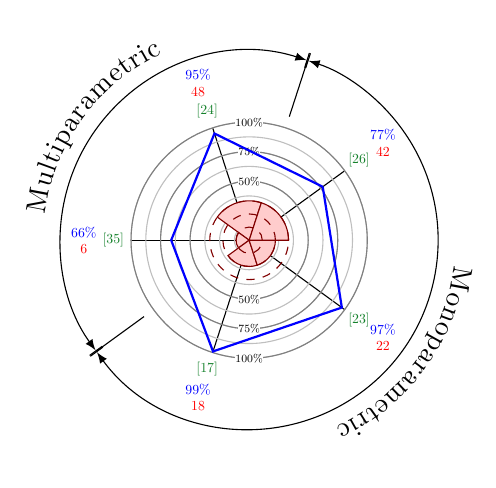
\begin{tikzpicture}[scale=.5,every node/.style={scale=0.5}]

\def\labels{
{\color{semiAuto}[24]},
{\color{semiAuto}[35]},
{\color{semiAuto}[17]},
{\color{semiAuto}[23]},
{\color{semiAuto}[26]}
}

\def\reward{95,66,99,97,77}
\def\dbSize{48,6,18,22,42}
\def\dbClass{3,1,2,2,3}		
\def\cZoom{3} 
\def\percentageLabelAngle{90}
\def\nbeams{5}
\pgfmathsetmacro\beamAngle{(360/\nbeams)}
\pgfmathsetmacro\halfAngle{(180/\nbeams)}
%\def\globalRotation{10}
\pgfmathsetmacro\globalRotation{\halfAngle}

% draw manual AOV results
%\filldraw[blue!15!white,even odd rule] (0,0) circle [radius={\cZoom*.852}] (0,0) circle [radius={\cZoom*.8}];
%\draw[thin,color=blue!50!white,dashed] (0,0) circle [radius={\cZoom*.852}] (0,0) circle [radius={\cZoom*.8}];

%\foreach \x in {.125,.25, ...,1} { \draw[thin]  (0,0) circle [radius={2*\x}]; }
% draw the radiants
\foreach \n  [count=\ni] in \labels
{
\pgfmathsetmacro\cAngle{{(\ni*(360/\nbeams))+\globalRotation}}
\draw	(\cAngle:{\cZoom*1.15})  node[fill=white] {\n};
\draw [thin] (0,0) -- (\cAngle:{\cZoom*1}) ;

}

% draw the % rings 
\foreach \x in {12.5,25, ...,100} 
\draw [thin,color=gray!50] (0,0) circle [radius={\cZoom*\x/100}];

\foreach \x in {50,75,100}
{ 
     \draw [thin,color=black!50] (0,0) circle [radius={\cZoom/100*\x}];
     \foreach \a in {0, 180} \draw ({\percentageLabelAngle+\a}:{\cZoom*0.01*\x}) node  [inner sep=0pt,outer sep=0pt,fill=white,font=\fontsize{8}{8.5}\selectfont]{$\x\%$};
}

% draw the path of the percentages
\def\aux{{\reward}}
\pgfmathsetmacro\origin{\aux[\nbeams-1]} 
\draw [blue, thick] (\globalRotation:{\cZoom*\origin/100}) \foreach \n  [count=\ni] in \reward { -- ({(\ni*(360/\nbeams))+\globalRotation}:{\cZoom*\n/100}) } ;

% label all the percentags
\foreach \n [count=\ni] in \dbSize 
{
	\pgfmathsetmacro\cAngle{{(\ni*(360/\nbeams))+\globalRotation}}
	\pgfmathsetmacro\nreward{\aux[\ni-1]}
	\draw (\cAngle:{\cZoom*1.4}) node[align=center] {{\color{blue}\nreward $\%$} \\ {\color{red}\n} };
} ;

% draw the database rose
\def\dbScale{\9}
\foreach \n [count=\ni] in \dbClass
\filldraw[fill=red!20!white, draw=red!50!black]
(0,0) -- ({\ni*(360/\nbeams)-\halfAngle+\globalRotation}:{\cZoom*\n/9}) arc ({\ni*(360/\nbeams)-\halfAngle+\globalRotation}:{\ni*(360/\nbeams)+\halfAngle+\globalRotation}:{\cZoom*\n/9}) -- cycle;
\foreach \x in {1,2,3}
\draw [thin,color=red!50!black,dashed] (0,0) circle [radius={\cZoom*\x/9}];

%% draw the domain of each class 
  \def\puta{	2/0/{Multiparametric},
  			3/2/{Monoparametric}}
%\def\putaa{  	2/9/{Other+ML},
%  			3/11/{ML},
%  			2/14/{ML+ACM}}

\foreach \numElm/\contadorQueNoSeCalcular/\name [count=\ni] in \puta
 {

 	\pgfmathsetmacro\initialAngle{(\contadorQueNoSeCalcular*\beamAngle)+\halfAngle+\globalRotation}
 	\pgfmathsetmacro\finalAngle  {((\numElm+\contadorQueNoSeCalcular)*\beamAngle)+\halfAngle+\globalRotation}
	\pgfmathsetmacro\l  {\cZoom*1.5+.3pt}
	\draw (\initialAngle:{\cZoom*1.6}) -- (\initialAngle:{\cZoom*1.1});
	\draw [ |<->|,>=latex] (\initialAngle:\l) arc (\initialAngle:\finalAngle:\l) ;    									 
	\pgfmathsetmacro\r  {\cZoom*1.5+.45pt}
    	{\draw [decoration={raise=4pt,text along path,  text={\name},text align={center}},decorate] (\finalAngle:\r) arc (\finalAngle:\initialAngle:\r);}
  }
%  
%   \foreach \numElm/\contadorQueNoSeCalcular/\name [count=\ni] in \putaa
% {
%
% 	\pgfmathsetmacro\initialAngle{(\contadorQueNoSeCalcular*\beamAngle)+\halfAngle+\globalRotation}
% 	\pgfmathsetmacro\finalAngle  {((\numElm+\contadorQueNoSeCalcular)*\beamAngle)+\halfAngle+\globalRotation}
%	\pgfmathsetmacro\l  {\cZoom*1.5+.3pt}
%	\draw (\initialAngle:{\cZoom*1.6}) -- (\initialAngle:{\cZoom*1.1});
%	\draw [ |<->|,>=latex] (\initialAngle:\l) arc (\initialAngle:\finalAngle:\l) ;    									 
%	\pgfmathsetmacro\r  {\cZoom*1.5+.7pt}
%    	{\draw [decoration={text along path, text={\name},text align={center}},decorate] (\initialAngle:\r) arc (\initialAngle:\finalAngle:\r);}    			 
%  }
        
\end{tikzpicture}
}
\hspace*{\fill}
\caption{Comparison of the results in terms of sensitivity (\ref{fig:sens15},\ref{fig:sens30}) and specificity (\ref{fig:spec15},\ref{fig:spec30}) for 1.5 and 3.0 Tesla \ac{mri} scanners. The {\color{blue}blue} value represents the metric and are graphically reported in the blue curve in the center of the figure. The {\color{red}red} value and areas correspond to the number of patients in the dataset. The numbers between brackets in {\color{semiAuto}green} correspond to the reference as reported in Tab. \ref{tab:sumpap}.}
\label{fig:sensspec}
\end{figure*}

Several metrics can be used in order to assess the performance of the classifier trained when tested on the test data. The techniques used for evaluation of the \ac{cad} system for \ac{cap} detection are summarized in Tab. \ref{tab:evatec}.

Using the classification approach previously presented, each voxel in the \ac{mri} image will be classified. Comparison with a ground-truth can give rise to a confusion matrix by counting true positive, true negative, false positive and false negative samples. From this analysis, different statistics can be extracted. 

The first statistic used is the accuracy which is computed as the ratio of true detection to the number of samples. However, depending on the strategy employed in the \ac{cad} work-flow, this statistic can be highly biased by a high number of true negative samples which will boost the accuracy score and does not represent the actual performance of the classifier.

That is why, the most common statistic computed are sensitivity and specificity which give a full overview of the performance of the classifier trained. Sensitivity is also called the true positive rate and is equal to the ratio of the true positive samples over the true positive added with the false negative samples as shown in Eq. \eqref{eq:sens}. Specificity is also named the true negative rate and is equal to the ratio of the true negative samples over the true negative added with the false positive samples as shown in Eq. \eqref{eq:spec}.

\begin{equation}
	SEN = \frac{TP}{TP+FN} \ ,
	\label{eq:sens}
\end{equation}

\begin{equation}
	SPE = \frac{TN}{TN+FP} \ .
	\label{eq:spec}
\end{equation}

These statistics gave rise to the \acf{roc} analysis. This analysis represents graphically the sensitivity as a function of (1 - specificity), which is in fact the false positive rate, by varying the discriminative threshold of the classifier. By varying this threshold, more true negative samples will be found but at the cost of detecting more false negatives. However, this fact is interesting in \ac{cad} since it is possible to obtain a high sensitivity and to ensure that no cancers were missed even if more false alarms have to be investigated. A statistic derived from \ac{roc} analysis is the \acf{auc} which corresponds to the area under the \ac{roc} and is a measure used to make comparisons between models.

The previous method could have been classified on pixel-based evaluation method. However, a cancer can be also considered as a region. The \acf{froc} extends the \ac{roc} analysis but to a region-based level. The same confusion matrix can be computed were the sample are not pixels any more but refer to a lesion. However, it is important to define what is a true positive sample in that case. Usually, a lesion is considered as a true positive sample if the region detected by the classifier overlaps ``sufficiently'' the one delineated in the ground-truth. However, ``Sufficiently'' is a subjective measure defined by each researcher and can correspond to one pixel only!!!

Finally, Dice's coefficient is sometimes computed which corresponds to the similarity between a detected lesion and its ground-truth. This coefficient consists of the ratio of twice the number of pixels in common to the sum of the pixels of the lesions in the ground-truth $GT$ and the output of the classifier $S$ defined as shown in Eq. \eqref{eq:dice}.

\begin{equation}
	Q_D = \frac{2 | GT \cap S |}{| GT | + | S |} \ .
	\label{eq:dice}
\end{equation}


\section{Discussion} \label{sec:discussion}

\subsection{Results reported}

%--------------------------------------------------------------------------------------------------------------------

\begin{figure}
\centering
%	\begin{tikzpicture}[scale=.5,every node/.style={scale=0.5}]
%
%\def\labels{
%{\color{semiAuto}[10]},
%{\color{semiAuto}[11]},
%{\color{semiAuto}[41]}
%}
%
%\def\reward{75,80,65}
%\def\dbSize{25,188,NA}
%\def\dbClass{1,3,0}		
%\def\cZoom{3} 
%\def\percentageLabelAngle{90}
%\def\nbeams{3}
%\pgfmathsetmacro\beamAngle{(360/\nbeams)}
%\pgfmathsetmacro\halfAngle{(180/\nbeams)}
%%\def\globalRotation{10}
%\pgfmathsetmacro\globalRotation{\halfAngle}
%
%% draw manual AOV results
%%\filldraw[blue!15!white,even odd rule] (0,0) circle [radius={\cZoom*.852}] (0,0) circle [radius={\cZoom*.8}];
%%\draw[thin,color=blue!50!white,dashed] (0,0) circle [radius={\cZoom*.852}] (0,0) circle [radius={\cZoom*.8}];
%
%%\foreach \x in {.125,.25, ...,1} { \draw[thin]  (0,0) circle [radius={2*\x}]; }
%% draw the radiants
%\foreach \n  [count=\ni] in \labels
%{
%\pgfmathsetmacro\cAngle{{(\ni*(360/\nbeams))+\globalRotation}}
%\draw	(\cAngle:{\cZoom*1.15})  node[fill=white] {\n};
%\draw [thin] (0,0) -- (\cAngle:{\cZoom*1}) ;
%
%}
%
%% draw the % rings 
%\foreach \x in {12.5,25, ...,100} 
%\draw [thin,color=gray!50] (0,0) circle [radius={\cZoom*\x/100}];
%
%\foreach \x in {50,75,100}
%{ 
%     \draw [thin,color=black!50] (0,0) circle [radius={\cZoom/100*\x}];
%     \foreach \a in {0, 180} \draw ({\percentageLabelAngle+\a}:{\cZoom*0.01*\x}) node  [inner sep=0pt,outer sep=0pt,fill=white,font=\fontsize{8}{8.5}\selectfont]{$\x\%$};
%}
%
%% draw the path of the percentages
%\def\aux{{\reward}}
%\pgfmathsetmacro\origin{\aux[\nbeams-1]} 
%\draw [blue, thick] (\globalRotation:{\cZoom*\origin/100}) \foreach \n  [count=\ni] in \reward { -- ({(\ni*(360/\nbeams))+\globalRotation}:{\cZoom*\n/100}) } ;
%
%% label all the percentags
%\foreach \n [count=\ni] in \dbSize 
%{
%	\pgfmathsetmacro\cAngle{{(\ni*(360/\nbeams))+\globalRotation}}
%	\pgfmathsetmacro\nreward{\aux[\ni-1]}
%	\draw (\cAngle:{\cZoom*1.4}) node[align=center] {{\color{blue}\nreward $\%$} \\ {\color{red}\n} };
%} ;
%
%% draw the database rose
%\def\dbScale{\9}
%\foreach \n [count=\ni] in \dbClass
%\filldraw[fill=red!20!white, draw=red!50!black]
%(0,0) -- ({\ni*(360/\nbeams)-\halfAngle+\globalRotation}:{\cZoom*\n/9}) arc ({\ni*(360/\nbeams)-\halfAngle+\globalRotation}:{\ni*(360/\nbeams)+\halfAngle+\globalRotation}:{\cZoom*\n/9}) -- cycle;
%\foreach \x in {1,2,3}
%\draw [thin,color=red!50!black,dashed] (0,0) circle [radius={\cZoom*\x/9}];
%
%%% draw the domain of each class 
%  \def\puta{	3/0/{Multiparametric}}
%%\def\putaa{  	2/9/{Other+ML},
%%  			3/11/{ML},
%%  			2/14/{ML+ACM}}
%
%\foreach \numElm/\contadorQueNoSeCalcular/\name [count=\ni] in \puta
% {
%
% 	\pgfmathsetmacro\initialAngle{(\contadorQueNoSeCalcular*\beamAngle)+\halfAngle+\globalRotation}
% 	\pgfmathsetmacro\finalAngle  {((\numElm+\contadorQueNoSeCalcular)*\beamAngle)+\halfAngle+\globalRotation}
%	\pgfmathsetmacro\l  {\cZoom*1.5+.3pt}
%	\draw (\initialAngle:{\cZoom*1.6}) -- (\initialAngle:{\cZoom*1.1});
%	\draw [ |<->|,>=latex] (\initialAngle:\l) arc (\initialAngle:\finalAngle:\l) ;    									 
%	\pgfmathsetmacro\r  {\cZoom*1.5+.45pt}
%    	{\draw [decoration={raise=4pt,text along path,  text={\name},text align={center}},decorate] (\finalAngle:\r) arc (\finalAngle:\initialAngle:\r);}
%  }
%%  
%%   \foreach \numElm/\contadorQueNoSeCalcular/\name [count=\ni] in \putaa
%% {
%%
%% 	\pgfmathsetmacro\initialAngle{(\contadorQueNoSeCalcular*\beamAngle)+\halfAngle+\globalRotation}
%% 	\pgfmathsetmacro\finalAngle  {((\numElm+\contadorQueNoSeCalcular)*\beamAngle)+\halfAngle+\globalRotation}
%%	\pgfmathsetmacro\l  {\cZoom*1.5+.3pt}
%%	\draw (\initialAngle:{\cZoom*1.6}) -- (\initialAngle:{\cZoom*1.1});
%%	\draw [ |<->|,>=latex] (\initialAngle:\l) arc (\initialAngle:\finalAngle:\l) ;    									 
%%	\pgfmathsetmacro\r  {\cZoom*1.5+.7pt}
%%    	{\draw [decoration={text along path, text={\name},text align={center}},decorate] (\initialAngle:\r) arc (\initialAngle:\finalAngle:\r);}    			 
%%  }
%        
%\end{tikzpicture}
%\caption{Comparison in terms of \ac{froc} of the methods using data from 3.0 Tesla \ac{mri} scanner. The blue value represent the metric and are graphically reported in the blue curve in the center of the figure. The red value correspond to the number of patients in the dataset and is also reported in the center of the figure. The numbers between brackets correspond to the reference as reported in Tab. \ref{tab:sumpap}.}
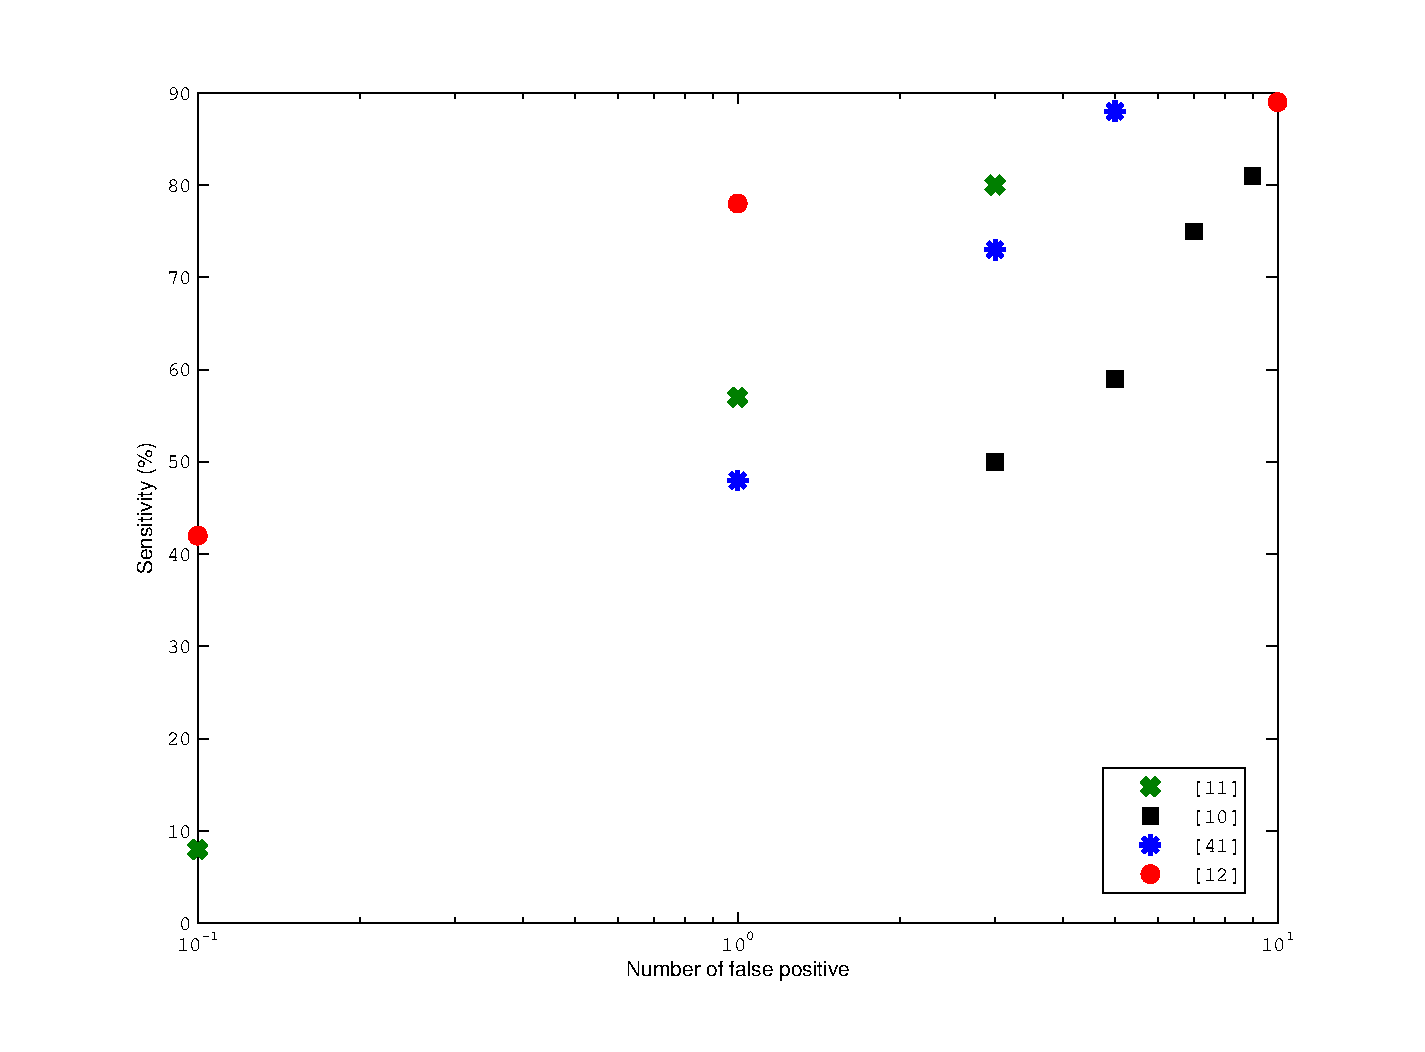
\includegraphics[width=1\linewidth]{09_discussion/figures/froc.eps}
\caption{Comparison in terms of \ac{froc} of the methods using data from 3.0 Tesla \ac{mri} scanner.}
\label{fig:froc}
\end{figure}

As discussed previously in Sect. \ref{subsubsec:eval}, different metrics have been used to report results. A comparison of the different methods reviewed is given depending on the metric used in field of research and also the type of \ac{mri} scanner used (cf., 1.5 \textit{versus} 3.0 Tesla). For each field, the \textit{best performances} obtained in each study were reported in these figures.

The results given in terms of \ac{auc}-\ac{roc} are depicted in Fig.~\ref{fig:auc}. The results vary between $71\%$ and $97\%$ for some experiments with a 1.5 Tesla \ac{mri} scanner and $77\%$ and $95\%$ with a 3.0 Tesla \ac{mri} scanner. 

The results in regard of sensitivity and specificity are reported in Fig.~\ref{fig:sensspec}. In the case that the data were collected with a 1.5 Tesla \ac{mri} scanner, the sensitivity ranges from $74\%$ to $100\%$ and the specificity from $43\%$ to $93\%$. For the experiments carried out with a 3.0 Tesla \ac{mri} scanner, the sensitivity varies from $60\%$ to $90\%$ and the specificity from $66\%$ to $99\%$.

Four studies also use \ac{froc} analysis to report their results and are reported in Fig.~\ref{fig:froc}.

%We would like to emphasize the fact that the results obtained from these different experiments cannot be fairly compared. Different datasets were used implying different complexity involved and different sets of input parameters during the data acquisition. To our mind, the only way to provide a real and fair comparison would be to provide a common working dataset where those algorithms could be tested.

\subsection{Comparison}

{\color{red} We would like to stress the following findings drawn during the review of the different studies:

\begin{enumerate}
	\item Quantitatively, it is difficult to make a fair comparison between the different studies reviewed. Different factors come into play to elucidate this fact. Mainly a lack of standardization can be pointed out in regard to experimental evaluation: (i) different datasets are used during the evaluation of the frameworks developed disabling a comparison inter-studies. The same conclusion has been recently drawn by \cite{Litjens2014} supporting this argument; (ii) the experimental results are not reported with a common metric which leads to the inability to compare the different studies.
	
	\item \label{here} However, multiple studies reported some performance improvements using multi-parametric imaging techniques instead of mono-parametric imaging techniques. Considering only the most recent studies proposing \ac{cade}-\ac{cadx} frameworks, the following results can be highlighted. 	
	\cite{Viswanath2011} obtained an \ac{auc} of $77\%$ using an ensemble learning approach combining the features from the three modalities \ac{t2w}-\ac{dce}-\ac{dw} \ac{mri}, while the results obtained as standalone modality were ranging from $62\%$ to $65\%$. 	
	\cite{Tiwari2013} drawn similar conclusions by using \ac{t2w} and \ac{mrsi} modalities as both in standalone and multi-parametric framework with an improved \ac{auc} from $57\%$-$76\%$ to $85\%$. 	
	The most recent work of \cite{Litjens2014} obtained an improved \ac{auc} metric from $71\%$-$76\%$ considering each modality separately (e.g., \ac{t2w}-\ac{dce}-\ac{dw} \ac{mri}) to $89\%$ in their multi-parametric framework.
	
		\item The studies comparing particular combination of more than one modality give rise to the same fact (\cite{Ozer2010,Litjens2011,Liu2013,Litjens2014}): using three modalities lead to better performances than using any combination of two modalities. 
	
	\item Unlike the previous remark \ref{here}, no straightforward conclusions can be given regarding the performances of each modality in a standalone framework. The modality being processed by different methods, it does not allow us to conclude if a modality by itself is more suited than another. However, we were able to distinguish some interesting trends which deserves the attention of the community. \cite{Tiwari2009a,Tiwari2012,Tiwari2013} observed that \ac{mrsi} is a more suitable modality than \ac{t2w} to highlight cancers. Moreover, \ac{adc} maps have shown a better discriminative power than \ac{t2w} as well (\cite{Langer2009,Viswanath2011,Peng2013}). Lately, \cite{Litjens2014} observed that \ac{dw} modality was more suitable than both \ac{dce} and \ac{t2w} to distinguish \ac{cap} in their \ac{cadx} system. 

	\item Furthermore, multi-parametric has attracted the attention of both radiologists and computer vision researchers. Indeed, pioneer research groups included new modalities over years when at the same time, new research groups directly introduced multi-parametric \ac{cad} systems. These facts lead us to think that \ac{cap} researches will benefit from multi-parametric imaging techniques.

	\item When focusing on the different modalities used, it can be pointed out that no research reported the use of all modalities in a single framework: \ac{mrsi} is usually used as a standalone modality and never combined with the three remaining. Nevertheless, this modality has shown some overall good performances at the price of a lower resolution as well as an acquisition time. Moreover, \ac{mrsi} analysis is more complex in comparison with the other modalities. To our mind, \ac{mrsi} could contribute in a multi-parametric framework and should be fused with the other modalities.

	\item Lately, three studies (\cite{Viswanath2012,Litjens2012,Litjens2014}) focused on developing a region-based classification in which \ac{pz} and \ac{cg} will be analysed separately instead of jointly. The results provided seem to be promising and which indicates that this strategy should be further investigated.
	
	\item Recent studies are using quantitative features rather than only \ac{si} as input to ``image classification''. Even if the studies do not allow us to perform a direct comparison, it seems that these quantitative features provide decorrelate information in regard with \ac{si} features and should lead to better performances when combined all together. 
	
	\item Regarding the methods used in the ``image regularisation'' (cf., pre-processing, segmentation and registration), it is particularly difficult to distinguish the benefit of a method over another since none of the studies focus on making comparison of these processing stages. The focus is usually entirely based on the ``image classification'' framework where different methods are directly compared. Note that the performances of a classifier are highly linked with the features vector in input (cf., discriminative power of the features, correlation of the features, etc.), it is not appropriate to affirm that a machine learning method is outperforming another. However, we could identify a trend in which \ac{svm} as well as ensemble learning classifiers (e.g., AdaBoost, GentleBoost and random forest) seem to perform better than neural network, \ac{lda} or Naive Bayes.
	
	\item We would like to draw the attention of the reader on the feature extraction/selection stage. This processing could reduce the complexity and also find a better feature space for classification. However, few studies are performing such approaches. \cite{Niaf2011,Niaf2012} are successfully applying a scheme to reduce the number of dimensions by selecting the most discriminative features. It allows them to obtain improved performances compared with a classification performed with their initial feature vector. Another group of studies also applied different feature extraction methods (\cite{Viswanath2008a,Viswanath2008,Viswanath2012,Tiwari2007,Tiwari2008,Tiwari2009,Tiwari2010,Tiwari2012,Tiwari2013}). In these specific cases, no comparison is performed against non-dimension reduction case but it is likely that the results obtained are improved.
\end{enumerate}}

\subsection{General discussion}

This review leads to some general discussions which could direct to future avenues for research. As previously mentioned, no open multi-parametric dataset is currently available. This fact leads to an impossibility to fairly compare the different algorithms designed over years. Also, the availability of a full multi-parametric \ac{mri} dataset, could lead to the development of algorithms which use all the different modalities currently available. Recalling Tab. \ref{tab:sumpap}, it can be noted that none of the current works provides a solution using at the same time the four different modalities. Also, all the algorithms are focused on one type of scanner only, either 1.5 Tesla and 3.0 Tesla. A dataset including both these types of imaging could allow development of more generic algorithms.

Analysing the different stages of the \ac{cad} work-flow, it is seen that the actual \ac{cad} systems do not include all the different pre-processing steps. It could be interesting to evaluate the improvement using these pre-processing steps on the final results obtained after the classification. Regarding segmentation and registration of the prostate, \ac{cad} systems could greatly benefit from specific research in these areas which could lead to a better automation of those systems. Moreover, other methods specific to segmentation and registration which are not actually used in \ac{cad} systems could also perform better than the ones currently used in \acp{cad}.

Regarding the classification framework, it seems that the current well-known pattern recognition methods have been widely studied. However, more investigations should be carried out regarding the feature detection stage. Lately, histogram-based features have shown good capabilities in the field of computer vision and could be further investigated. Only one study by \cite{Liu2013} used some of these features.

An important point allowing a fair comparison between methods resides in the fact that no universal evaluation model and metric has been defined by the research community allowing such comparison. Usually, it is quite common to choose an evaluation model which fits the dataset limitations, usually the size. Regarding the evaluation, the community should agree on a standard metric to measure the performance of the algorithms designed.

Finally, we would like to focus the attentions of the reader on the availability of a multi-parametric dataset \ac{mri} provided by the authors of this review, from a 1.5 Tesla General Electric scanner and a 3.0 Tesla Siemens scanner. This dataset will be available at the following website address: \texttt{http://visor.udg.edu/dataset}. The dataset is composed of the four modalities discussed in this review with their corresponding ground-truth images. For each scanner type, each subset will be composed of twenty patients with cancerous lesions and ten healthy patients. In addition of the repository activity, this website will aim at providing comparison between algorithms developed by the research community.

\section{Conclusion} \label{sec:conclusion}

This review presented an overview and gave a staging of the research related to \ac{cad} development for \ac{cap} using multi-parametric \ac{mri} data. We aimed at providing background information regarding multi-parametric \ac{mri} imaging techniques. A work-flow describing the \ac{cad} stages were proposed. The methods used in the literature for each of this stage were reviewed. The results of the available \ac{cad} systems were briefly reviewed. Subsequently, an insight discussion were given to conclude this survey. 

\section{Acknowledgement} \label{sec:acknowledgement}

We would like to acknowledge Sharad Nagappa for all the discussions and his precious advices regarding the redaction of this current review.


%%%%%%%%%%%%%%%%%%%%%%%%%%%%%%%%%%%%%%%%%%%%%%%%%

%%%%%%%%%%%%%%%%%%%%%%%%%%%%%%%%%%%%%%%%%%%%%%%%%
%%% BIBTEX AND BIBLIOGRAPHY START HERE

\section*{References}

\bibliographystyle{elsarticle-num}
\bibliography{bibtex/literature_review.bib}

%%%%%%%%%%%%%%%%%%%%%%%%%%%%%%%%%%%%%%%%%%%%%%%%%

\clearpage

\begin{figure*}
  \centering

  % Define block styles used later

  \tikzstyle{module}=[draw, draw=blue!80, text width=10em, 
  text centered, minimum height=5em, minimum width = 15em, drop shadow, rounded corners,
  fill=blue!30]
  
  \tikzstyle{vecArrow} = [thick, decoration={markings,mark=at position
    1 with {\arrow[semithick]{open triangle 60}}},
  double distance=1.4pt, shorten >= 5.5pt,
  preaction = {decorate},
  postaction = {draw,line width=1.4pt, white,shorten >= 4.5pt}]

  % Define distances for bordering
  \def\blockdist{1.5}
  \def\edgedist{2.5}

  \begin{tikzpicture}[node distance=3cm,thick,scale=0.6, every node/.style={scale=0.6},path image/.style={
      path picture={
        \node at (path picture bounding box.center) {
          \includegraphics[width=1cm]{#1}
        };}}]
    \tikzstyle{conefill} = [path image=,fill opacity=0.8]
    \node[module=above:pre] (pre) at (4.5,-2.6) {\Large Pre-processing};
    \node[module,below of=pre] (seg) {\Large Segmentation};
    \node[module,below of=seg] (reg) {\Large Registration};

    \path[->,dashed] (seg.west) edge [bend right=70] node {} (reg.west);
    \path[->,dashed] (reg.east) edge [bend right=70] node {} (seg.east);

    \draw[->] (pre)--(seg);
    \draw[->] (seg)--(reg);

    \begin{pgfonlayer}{background}
      \path (pre.west |- pre.north)+(-0.9,1.0+\blockdist) node (a) {};
      \path (reg.east |- reg.south)+(+0.9,-0.5) node (b) {};
      
      \path[fill=blue!10,rounded corners, draw=blue!20, dashed] (a) rectangle (b);
    \end{pgfonlayer}
    
    \path (pre.north) +(0,+\blockdist) node (bgreg) {\Large Image regularization};

    \begin{scope}[node distance=10cm]
      \node[module] (det) [below right=0cm and 3cm of pre] {\Large Features detection};
    \end{scope}
    \begin{scope}[node distance=3.5cm]
      \node[module,above of=det] (roi) {\Large ROIs\\detection/selection};
    \end{scope}
    \node[module,below of=det] (sel) {\Large Features\\selection/extraction};
    \node[module,below of=sel] (cla) {\Large Features\\classification/fusion};

    \draw[->] (roi)--(det);
    \draw[->] (det)--(sel);
    \draw[->] (sel)--(cla);

    \begin{pgfonlayer}{background}
      \path (roi.west |- roi.north)+(-0.25,0.8) node (c) {};
      \path (roi.east |- roi.south)+(+0.25,-0.25) node (d) {};
      
      \path[fill=blue!20,rounded corners, draw=blue!25, dashed] (c) rectangle (d);
    \end{pgfonlayer}

    \path (roi.west |- roi.north) +(.6,0.4) node (bgfea) {\Large \textbf{CADe}};

    \begin{pgfonlayer}{background}
      \path (det.west |- det.north)+(-0.25,0.8) node (c) {};
      \path (cla.east |- cla.south)+(+0.25,-0.25) node (d) {};
      
      \path[fill=blue!20,rounded corners, draw=blue!25, dashed] (c) rectangle (d);
    \end{pgfonlayer}

    \path (roi.west |- det.north) +(.6,0.4) node (bgfea) {\Large \textbf{CADx}};     

    % Define the place where the arrow should start anf finish
    \path (seg.east |- seg.north)+(+0.9,0) node (e) {};
    \path (sel.west |- seg.north)+(-0.8,0) node (f) {};

    \draw[double distance =3pt,preaction={-triangle 90,thin,draw,shorten >=-1mm}] (e) -- (f) node[midway,above] {\Large Regularized data};

    \begin{scope}[yshift=34,xshift=-86]
      \transparent{0.6}\draw[path image=12_figures/figures/tikzimage/t2.eps] (0,0) rectangle (1.0,1.0);
    \end{scope}

    \begin{scope}[yshift=31,xshift=-83]
      \transparent{0.6}\draw[path image=12_figures/figures/tikzimage/t2.eps] (0,0) rectangle (1.0,1.0);
    \end{scope}

    \begin{scope}[yshift=28,xshift=-80]
      \transparent{0.8}\draw[path image=12_figures/figures/tikzimage/t2.eps] (0,0) rectangle (1.0,1.0);
      \path (0,0)+(-1.5,0.3) node {\Large T$_2$-W MRI};
    \end{scope}

    \begin{scope}[yshift=-33,xshift=-86]
      \transparent{0.6}\draw[path image=12_figures/figures/tikzimage/t2.eps] (0,0) rectangle (1.0,1.0);
    \end{scope}

    \begin{scope}[yshift=-36,xshift=-83]
      \transparent{0.6}\draw[path image=12_figures/figures/tikzimage/t2.eps] (0,0) rectangle (1.0,1.0);
    \end{scope}

    \begin{scope}[yshift=-39,xshift=-80]
      \transparent{0.8}\draw[path image=12_figures/figures/tikzimage/t2.eps] (0,0) rectangle (1.0,1.0);
      \path (0,0)+(-1.2,0.3) node {\Large T$_2$ map};
    \end{scope}

    \begin{scope}[yshift=-100,xshift=-86]
      \transparent{0.6}\draw[path image=12_figures/figures/tikzimage/dce.eps] (0,0) rectangle (1.0,1.0);
    \end{scope}

    \begin{scope}[yshift=-103,xshift=-83]
      \transparent{0.6}\draw[path image=12_figures/figures/tikzimage/dce.eps] (0,0) rectangle (1.0,1.0);
    \end{scope}

    \begin{scope}[yshift=-106,xshift=-80]
      \transparent{0.8}\draw[path image=12_figures/figures/tikzimage/dce.eps] (0,0) rectangle (1.0,1.0);
      \path (0,0)+(-1.5,0.3) node {\Large DCE MRI};
    \end{scope}

    \begin{scope}[yshift=-167,xshift=-86]
      \transparent{0.6}\draw[path image=12_figures/figures/tikzimage/dwi1.eps] (0,0) rectangle (1.0,1.0);
    \end{scope}

    \begin{scope}[yshift=-170,xshift=-83]
      \transparent{0.6}\draw[path image=12_figures/figures/tikzimage/dwi1.eps] (0,0) rectangle (1.0,1.0);
    \end{scope}

    \begin{scope}[yshift=-173,xshift=-80]
      \transparent{0.8}\draw[path image=12_figures/figures/tikzimage/dwi1.eps] (0,0) rectangle (1.0,1.0);
      \path (0,0)+(-1.5,0.3) node {\Large DW MRI};
    \end{scope}

    \begin{scope}[yshift=-234,xshift=-86]
      \transparent{0.6}\draw[path image=12_figures/figures/tikzimage/adc.eps] (0,0) rectangle (1.0,1.0);
    \end{scope}

    \begin{scope}[yshift=-237,xshift=-83]
      \transparent{0.6}\draw[path image=12_figures/figures/tikzimage/adc.eps] (0,0) rectangle (1.0,1.0);
    \end{scope}

    \begin{scope}[yshift=-240,xshift=-80]
      \transparent{0.8}\draw[path image=12_figures/figures/tikzimage/adc.eps] (0,0) rectangle (1.0,1.0);
      \path (0,0)+(-1.5,0.3) node {\Large ADC};
    \end{scope}

    \begin{scope}[yshift=-301,xshift=-86]
      \transparent{0.6}\draw[path image=12_figures/figures/tikzimage/mrsi.eps] (0,0) rectangle (1.0,1.0);
    \end{scope}

    \begin{scope}[yshift=-304,xshift=-83]
      \transparent{0.6}\draw[path image=12_figures/figures/tikzimage/mrsi.eps] (0,0) rectangle (1.0,1.0);
    \end{scope}

    \begin{scope}[yshift=-307,xshift=-80]
      \transparent{0.8}\draw[path image=12_figures/figures/tikzimage/mrsi.eps] (0,0) rectangle (1.0,1.0);
      \path (0,0)+(-1,0.3) node {\Large MRSI};
    \end{scope}

    \path (pre.west |- roi.north)+(-3.5,1.0+\blockdist) node (g) {};
    \path (reg.west |- cla.south)+(-3.5,-0.5) node (h) {};

    \draw[decorate,decoration={brace,raise=6pt,amplitude=10pt}, thick]
    (g)--(h) ;
    
    \path (seg.west |- seg.north)+(-2.5,0) node (i) {};
    \path (seg.west |- seg.north)+(-0.9,0) node (j) {};
    
    \draw[double distance =3pt,preaction={-triangle 90,thin,draw,shorten >=-1mm}] (i) -- (j);   

    \path (sel.east |- seg.north)+(2,0) node (k) {};
    \path (sel.east |- seg.north)+(0.5,0) node (l) {};
    
  \end{tikzpicture}
  \caption{Common \ac{cad} framework based on \ac{mri} images used to detect \ac{cap}.}
  \label{fig:wkfcad}
\end{figure*}

\begin{figure*}
  \centering
  \hspace*{\fill}
  \subfigure[\ac{t2w}-\ac{mri} slice of an healthy prostate acquire with a 1.5 Tesla \ac{mri}. The blue contour represents the \ac{cg} while the \ac{pz} corresponds to the green contour.]{\label{subfig:t2whealthy}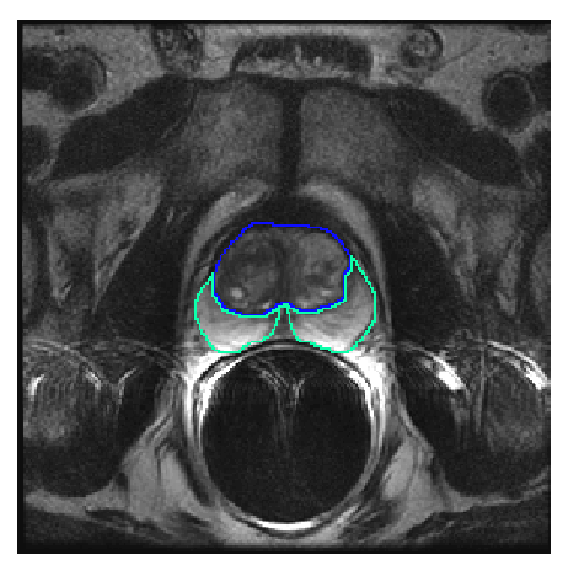
\includegraphics[width=0.3\linewidth]{12_figures/figures/t2w/t2w_healthy.eps}} \hfill
  \subfigure[\ac{t2w}-\ac{mri} slice of a prostate with a \ac{cap} highlighted in the \ac{pz} using a 3.0 Tesla \ac{mri} scanner.]{\label{subfig:t2wcancerpz}\includegraphics[width=0.3\linewidth]{12_figures/figures/t2w/t2w_cancer_pz.eps}} \hfill
  \subfigure[\ac{t2w}-\ac{mri} slice of a prostate with a \ac{cap} highlighted in the \ac{cg} using a 3.0 Tesla \ac{mri} scanner.]{\label{subfig:t2wcancercg}\includegraphics[width=0.3\linewidth]{12_figures/figures/t2w/t2w_cancer_cg.eps}}
  \hspace*{\fill}
  \caption{Rendering of \ac{t2w}-\ac{mri} prostate image with both 1.5 and 3.0 Tesla \ac{mri} scanner.}
  \label{fig:t2w}
\end{figure*}

\begin{figure*}
  \centering
  \hspace*{\fill}
  \subfigure[]{\label{subfig:t1w}\includegraphics[width=0.35\linewidth]{12_figures/figures/dce/slice.eps}} \hfill
  \subfigure[]{\label{subfig:dce}\includegraphics[width=0.35\linewidth]{12_figures/figures/dce/dce_cancer_healthy.eps}}
  \hspace*{\fill}
  \caption{Illustration of: \subref{subfig:t1w} \ac{t1w}-\ac{mri} image and \subref{subfig:dce} typical enhancement signals observed in \ac{dce}-\ac{mri} analysis collected with a 3.0 Tesla \ac{mri} scanner. The red curve is typical from \ac{cap} while the green curve is characteristic of healthy tissue.}
  \label{fig:dceana}
\end{figure*}

\begin{figure}
  \centering
  \hspace*{\fill}
  \subfigure[]{\label{subfig:dwi}\includegraphics[height=0.15\textheight]{12_figures/figures/dwi/dwi_cancer.eps}} \hfill
  \subfigure[]{\label{subfig:adc}\includegraphics[height=0.15\textheight]{12_figures/figures/dwi/adc_cancer.eps}}
  \hspace*{\fill}
  \caption{Illustration of: \subref{subfig:dwi} \ac{dw}-\ac{mri} and \subref{subfig:adc} \ac{adc} map. The signal intensity corresponding to cancer are inversely correlated on these two types of imaging techniques. The cancer is highlighted in red.}
  \label{fig:dwi}
\end{figure}

\begin{figure*}
  \centering
  \hspace*{\fill}
  \subfigure[]{\label{subfig:mrsihea}\includegraphics[width=0.45\linewidth]{12_figures/figures/mrsi/mrsi_healthy.eps}} \hfill
  \subfigure[]{\label{subfig:mrsican}\includegraphics[width=0.45\linewidth]{12_figures/figures/mrsi/mrsi_cancer.eps}}
  \hspace*{\fill}
  \caption{Illustration of an \ac{mrsi} spectrum both \subref{subfig:mrsihea} healthy and \subref{subfig:mrsican} cancerous voxel with a 3.0 Tesla \ac{mri}. The highlighted areas corresponds to the related concentration of the metabolites which is computed by integrating the area under each peak. Acronyms: Choline (Cho), Spermine (Spe), Creatine (Cr) and Citrate (Cit).}
  \label{fig:mrsi}
\end{figure*}

% \begin{figure}
%   \centering
%   \hspace*{\fill}
%   \subfigure[]{\label{subfig:bladder} 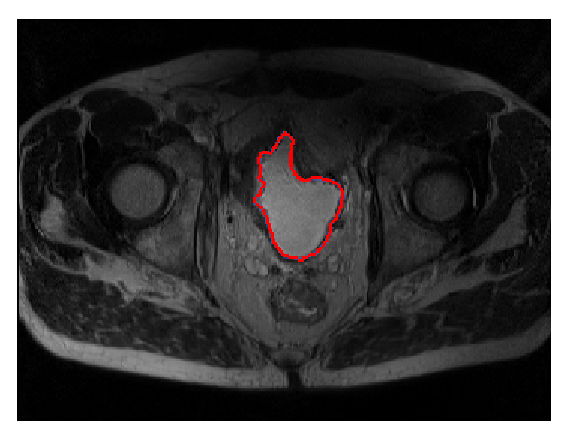
\includegraphics[width=0.3\linewidth]{12_figures/figures/niaf/t2w_bladder.eps}} \hfill
%   \subfigure[]{\label{subfig:arteries} \includegraphics[width=0.3\linewidth]{12_figures/figures/niaf/t1w_arteries.eps}}
%   \hspace*{\fill}
%   \caption{Illustration of the two organs, \subref{subfig:bladder} the bladder and \subref{subfig:arteries} the femoral arteries which are used in \cite{Niaf2011,Niaf2012} to normalize \ac{t2w} and \ac{t1w} \ac{mri} images.}
%   \label{fig:niaf}
% \end{figure}

% \begin{figure}
% \centering
%   \hspace*{\fill}
%   \subfigure[]{\label{fig:phase} \includegraphics[height=0.23\textheight]{12_figures/figures/phase/phase.eps}} \hfill
%   \subfigure[]{\label{fig:waterfat} \includegraphics[height=0.23\textheight]{12_figures/figures/water/water_fat.eps}}
%   \hspace*{\fill}
%   \caption{\subref{fig:phase} Illustration of frequency and phase misalignment in an \ac{mrsi} spectra acquired with a 3.0 Tesla \ac{mrsi} scanner. Focusing on the phase misalignment, note the distortion of the signal specially visible for the water (cf., around 5.1 ppm) and citrate (cf., around 3 ppm) peaks. Regarding the frequency misalignment, the water peak is known to be aligned at 4.65 ppm. However, it can observed that this peak is occurring around 5.1 ppm; \subref{fig:waterfat} Illustration of the residues of water and fat even after their suppression during the acquisition protocol. The acquisition was carried out with a 3.0 Tesla \ac{mri}.}
%   \label{fig:mrsispe}
% \end{figure}

\begin{figure}
  \centering

  % Define block styles used later

  \tikzstyle{module}=[draw, draw=blue!80, text width=10em, 
  text centered, minimum height=5em, minimum width = 10em, drop shadow, rounded corners,
  fill=blue!30]
  
  \tikzstyle{vecArrow} = [thick, decoration={markings,mark=at position
    1 with {\arrow[semithick]{open triangle 60}}},
  double distance=1.4pt, shorten >= 5.5pt,
  preaction = {decorate},
  postaction = {draw,line width=1.4pt, white,shorten >= 4.5pt}]

  % Define distances for bordering
  \def\blockdist{1.5}
  \def\edgedist{2.5}

  \definecolor{darkblue}{rgb}{0.2,0.2,0.6}
  \definecolor{darkred}{rgb}{0.6,0.1,0.1}
  \definecolor{darkgreen}{rgb}{0.2,0.6,0.2}

  \def\arrow{
    (10.75:1.1) -- (6.5:1) arc (6.25:120:1) [rounded corners=0.5] --
    (120:0.9) [rounded corners=1] -- (130:1.1) [rounded corners=0.5] --
    (120:1.3) [sharp corners] -- (120:1.2) arc (120:5.25:1.2)
    [rounded corners=1] -- (10.75:1.1) -- (6.5:1) -- cycle
  }

  \tikzset{
    ashadow/.style={opacity=.25, shadow xshift=0.07, shadow yshift=-0.07},
  }

  \def\arrows[#1]{         
    \begin{scope}[scale=#1]
      \node[align=center] at (0,0) {\Huge{ Loop } \\ \Huge{ until matching } };  
      
      \draw[color=darkred, %
      drop shadow={ashadow, color=red!60!black}] \arrow;

      \draw[color=darkgreen, bottom color=green!60!black, top color=green!30, %
      drop shadow={ashadow, color=green!60!black}] [rotate=120] \arrow;

      \draw[color=darkblue, right color=blue!60, left color=blue!30, %
      drop shadow={ashadow, color=blue!60!black}] [rotate=240] \arrow;

      % to hide the green shadow
      \draw[color=darkred, left color=red!60, right color=red!30] \arrow;
    \end{scope}
  }

  \begin{tikzpicture}[node distance=3cm,thick,scale=0.5, every node/.style={scale=0.5},path image/.style={
      path picture={
        \node at (path picture bounding box.center) {
          \includegraphics[width=1cm]{#1}
        };}}]
    \tikzstyle{conefill} = [path image=,fill opacity=0.8]

    \node (t2w) at (0,0)	{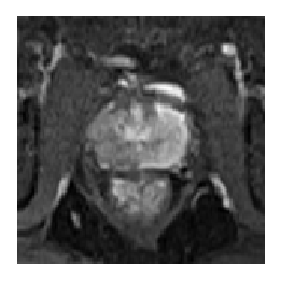
\includegraphics[width=1.5cm]{12_figures/figures/tikzimage/dce.eps}};
    \begin{scope}[node distance=1.2cm]
      \node[below of=t2w] (cap1) {\Large Fixed};
    \end{scope}
    \begin{scope}[node distance=6cm]
      \node[below of=t2w] 	(dce) 			{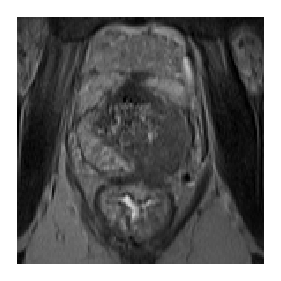
\includegraphics[width=1.5cm]{12_figures/figures/tikzimage/t2.eps}};
      \begin{scope}[node distance=1.2cm]
        \node[below of=dce] (cap2) {\Large Moving};
      \end{scope}
    \end{scope}

    \begin{scope}[node distance=5.5cm]
      \node[module,right of=t2w] (sim) {\Large Similarity \\ measure};
    \end{scope}
    \begin{scope}[node distance=3cm]
      \node[module,below of=sim] (int) {\Large Interpolator};
      \node[module,below of=int] (tra) {\Large Transform};
    \end{scope}

    \draw[line width=1mm,draw=blue!30,->] (t2w)--(sim);  
    \draw[line width=1mm,draw=blue!30,->] (dce)--(tra); 

    \begin{scope}[node distance=9cm]
      \node[module,right of=sim] (opt) {\Large Optimizer};
    \end{scope}

    \draw[draw=blue,->,line width=.5mm] (tra)--(int);
    \draw[draw=blue,->,line width=.5mm] (int)--(sim);
    \draw[draw=blue,->,line width=.5mm] (sim)--(opt) node[midway,above] {\Large Similarity} node[midway,below] {\Large metric};
    \draw[draw=blue,->,line width=.5mm] (opt)|-(tra); 

    \begin{pgfonlayer}{background}
      \path (sim.west |- sim.north)+(-0.5,.5) node (a) {};
      \path (opt.east |- tra.south)+(+0.5,-0.5) node (b) {};
      
      \path[fill=blue!10,rounded corners, draw=blue!20, dashed] (a) rectangle (b);
    \end{pgfonlayer} 

    \begin{scope}[node distance=5cm]
      \node[right of=int] (arr) {
        \begin{tikzpicture}
          \arrows[1.9];
        \end{tikzpicture}
      };
    \end{scope}
  \end{tikzpicture}
  \caption{Typical framework involved to solve the registration problem.}
  \label{fig:frareg}
\end{figure}

% \begin{figure}
%   \centering
%   \hspace*{\fill}
%   \subfigure[]{\label{subfig:histoalgn} 
\includegraphics[width=0.2\textwidth]{12_figures/figures/histogram/jointhistoalg.eps}} \hfill
%   \subfigure[]{\label{subfig:histomisalgn} 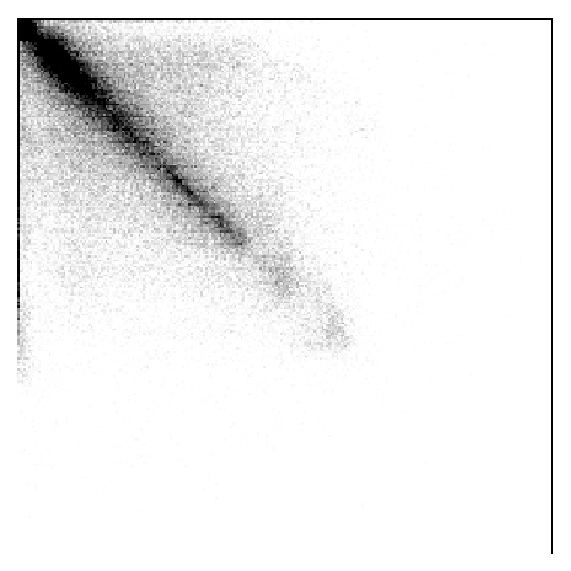
\includegraphics[width=0.2\textwidth]{12_figures/figures/histogram/jointhistomisal.eps}}
%   \hspace*{\fill}
%   \caption{Difference observed in joint histogram between aligned \subref{subfig:histoalgn} and misaligned \subref{subfig:histomisalgn} images.}
%   \label{fig:jointhisto}
% \end{figure}

\begin{figure}
  \centering
  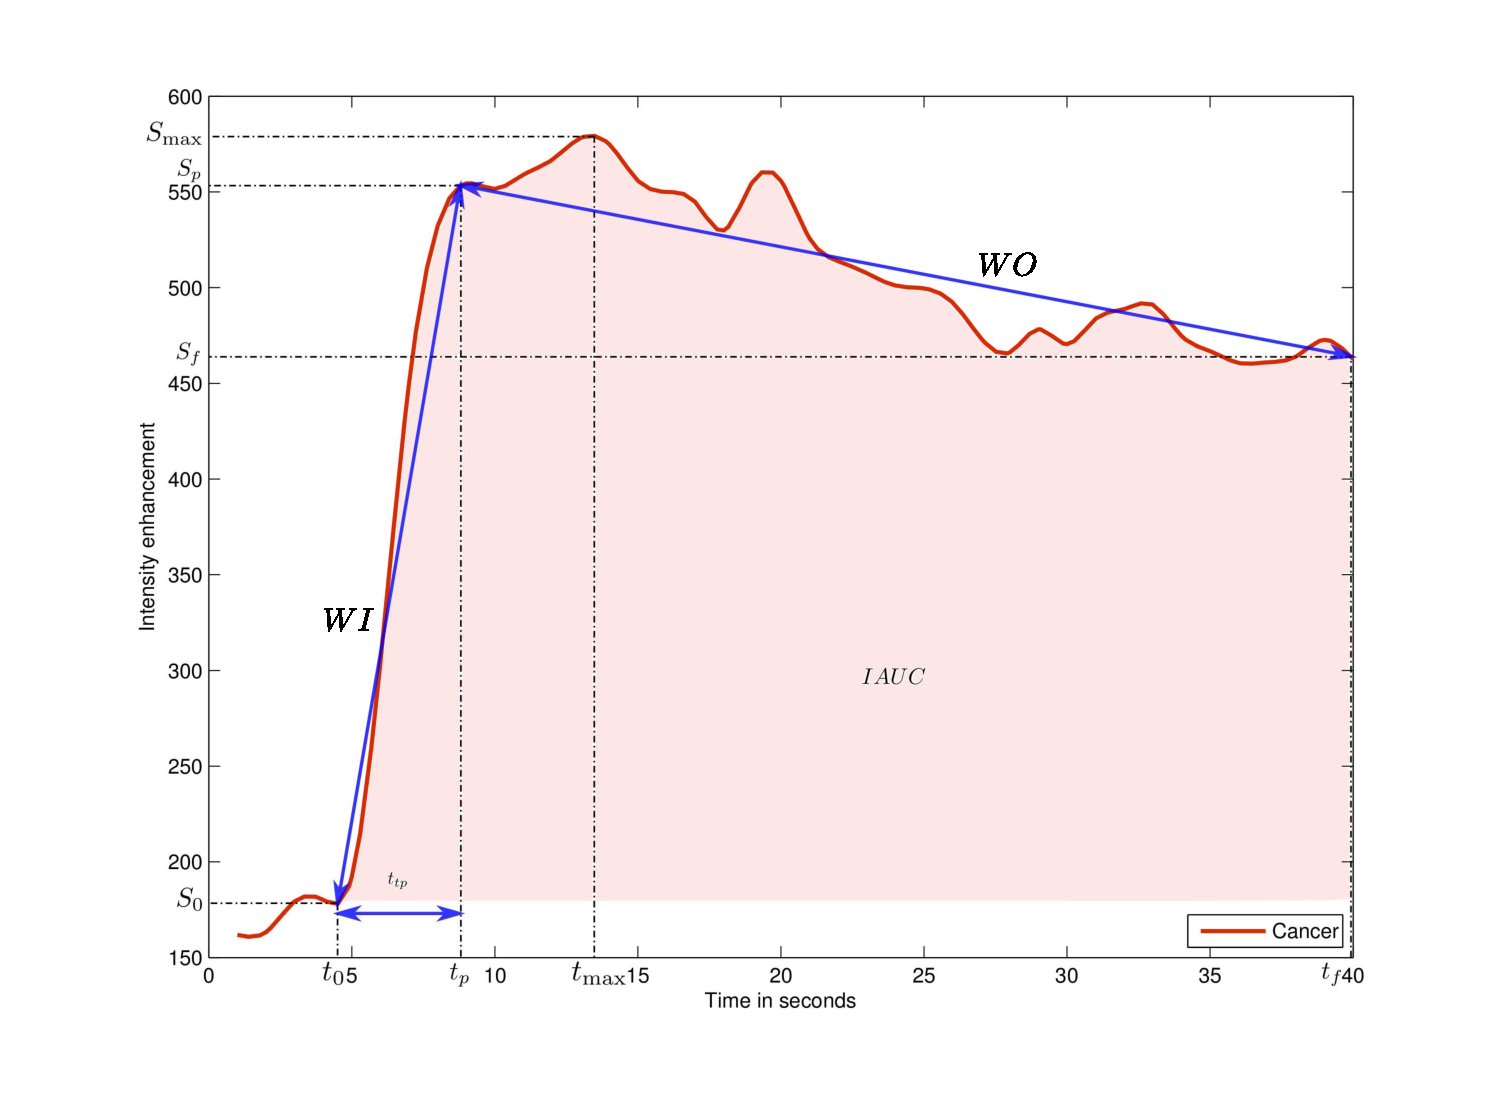
\includegraphics[width=.6\linewidth]{12_figures/figures/dce/dce_cancer_parameters.eps}
  \caption{Graphical representation of the different semi-quantitative features used for \ac{dce}-\ac{mri} analysis.}
  \label{fig:dceparam}
\end{figure}

\begin{figure}
  \centering
  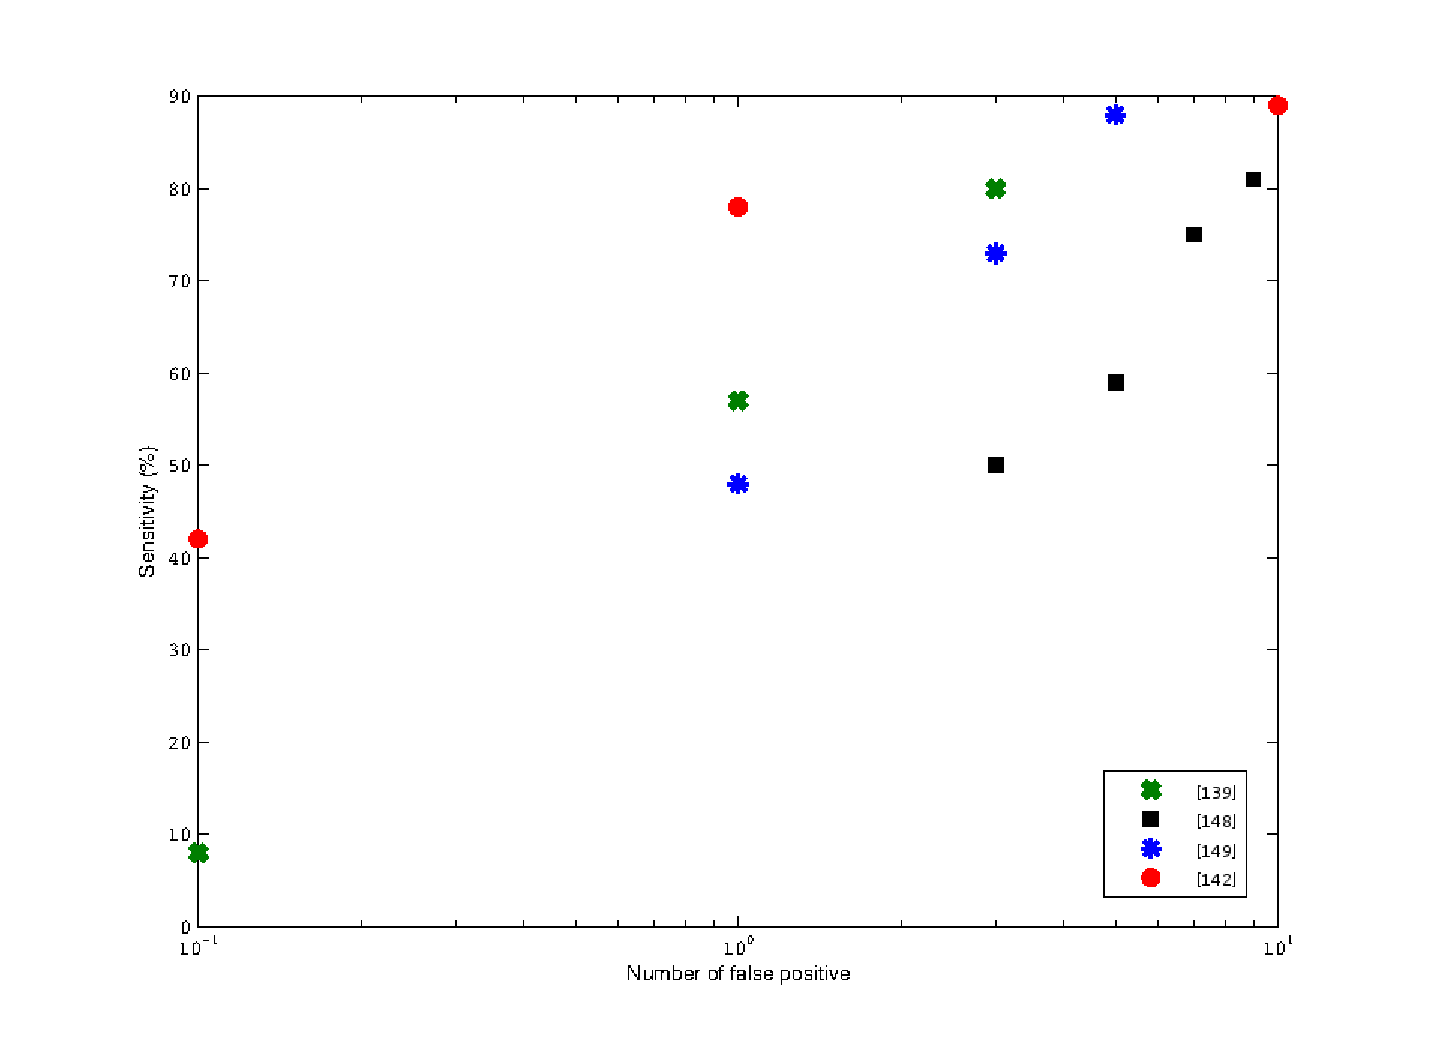
\includegraphics[width=.5\linewidth]{12_figures/figures/froc/froc.eps}
  \caption{Comparison in terms of \ac{froc} of the methods using data from 3.0 Tesla \ac{mri} scanner.}
  \label{fig:froc}
\end{figure}

\newgeometry{bottom=2.2cm,top=2.2cm}
\begin{figure*}
  \centering
  \hspace*{\fill}
  \subfigure[]{
    \label{fig:auc15}
    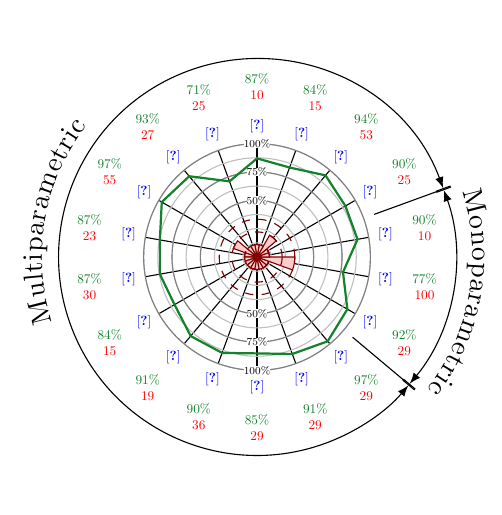
\begin{tikzpicture}[scale=.48,every node/.style={scale=0.48}]

      \def\labels{
        {\color{blue}\cite{Ampeliotis2008}},
        {\color{blue}\cite{Antic2013}},
        {\color{blue}\cite{Chan2003}},
        {\color{blue}\cite{Giannini2013}},
        {\color{blue}\cite{Langer2009}},
        {\color{blue}\cite{Lopes2011}},
        {\color{blue}\cite{Lv2009}},
        {\color{blue}\cite{Niaf2011}},
        {\color{blue}\cite{Niaf2012}},
        {\color{blue}\cite{Tiwari2009a}},
        {\color{blue}\cite{Tiwari2010}},
        {\color{blue}\cite{Tiwari2012}},
        {\color{blue}\cite{Tiwari2013}},
        {\color{blue}\cite{Vos2008}},
        {\color{blue}\cite{Vos2010}},
        {\color{blue}\cite{Mazzetti2011}},
        {\color{blue}\cite{Puech2009}},
        {\color{blue}\cite{Vos2008a}}
      }

      \def\reward{90,94,84,87,71,93,97,87,87,84,91,90,85,91,97,92,77,90}
      \def\dbSize{25,53,15,10,25,27,55,23,30,15,19,36,29,29,29,29,100,10}
      \def\dbClass{1,2,1,1,1,1,2,1,1,1,1,1,1,1,1,1,3,1}		
      \def\cZoom{3} 
      \def\percentageLabelAngle{90}
      \def\nbeams{18}
      \pgfmathsetmacro\beamAngle{(360/\nbeams)}
      \pgfmathsetmacro\halfAngle{(180/\nbeams)}
      \pgfmathsetmacro\globalRotation{\halfAngle}

      % draw the radiants
      \foreach \n  [count=\ni] in \labels
      {
        \pgfmathsetmacro\cAngle{{(\ni*(360/\nbeams))+\globalRotation}}
        \draw	(\cAngle:{\cZoom*1.15})  node[fill=white] {\n};
        \draw [thin] (0,0) -- (\cAngle:{\cZoom*1}) ;

      }

      % draw the % rings 
      \foreach \x in {12.5,25, ...,100} 
      \draw [thin,color=gray!50] (0,0) circle [radius={\cZoom*\x/100}];

      \foreach \x in {50,75,100}
      { 
        \draw [thin,color=black!50] (0,0) circle [radius={\cZoom/100*\x}];
        \foreach \a in {0, 180} \draw ({\percentageLabelAngle+\a}:{\cZoom*0.01*\x}) node  [inner sep=0pt,outer sep=0pt,fill=white,font=\fontsize{8}{8.5}\selectfont]{$\x\%$};
      }

      % draw the path of the percentages
      \def\aux{{\reward}}
      \pgfmathsetmacro\origin{\aux[\nbeams-1]} 
      \draw [semiAuto, thick] (\globalRotation:{\cZoom*\origin/100}) \foreach \n  [count=\ni] in \reward { -- ({(\ni*(360/\nbeams))+\globalRotation}:{\cZoom*\n/100}) } ;

      % label all the percentags
      \foreach \n [count=\ni] in \dbSize 
      {
	\pgfmathsetmacro\cAngle{{(\ni*(360/\nbeams))+\globalRotation}}
	\pgfmathsetmacro\nreward{\aux[\ni-1]}
	\draw (\cAngle:{\cZoom*1.5}) node[align=center] {{\color{semiAuto}\nreward $\%$} \\ {\color{red}\n} };
      } ;

      % draw the database rose
      \def\dbScale{\9}
      \foreach \n [count=\ni] in \dbClass
      \filldraw[fill=red!20!white, draw=red!50!black]
      (0,0) -- ({\ni*(360/\nbeams)-\halfAngle+\globalRotation}:{\cZoom*\n/9}) arc ({\ni*(360/\nbeams)-\halfAngle+\globalRotation}:{\ni*(360/\nbeams)+\halfAngle+\globalRotation}:{\cZoom*\n/9}) -- cycle;
      \foreach \x in {1,2,3}
      \draw [thin,color=red!50!black,dashed] (0,0) circle [radius={\cZoom*\x/9}];

      %% draw the domain of each class 
      \def\puta{	15/0/{Multiparametric},
        3/15/{Monoparametric}}

      \foreach \numElm/\contadorQueNoSeCalcular/\name [count=\ni] in \puta
      {

 	\pgfmathsetmacro\initialAngle{(\contadorQueNoSeCalcular*\beamAngle)+\halfAngle+\globalRotation}
 	\pgfmathsetmacro\finalAngle  {((\numElm+\contadorQueNoSeCalcular)*\beamAngle)+\halfAngle+\globalRotation}
	\pgfmathsetmacro\l  {\cZoom*1.65+.3pt}
	\draw (\initialAngle:{\cZoom*1.7}) -- (\initialAngle:{\cZoom*1.1});
	\draw [ |<->|,>=latex] (\initialAngle:\l) arc (\initialAngle:\finalAngle:\l) ;    									 
	\pgfmathsetmacro\r  {\cZoom*1.65+.45pt}
    	{\draw [decoration={raise=4pt,text along path,text={\name},text align={center}},decorate] (\finalAngle:\r) arc (\finalAngle:\initialAngle:\r);}
      }
      
    \end{tikzpicture}}\hfill
  \subfigure[]{
    \label{fig:auc30}
    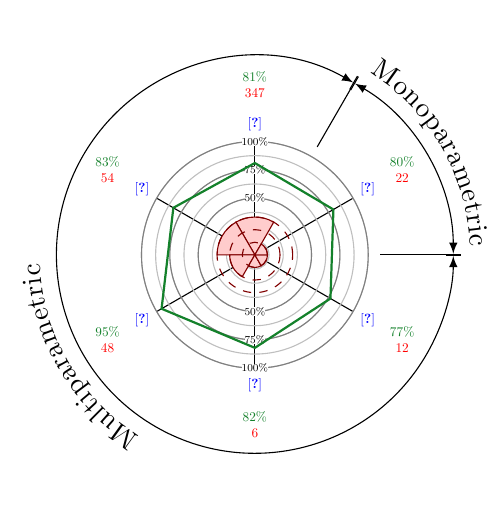
\begin{tikzpicture}[scale=.48,every node/.style={scale=0.48}]

      \def\labels{
        {\color{blue}\cite{Litjens2014}},
        {\color{blue}\cite{Liu2013}},
        {\color{blue}\cite{Peng2013}},
        {\color{blue}\cite{Viswanath2009}},
        {\color{blue}\cite{Viswanath2011}},
        {\color{blue}\cite{Viswanath2012}}
      }

      \def\reward{81,83,95,82,77,80}
      \def\dbSize{347,54,48,6,12,22}
      \def\dbClass{3,3,2,1,1,1}		
      \def\cZoom{3} 
      \def\percentageLabelAngle{90}
      \def\nbeams{6}
      \pgfmathsetmacro\beamAngle{(360/\nbeams)}
      \pgfmathsetmacro\halfAngle{(180/\nbeams)}
      \pgfmathsetmacro\globalRotation{\halfAngle}

      % draw the radiants
      \foreach \n  [count=\ni] in \labels
      {
        \pgfmathsetmacro\cAngle{{(\ni*(360/\nbeams))+\globalRotation}}
        \draw	(\cAngle:{\cZoom*1.15})  node[fill=white] {\n};
        \draw [thin] (0,0) -- (\cAngle:{\cZoom*1}) ;

      }

      % draw the % rings 
      \foreach \x in {12.5,25, ...,100} 
      \draw [thin,color=gray!50] (0,0) circle [radius={\cZoom*\x/100}];

      \foreach \x in {50,75,100}
      { 
        \draw [thin,color=black!50] (0,0) circle [radius={\cZoom/100*\x}];
        \foreach \a in {0, 180} \draw ({\percentageLabelAngle+\a}:{\cZoom*0.01*\x}) node  [inner sep=0pt,outer sep=0pt,fill=white,font=\fontsize{8}{8.5}\selectfont]{$\x\%$};
      }

      % draw the path of the percentages
      \def\aux{{\reward}}
      \pgfmathsetmacro\origin{\aux[\nbeams-1]} 
      \draw [semiAuto, thick] (\globalRotation:{\cZoom*\origin/100}) \foreach \n  [count=\ni] in \reward { -- ({(\ni*(360/\nbeams))+\globalRotation}:{\cZoom*\n/100}) } ;

      % label all the percentags
      \foreach \n [count=\ni] in \dbSize 
      {
	\pgfmathsetmacro\cAngle{{(\ni*(360/\nbeams))+\globalRotation}}
	\pgfmathsetmacro\nreward{\aux[\ni-1]}
	\draw (\cAngle:{\cZoom*1.5}) node[align=center] {{\color{semiAuto}\nreward $\%$} \\ {\color{red}\n} };
      } ;

      % draw the database rose
      \def\dbScale{\9}
      \foreach \n [count=\ni] in \dbClass
      \filldraw[fill=red!20!white, draw=red!50!black]
      (0,0) -- ({\ni*(360/\nbeams)-\halfAngle+\globalRotation}:{\cZoom*\n/9}) arc ({\ni*(360/\nbeams)-\halfAngle+\globalRotation}:{\ni*(360/\nbeams)+\halfAngle+\globalRotation}:{\cZoom*\n/9}) -- cycle;
      \foreach \x in {1,2,3}
      \draw [thin,color=red!50!black,dashed] (0,0) circle [radius={\cZoom*\x/9}];

      %% draw the domain of each class 
      \def\puta{	5/0/{Multiparametric},
        1/5/{Monoparametric}}

      \foreach \numElm/\contadorQueNoSeCalcular/\name [count=\ni] in \puta
      {

 	\pgfmathsetmacro\initialAngle{(\contadorQueNoSeCalcular*\beamAngle)+\halfAngle+\globalRotation}
 	\pgfmathsetmacro\finalAngle  {((\numElm+\contadorQueNoSeCalcular)*\beamAngle)+\halfAngle+\globalRotation}
	\pgfmathsetmacro\l  {\cZoom*1.65+.3pt}
	\draw (\initialAngle:{\cZoom*1.7}) -- (\initialAngle:{\cZoom*1.1});
	\draw [ |<->|,>=latex] (\initialAngle:\l) arc (\initialAngle:\finalAngle:\l) ;    									 
	\pgfmathsetmacro\r  {\cZoom*1.65+.45pt}
    	{\draw [decoration={raise=4pt,text along path,  text={\name},text align={center}},decorate] (\finalAngle:\r) arc (\finalAngle:\initialAngle:\r);}
      }
      
    \end{tikzpicture}
  }
  \hspace*{\fill}
  \caption{Numerical and graphical comparison of the results in terms of AUC for 1.5 and 3.0 Tesla \ac{mri} scanners. The {\color{semiAuto}green} value represents the metric and are graphically reported in the {\color{semiAuto}green} curve in the center of the figure. The {\color{red}red} value and areas correspond to the number of patients in the dataset. The numbers between brackets in {blue\color{blue}} correspond to the reference as reported in \acs{tab}~\ref{tab:sumpap}.}
  \label{fig:auc}
\end{figure*}

% ------------------------------------------------------------------------------------------------------------------------

\begin{figure*}%
  \centering
  \hspace*{\fill}
  \subfigure[]{
    \label{fig:sens15}
    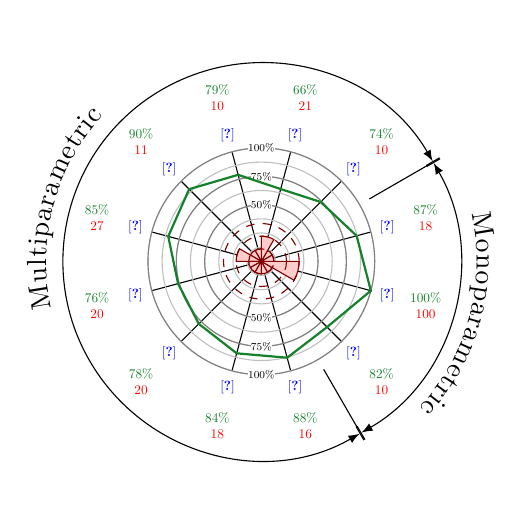
\begin{tikzpicture}[scale=.48,every node/.style={scale=0.48}]

      \def\labels{
        {\color{blue}\cite{Artan2009}},
        {\color{blue}\cite{Artan2010}},
        {\color{blue}\cite{Giannini2013}},
        {\color{blue}\cite{Liu2009}},
        {\color{blue}\cite{Lopes2011}},
        {\color{blue}\cite{Ozer2009}},
        {\color{blue}\cite{Ozer2010}},
        {\color{blue}\cite{Tiwari2009a}},
        {\color{blue}\cite{Viswanath2008}},
        {\color{blue}\cite{Mazzetti2011}},
        {\color{blue}\cite{Puech2009}},
        {\color{blue}\cite{Tiwari2008}}
      }

      \def\reward{74,66,79,90,85,76,78,84,88,82,100,87}
      \def\dbSize{10,21,10,11,27,20,20,18,16,10,100,18}
      \def\dbClass{1,2,1,1,2,1,1,1,1,1,3,1}		
      \def\cZoom{3} 
      \def\percentageLabelAngle{90}
      \def\nbeams{12}
      \pgfmathsetmacro\beamAngle{(360/\nbeams)}
      \pgfmathsetmacro\halfAngle{(180/\nbeams)}
      \pgfmathsetmacro\globalRotation{\halfAngle}

      % draw the radiants
      \foreach \n  [count=\ni] in \labels
      {
        \pgfmathsetmacro\cAngle{{(\ni*(360/\nbeams))+\globalRotation}}
        \draw	(\cAngle:{\cZoom*1.15})  node[fill=white] {\n};
        \draw [thin] (0,0) -- (\cAngle:{\cZoom*1}) ;

      }

      % draw the % rings 
      \foreach \x in {12.5,25, ...,100} 
      \draw [thin,color=gray!50] (0,0) circle [radius={\cZoom*\x/100}];

      \foreach \x in {50,75,100}
      { 
        \draw [thin,color=black!50] (0,0) circle [radius={\cZoom/100*\x}];
        \foreach \a in {0, 180} \draw ({\percentageLabelAngle+\a}:{\cZoom*0.01*\x}) node  [inner sep=0pt,outer sep=0pt,fill=white,font=\fontsize{8}{8.5}\selectfont]{$\x\%$};
      }

      % draw the path of the percentages
      \def\aux{{\reward}}
      \pgfmathsetmacro\origin{\aux[\nbeams-1]} 
      \draw [semiAuto, thick] (\globalRotation:{\cZoom*\origin/100}) \foreach \n  [count=\ni] in \reward { -- ({(\ni*(360/\nbeams))+\globalRotation}:{\cZoom*\n/100}) } ;

      % label all the percentags
      \foreach \n [count=\ni] in \dbSize 
      {
	\pgfmathsetmacro\cAngle{{(\ni*(360/\nbeams))+\globalRotation}}
	\pgfmathsetmacro\nreward{\aux[\ni-1]}
	\draw (\cAngle:{\cZoom*1.5}) node[align=center] {{\color{semiAuto}\nreward $\%$} \\ {\color{red}\n} };
      } ;

      % draw the database rose
      \def\dbScale{\9}
      \foreach \n [count=\ni] in \dbClass
      \filldraw[fill=red!20!white, draw=red!50!black]
      (0,0) -- ({\ni*(360/\nbeams)-\halfAngle+\globalRotation}:{\cZoom*\n/9}) arc ({\ni*(360/\nbeams)-\halfAngle+\globalRotation}:{\ni*(360/\nbeams)+\halfAngle+\globalRotation}:{\cZoom*\n/9}) -- cycle;
      \foreach \x in {1,2,3}
      \draw [thin,color=red!50!black,dashed] (0,0) circle [radius={\cZoom*\x/9}];

      %% draw the domain of each class 
      \def\puta{	9/0/{Multiparametric},
        3/9/{Monoparametric}}

      \foreach \numElm/\contadorQueNoSeCalcular/\name [count=\ni] in \puta
      {

 	\pgfmathsetmacro\initialAngle{(\contadorQueNoSeCalcular*\beamAngle)+\halfAngle+\globalRotation}
 	\pgfmathsetmacro\finalAngle  {((\numElm+\contadorQueNoSeCalcular)*\beamAngle)+\halfAngle+\globalRotation}
	\pgfmathsetmacro\l  {\cZoom*1.65+.3pt}
	\draw (\initialAngle:{\cZoom*1.7}) -- (\initialAngle:{\cZoom*1.1});
	\draw [ |<->|,>=latex] (\initialAngle:\l) arc (\initialAngle:\finalAngle:\l) ;    									 
	\pgfmathsetmacro\r  {\cZoom*1.65+.45pt}
    	{\draw [decoration={raise=4pt,text along path,  text={\name},text align={center}},decorate] (\finalAngle:\r) arc (\finalAngle:\initialAngle:\r);}
      }
      
    \end{tikzpicture}}\hfill
  \subfigure[]{
    \label{fig:spec15}
    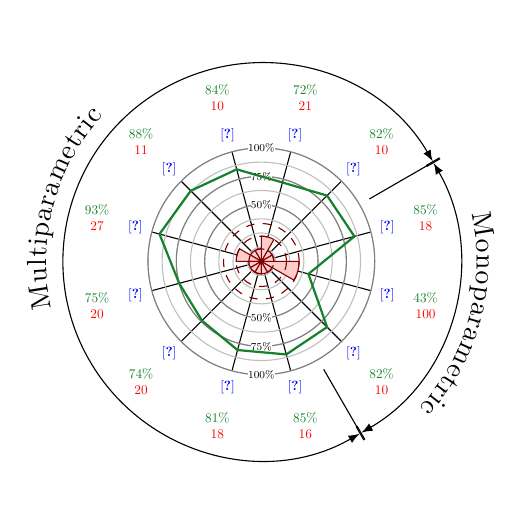
\begin{tikzpicture}[scale=.48,every node/.style={scale=0.48}]

      \def\labels{
        {\color{blue}\cite{Artan2009}},
        {\color{blue}\cite{Artan2010}},
        {\color{blue}\cite{Giannini2013}},
        {\color{blue}\cite{Liu2009}},
        {\color{blue}\cite{Lopes2011}},
        {\color{blue}\cite{Ozer2009}},
        {\color{blue}\cite{Ozer2010}},
        {\color{blue}\cite{Tiwari2009a}},
        {\color{blue}\cite{Viswanath2008}},
        {\color{blue}\cite{Mazzetti2011}},
        {\color{blue}\cite{Puech2009}},
        {\color{blue}\cite{Tiwari2008}}
      }

      \def\reward{82,72,84,88,93,75,74,81,85,82,43,85}
      \def\dbSize{10,21,10,11,27,20,20,18,16,10,100,18}
      \def\dbClass{1,2,1,1,2,1,1,1,1,1,3,1}		
      \def\cZoom{3} 
      \def\percentageLabelAngle{90}
      \def\nbeams{12}
      \pgfmathsetmacro\beamAngle{(360/\nbeams)}
      \pgfmathsetmacro\halfAngle{(180/\nbeams)}
      \pgfmathsetmacro\globalRotation{\halfAngle}

      % draw the radiants
      \foreach \n  [count=\ni] in \labels
      {
        \pgfmathsetmacro\cAngle{{(\ni*(360/\nbeams))+\globalRotation}}
        \draw	(\cAngle:{\cZoom*1.15})  node[fill=white] {\n};
        \draw [thin] (0,0) -- (\cAngle:{\cZoom*1}) ;

      }

      % draw the % rings 
      \foreach \x in {12.5,25, ...,100} 
      \draw [thin,color=gray!50] (0,0) circle [radius={\cZoom*\x/100}];

      \foreach \x in {50,75,100}
      { 
        \draw [thin,color=black!50] (0,0) circle [radius={\cZoom/100*\x}];
        \foreach \a in {0, 180} \draw ({\percentageLabelAngle+\a}:{\cZoom*0.01*\x}) node  [inner sep=0pt,outer sep=0pt,fill=white,font=\fontsize{8}{8.5}\selectfont]{$\x\%$};
      }

      % draw the path of the percentages
      \def\aux{{\reward}}
      \pgfmathsetmacro\origin{\aux[\nbeams-1]} 
      \draw [semiAuto, thick] (\globalRotation:{\cZoom*\origin/100}) \foreach \n  [count=\ni] in \reward { -- ({(\ni*(360/\nbeams))+\globalRotation}:{\cZoom*\n/100}) } ;

      % label all the percentags
      \foreach \n [count=\ni] in \dbSize 
      {
	\pgfmathsetmacro\cAngle{{(\ni*(360/\nbeams))+\globalRotation}}
	\pgfmathsetmacro\nreward{\aux[\ni-1]}
	\draw (\cAngle:{\cZoom*1.5}) node[align=center] {{\color{semiAuto}\nreward $\%$} \\ {\color{red}\n} };
      } ;

      % draw the database rose
      \def\dbScale{\9}
      \foreach \n [count=\ni] in \dbClass
      \filldraw[fill=red!20!white, draw=red!50!black]
      (0,0) -- ({\ni*(360/\nbeams)-\halfAngle+\globalRotation}:{\cZoom*\n/9}) arc ({\ni*(360/\nbeams)-\halfAngle+\globalRotation}:{\ni*(360/\nbeams)+\halfAngle+\globalRotation}:{\cZoom*\n/9}) -- cycle;
      \foreach \x in {1,2,3}
      \draw [thin,color=red!50!black,dashed] (0,0) circle [radius={\cZoom*\x/9}];

      %% draw the domain of each class 
      \def\puta{	9/0/{Multiparametric},
        3/9/{Monoparametric}}

      \foreach \numElm/\contadorQueNoSeCalcular/\name [count=\ni] in \puta
      {

 	\pgfmathsetmacro\initialAngle{(\contadorQueNoSeCalcular*\beamAngle)+\halfAngle+\globalRotation}
 	\pgfmathsetmacro\finalAngle  {((\numElm+\contadorQueNoSeCalcular)*\beamAngle)+\halfAngle+\globalRotation}
	\pgfmathsetmacro\l  {\cZoom*1.65+.3pt}
	\draw (\initialAngle:{\cZoom*1.7}) -- (\initialAngle:{\cZoom*1.1});
	\draw [ |<->|,>=latex] (\initialAngle:\l) arc (\initialAngle:\finalAngle:\l) ;    									 
	\pgfmathsetmacro\r  {\cZoom*1.65+.45pt}
    	{\draw [decoration={raise=4pt,text along path,  text={\name},text align={center}},decorate] (\finalAngle:\r) arc (\finalAngle:\initialAngle:\r);}
      }
      
    \end{tikzpicture}
  }
  \hspace*{\fill}
  \\
  \hspace*{\fill}
  \subfigure[]{
    \label{fig:sens30}
    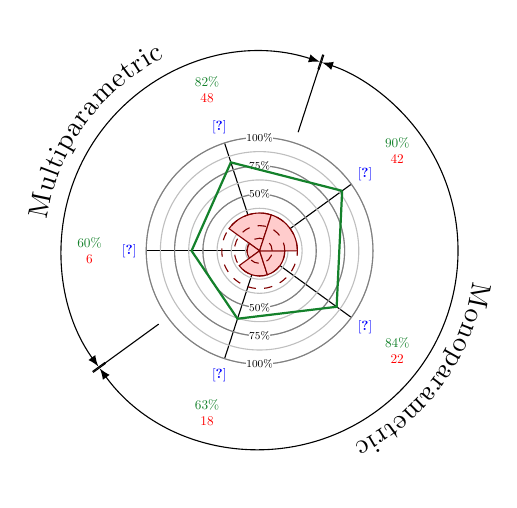
\begin{tikzpicture}[scale=.48,every node/.style={scale=0.48}]

      \def\labels{
        {\color{blue}\cite{Peng2013}},
        {\color{blue}\cite{Viswanath2008a}},
        {\color{blue}\cite{Matulewicz2013}},
        {\color{blue}\cite{Parfait2012}},
        {\color{blue}\cite{Sung2011}}
      }

      \def\reward{82,60,63,84,90}
      \def\dbSize{48,6,18,22,42}
      \def\dbClass{3,1,2,2,3}		
      \def\cZoom{3} 
      \def\percentageLabelAngle{90}
      \def\nbeams{5}
      \pgfmathsetmacro\beamAngle{(360/\nbeams)}
      \pgfmathsetmacro\halfAngle{(180/\nbeams)}
      \pgfmathsetmacro\globalRotation{\halfAngle}


      % draw the radiants
      \foreach \n  [count=\ni] in \labels
      {
        \pgfmathsetmacro\cAngle{{(\ni*(360/\nbeams))+\globalRotation}}
        \draw	(\cAngle:{\cZoom*1.15})  node[fill=white] {\n};
        \draw [thin] (0,0) -- (\cAngle:{\cZoom*1}) ;

      }

      % draw the % rings 
      \foreach \x in {12.5,25, ...,100} 
      \draw [thin,color=gray!50] (0,0) circle [radius={\cZoom*\x/100}];

      \foreach \x in {50,75,100}
      { 
        \draw [thin,color=black!50] (0,0) circle [radius={\cZoom/100*\x}];
        \foreach \a in {0, 180} \draw ({\percentageLabelAngle+\a}:{\cZoom*0.01*\x}) node  [inner sep=0pt,outer sep=0pt,fill=white,font=\fontsize{8}{8.5}\selectfont]{$\x\%$};
      }

      % draw the path of the percentages
      \def\aux{{\reward}}
      \pgfmathsetmacro\origin{\aux[\nbeams-1]} 
      \draw [semiAuto, thick] (\globalRotation:{\cZoom*\origin/100}) \foreach \n  [count=\ni] in \reward { -- ({(\ni*(360/\nbeams))+\globalRotation}:{\cZoom*\n/100}) } ;

      % label all the percentags
      \foreach \n [count=\ni] in \dbSize 
      {
	\pgfmathsetmacro\cAngle{{(\ni*(360/\nbeams))+\globalRotation}}
	\pgfmathsetmacro\nreward{\aux[\ni-1]}
	\draw (\cAngle:{\cZoom*1.5}) node[align=center] {{\color{semiAuto}\nreward $\%$} \\ {\color{red}\n} };
      } ;

      % draw the database rose
      \def\dbScale{\9}
      \foreach \n [count=\ni] in \dbClass
      \filldraw[fill=red!20!white, draw=red!50!black]
      (0,0) -- ({\ni*(360/\nbeams)-\halfAngle+\globalRotation}:{\cZoom*\n/9}) arc ({\ni*(360/\nbeams)-\halfAngle+\globalRotation}:{\ni*(360/\nbeams)+\halfAngle+\globalRotation}:{\cZoom*\n/9}) -- cycle;
      \foreach \x in {1,2,3}
      \draw [thin,color=red!50!black,dashed] (0,0) circle [radius={\cZoom*\x/9}];

      %% draw the domain of each class 
      \def\puta{	2/0/{Multiparametric},
        3/2/{Monoparametric}}

      \foreach \numElm/\contadorQueNoSeCalcular/\name [count=\ni] in \puta
      {

 	\pgfmathsetmacro\initialAngle{(\contadorQueNoSeCalcular*\beamAngle)+\halfAngle+\globalRotation}
 	\pgfmathsetmacro\finalAngle  {((\numElm+\contadorQueNoSeCalcular)*\beamAngle)+\halfAngle+\globalRotation}
	\pgfmathsetmacro\l  {\cZoom*1.65+.3pt}
	\draw (\initialAngle:{\cZoom*1.7}) -- (\initialAngle:{\cZoom*1.1});
	\draw [ |<->|,>=latex] (\initialAngle:\l) arc (\initialAngle:\finalAngle:\l) ;    									 
	\pgfmathsetmacro\r  {\cZoom*1.65+.45pt}
    	{\draw [decoration={raise=4pt,text along path,  text={\name},text align={center}},decorate] (\finalAngle:\r) arc (\finalAngle:\initialAngle:\r);}
      }
      
    \end{tikzpicture}}\hfill
  \subfigure[]{
    \label{fig:spec30}
    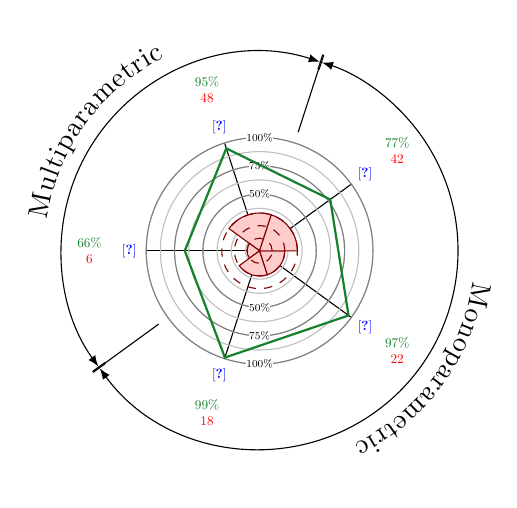
\begin{tikzpicture}[scale=.48,every node/.style={scale=0.48}]

      \def\labels{
        {\color{blue}\cite{Peng2013}},
        {\color{blue}\cite{Viswanath2008a}},
        {\color{blue}\cite{Matulewicz2013}},
        {\color{blue}\cite{Parfait2012}},
        {\color{blue}\cite{Sung2011}}
      }

      \def\reward{95,66,99,97,77}
      \def\dbSize{48,6,18,22,42}
      \def\dbClass{3,1,2,2,3}		
      \def\cZoom{3} 
      \def\percentageLabelAngle{90}
      \def\nbeams{5}
      \pgfmathsetmacro\beamAngle{(360/\nbeams)}
      \pgfmathsetmacro\halfAngle{(180/\nbeams)}
      \pgfmathsetmacro\globalRotation{\halfAngle}

      % draw the radiants
      \foreach \n  [count=\ni] in \labels
      {
        \pgfmathsetmacro\cAngle{{(\ni*(360/\nbeams))+\globalRotation}}
        \draw	(\cAngle:{\cZoom*1.15})  node[fill=white] {\n};
        \draw [thin] (0,0) -- (\cAngle:{\cZoom*1}) ;

      }

      % draw the % rings 
      \foreach \x in {12.5,25, ...,100} 
      \draw [thin,color=gray!50] (0,0) circle [radius={\cZoom*\x/100}];

      \foreach \x in {50,75,100}
      { 
        \draw [thin,color=black!50] (0,0) circle [radius={\cZoom/100*\x}];
        \foreach \a in {0, 180} \draw ({\percentageLabelAngle+\a}:{\cZoom*0.01*\x}) node  [inner sep=0pt,outer sep=0pt,fill=white,font=\fontsize{8}{8.5}\selectfont]{$\x\%$};
      }

      % draw the path of the percentages
      \def\aux{{\reward}}
      \pgfmathsetmacro\origin{\aux[\nbeams-1]} 
      \draw [semiAuto, thick] (\globalRotation:{\cZoom*\origin/100}) \foreach \n  [count=\ni] in \reward { -- ({(\ni*(360/\nbeams))+\globalRotation}:{\cZoom*\n/100}) } ;

      % label all the percentags
      \foreach \n [count=\ni] in \dbSize 
      {
	\pgfmathsetmacro\cAngle{{(\ni*(360/\nbeams))+\globalRotation}}
	\pgfmathsetmacro\nreward{\aux[\ni-1]}
	\draw (\cAngle:{\cZoom*1.5}) node[align=center] {{\color{semiAuto}\nreward $\%$} \\ {\color{red}\n} };
      } ;

      % draw the database rose
      \def\dbScale{\9}
      \foreach \n [count=\ni] in \dbClass
      \filldraw[fill=red!20!white, draw=red!50!black]
      (0,0) -- ({\ni*(360/\nbeams)-\halfAngle+\globalRotation}:{\cZoom*\n/9}) arc ({\ni*(360/\nbeams)-\halfAngle+\globalRotation}:{\ni*(360/\nbeams)+\halfAngle+\globalRotation}:{\cZoom*\n/9}) -- cycle;
      \foreach \x in {1,2,3}
      \draw [thin,color=red!50!black,dashed] (0,0) circle [radius={\cZoom*\x/9}];

      %% draw the domain of each class 
      \def\puta{	2/0/{Multiparametric},
        3/2/{Monoparametric}}

      \foreach \numElm/\contadorQueNoSeCalcular/\name [count=\ni] in \puta
      {

 	\pgfmathsetmacro\initialAngle{(\contadorQueNoSeCalcular*\beamAngle)+\halfAngle+\globalRotation}
 	\pgfmathsetmacro\finalAngle  {((\numElm+\contadorQueNoSeCalcular)*\beamAngle)+\halfAngle+\globalRotation}
	\pgfmathsetmacro\l  {\cZoom*1.65+.3pt}
	\draw (\initialAngle:{\cZoom*1.7}) -- (\initialAngle:{\cZoom*1.1});
	\draw [ |<->|,>=latex] (\initialAngle:\l) arc (\initialAngle:\finalAngle:\l) ;    									 
	\pgfmathsetmacro\r  {\cZoom*1.65+.45pt}
    	{\draw [decoration={raise=4pt,text along path,  text={\name},text align={center}},decorate] (\finalAngle:\r) arc (\finalAngle:\initialAngle:\r);}
      }
      
    \end{tikzpicture}
  }
  \hspace*{\fill}
  \caption{Numerical and graphical comparison of the results in terms of sensitivity~\subref{fig:sens15},~\subref{fig:sens30} and specificity~\subref{fig:spec15},~\subref{fig:spec30} for 1.5 and 3.0 Tesla \ac{mri} scanners. The value in {\color{semiAuto}green} represents the metric and are graphically reported in the {\color{semiAuto}green} curve in the center of the figure. The {\color{red}red} value and areas correspond to the number of patients in the dataset. The numbers between brackets in {\color{blue}blue} correspond to the reference as reported in \acs{tab}~\ref{tab:sumpap}.}
  \label{fig:sensspec}
\end{figure*}
\restoregeometry

%%% Local Variables: 
%%% mode: latex
%%% TeX-master: "../g_lemaitre_state_of_the_art"
%%% End: 



\begin{table*}
\begin{adjustwidth}{-1cm}{}
\caption{Overview of the features associated with each \ac{mri} modality used for medical diagnosis by radiologists. Acronyms: \acf{cap} - \acf{si} - \acf{gs}.}	
\begin{threeparttable}
\centering
\small
\renewcommand{\arraystretch}{1.2}
	\begin{tabular}{|m{1.7cm}||m{4.5cm}|>{\centering\arraybackslash}m{3.5cm}|>{\centering\arraybackslash}m{4cm}|>{\centering\arraybackslash}m{2cm}|}\hline
	\rowcolor{gray!10}
	Modality & Significant features & \ac{cap} & Healthy tissue & \ac{gs} correlation \\ \hline \hline
	\ac{t2w} \ac{mri} & \acs{si} & low-\ac{si} & intermediate to high-\ac{si} & + \\ \hline
	T$_2$ map & \acs{si} & low-\ac{si} & intermediate to high-\ac{si} & + \\ \hline
	\multirow{9}{*}{\ac{dce} \ac{mri}} & Semi-quantitative features: & & & \\[-1.5ex]
	& $-$ wash-in & faster & slower & 0 \\[-1.5ex]
	& $-$ wash-out & faster & slower & 0 \\[-1.5ex]
	& $-$ integral under the curve & higher & lower & 0 \\[-1.5ex]
	& $-$ maximum signal intensity & higher & lower & 0 \\[-1.5ex]
	& $-$ time-to-peak enhancement & faster & slower & 0 \\ \cline{2-5}
	& Quantitative features (Tofts' parameters): & & & \\[-1.5ex]
	& $-$ $\text{k}_{\text{ep}}$ & higher & lower & 0 \\[-1.5ex]
	& $-$ $\text{K}^{\text{trans}}$ & higher & lower & 0 \\ \hline
	\ac{dw} \ac{mri} & \acs{si} & higher-\ac{si} & lower-\ac{si} & + \\ \hline
	\acs{adc} map & \acs{si} & low-\ac{si} & high-\ac{si} & + \\ \hline
	\multirow{4}{*}{\ac{mrsi}}& Metabolites: & & & \\[-1.5ex]
	& Citrate (2.64 ppm) & lower concentration & higher concentration & + \\[-1.5ex]
	& Choline (3.21 ppm) & higher concentration & lower concentration & 0 \\[-1.5ex]
	& Spermine (3.11 ppm) & lower concentration & higher concentration & + \\ \hline
	
	\end{tabular}
	\begin{tablenotes}
      \small
      \item Notes:
      \item + = significantly correlated.
      \item 0 = no correlation.
    \end{tablenotes}
\end{threeparttable}
\end{adjustwidth}
\label{tab:modmri}
\end{table*}

\newgeometry{margin=.5cm}
\thispagestyle{empty}
\begin{table*}
\centering
\caption{Overview of the different studies reviewed with their main characteristics. Acronyms: number (\#) - image regularization (Img. Reg.).}
\scriptsize
%\begin{adjustwidth}{-2.2cm}{}
\begin{threeparttable}
\renewcommand{\arraystretch}{1}	
	\rowcolors{3}{black!5}{white}	
	\begin{tabular}{|>{\centering\arraybackslash}m{0.7cm}|>{\centering\arraybackslash}m{3cm}|>{\centering\arraybackslash}m{0.8cm}|>{\centering\arraybackslash}m{0.8cm}>{\centering\arraybackslash}m{0.8cm}>{\centering\arraybackslash}m{1cm}>{\centering\arraybackslash}m{1cm}|>{\centering\arraybackslash}m{0.7cm}>{\centering\arraybackslash}m{0.7cm}|>{\centering\arraybackslash}m{0.7cm}>{\centering\arraybackslash}m{0.7cm}|>{\centering\arraybackslash}m{0.7cm}>{\centering\arraybackslash}m{0.7cm}>{\centering\arraybackslash}m{0.7cm}|}\hline
	\hiderowcolors
	\multirow{2}{*}{Index} & \multirow{2}{*}{Study} & \# & \multicolumn{4}{c|}{\ac{mri}-modality} & \multicolumn{2}{c|}{Strength of field} & \multicolumn{2}{c|}{Studied zones} & \multicolumn{3}{c|}{\ac{cad} stages} \\ \cline{4-14}
	 & & patients & \ac{t2w} \ac{mri} & \ac{dce} \ac{mri} & \ac{dw} \ac{mri} & \ac{mrsi} & 1.5 T & 3.0 T & \ac{pz} & \ac{cg} & Img. Reg. & \ac{cade} & \ac{cadx} \\ \hline \hline
	 \showrowcolors 
	 	 \cite{Ampeliotis2007} & Ampeliotis et al.\,(2007) & 25 & \cmark & \cmark & \xmark & \xmark & \cmark & \xmark & \cmark & \xmark & \mmark & \xmark & \cmark \\
	 	 \cite{Ampeliotis2008} & Ampeliotis et al.\,(2008) & 25 & \cmark & \cmark & \xmark & \xmark & \cmark & \xmark & \cmark & \xmark & \mmark & \xmark & \cmark \\
	 	 \cite{Antic2013} & Antic et al.\,(2013) & 53 & \cmark & \xmark & \cmark & \xmark & \cmark & \xmark & \cmark & \cmark & \xmark  & \xmark & \cmark \\
	 	 \cite{Artan2009} & Artan et al.\,(2009) & 10 & \cmark & \cmark & \cmark & \xmark & \cmark & \xmark & \cmark & \xmark  & \xmark & \cmark & \cmark \\
	 	 \cite{Artan2010} & Artan et al.\,(2010) & 21 & \cmark & \cmark & \cmark & \xmark & \cmark & \xmark & \cmark & \xmark & \mmark & \cmark & \cmark \\
	 	 \cite{Chan2003} & Chan et al.\,(2013) & 15 & \cmark & \xmark & \cmark & \xmark & \cmark & \xmark & \cmark & \xmark & \xmark & \xmark & \cmark \\
	 	 \cite{Giannini2013} & Giannini et al.\,(2013) & 10 & \cmark & \cmark & \cmark & \xmark & \cmark & \xmark & \cmark & \xmark & \cmark & \cmark & \cmark \\
	 	 \cite{Kelm2007} & Kelm et al.\,(2007) & 24 & \xmark & \xmark & \xmark & \cmark & \cmark & \xmark & \cmark & \cmark & \mmark & \cmark & \cmark \\
	 	 \cite{Langer2009} & Langer et al.\,(2009) & 25 & \cmark & \cmark & \cmark & \xmark & \cmark & \xmark & \cmark & \xmark & \mmark & \xmark & \cmark \\
	 	 \cite{Litjens2011} & Litjens et al.\,(2011) & 188 & \cmark & \cmark & \cmark & \xmark & \xmark & \cmark & \cmark & \xmark & \mmark & \cmark & \cmark \\
	 	 \cite{Litjens2012} & Litjens et al.\,(2012) & 288 & \cmark & \cmark & \cmark & \xmark & \xmark & \cmark & \cmark & \cmark & \mmark & \cmark & \cmark \\
	 	 \cite{Litjens2014} & Litjens et al.\,(2014) & 347 & \cmark & \cmark & \cmark & \xmark & \xmark & \cmark & \cmark & \cmark & \mmark & \cmark & \cmark \\
	 	 \cite{Liu2009} & Liu et al.\,(2009) & 11 & \cmark & \cmark & \cmark & \xmark & \cmark & \xmark & \cmark & \xmark & \mmark & \cmark & \cmark \\
	 	 \cite{Liu2013} & Liu et al.\,(2013) & 54 & \cmark & \cmark & \cmark & \xmark & \xmark & \cmark & \cmark & \cmark & \mmark & \xmark & \cmark \\
	 	 \cite{Lopes2011} & Lopes et al.\,(2011) & 27 & \cmark & \xmark & \xmark & \xmark & \cmark & \xmark & \cmark & \xmark & \mmark & \cmark & \cmark \\
	 	 \cite{Lv2009} & Lv et al.\,(2009) & 55 & \cmark & \xmark & \xmark & \xmark & \cmark & \xmark & \cmark & \xmark & \mmark & \xmark & \cmark \\
	 	 \cite{Matulewicz2013} & Matulewicz et al.\,(2013) & 18 & \xmark & \xmark & \xmark & \cmark & \xmark & \cmark & \cmark & \cmark & \xmark & \cmark & \cmark \\ 
	 	 \cite{Mazzetti2011} & Mazzetti et al.\,(2011) & 10 & \xmark & \cmark & \xmark & \xmark & \cmark & \xmark & \cmark & \xmark & \mmark & \cmark & \cmark \\
	 	 \cite{Niaf2011} & Niaf et al.\,(2011) & 23 & \cmark & \cmark & \cmark & \xmark & \cmark & \xmark & \cmark & \xmark & \mmark & \xmark & \cmark \\
	 	 \cite{Niaf2012} & Niaf et al.\,(2012) & 30 & \cmark & \cmark & \cmark & \xmark & \cmark & \xmark & \cmark & \xmark & \mmark & \xmark & \cmark \\
	 	 \cite{Ozer2009} & Ozer et al.\,(2009) & 20 & \cmark & \cmark & \cmark & \xmark & \cmark & \xmark & \cmark & \xmark & \mmark & \cmark & \cmark \\
	 	 \cite{Ozer2010} & Ozer et al.\,(2010) & 20 & \cmark & \cmark & \cmark & \xmark & \cmark & \xmark & \cmark & \xmark & \mmark & \cmark & \cmark \\
	 	 \cite{Parfait2012} & Parfait et al.\,(2012) & 22 & \xmark & \xmark & \xmark & \cmark & \xmark & \cmark & \cmark & \cmark & \mmark & \cmark & \cmark \\
	 	 \cite{Peng2013} & Peng et al.\,(2013) & 48 & \cmark & \cmark & \cmark & \xmark & \xmark & \cmark & \cmark & \cmark & \xmark & \xmark & \cmark \\
	 	 \cite{Puech2009} & Puech et al.\,(2009) & 100 & \xmark & \cmark & \xmark & \xmark & \cmark & \xmark & \cmark & \cmark & \xmark & \xmark & \cmark \\
	 	 \cite{Sung2011} & Sung et al.\,(2011) & 42 & \xmark & \cmark & \xmark & \xmark & \xmark & \cmark & \cmark & \cmark & \xmark & \cmark & \cmark \\
	 	 \cite{Tiwari2007} & Tiwari et al.\,(2007) & 14 & \xmark & \xmark & \xmark & \cmark & \cmark & \xmark & \cmark & \cmark & \mmark & \cmark & \cmark \\
	 	 \cite{Tiwari2008} & Tiwari et al.\,(2008) & 18 & \xmark & \xmark & \xmark & \cmark & \cmark & \xmark & \cmark & \cmark & \mmark & \cmark & \cmark \\
	 	 \cite{Tiwari2009} & Tiwari et al.\,(2009) & 18 & \xmark & \xmark & \xmark & \cmark & \cmark & \xmark & \cmark & \cmark & \mmark & \cmark & \cmark \\
	 	 \cite{Tiwari2009a} & Tiwari et al.\,(2009) & 15 & \cmark & \xmark & \xmark & \cmark & \cmark & \xmark & \cmark & \cmark & \mmark & \cmark & \cmark \\
	 	 \cite{Tiwari2010} & Tiwari et al.\,(2010) & 19 & \cmark & \xmark & \xmark & \cmark & \cmark & \xmark & \cmark & \cmark & \mmark & \cmark & \cmark \\
	 	 \cite{Tiwari2012} & Tiwari et al.\,(2012) & 36 & \cmark & \xmark & \xmark & \cmark & \cmark & \xmark & \cmark & \cmark & \xmark & \cmark & \cmark \\
	 	 \cite{Tiwari2013} & Tiwari et al.\,(2013) & 29 & \cmark & \xmark & \xmark & \cmark & \cmark & \xmark & \cmark & \cmark & \mmark & \cmark & \cmark \\
	 	 \cite{Viswanath2008} & Viswanath et al.\,(2008) & 16 & \cmark & \xmark & \xmark & \cmark & \cmark & \xmark & \cmark & \cmark & \xmark & \cmark & \cmark \\
	 	 \cite{Viswanath2008a} & Viswanath et al.\,(2008) & 6 & \cmark & \cmark & \xmark & \xmark & \xmark & \cmark & \cmark & \cmark & \mmark & \cmark & \cmark \\
	 	 \cite{Viswanath2009} & Viswanath et al.\,(2009) & 6 & \cmark & \cmark & \xmark & \xmark & \xmark & \cmark & \cmark & \cmark & \cmark & \cmark & \cmark \\
	 	 \cite{Viswanath2011} & Viswanath et al.\,(2011) & 12 & \cmark & \cmark & \cmark & \xmark & \xmark & \cmark & \cmark & \cmark & \mmark & \cmark & \cmark \\
	 	 \cite{Viswanath2012} & Viswanath et al.\,(20012) & 22 & \cmark & \xmark & \xmark & \xmark & \xmark & \cmark & \cmark & \cmark & \cmark & \cmark & \cmark \\
	 	 \cite{Vos2008} & Vos et al.\,(2008) & 29 & \cmark & \cmark & \xmark & \xmark & \cmark & \xmark & \cmark & \xmark & \mmark & \xmark & \cmark \\
	 	 \cite{Vos2008a} & Vos et al.\,(2008) & 29 & \xmark & \cmark & \xmark & \xmark & \cmark & \xmark & \cmark & \xmark & \mmark & \xmark & \cmark \\
	 	 \cite{Vos2010} & Vos et al.\,(2010) & 29 & \cmark & \cmark & \xmark & \xmark & \cmark & \xmark & \cmark & \xmark & \mmark & \xmark & \cmark \\
	 	 \cite{Vos2012} & Vos et al.\,(2012) & NA & \cmark & \cmark & \cmark & \xmark & \xmark & \cmark & \cmark & \xmark & \mmark & \cmark & \cmark \\
	 	 \hline
	\end{tabular}
	\begin{tablenotes}
      \footnotesize
      \item Notes:
      \item {\xmark}: not used or not implemented.
      \item {\mmark}: partially implemented.
      \item {\cmark}: used or implemented.
    \end{tablenotes}
\end{threeparttable}
%\end{adjustwidth}
\label{tab:sumpap}
\end{table*}
\restoregeometry

\begin{table}
	\caption{Overview of the pre-processing methods used in \ac{cad} systems.}
	\small
	\renewcommand{\arraystretch}{1}
	\begin{tabular}{p{.65\linewidth} p{.25\linewidth}}
		\hline \\ [-1.5ex]
		\textbf{Pre-processing operations} & \textbf{References} \\ \\ [-1.5ex]
		\hline \\ [-1.5ex]
		\textit{\ac{mri} pre-processing:} & \\ \\ [-1.5ex]
		\quad Noise filtering: &  \\
		\quad \quad Median filtering & \cite{Ozer2009,Ozer2010}  \\
		\quad \quad Wavelet-based filtering & \cite{Ampeliotis2007,Ampeliotis2008,Lopes2011} \\ \\ [-1.5ex]
		\quad Bias correction: & \\
		\quad \quad Parametric methods & \cite{Lv2009,Viswanath2009} \\
		\quad \quad Non-parametric methods & \cite{Viswanath2011} \\ \\ [-1.5ex]
		\quad Standardization: & \\
		\quad \quad Statistical-based normalization: & \cite{Artan2009,Artan2010,Lv2009,Ozer2009,Ozer2010,Viswanath2009,Viswanath2011,Viswanath2012} \\
		\quad \quad Organ \ac{si}-based normalization & \cite{Niaf2011,Niaf2012} \\ \\ [-1.5ex]
		\textit{\ac{mrsi} pre-processing:} & \\ \\ [-1.5ex]
		\quad Phase correction & \cite{Parfait2012} \\
		\quad Water and lipid residuals filtering & \cite{Kelm2007} \\
		\quad Baseline correction & \cite{Parfait2012,Tiwari2012} \\
		\quad Frequency alignment & \cite{Tiwari2012} \\
		\quad Normalization & \cite{Parfait2012} \\ \\ [-1.5ex]
		\hline
	\end{tabular}
\end{table}

\begin{table}
	\caption{Overview of the segmentation methods used in \ac{cad} systems.}
	\small
	\renewcommand{\arraystretch}{.8}
	\begin{tabular}{p{.65\linewidth} p{.25\linewidth}}
		\hline \\ [-1.5ex]
		\textbf{Segmentation methods} & \textbf{References} \\ \\ [-1.5ex]
		\hline \\ [-1.5ex]
		\textit{\ac{mri}-based segmentation:} & \\ \\ [-1.5ex]
		\quad Manual segmentation & \cite{Artan2009,Artan2010,Matulewicz2013,Niaf2011,Niaf2012,Ozer2009,Ozer2010,Puech2009,Vos2008,Vos2008a,Vos2010,Vos2012} \\
		\quad Region-based segmentation & \cite{Litjens2012,Litjens2014} \\
		\quad Model-based segmentation & \cite{Litjens2011,Viswanath2008a,Viswanath2009,Viswanath2011,Vos2012} \\ \\ [-1.5ex]
		\textit{\ac{mrsi}-based segmentation:} & \\ \\ [-1.5ex]
		\quad Clustering & \cite{Tiwari2009} \\ \\ [-1.5ex]
		\hline
	\end{tabular}
	\label{tab:seg}
\end{table}

\begin{table*}[ht]
\centering
\caption{Classification of the different registration methods used in the \ac{cad} systems reviewed. Acronyms: gradient descent (GD), Nelder-Mead (NM).}
\small
\begin{adjustwidth}{-.4cm}{}
\begin{threeparttable}
\renewcommand{\arraystretch}{1}
	\rowcolors{3}{black!5}{white}	
	\begin{tabular}{|c|c|c| >{\centering\arraybackslash}m{1.2cm} >{\centering\arraybackslash}m{1.2cm}| >{\centering\arraybackslash}m{0.8cm} >{\centering\arraybackslash}m{0.8cm} >{\centering\arraybackslash}m{0.8cm}| >{\centering\arraybackslash}m{1.5cm} >{\centering\arraybackslash}m{1.7cm}| }\hline
	\hiderowcolors
	Study & Modality & \multirow{2}{*}{Type} & \multicolumn{2}{c|}{Geometric model} & \multicolumn{3}{c|}{Similarity measure} & \multicolumn{2}{c|}{Optimizer} \\ \cline{4-10}
	 index & registered & & Affine & Elastic & \acs{mse} & \acs{mi} & \acs{cmi} & GD & L-BFGS-B \\ \hline \hline
	 \showrowcolors
	 	  \cite{Ampeliotis2007,Ampeliotis2008} & \ac{t2w} - \ac{dce} & 2D & \cmark & $-$ & \cmark & $-$ & $-$ & $-$ & $-$ \\
	 	  \cite{Giannini2013} & \ac{t2w} - \ac{dw} & 2D & \cmark & \cmark & $-$ & $-$ & $-$ & $-$ & $-$  \\
		  \cite{Giannini2013} & \ac{t2w} - \ac{dce} & 2D & \cmark & \cmark & $-$ & \cmark & $-$ & \cmark & $-$ \\
	 	  \cite{Viswanath2008a,Viswanath2009} & \ac{t2w} - \ac{dce} & 2D & \cmark & $-$ & $-$ & \cmark & $-$ & $-$ & $-$ \\
	 	  \cite{Viswanath2011} & \ac{t2w} - \ac{dce} - \ac{dw} & 3D & \cmark & $-$ & $-$ & $-$ & \cmark & \cmark & $-$  \\
	 	  \cite{Vos2008} & \ac{t2w} - \ac{dce} & 3D & \cmark & $-$ & $-$ & \cmark & $-$ & $-$ & $-$ \\
	 	  \cite{Vos2010} & \ac{t2w} - \ac{dce} & 3D & \cmark & \cmark & $-$ & \cmark & $-$ & $-$ & \cmark \\
	 	 \hline
	\end{tabular}
	\begin{tablenotes}
      \footnotesize
      \item Notes:
      \item {$-$}: not used or not mentioned.
      \item {\cmark}: used or implemented.
    \end{tablenotes}
\end{threeparttable}
\end{adjustwidth}
\label{tab:regtab}
\end{table*}

\begin{table}
	\caption{Overview of the \ac{cade} strategies employed in \ac{cad} systems.}
	\small
	\renewcommand{\arraystretch}{.8}
	\begin{tabular}{p{.65\linewidth} p{.25\linewidth}}
		\hline \\ [-1.5ex]
		\textbf{\ac{cade}: \acp{roi} selection strategy} & \textbf{References} \\ \\ [-1.5ex]
		\hline \\ [-1.5ex]
		\quad All voxels-based approach & \cite{Artan2009,Artan2010,Giannini2013,Kelm2007,Liu2009,Lopes2011,Matulewicz2013,Mazzetti2011,Ozer2009,Ozer2010,Parfait2012,Sung2011,Tiwari2007,Tiwari2008,Tiwari2009,Tiwari2009a,Tiwari2010,Tiwari2012,Tiwari2013,Viswanath2008,Viswanath2008a,Viswanath2009,Viswanath2011,Viswanath2012} \\ \\ [-1.5ex]
		\quad Lesions candidate detection & \cite{Litjens2011,Litjens2012,Litjens2014,Vos2012} \\ \\ [-1.5ex]
		\hline
	\end{tabular}
	\label{tab:cade}
\end{table}

\newgeometry{margin=1cm}
\thispagestyle{empty}
\begin{table*}
	\centering
	\caption{Overview of the feature detection methods used in \ac{cad} systems.}
	\footnotesize
	\begin{threeparttable}
	\renewcommand{\arraystretch}{.7}
	\begin{tabular}{p{.6\linewidth} p{.3\linewidth}}
		\hline \\ [-1.5ex]
		\textbf{Feature detection methods} & \textbf{Indexes} \\ \\ [-1.5ex]
		\hline \\ [-1.5ex]
		\textbf{\ac{mri} image:} & \\ \\ [-1.5ex]
		\quad \textit{Voxel-wise detection} &  \\ \\ [-1.5ex]
		\quad \quad Intensity-based & $^{\text{{\cmarksmall}- -}}$\cite{Ampeliotis2007,Ampeliotis2008,Vos2008}\par $^{\text{- - {\cmarksmall}}}$\cite{Giannini2013}\par $^{\text{{\cmarksmall}- {\cmarksmall}}}$\cite{Artan2009,Artan2010,Chan2003,Langer2009,Litjens2011,Litjens2012,Litjens2014,Liu2009,Ozer2009,Ozer2010}\par $^{\text{{\cmarksmall}{\cmarksmall}{\cmarksmall}}}$\cite{Niaf2011,Niaf2012} \\ 
		\quad \quad Edge-based & \\
		\quad \quad \quad Prewitt operator & $^{\text{{\cmarksmall}- -}}$\cite{Tiwari2009a,Tiwari2010,Tiwari2013,Viswanath2008} \\
		\quad \quad \quad Sobel operator & $^{\text{{\cmarksmall}- -}}$\cite{Tiwari2009a,Tiwari2010,Tiwari2013,Viswanath2008,Viswanath2009,Viswanath2011,Viswanath2012}\par $^{\text{{\cmarksmall}{\cmarksmall}{\cmarksmall}}}$\cite{Niaf2011,Niaf2012} \\
		\quad \quad \quad Kirsch operator & $^{\text{{\cmarksmall}- -}}$\cite{Tiwari2009a,Tiwari2010,Tiwari2013,Viswanath2008,Viswanath2009,Viswanath2011,Viswanath2012}\par $^{\text{{\cmarksmall}{\cmarksmall}{\cmarksmall}}}$\cite{Niaf2011,Niaf2012} \\
		\quad \quad \quad Gabor filtering & $^{\text{{\cmarksmall}- -}}$\cite{Tiwari2012,Viswanath2008,Viswanath2012} \\ 
		\quad \quad Texture-based & \\
		\quad \quad \quad Haralick features & $^{\text{{\cmarksmall}- -}}$\cite{Antic2013,Tiwari2009a,Tiwari2010,Tiwari2013,Viswanath2008,Viswanath2009,Viswanath2012}\par $^{\text{{\cmarksmall}{\cmarksmall}-}}$\cite{Viswanath2011}\par $^{\text{{\cmarksmall}{\cmarksmall}{\cmarksmall}}}$\cite{Litjens2012,Niaf2011,Niaf2012} \\
		\quad \quad \quad Fractal analysis & $^{\text{{\cmarksmall}- -}}$\cite{Lopes2011,Lv2009} \\
		\quad \quad \quad \Ac{dct} & $^{\text{{\cmarksmall}{\cmarksmall}{\cmarksmall}}}$\cite{Niaf2011,Niaf2012} \\
		\quad \quad \quad Wavelet-based features & $^{\text{{\cmarksmall}- -}}$\cite{Viswanath2012} \\
		\quad \quad \quad Gaussian filer bank & $^{\text{{\cmarksmall}- -}}$\cite{Litjens2014} \\ 
		\quad \quad Position-based & \cite{Chan2003,Litjens2011,Litjens2012,Litjens2014} \\ \\ [-1.5ex]
		\quad \textit{Region-wise detection} &  \\ \\ [-1.5ex]
		\quad \quad Statistical-based & \\
		\quad \quad \quad Percentiles & $^{\text{- {\cmarksmall}-}}[$40$]$ \par $^{\text{- - {\cmarksmall}}}[$3,24$]$\par $^{\text{{\cmarksmall}{\cmarksmall}-}}[$41$]$\par $^{\text{{\cmarksmall}{\cmarksmall}{\cmarksmall}}}[$10-12,19-20,42$]$ \\
		\quad \quad \quad Statistical-moments & $^{\text{{\cmarksmall}- -}}[$1-2,30-31,33-34,36,38$]$\par $^{\text{- - {\cmarksmall}}}[$3$]$\par $^{\text{{\cmarksmall}{\cmarksmall}-}}[$37$]$\par $^{\text{{\cmarksmall}- {\cmarksmall}}}[$24$]$\par $^{\text{{\cmarksmall}{\cmarksmall}{\cmarksmall}}}[$10-12,19-20$]$ \\
		\quad \quad Histogram-based & \\
		\quad \quad \quad \acs{pdf} & $^{\text{{\cmarksmall}{\cmarksmall}{\cmarksmall}}}[$14$]$ \\
		\quad \quad \quad \acs{hog} & $^{\text{{\cmarksmall}{\cmarksmall}{\cmarksmall}}}[$14$]$ \\
		\quad \quad \quad Shape context & $^{\text{{\cmarksmall}{\cmarksmall}{\cmarksmall}}}[$14$]$ \\
		\quad \quad \quad \acs{lbp} & $^{\text{{\cmarksmall}{\cmarksmall}{\cmarksmall}}}[$14$]$ \\
		\quad \quad Anatomical-based & $[$11-12,16$]$ \\ \\ [-1.5ex]
		\textbf{\ac{dce} signal:} & \\ \\ [-1.5ex]
		\quad Whole spectra approach & $[$1,2$]$ \\
		\quad Semi-quantitative approach & $^{\text{{\mmarksmall}}}[$25$]$\par $[$18-20,26$]$ \\
		\quad Quantitative approach &  \\
		\quad \quad Toft model & $^{\text{{\mmarksmall}}}[$14,25$]$\par $[$7,9-12,18-20$]$ \\
		\quad \quad Brix model & $^{\text{{\mmarksmall}}}[$4-5,21-22$]$\par $[$13,26$]$ \\
		\quad \quad Weibull function & $[$7,18$]$ \\
		\quad \quad PUM & $[$7,18$]$ \\
		\\ [-1.5ex]
		\textbf{\ac{mrsi} signal:} & \\ \\ [-1.5ex]
		\quad Whole spectra approach & $[$8,17,23,27-31,33-34$]$ \\
		\quad Quantification approach & $[$8,23$]$ \\
		\quad Wavelet-based approach & $[$32$]$ \\ \\ [-1.5ex]
		\hline
	\end{tabular}
	\begin{tablenotes}
      \footnotesize
      \item Notes:
      \item ( {\cmarksmall}/- {\cmarksmall}/- {\cmarksmall}/- ): triplet stating of the implementation or not of the feature for respectively \ac{t2w}-\ac{mri} images, \ac{dce}-\ac{mri} images, \ac{dw}-\ac{mri} images.
      \item {\cmarksmall}: used or implemented.
      \item {\mmarksmall}: partially implemented.
    \end{tablenotes}
	\end{threeparttable}
	\label{tab:feat}
\end{table*}
\restoregeometry


\begin{table*}
	\caption{Parameters used as features for a \ac{dce} semi-quantitative analysis in \ac{cad} systems.}
	\small
	\renewcommand{\arraystretch}{.8}
	\begin{tabular}{p{.35\linewidth} p{.60\linewidth}}
		\hline \\ [-1.5ex]
		\textbf{Semi-quantitative features} & \textbf{Explanations} \\ \\ [-1.5ex]
		\hline \\ [-1.5ex]
		\textit{Amplitude features:} & \\ \\ [-1.5ex]
		\quad $S_0$ & Amplitude at the onset of the enhancement \\
		\quad $S_{\max}$ & Amplitude corresponding to $95\%$ of the maximum amplitude \\
		\quad $S_{p}$ & Amplitude corresponding to the maximum amplitude \\
		\quad $S_f$ & Amplitude at the final time point \\ \\ [-1.5ex]
		\textit{Time features:} & \\ \\ [-1.5ex]
		\quad $t_0$ & Time at the onset of the enhancement \\
		\quad $t_{\max}$ & Time corresponding to $95\%$ of the maximum amplitude \\
		\quad $t_{p}$ & Time corresponding to the maximum amplitude \\
		\quad $t_{f}$ & Final time \\
		\quad $t_{tp}$ & Time to peak which is the time from $t_0$ to $t_p$ \\ \\ [-1.5ex]
		\textit{Derivatives and integral features:} & \\ \\ [-1.5ex]
		\quad $WI$ & Wash-in rate corresponding to the signal slope from $t_0$ to $t_m$ or $t_p$ \\
		\quad $WO$ & Wash-out rate corresponding to the signal slope from $t_m$ or $t_p$ to $t_p$ \\
		\quad $IAUC$ & Initial area under the curve which is the area between $t_0$ to $t_{f}$ \\ \\ [-1.5ex]
		\hline
	\end{tabular}
	\label{tab:semiqua}
\end{table*}

\begin{table}
	\caption{Overview of the feature selection and extraction methods used in \ac{cad} systems.}
	\small
	\renewcommand{\arraystretch}{.8}
	\begin{tabular}{p{.65\linewidth} p{.25\linewidth}}
		\hline \\ [-1.5ex]
		\textbf{Dimension reduction methods} & \textbf{References} \\ \\ [-1.5ex]
		\hline \\ [-1.5ex]
		\textit{Feature selection:} & \\ \\ [-1.5ex]
		\quad Statistical test & $[$19-20,42$]$ \\
		\quad \ac{mi}-based methods & $[$19-20,38$]$ \\ \\ [-1.5ex]
		\textit{Feature extraction:} & \\ \\ [-1.5ex]
		\quad Linear mapping & \\
		\quad \quad \acs{pca} & $[$28-29,32$]$ \\
		\quad Non-linear mapping & \\
		\quad \quad Laplacian eigenmaps & $[$27,29-31,34,37$]$ \\
		\quad \quad \acs{lle} and \acs{lle}-based & $[$28-29,34-35$]$ \\ \\ [-1.5ex]
		\hline
	\end{tabular}
	\label{tab:featext}
\end{table} 

\begin{table}
	\caption{Overview of the classifiers used in \ac{cad} systems.}
	\small
	\renewcommand{\arraystretch}{.8}
	\begin{tabular}{p{.60\linewidth} p{.30\linewidth}}
		\hline \\ [-1.5ex]
		\textbf{Classifier} & \textbf{References} \\ \\ [-1.5ex]
		\hline \\ [-1.5ex]
		\textit{Rule-based method:} & $[$16,25$]$ \\ \\ [-1.5ex]
		\textit{Clustering methods:} & \\
		\quad $k$-means clustering & $[$27-29,34-35$]$ \\
		\quad \acs{knn} & $[$11,19-20$]$ \\ \\ [-1.5ex]
		\textit{Linear model classifiers:} & \\
		\quad \acs{lda} & $[$3,6,12,19-20,42$]$ \\
		\quad Logistic regression & $[$8-9$]$ \\ \\ [-1.5ex]
		\textit{Non-linear classifier:} & \\
		\quad \acs{qda} & $[$38$]$ \\ \\ [-1.5ex]
		\textit{Probabilistic classifier:} & \\
		\quad Naive Bayes & $[$7,18-20$]$ \\ \\ [-1.5ex]
		\textit{Ensemble learning classifiers:} & \\
		\quad AdaBoost & $[$12,15$]$ \\
		\quad Random forest & $[$8,12,32-33,36$]$ \\
		\quad Probabilistic boosting tree & $[$30-32,37$]$ \\ \\ [-1.5ex]
		\textit{Kernel method:} & \\
		\quad Gaussian processes & $[$8$]$ \\ \\ [-1.5ex]
		\textit{Sparse kernel methods:} & \\
		\quad \acs{svm} & $[$4-6,8,10-11,14-15,19-24,26,32,39-41$]$ \\
		\quad \acs{rvm} & $[$21-22$]$ \\ \\ [-1.5ex]
		\textit{Neural network:} & \\ 
		\quad Multiple layer perceptron & $[$17,23$]$ \\
		\quad Probabilistic neural network & $[$1-2,37$]$ \\ \\ [-1.5ex]
		\textit{Graphical model classifiers:} & \\
		\quad Markov random field & $[$13,22$]$ \\
		\quad Conditional random field & $[$4-5$]$ \\ \\ [-1.5ex]
		\hline
	\end{tabular}
	\label{tab:class}
\end{table}


\begin{table}
	\caption{Overview of the model validation techniques used in \ac{cad} systems.}
	\small
	%\renewcommand{\arraystretch}{1.5}
	\begin{tabular}{p{.55\linewidth} p{.35\linewidth}}
		\hline \\ [-1.5ex]
		\textbf{Model validation techniques} & \textbf{References} \\ \\ [-1.5ex]
		\hline \\ [-1.5ex]
		\quad \acs{loo} & $[$1-8,11,18-22,24,25,33,37,39-41$]$ \\ \\ [-1.5ex]
		\quad \acs{kcv} & $[$10,23,29-33,38,36,42$]$ \\ \\ [-1.5ex]
		\hline
	\end{tabular}
	\label{tab:valmod}
\end{table}


\begin{table}
	\caption{Overview of the evaluation metrics used in \ac{cad} systems.}
	\small
	\renewcommand{\arraystretch}{.8}
	\begin{tabular}{p{.55\linewidth} p{.35\linewidth}}
		\hline \\ [-1.5ex]
		\textbf{Evaluation metrics} & \textbf{References} \\ \\ [-1.5ex]
		\hline \\ [-1.5ex]
		\quad Accuracy & $[$4-5,13,26,32$]$ \\ \\ [-1.5ex]
		\quad Sensitivity - Specificity & $[$4-5,7,13,15,18,21-24,26,28-29,34-35$]$ \\ \\ [-1.5ex]
		\quad \acs{roc} - \acs{auc} & $[$2-3,6-9,14-20,24,30-33,36-41$]$ \\ \\ [-1.5ex]
		\quad \acs{froc} & $[$10-11,42$]$ \\ \\ [-1.5ex]
		\quad Dice's coefficient & $[$4-5,13,21$]$ \\ \\ [-1.5ex]
		\hline
	\end{tabular}
	\label{tab:evatec}
\end{table}

%%% Local Variables: 
%%% mode: latex
%%% TeX-master: "../g_lemaitre_state_of_the_art"
%%% End: 


\end{document}

%%%%%%%%%%%%%%%%%%%%%%%%%%%%%%%%%%%%%%%%%%%%%%%%%%%%%%%%%%%%%%%%%%%%%%%%%%%%%%%%%%%%%%%%%%%%%%%%%%%

%%
%% End of file `elsarticle-template-num.tex'.
